


%% TODO CALC MEAN AND STD
% evan: 38
% rose: 40
% leah: 25
% lily: 20
% mike: 22

% (38+40+25+20+22) = mean 29, std=9.3274

 %pgfplotsinvokeforeach

%\tracinggroups=0

\documentclass[11.5pt]{article}

%\usepackage{color}
%\usepackage[dvipsnames]{xcolor}
\usepackage[usenames,dvipsnames,svgnames,table,rgb]{xcolor}

%\def\expParticipants{unnamed}
%\def\expParticipants{lily,leah,unnamed}

%\def\expParticipants{evan,rose}

%\def\expParticipants{lily,leah,evan,rose}


%\def\expParticipants{evan,rose,Lily,Lily,leah,evann,leah,rosee,soniaa}
%\def\expParticipants{evan,rose,Lily,Lily}
%\def\expParticipants{lily,leah}


\def\baselinePlotYMax{50}
%\def\baselinePlotYMax{}

%evan,rose,Lily,Lily,leah,evann,leah,rosee,soniaa,mikee,mikee

%\def\expParticipants{evan,rose,Lily,Lily,leah,evann,leah,rosee,soniaa,mikee,mikee}
\def\expParticipants{evan,rose,Lily,leah,evann,rosee,soniaa,mikee}


% FILE PATHS

\newcommand\datafilepath[1]{data/exp1/#1}

\def\expOneCsvFilepath{data/exp1/TrialSesssions-(\expParticipants).csv}
%\def\expTwoPolarCsvFilepath{data/exp1/TrialSesssions-(\expParticipants).csv}
\def\expTwoCsvFilepath{data/exp1/TrialSesssions-(E2-\expParticipants).csv}
\def\expTwoPolarCsvFilepath{data/exp1/TrialSesssions-(E2-mean,target,\expParticipants).csv}


%\def\expThreeCsvFilepath{data/exp1/TrialSesssions-(E2-\expParticipants).csv}
\def\expThreeCsvFilepath{data/exp1/TrialSesssions-(E3-mean,target,\expParticipants).csv}



\def\csvSep{tab}

\tolerance=300

\def\strangeScale{1/10}




\def\meanColor{gray!80}

\def\myGreen{green!80!black}
\def\myRed{red!100!black}
\def\myBlue{blue!90!black}

%\def\myCyan{GreenYellow!80!black}
%\def\myMagenta{BlueViolet!80!black}
%\def\myYellow{YellowOrange!90!black}
\def\myCyan{cyan}
\def\myMagenta{magenta}
\def\myYellow{yellow}
\def\myOrange{orange}

\def\myCyanMeanColor{\myCyan}
\def\myMagentaMeanColor{\myMagenta}
\def\myYellowMeanColor{\myYellow}


\def\themeColorLight{blue!13!white}
\def\themeColorDark{blue!50!white!80!black}



%
%\definecolor{lilyColor}{hsb}{0.0, 1, 1}
%\definecolor{leahColor}{hsb}{0.33, 1, 1}
%\definecolor{roseColor}{hsb}{0.66, 1, 1}
%\definecolor{evanColor}{hsb}{0.75, 1, 1}
%
%\def\lilyColor{lilyColor}
%\def\leahColor{leahColor}
%\def\roseColor{roseColor}
%\def\evanColor{evanColor}

\def\mikeColor{MidnightBlue}
\def\lilyColor{\myRed}
\def\leahColor{\myGreen}
\def\roseColor{violet}
\def\evanColor{\myBlue}
\def\soniaColor{\myOrange}
\def\unnamedColor{pink}
%\def\meanColor{\myRed}
\def\stdColor{brown}





\def\trialOvershootTravelRatioColor{Magenta}	
\def\trialInertialDistanceTraveledRatioColor{Yellow!50!Orange}	
\def\trialTouchCountColor{Cyan!80!blue}

%\def\expOneCsvFilepath{data/exp1/TrialSesssions.csv}




%\pgfplotstableread{}{\expTwoData}
\definecolor{target10}{hsb}{0.0, 0.8, 1}
\definecolor{target20}{hsb}{0.2, 0.8, 1}
\definecolor{target30}{hsb}{0.4, 0.8, 1}
\definecolor{target40}{hsb}{0.6, 0.8, 1}
\definecolor{target50}{hsb}{0.8, 0.8, 1}
\definecolor{target-10}{hsb}{0.0, 0.8, 1}
\definecolor{target-20}{hsb}{0.2, 0.8, 1}
\definecolor{target-30}{hsb}{0.4, 0.8, 1}
\definecolor{target-40}{hsb}{0.6, 0.8, 1}
\definecolor{target-50}{hsb}{0.8, 0.8, 1}

\newcommand\targetColor[1]{target#1}


\definecolor{angle0}{hsb}{0, 0.8, 1}
\definecolor{angle30}{hsb}{0.16, 0.8, 1}
\definecolor{angle60}{hsb}{0.33, 0.8, 1}
\definecolor{angle90}{hsb}{0.5, 0.8, 1}
\definecolor{angle120}{hsb}{0.66, 0.8, 1}
\definecolor{angle150}{hsb}{0.83, 0.8, 1}

\definecolor{angle180}{hsb}{0, 0.8, 1}
\definecolor{angle210}{hsb}{0.16, 0.8, 1}
\definecolor{angle240}{hsb}{0.33, 0.8, 1}
\definecolor{angle270}{hsb}{0.5, 0.8, 1}
\definecolor{angle300}{hsb}{0.66, 0.8, 1}
\definecolor{angle330}{hsb}{0.83, 0.8, 1}


\newcommand\angleColor[1]{angle#1}













\usepackage{ifthen}




%\pgfplotstableread{\expOneCsvFilepath}\expOneData


%\setcounter{secnumdepth}{3}

\def\dotNetDoubleLimit{1.7976931348623157 \times 10^{308}}






\def\true{\string TRUE}
\def\false{\string FALSE}

\def\isFinalBuild{\false} % set to true on final build

\newcommand\ifIsFinalBuildElse[2]{
	\ifthenelse{\equal{\isFinalBuild}{\true}}{#1}{#2}
}



%\def\ifBuild_#1{\\#1}

\def\IFBUILDSTART#1\IFBUILDEND{
	%	#1
}

\newcommand\drawWithBuildOption[2] {
	\draw[#1]
%	\draw[#1,#2]
}

\newcommand\runeshade[3]{
	\draw[#1, fill=#2]	
%		\draw[#1, top color=#1!#2]			
}


%
%\newcommand\projectionPointOptions{color=orange}
%\def\projectedPointOptions{color=gray}
%\def\projectionLineOptions{->, shorten <= 1pt, shorten >= 1pt, color = gray}
%
%


\def\colorTopInput{green!40}
\def\colorRightInput{blue!20}
\def\colorBottomInput{red!20}
\def\colorLeftInput{orange!50!yellow!40}


\def\colorTop{green}
\def\colorRight{blue!60}
\def\colorBottom{red!60}
\def\colorLeft{orange!70!yellow!50}


%\def\scatterClasses{{
%				lily={mark=*,\lilyColor,line width=0mm},
%				Lily={mark=*,\lilyColor,line width=0mm},
%				leah={mark=*,\leahColor,line width=0mm,xshift=-0.05cm},
%				evan={mark=*,\evanColor,line width=0mm,xshift=0.05cm},		
%				evann={mark=*,\evanColor,line width=0mm,xshift=0.05cm},		
%				rose={mark=*,\roseColor,line width=0mm,xshift=0.1cm},		
%				rosee={mark=*,\roseColor,line width=0mm,xshift=0.1cm},		
%				unnamed={mark=*,\unnamedColor,line width=0mm,xshift=0.15cm},		
%				mean={mark=none,\meanColor,line width=0mm},
%				%			mean={mark=none,\meanColor,line width=0mm},
%				std={mark=none,\stdColor,line width=0mm}
%			}}



%%%%%%%%%%%%%%%%%%%%%%%%%%%%%%%%%%%%%%%%%%%%%%%%%%%%%%
%%%% DEFS END %%%%%%%%%%%%%%%%%%%%%%%%%%%%%%%%%%%%%%%%%%
%%%%%%%%%%%%%%%%%%%%%%%%%%%%%%%%%%%%%%%%%%%%%%%%%%%%%%


% This is "sig-alternate.tex" V2.0 May 2012
% This file should be compiled with V2.5 of "sig-alternate.cls" May 2012
%
% This example file demonstrates the use of the 'sig-alternate.cls'
% V2.5 LaTeX2e document class file. 

%\documentclass{sig-alternate}

\usepackage{changepage}
\usepackage{excludeonly}

\usepackage{scalerel}

\usepackage{multicol}
\usepackage[utf8]{inputenc}	
\usepackage{color}
\usepackage{lipsum}
%\usepackage{xcolor}
\usepackage[colorlinks,linkcolor=navy,citecolor=blue]{hyperref}
\usepackage{verbatim}
\usepackage{textcomp}
\usepackage{tabularx}
\usepackage{csquotes}
%\usepackage{comment}
\usepackage{array}
\usepackage{geometry}
\usepackage{gensymb} % was


%\documentclass{sig-alternate}
%\usepackage{multicol}
\usepackage[utf8]{inputenc}
\usepackage{color}
%\usepackage{lipsum}
\usepackage[colorlinks,linkcolor=navy,citecolor=blue]{hyperref}
%\usepackage{verbatim}
%\usepackage{textcomp}
%\usepackage{tabularx}
%\usepackage{csquotes}
\usepackage{comment}
\usepackage{array}
\usepackage{geometry}
\usepackage{amsmath}
\usepackage[toc,page]{appendix}
%\usepackage[english]{babel}
\usepackage{graphicx}
\usepackage{mathtools}  
\usepackage{environ}  
\usepackage{ulem}
\usepackage{tikz}
%\usetikzlibrary{positioning,fadings,through}
%\usetikzlibrary{positioning,fadings}
\usetikzlibrary{calc,patterns,angles,quotes,shapes,positioning,shapes.misc,fadings}

\tikzset{cross/.style={cross out, draw=black, fill=none, minimum size=2*(#1-\pgflinewidth), inner sep=0pt, outer sep=0pt}, cross/.default={2pt}}


\usetikzlibrary{arrows}
\usepackage{pgfplots}
\usepackage{pgfplotstable,xstring}
\usepackage{pdfpages}
\usepackage{nicefrac}
\usepackage{twoopt}

\usepackage{datatool} % datatool,xfor, substr, fp


\usepackage{amsfonts}

\usepgfplotslibrary{fillbetween,patchplots,statistics,groupplots}
\usetikzlibrary{patterns,pgfplots.polar}
\usepackage{courier}

%\usepackage[document]{ragged2e} % imports the package ragged2e and left-justifies the text
%\raggedright 

\usepackage{bbm} % bbm, bbm-macros




\usepackage{csvsimple}




\usepackage{array}





\newcolumntype{L}[1]{>{\raggedright\let\newline\\\arraybackslash\hspace{0pt}}m{#1}}
\newcolumntype{C}[1]{>{\centering\let\newline\\\arraybackslash\hspace{0pt}}m{#1}}
\newcolumntype{R}[1]{>{\raggedleft\let\newline\\\arraybackslash\hspace{0pt}}m{#1}}

\newcommand{\fn}[1] {\footnote{#1}}

\newcommand{\AirSwipe}{Air-Swipe}

\definecolor{navy}{HTML}{000080} 

\geometry{
	letterpaper,
	left=20mm,
	right=20mm,
	top=23mm,
	bottom=27mm,
}


\setlength\columnsep{20pt}


\renewenvironment{abstract}
{\small
	\begin{center}
		\bfseries \abstractname\vspace{-.5em}\vspace{0pt}
	\end{center}
	\list{}{%
		\setlength{\leftmargin}{50mm}% <---------- CHANGE HERE
		\setlength{\rightmargin}{\leftmargin}%
	}%
	\item\relax}
{\endlist}


\makeatletter
\newcommand{\runedo}[2][ $\triangleright$ ]{%
	\def\nextitem{\def\nextitem{#1}}%
	\@for \el:=#2\do{\nextitem\el}%
}
\makeatother


%\pgfplotsset{
%	discard if/.style 2 args={
%		x filter/.code={
%			\edef\tempa{\thisrow{#1}}
%			\edef\tempb{#2}
%			\ifx\tempa\tempb
%			\def\pgfmathresult{inf}
%			\fi
%		}
%	},
%	discard if not/.style 2 args={
%		x filter/.code={
%			\edef\tempa{\thisrow{#1}}
%			\edef\tempb{#2}
%			\ifx\tempa\tempb
%			\else
%			\def\pgfmathresult{inf}
%			\fi
%		}
%	}
%}


\makeatletter
\pgfplotstableset{
	tablefilter in/.style 2 args={
		row predicate/.append code={
			\def\pgfplotstable@loc@TMPd{\pgfplotstablegetelem{##1}{#1}\of}
			\expandafter\pgfplotstable@loc@TMPd\pgfplotstablename
			\edef\tempa{\pgfplotsretval}
			\edef\tempb{#2}
			\ifx\tempa\tempb
			\else
			\pgfplotstableuserowfalse
			\fi
		}
	},
	tablefilter out/.style 2 args={
		row predicate/.append code={
			\def\pgfplotstable@loc@TMPd{\pgfplotstablegetelem{##1}{#1}\of}
			\expandafter\pgfplotstable@loc@TMPd\pgfplotstablename
			\edef\tempa{\pgfplotsretval}
			\edef\tempb{#2}
			\ifx\tempa\tempb
			\pgfplotstableuserowfalse
			\else
			\fi
		}
	}
}
\makeatother





\pgfplotsset{
	filter multiple/.style args={#1 equals #2 or #3}{
		x filter/.append code={
			\edef\tempa{\thisrow{#1}}
			\edef\tempb{#2}
			\edef\tempc{#3}
			\ifx\tempa\tempb
			\else
				\ifx\tempa\tempc
				\else
					\def\pgfmathresult{inf}
				\fi
			\fi
%			\edef\tempb{\thisrow{#1}}
%			\edef\tempa{#2}
%			\ifx\tempa\tempb
%				\edef\tempa{#3}
%%				\edef\tempb{#3}
%				\ifx\tempa\tempb
%				\else
%					\def\pgfmathresult{inf}
%				\fi
%			\else
%				\def\pgfmathresult{inf}
%			\fi
		}
	},
	interpret as polar/.style={
		x filter/.code=\pgfmathparse{cos(rawx)*rawy},
		y filter/.code=\pgfmathparse{sin(rawx)*rawy}
	},
	filter in/.style 2 args={
		x filter/.append code={
			\edef\tempa{\thisrow{#1}}
			\edef\tempb{#2}
			\ifx\tempa\tempb
			\else
			\def\pgfmathresult{inf}
			\fi
		}
	},
	filter out/.style 2 args={
		x filter/.append code={
			\edef\tempa{\thisrow{#1}}
			\edef\tempb{#2}
			\ifx\tempa\tempb
			\def\pgfmathresult{inf}
			\fi
		}
	},
	discard if/.style 2 args={
		x filter/.append code={
			\edef\tempa{\thisrow{#1}}
			\edef\tempb{#2}
			\ifx\tempa\tempb
			\def\pgfmathresult{inf}
			\fi
		}
	},
	discard if not/.style 2 args={
		x filter/.append code={
			\edef\tempa{\thisrow{#1}}
			\edef\tempb{#2}
			\ifx\tempa\tempb
			\else
				\def\pgfmathresult{inf}
			\fi
		}
	},
  discard ifnum/.style 2 args={
  	x filter/.append code={
  		\ifdim\thisrow{#1} pt=#2pt
  		\def\pgfmathresult{inf}
  		\fi
  	}
  },
  discard if notnum/.style 2 args={
  	x filter/.append code={
  		\ifdim\thisrow{#1} pt=#2pt
  		\else
  		\def\pgfmathresult{inf}
  		\fi
  	}
  },	
	reduce to/.style args={every#1except between values#2and#3}{%
		/pgfplots/x filter/.code={%
			\let\pgfmathreserved\pgfmathresult
			\def\myswitch{1}%
			\pgfmathparse{##1>#2}%
			\ifpgfmathfloatcomparison
			\pgfmathparse{##1<#3}%
			\ifpgfmathfloatcomparison
			\def\myswitch{0}%
			\fi%
			\fi%
			\let\pgfmathresult\pgfmathreserved
			\ifnum1=\myswitch%
			\pgfmathsetmacro\temp{int(mod(\coordindex,#1))}%
			\ifnum0<\temp
			\let\pgfmathresult\pgfutil@empty
			\fi%
			\fi%
		}
	} 
}

% -------------------------------------


\makeatletter


% Set some defaults 
\tikzset{
	plane max x/.initial=2,
	plane max y/.initial=2,
	plane max z/.initial=2
}

\tikzset{plane/.style={fill opacity=0.5}}

% Define a plane.
% #1 = name of the plane
% #2*x + #3*y + #4*z = #5 is the equation of the plane
\newcommand*\definePlaneByEquation[5]{
	\expandafter\gdef\csname tsx@plane@#1\endcsname{
		\def\tsx@plane@xcoeff{#2}
		\def\tsx@plane@ycoeff{#3}
		\def\tsx@plane@zcoeff{#4}
		\def\tsx@plane@scalar{#5}
	}
}

% Draw a plane.
% The optional first argument is passed as options to TikZ.
% The mandatory second argument is the name of the plane.
\newcommand\drawPlane[2][]{
	\tikzset{plane max x/.get=\tsx@plane@maxx}
	\tikzset{plane max y/.get=\tsx@plane@maxy}
	\tikzset{plane max z/.get=\tsx@plane@maxz}
	\csname tsx@plane@#2\endcsname
	
	\ifdim\tsx@plane@xcoeff pt=0pt
	\ifdim\tsx@plane@ycoeff pt=0pt
	\ifdim\tsx@plane@zcoeff pt=0pt
	%invalid plane
	\else % x=0, y=0
	\filldraw[plane,#1,shift={(0,0,\tsx@plane@scalar/\tsx@plane@zcoeff)}]
	(0,0,0) --
	(\tsx@plane@maxx,0,0) --
	(\tsx@plane@maxx,\tsx@plane@maxy,0) --
	(0,\tsx@plane@maxy,0) --
	cycle;
	\fi
	\else % x=0, y != 0
	\ifdim\tsx@plane@zcoeff pt=0pt % x=0, z=0
	\filldraw[plane,#1,shift={(0,\tsx@plane@scalar/\tsx@plane@ycoeff,0)}]
	(0,0,0) --
	(\tsx@plane@maxx,0,0) --
	(\tsx@plane@maxx,0,\tsx@plane@maxz) --
	(0,0,\tsx@plane@maxz) --
	cycle;
	\else % x=0
	\filldraw[plane,#1]
	(0,\tsx@plane@scalar/\tsx@plane@ycoeff,0) --
	(0,0,\tsx@plane@scalar/\tsx@plane@zcoeff) --
	(\tsx@plane@maxx,0,\tsx@plane@scalar/\tsx@plane@zcoeff) --
	(\tsx@plane@maxx,\tsx@plane@scalar/\tsx@plane@ycoeff,0) --
	cycle;
	\fi
	\fi
	\else % x!=0
	\ifdim\tsx@plane@ycoeff pt=0pt % x!=0,y=0
	\ifdim\tsx@plane@zcoeff pt=0pt % x!=0,y=0,z=0
	\filldraw[plane,#1,shift={(\tsx@plane@scalar/\tsx@plane@xcoeff,0,0)}]
	(0,0,0) --
	(0,0,\tsx@plane@maxz) --
	(0,\tsx@plane@maxy,\tsx@plane@maxz) --
	(0,\tsx@plane@maxy,0) --
	cycle;
	\else % x!=0,y=0,z!=0
	\filldraw[plane,#1]
	(\tsx@plane@scalar/\tsx@plane@xcoeff,0) --
	(0,0,\tsx@plane@scalar/\tsx@plane@zcoeff) --
	(0,\tsx@plane@maxy,\tsx@plane@scalar/\tsx@plane@zcoeff) --
	(\tsx@plane@scalar/\tsx@plane@xcoeff,\tsx@plane@maxy,0) --
	cycle;
	\fi
	\else % x!=0,y!=0
	\ifdim\tsx@plane@zcoeff pt=0pt % x!=0,y!=0,z=0
	\filldraw[plane,#1]
	(\tsx@plane@scalar/\tsx@plane@xcoeff,0) --
	(0,\tsx@plane@scalar/\tsx@plane@ycoeff,0) --
	(0,\tsx@plane@scalar/\tsx@plane@ycoeff,\tsx@plane@maxz) --
	(\tsx@plane@scalar/\tsx@plane@xcoeff,0,\tsx@plane@maxz) --
	cycle;
	\else % x!=0,y!=0,z!=0
	\filldraw[plane,#1]
	(\tsx@plane@scalar/\tsx@plane@xcoeff,0,0) --
	(0,\tsx@plane@scalar/\tsx@plane@ycoeff,0) --
	(0,0,\tsx@plane@scalar/\tsx@plane@zcoeff) --
	cycle;
	\fi
	\fi
	\fi
}

% Define a point.
% #1 = name of the point
% (#2,#3,#4) is the location.
% Also creates a coordinate node of name #1 at the location.
\newcommand\definePointByXYZ[4]{
	\coordinate (#1) at (#2,#3,#4);
	\expandafter\gdef\csname tsx@point@#1\endcsname{
		\def\tsx@point@x{#2}
		\def\tsx@point@y{#3}
		\def\tsx@point@z{#4}
	}
}

% Project a point to a plane.
% #1 = name of the new point
% #2 = name of old point
% #3 = name of plane
\newcommand\projectPointToPlane[3]{{
		\csname tsx@point@#2\endcsname
		\csname tsx@plane@#3\endcsname
		
		% square of norm of the normal vector
		\pgfmathparse{\tsx@plane@xcoeff*\tsx@plane@xcoeff + \tsx@plane@ycoeff*\tsx@plane@ycoeff + \tsx@plane@zcoeff*\tsx@plane@zcoeff}
		\let\nnormsq\pgfmathresult
		
		% Calculate distance in terms of the (non-normalized) normal vector
		\pgfmathparse{(\tsx@point@x*\tsx@plane@xcoeff + \tsx@point@y*\tsx@plane@ycoeff + \tsx@point@z*\tsx@plane@zcoeff - \tsx@plane@scalar) / \nnormsq}
		\let\distance\pgfmathresult
		
		% Calculate point
		\pgfmathparse{\tsx@point@x - \distance*\tsx@plane@xcoeff}
		\let\x\pgfmathresult
		\pgfmathparse{\tsx@point@y - \distance*\tsx@plane@ycoeff}
		\let\y\pgfmathresult
		\pgfmathparse{\tsx@point@z - \distance*\tsx@plane@zcoeff}
		\let\z\pgfmathresult
		
		\definePointByXYZ{#1}{\x}{\y}{\z}
	}}
	
	
\newcommand\projectPointToPlaneAlongZ[3]{{
	\csname tsx@point@#2\endcsname
	\csname tsx@plane@#3\endcsname

	\pgfmathparse{\tsx@point@x}	\let\x\pgfmathresult	
	\pgfmathparse{\tsx@point@y}	\let\y\pgfmathresult
	\pgfmathparse{ \tsx@plane@scalar - \tsx@point@x*\tsx@plane@xcoeff - \tsx@point@y*\tsx@plane@ycoeff}	\let\z\pgfmathresult
			
	\definePointByXYZ{#1}{\x}{\y}{\z}
	}}
	
\makeatother



\NewEnviron{eq}{
	\begin{align*}  % \begin{equation}\begin{split}	
	\BODY
	\end{align*} % \end{split}\end{equation}
}

\NewEnviron{eqRef}{
	\begin{align}
		\begin{split}
			\BODY
		\end{split}
	\end{align}
}



\renewcommand{\L}{\left(}
\newcommand{\R}{\right)}
\newcommand{\noi}{\noindent}
\newcommand{\thetaB}{\boldsymbol{\theta}}
\newcommand{\curvyL}{\mathcal{L}}
\newcommand{\lra}{\Leftrightarrow}
\newcommand{\uda}{\Updownarrow}
\newcommand{\ti}[1] {\textit{#1}}
\newcommand{\m}[1]{ \begin{bmatrix} #1 \end{bmatrix} }
\renewcommand{\det}[1]{ \begin{vmatrix} #1 \end{vmatrix} }
\renewcommand{\b}[1]{ \boldsymbol{#1} }
\newcommand{\tb}[1] {\textbf{#1}}
\renewcommand{\bf}[1]{ \textbf{#1} }
\newcommand{\eqs}{ \begin{align} }
\newcommand{\eqe}{ \end{align} }
%\newcommand{\be}[1]{ \begin{#1} }
%\newcommand{\l}{\left(}

%\renewcommand{\thesubsection}{\thesection.\alph{subsection}}  % use letters for subsections

\newcommand{\subsectionnote}[2]{ \subsection[#1]{#1\footnote{#2} } }
\newcommand{\wB}[0]{ \b{w} }
\newcommand{\xB}[0]{ \b{x} }
%\def\x \b{x}
\newcommand\gauss[2]{1/(#2*sqrt(2*pi))*exp(-((x-#1)^2)/(2*#2^2))} 
\newcommand\nGauss{\mathcal{N}}
\renewcommand{\t}[1]{  \text{#1}  }
\newcommand{\gaussFunctionText}[3]{ % 1=param/x, 2=mean/mu, 3=variance/sigma
	\frac{1}{ (#3)  \sqrt{2\pi}}  \exp \( - \frac {(#1- #2 )^2}{(2)  (#3) ^2}  \)
}
\newcommand{\hlineB}{  \Xhline{4\arrayrulewidth}   }  


\newcommand\plotfill[3]{
	\path[name path=#1Ground] (axis cs:#2,0) -- (axis cs:#3,0);  % just a horisontal line on the x-axis?
	\addplot [
	thick,
	color=blue,
	fill=blue, 
	fill opacity=0.1
	] 
	fill between[
	of=#1 and #1Ground,
	soft clip={domain=#2:#3},
	];	
}
\newcommand\ifrac[2]{\nicefrac{#1}{#2}}
\newcommand\half{{\nicefrac{1}{2}}}

\newcommand\tc[1]{\texttt{#1}}
\newcommand\calc[1]{\pgfmathparse{#1}\pgfmathresult}
\newcommand\round[2][2]{\pgfmathparse{#2}\pgfmathprintnumberto[precision=#1]{\pgfmathresult}{\skod}\skod }


\newcommand{\classificationError}[1]{ 
	1 - max #1
}
%\newcommand{\classification}[1]{ 
%	-	\sum_{k}^{k_{#1}}  {f_k}_{#1}\log_2 {f_k}_{#1} 
%}


\newcounter{myLoopCounter}
\newcommand{\repeatValue}[2][1]{%
	\forloop{myLoopCounter}{0}{\value{myLoopCounter}<#1}{#2}%
}

\newcommand{\note}[1]{   \parbox{15em}{#1}   }


%\def\norm#1{\left\|#1\right\|}
%\let\xB\b{x}
%\let\svvert\abe
%\let\Skod\left(

%\let\svverta\L(
%\let\svvertb\R)

\def\paranthesize#1{}

\def\i#1/#2{ \ifrac{#1}{#2}  }
\def\(#1\){\left(#1\right)}

\def\[#1\]{\left[#1\right]}

%\def\#1\\#2{\left[#1\right]}


%\def \'#1){\b{#1}}

\def\~#1{{ \widetilde{#1} }}


%\def\!#1\!{  \pgfmathparse{#1}\pgfmathresult  }


\pgfmathdeclarefunction{gauss}{2}{ 
	% #1=mean (mu), #2=variance (sigma)
	\pgfmathparse{1/(#2*sqrt(2*pi))*exp(-((x-#1)^2)/(2*#2^2))}%
}


%\tikzset{fontscale/.style = {font=\relsize{#1}}
%}

\newcommand\loadTabbedCsv[2]{ 
	\DTLsettabseparator
	\DTLloaddb{#1}{#2} 
	\DTLmaketabspace
	} 
	


\NewEnviron{loopCommaCsv}[3][]{{
%		\DTLsettabseparator
		%	\catcode`\^^I=12 %
		%	\DTLsetseparator{	}%		
		\ifthenelse{\DTLiseq{#1}{}}
		{}
		{	\DTLloaddb{#2}{#1}}%
		
		
		\newcommand{\rowNumber}{\arabic{DTLrowi}}
		\DTLforeach*{#2}{#3}{\BODY}
		%	\catcode`\^^I=12 %
		%	\DTLsetseparator{	}%		
		\DTLmaketabspace
	}}
	

\newcommand\foreachTabbedCsvRowInPlot[4][]{{
		\DTLsettabseparator
%		\ifthenelse{\DTLiseq{#1}{}}{}{ \DTLloaddb{#2}{#1}}	
		\newcommand{\rowNumber}{\arabic{DTLrowi}}
		\pgfplotsextra{
			\DTLforeach*{#2}{#3}{#4}
			}
		\DTLmaketabspace
}}




\NewEnviron{loopTabbedCsv}[3][]{{
		\DTLsettabseparator
		%	\catcode`\^^I=12 %
		%	\DTLsetseparator{	}%		
		\ifthenelse{\DTLiseq{#1}{}}
		{}
		{	\DTLloaddb{#2}{#1}} %
		
		
		\newcommand{\rowNumber}{\arabic{DTLrowi}}
		
		\DTLforeach*{#2}{#3}{\BODY}
		%	\catcode`\^^I=12 %
		%	\DTLsetseparator{	}%		
		\DTLmaketabspace
	}}

\NewEnviron{loopTabbedCsvAlt}[3]{{
	\DTLsettabseparator
	%	\catcode`\^^I=12 %
	%	\DTLsetseparator{	}%		

	\DTLloaddb{#2}{#1}
	
	
	\newcommand{\rowNumber}{\arabic{DTLrowi}}
	
	\DTLforeach*{#2}{#3}{\BODY}
	%	\catcode`\^^I=12 %
	%	\DTLsetseparator{	}%		
	\DTLmaketabspace
}}

\newcommand{\setSize}[1]{{\lvert #1 \rvert}}


\newcommand{\norm}[1]{{\lVert #1 \rVert}}
%\newcommand{\norm}[1]{{\lvert #1 \rvert}}

\newcommand{\mnorm}[1]{{\lVert #1 \rVert}}


\newcommand{\vectorsize}[1]{{\lvert #1 \rvert}}


%\lVert \mathbf{p} \rVert


\newcommand{\s}[1]{\mathbbm{#1}}



\newcommand\otherFont[1]{\mathfrak{#1}}

\newcommand\swirlR{\mathcal{R}}



%\renewcommand{\sqsubset}[1][0pt]{%
%	\mathrel{\raisebox{#1}{$\oldsqsubset$}}%
%}






\newcommand\superimpose[5]{
	\rlap{$#1$}{\hspace{#4}\raisebox{#5}{\scaleobj{#3}{#2}}}
}
\def\mytargetsymbol{\bullet}
%	\bigcirc
% \nearrow





\def\myskod{ \superimpose{\Box}{\mytargetsymbol}{0.9}{-0.1em}{0.45em} }

\def\cornerBL{	\scaleobj{0.77}{\superimpose{B}{L}{1}{0.485em}{0.34em}} }
\def\cornerBR{	\scaleobj{0.77}{\superimpose{B}{R}{1}{0.487em}{0.34em} } }
\def\cornerTL{	\scaleobj{0.77}{\superimpose{T}{L}{1}{0.45em}{0.32em} } }
\def\cornerTR{	\scaleobj{0.77}{\superimpose{T}{R}{1}{0.45em}{0.32em}} }


%
%
%\newenvironment{colfigure} {
%	\par\medskip\noindent\minipage{\linewidth}
%} {
%\endminipage\par\medskip
%}
%
%
%
%\newcommand{\myimage}[3][width=0.75\linewidth]{
%	\begin{colfigure}
%		\centering
%		\includegraphics[#1]{image/#2}
%		\captionof{figure}{\small #3}
%		\label{fig:#2}
%	\end{colfigure}
%}			
%\newcommand{\fullWidthDataFigure}[3][width=0.75\linewidth]{
%	\begin{figure*}
%		\centering
%		\includegraphics[#1]{/image/#2}
%		\captionof{figure}{\small #3}
%		\label{fig:#2}
%	\end{figure*}
%}			


%\usepackage[nottoc]{tocbibind}



\usepackage{etoolbox}
\patchcmd{\thebibliography}{\section*{\refname}}{}{}{}

% paragraph to subsubsubsection
\makeatletter
\renewcommand\paragraph{\@startsection{paragraph}{4}{\z@}%
	{-2.5ex\@plus -1ex \@minus -.25ex}%
	{1.25ex \@plus .25ex}%
	{\normalfont\normalsize\bfseries}}
\makeatother
\setcounter{secnumdepth}{3} % how many sectioning levels to assign numbers to
\setcounter{tocdepth}{3}    % how many sectioning levels to show in ToC

\newcommand\subsubsubsection[1]{\paragraph{\normalfont\fontsize{10.5pt}{1.2}\textsl{#1}} }














\newcommand\planeProjectPoint[5]{
	\definePointByXYZ{#2}{#3}{#4}{#5};
	\draw (#2) circle [radius=1pt];	
	\projectPointToPlane{proj#2}{#2}{#1}
	\fill (proj#2) circle [radius=1pt];
	\draw[->, shorten <=1pt,shorten >=1pt, color=gray] (#2) -- (proj#2);
}

\newcommand\planePointProjectExample[4]{
	\begin{tikzpicture}[x={(#1)}, y={(#2)}, z={(#3)},
	plane max z=3,#4]
	
	\node[text width=0.2cm,gray] at (4.1,-0.3,0) {\small x};
	\node[text width=0.2cm,gray] at (-0.3,4,0) {\small y};
	\node[text width=0.2cm,gray] at (-0.2,-0.3,4) {\small z};
	
	\draw[->] (0,0,0) -- (4,0,0);
	\draw[->] (0,0,0) -- (0,4,0);
	\draw[->] (0,0,0) -- (0,0,4);
	
	\definePlaneByEquation{myplane}{1}{1}{1}{3}
	\drawPlane[thick,fill=blue!10]{myplane}
	
	\planeProjectPoint{myplane}{p1}{1}{2}{1}
	\planeProjectPoint{myplane}{p3}{3}{2}{1}
	\planeProjectPoint{myplane}{p3}{3}{1}{1}
	\planeProjectPoint{myplane}{p3}{1}{1}{1}	
	
	
	\definePointByXYZ{topRight}{2.13}{1}{-0.13};	
	\definePointByXYZ{bottomRight}{2.19}{0.45}{0.36};
	\definePointByXYZ{topLeft}{0.81}{1.55}{0.64};
	\definePointByXYZ{bottomLeft}{0.87}{1}{1.13};

%	\draw[color=black] (topRight) circle [radius=1pt];		
%	\draw[color=black] (bottomRight) circle [radius=1pt];
%	\draw[color=black] (topLeft) circle [radius=1pt];		
%	\draw[color=black] (bottomLeft) circle [radius=1pt];		
%	
	
	\end{tikzpicture}
}


\newcommand\plotPlanarRectNoFit[5]{
	\begin{center}
		\begin{tikzpicture}
		\begin{axis}[ 
		%		every axis plot post/.append style={
		%			mark=none,domain=1:10 %,samples=50,smooth
		%		}, % All plots: from -2:2, 50 samples, smooth, no marks				
		axis x line=bottom,
		axis y line=left,
		xmin=#1, 
		xmax=#2, 
		ymin=#3,
		ymax=#4,
		legend pos=outer north east,
		xlabel={x},			
		ylabel={y},			
		y label style={
			rotate=-90,
			%						yshift=50.
			xshift=10
		},
		%		xscale=1.3,
		%		yscale=1.3,
		scale=0.9,
		]
	%		\plotClass{TOP}{\colorTop, thick}{transparent};
	%		\plotClass{RIGHT}{\colorRight,thick}{transparent};
	%		\plotClass{BOTTOM}{\colorBottom,thick}{transparent};
	%		\plotClass{LEFT}{\colorLeft,thick}{transparent};


		%		\plotClass{ORIGO}{gray}{gray, fill=white};
		
		\plotClass{INPUT_TOP}{\colorTopInput}{gray,fill=white};
		\plotClass{INPUT_RIGHT}{\colorRightInput}{gray,fill=white};
		\plotClass{INPUT_BOTTOM}{\colorBottomInput}{gray,fill=white};
		\plotClass{INPUT_LEFT}{\colorLeftInput}{gray,fill=white};
		\plotClass{INPUT_ORIGO}{transparent}{gray, fill=white};		
		%		\addlegendentry{$\gamma = 0/100$};
		%		\addlegendentry{$\gamma = 1/10$};
		%		\addlegendentry{$\gamma = 1$};
		%		\addlegendentry{$\gamma = 10$};
		\end{axis}
		\end{tikzpicture}
	\end{center}
}


\newcommand\plotPlanarRectFit[5]{
	\begin{center}
		\begin{tikzpicture}
		\begin{axis}[ 
		%		every axis plot post/.append style={
		%			mark=none,domain=1:10 %,samples=50,smooth
		%		}, % All plots: from -2:2, 50 samples, smooth, no marks				
		axis x line=bottom,
		axis y line=left,
		xmin=#1, 
		xmax=#2, 
		ymin=#3,
		ymax=#4,
		legend pos=outer north east,
		xlabel={x},			
		ylabel={y},			
		y label style={
			rotate=-90,
			%						yshift=50.
			xshift=10
		},
		%		xscale=1.3,
		%		yscale=1.3,
		scale=0.9,
		]
		\plotClass{TOP}{\colorTop, thick}{transparent};
		\plotClass{RIGHT}{\colorRight,thick}{transparent};
		\plotClass{BOTTOM}{\colorBottom,thick}{transparent};
		\plotClass{LEFT}{\colorLeft,thick}{transparent};
		%		\plotClass{ORIGO}{gray}{gray, fill=white};
		
		\plotClass{INPUT_TOP}{\colorTopInput}{gray!40,fill=white};
		\plotClass{INPUT_RIGHT}{\colorRightInput}{gray!40,fill=white};
		\plotClass{INPUT_BOTTOM}{\colorBottomInput}{gray!40,fill=white};
		\plotClass{INPUT_LEFT}{\colorLeftInput}{gray!40,fill=white};
		\plotClass{INPUT_ORIGO}{transparent}{gray!20, fill=white};		
		%		\addlegendentry{$\gamma = 0/100$};
		%		\addlegendentry{$\gamma = 1/10$};
		%		\addlegendentry{$\gamma = 1$};
		%		\addlegendentry{$\gamma = 10$};
		\end{axis}
		\end{tikzpicture}
	\end{center}
}



\newcommand\planeProjectSpatialExample[4][]{
	\begin{tikzpicture}[
	x={(#2)}, 
	y={(#3)}, 
	z={(#4)},
	plane max z=3
	,#1]
	
	\node[text width=0.2cm,gray] at (4,-0.3,0) {\small x};
	\node[text width=0.2cm,gray] at (-0.3,4,0) {\small y};
	\node[text width=0.2cm,gray] at (0,-0.25,4) {\small z};
	
	\draw[->] (0,0,0) -- (4,0,0);
	\draw[->] (0,0,0) -- (0,4,0);
	\draw[->] (0,0,0) -- (0,0,4);
	
	\definePlaneByEquation{myplane}{1}{1}{1}{3}
	\drawPlane[thick,fill=blue!10]{myplane}
	
	\planeProjectPoint{myplane}{p1}{1}{2}{1}
	\planeProjectPoint{myplane}{p3}{3}{2}{1}
	\planeProjectPoint{myplane}{p3}{3}{1}{1}
	\planeProjectPoint{myplane}{p3}{1}{1}{1}	
	
	
	%	\definePointByXYZ{Skod}{0.6666}{1.6666}{0.66666};
	\definePointByXYZ{fittedOrigo}{1.5}{1}{0.5};
	\draw[color=gray] (fittedOrigo) circle [radius=2pt];		
	
	\definePointByXYZ{topRight}{2.13}{1}{-0.13};
	\draw[color=green] (topRight) circle [radius=1pt];		
	
	\definePointByXYZ{bottomRight}{2.19}{0.45}{0.36};
	\draw[color=orange] (bottomRight) circle [radius=1pt];
	
	\definePointByXYZ{topLeft}{0.81}{1.55}{0.64};
	\draw[color=blue] (topLeft) circle [radius=1pt];		
	
	\definePointByXYZ{bottomLeft}{0.87}{1}{1.13};
	\draw[color=purple] (bottomLeft) circle [radius=1pt];		
	
	\draw[-, shorten <=1pt,shorten >=1pt, color=\colorRight, thick] (topRight) -- (bottomRight); % RIGHT
	\draw[-, shorten <=1pt,shorten >=1pt, color=\colorBottom, thick] (bottomRight) -- (bottomLeft); % BOTTOM
	\draw[-, shorten <=1pt,shorten >=1pt, color=\colorLeft, thick] (bottomLeft) -- (topLeft); % LEFT
	\draw[-, shorten <=1pt,shorten >=1pt, color=\colorTop, thick] (topLeft) -- (topRight); % TOP
	
	\end{tikzpicture}
}

\newcommand\planeProjectNoFit[4]{
	\begin{tikzpicture}[x={(#1)}, y={(#2)}, z={(#3)},
	plane max z=3,#4]
	
	\node[text width=0.2cm,gray] at (4,-0.3,0) {\small x};
	\node[text width=0.2cm,gray] at (-0.3,4,0) {\small y};
%	\node[text width=0.2cm,gray] at (0,-0.25,4) {\small z};
	
	\draw[->] (0,0,0) -- (4,0,0);
	\draw[->] (0,0,0) -- (0,4,0);
	\draw[->] (0,0,0) -- (0,0,4);
	
	\definePlaneByEquation{myplane}{1}{1}{1}{3}
	
	\drawPlane[thick,fill=blue!10]{myplane}
	
	\planeProjectPoint{myplane}{p1}{1}{2}{1}
	\planeProjectPoint{myplane}{p3}{3}{2}{1}
	\planeProjectPoint{myplane}{p3}{3}{1}{1}
	\planeProjectPoint{myplane}{p3}{1}{1}{1}	
	
	
	%	\definePointByXYZ{Skod}{0.6666}{1.6666}{0.66666};
	\definePointByXYZ{fittedOrigo}{1.5}{1}{0.5};
	\draw[color=gray] (fittedOrigo) circle [radius=2pt];		
	
%	\definePointByXYZ{topRight}{2.13}{1}{-0.13};
%	\draw[color=green] (topRight) circle [radius=1pt];		
%	
%	\definePointByXYZ{bottomRight}{2.19}{0.45}{0.36};
%	\draw[color=orange] (bottomRight) circle [radius=1pt];
%	
%	\definePointByXYZ{topLeft}{0.81}{1.55}{0.64};
%	\draw[color=blue] (topLeft) circle [radius=1pt];		
%	
%	\definePointByXYZ{bottomLeft}{0.87}{1}{1.13};
%	\draw[color=purple] (bottomLeft) circle [radius=1pt];		
	
%	\draw[-, shorten <=1pt,shorten >=1pt, color=\colorRight, thick] (topRight) -- (bottomRight); % RIGHT
%	\draw[-, shorten <=1pt,shorten >=1pt, color=\colorBottom, thick] (bottomRight) -- (bottomLeft); % BOTTOM
%	\draw[-, shorten <=1pt,shorten >=1pt, color=\colorLeft, thick] (bottomLeft) -- (topLeft); % LEFT
%	\draw[-, shorten <=1pt,shorten >=1pt, color=\colorTop, thick] (topLeft) -- (topRight); % TOP
	
	\end{tikzpicture}
}

\def\plotXMin{\pgfkeysvalueof{/pgfplots/xmin}}
\def\plotXMax{\pgfkeysvalueof{/pgfplots/xmax}}

\def\plotYMin{\pgfkeysvalueof{/pgfplots/xmin}}
\def\plotYMax{\pgfkeysvalueof{/pgfplots/ymax}}

\newcommand\drawXAxis[1]{
	\draw[#1] (axis cs:\pgfkeysvalueof{/pgfplots/xmin},0) -- (axis cs:\pgfkeysvalueof{/pgfplots/xmax},0);	
}

\newcommand\drawYAxis[1]{
	\draw[#1] (axis cs:0,\pgfkeysvalueof{/pgfplots/ymin}) -- (axis cs:0,\pgfkeysvalueof{/pgfplots/ymax});
}


\def\drawFunctionX{
	\draw[gray!50, dashed] plot (axis cs:\plotXMin,\plotXMin) -- (axis cs:\plotXMax,\plotXMax);
	}

\makeatletter
\pgfplotstableset{
	discard if not/.style 2 args={
%		row predicate/.append code={		
		row predicate/.code={
			\def\pgfplotstable@loc@TMPd{\pgfplotstablegetelem{##1}{#1}\of}
			\expandafter\pgfplotstable@loc@TMPd\pgfplotstablename
			\edef\tempa{\pgfplotsretval}
			\edef\tempb{#2}
			\ifx\tempa\tempb
			\else
			\pgfplotstableuserowfalse
			\fi
		}
	}
}
\makeatother

\newcommand\plotOptionRotateAroundOrigin[1]{rotate around={#1:(axis cs:0,0)}}

\tikzset{
	error band/.style={fill=orange},
	error band style/.style={
		error band/.append style=#1
	}
}


%\newcommand{\expScatterPlotClass}[5]{
%	\addplot[
%%		error band,
%		%			visualization depends on=\thisrow{alignment} \as \alignment,
%		%			every node near coord/.style={anchor=\alignment} ,
%		%			nodes near coords*={(5,5)},
%		%			nodes near coords*={$(\pgfmathprintnumber[frac]\myvalue)$},
%		%			visualization depends on={\thisrow{targetValue} \as \myvalue}
%		%			clickable coords={\thisrow{label}}, 
%		%		color=red,
%		mark size=0.5mm,
%		enlarge x limits=true,
%		enlarge y limits=true,
%		scatter,
%		color=\meanColor,
%		%			scatter src=explicit symbolic, 
%		point meta=explicit symbolic,
%		%		point meta=explicit symbolic,
%		scatter/classes={
%%			lily={mark=*,\myRed,line width=0mm},
%%			leah={mark=*,\myGreen,line width=0mm},		
%%%			evan={mark=*,orange,line width=0mm},		
%%%			rose={mark=*,pink,line width=0mm},		
%%			mean={mark=none,\meanColor,line width=0mm},
%%%			std{mark=none,azure,line width=0mm},
%%			unnamed={mark=*,black,line width=0mm}		
%			lily=\lorot,
%			leah={mark=*,\myGreen,line width=0mm},
%			evan={mark=*,\myBlue,line width=0mm},		
%			rose={mark=*,violet,line width=0mm},		
%			unnamed={mark=*,pink,line width=0mm},		
%			mean={mark=none,\meanColor,line width=0mm},
%			std={mark=none,brown,line width=0mm}
%		},#5
%		] 	
%		plot[error bars/.cd, y dir = both, y explicit]
%		table[
%		meta=sessionName,
%		%			  col sep = \csvSep,
%		x=#2,	%trialTargetValue,
%		%			  y=trialTargetValue,
%		%			  y=trialReleasePositionTargetDiff
%		y=#3,
%		y error=#4			
%		%			  ] {\datafile};
%	] {#1};
%	
%%	  \addplot [draw=none, stack plots=y, forget plot, x=#2, y=#3, #5] {#1};
%%	  \addplot +[draw=none, stack plots=y, error band, x=#2, y=#3, #5] {#1};
%%	  \addplot [draw=none, stack plots=y, forget plot, x=#2, y=#3, #5] {#1};	  
%%	  \addplot [forget plot] {#1};
%	  
%	
%	%% Lower bound (invisible plot)
%	%\addplot [draw=none, stack plots=y, forget plot] table [
%	%x=#2,
%	%y expr=\thisrow{#3}-\thisrow{#4}, #5
%	%] {#1};
%	%
%	%% Stack twice the error, draw as area plot
%	%\addplot [draw=none, fill=gray!40, stack plots=y, area legend, ] table [
%	%x={#2},
%	%y expr=2*\thisrow{#4}, #5
%	%] {#1} \closedcycle;
%	%
%	%% Reset stack using invisible plot
%	%\addplot [forget plot, stack plots=y,draw=none, #5] table [x={#2}, y expr=-(\thisrow{#3}+\thisrow{#4})] {#1};
%	
%}

%\usepackage{subfig}
\usepackage{caption}

\def\true{true}
\def\plotMean{\edef\isMeanToBePlotted{\true}}


\def\perpAxesOptions{
%	ytick pos=left,
	xlabel near ticks,
	y label style={ 
		rotate=180, 
		xscale=-1, 
%		yscale=-1,  
	},
	x label style={ 
		rotate=180, 
		xscale=-1, 
%		yscale=-1 
	},
	yticklabel style={ 
		rotate=-90, 
		xscale=-1  
	},
%	xtick pos=right,
	xticklabel style={ 
		rotate=-90, 
		xscale=-1 
	},
}


\newcommand\expScatterPlotPerp[2]{
	\expScatterPlot{#1}{#2}{rotate=90,yscale=-1}{\perpAxesOptions}
}



\newcommand\drawAxes{
		\drawYAxis{ultra thin,gray!30}
		\drawXAxis{<->, thick, gray!50}
	}

\pgfplotsset{minor grid style={dashed,red}}
\pgfplotsset{major grid style={dotted,green!50!black!30}}



%
%\newcommand\GetMean[2]{
%	\pgfplotstableread[col sep = \csvSep]{#1}\tableA
%	\pgfplotstableset{
%		create on use/new/.style={
%%			discard if not={targetValue}{-8},
%			create col/expr={
%					\pgfmathaccuma + \thisrow{#2}
%				},
%			},
%		}
%	\pgfplotstablegetrowsof{\tableA}
%	\pgfmathsetmacro{\NumRows}{\numexpr\pgfplotsretval-1\relax}
%
%%	\pgfplotstablegetelem{\numexpr\NumRows-1\relax}{new}\of{#1} 
%%	\pgfplotstablegetelem{\NumRows}{new}\of{#1} 
%	\pgfmathsetmacro{\Sum}{\pgfplotsretval}
%	\pgfmathsetmacro{\Mean}{\Sum/\NumRows}
%}
%
%
%\newcommand\DrawVMean[1][]{
%	\draw[#1] 
%	(axis cs:\Mean,\pgfkeysvalueof{/pgfplots/ymin}) -- 
%	(axis cs:\Mean,\pgfkeysvalueof{/pgfplots/ymax});
%}
%\newcommand\DrawHMean[1][]{
%	\draw[#1] 
%	(axis cs:\pgfkeysvalueof{/pgfplots/xmin},\Mean) -- 
%	(axis cs:\pgfkeysvalueof{/pgfplots/xmax},\Mean);
%}
%
%
%
%
%
%
%

%%%% EXP1



%\newcommand\expScatterPlotNoStats{
%	\expScatterPlotClass\expOneCsvFilepath\plotX\plotY{}{
%		only marks,
%		discard if={sessionName}{mean},
%		discard if={sessionName}{std},
%%		discard if={sessionName}{errorMargin},
%		discard if not={trialName}{\trialName},
%	}	
%}

\newcommand\expScatterPlotMean[2][\meanColor]{
%	\edef\plotMeanColor{#1}
	\expScatterPlotClass\expOneCsvFilepath\plotX\plotY{#2}{
		discard if not={sessionName}{mean},
		discard if not={trialGroupName}\trialGroupName,
		color=#1
	}	
}


\newcommand{\expOneAxis}[2][]{	
	\begin{axis}[ 
		xmajorgrids=true, ymajorgrids=true, 
		ymin=0,   
%		ymax=\baselinePlotYMax,
		xmin=-55, xmax=55,
		%		nodes near coords,
		xlabel={Target value},
		ylabel={Duration (seconds)},
		xtick distance={10},#1
		]
		#2
	\end{axis}			
	}


\newcommand{\expOneGroupPlot}[2][]{
	\nextgroupplot[ 
		xmajorgrids=true, ymajorgrids=true, 
		ymin=0,   
		ymax=\baselinePlotYMax,
		xmin=-55, xmax=55,
		%		nodes near coords,
		xlabel={Target value},
		ylabel={Duration (seconds)},
		xtick distance={10},#1
		]
	#2
}


\newcommand\expOnePlot[2]{
		\addplot[		
		%			domain=-50:50,
		%		error band,
		%			visualization depends on=\thisrow{alignment} \as \alignment,
		%			every node near coord/.style={anchor=\alignment} ,
		%			nodes near coords*={(5,5)},
		%			nodes near coords*={$(\pgfmathprintnumber[frac]\myvalue)$},
		%			visualization depends on={\thisrow{targetValue} \as \myvalue}
		%			clickable coords={\thisrow{label}}, 
		%		color=red,
		mark size=0.5mm,
		enlarge x limits=true,
		enlarge y limits=true,
		scatter,
		color=\meanColor,
		%			scatter src=explicit symbolic, 
		point meta=explicit symbolic,
		%		point meta=explicit symbolic,
		scatter/classes={
				lily={mark=*,\lilyColor,line width=0mm},
				Lily={mark=*,\lilyColor,line width=0mm},
			leah={mark=*,\leahColor,line width=0mm,xshift=-0.05cm},
				evan={mark=*,\evanColor,line width=0mm,xshift=0.05cm},		
				evann={mark=*,\evanColor,line width=0mm,xshift=0.05cm},		
			rose={mark=*,\roseColor,line width=0mm,xshift=0.1cm},		
			rosee={mark=*,\roseColor,line width=0mm,xshift=0.1cm},
				sonia={mark=*,\soniaColor,line width=0mm,xshift=-0.1cm},
				soniaa={mark=*,\soniaColor,line width=0mm,xshift=-0.1cm},
			mike={mark=*,\mikeColor,line width=0mm,xshift=-.15cm},
			mikee={mark=*,\mikeColor,line width=0mm,xshift=-.15cm},
			unnamed={mark=*,\unnamedColor,line width=0mm,xshift=0.15cm},		
			mean={mark=none,\meanColor,line width=0mm},
%			mean={mark=none,\meanColor,line width=0mm},
				std={mark=none,\stdColor,line width=0mm}
		},
		%			unbounded coords=skip
		,#1
		] 	
		plot[error bars/.cd, y dir = both, y explicit]
		table[
		meta=sessionName,
		%			  col sep = \csvSep,
		%		x=#2,	%trialTargetValue,
		%		%			  y=trialTargetValue,
		%		%			  y=trialReleasePositionTargetDiff
		%		y=#3,
		%		y error=#4	
%		#2] {\dataSource}; %\expOneCsvFilepath};
		#2] {\expOneCsvFilepath};
}






\newcommand\expOneAxisPlot[3][]{
	\expOneAxis[#1]{
		\expOnePlot{#2}{#3}
		\drawAxes						
%		#1	
	}
}

%\newenvironment{\expOnePlot}[2][]{\expOneAxis{#1}}{}

%\def\filterNoStats{}

\newcommand\expOneScatterPlot[5]{
	\begin{axis}[ 
		xmajorgrids=true, ymajorgrids=true, 
		ymin=0,   ymax=\baselinePlotYMax,
		xmin=-55, xmax=55,
%		domain=-50:50,
			%		nodes near coords,
		xlabel={Target value},
		ylabel={Duration (seconds)},
		xtick distance={10},
%		unbounded coords=skip,
		,#5
		]
		
		\drawAxes				
		
		\edef\plotX{#2} %{trialTargetValue}
		\edef\plotY{#3}%{trialDurationSeconds}
		\edef\trialGroupName{#1}
%		\edef\errorCol{#1}
		%		

		\expScatterPlotClass\expOneCsvFilepath\plotX\plotY{}{
			only marks,
%			discard if={sessionName}{mean},
%			discard if={sessionName}{std},
			discard if={trialIsStatistic}{1},
			%		discard if={sessionName}{errorMargin},
			discard if not={trialGroupName}{\trialGroupName},
		}	
		#4
		
%		\edef\plotErrorMarginColName{#4}%{trialDurationSecondsConfidence}


%		\isMeanPlotted
		
%		\expScatterPlotMean{}
%		\ifthenelse{\equal{\plotErrorMarginColName}{}}{	}{ \expScatterPlotMean	} 


%		\else
%%					\expScatterPlotMean
%%			\expScatterPlotClass{#1}{#2}{#3}{#5, discard if not={sessionName}{mean}}
%		\fi
		
	\end{axis}			
}




%%%%%%%%





%\pgfplotstablesort[sort key={T}]{\sorted}{\data} %get the data and sort by column 'T'

%\newcommand\filter[2]{	discard if={#1}{#2} }



\newcommand\threeFigure[3]{
	%	\hspace*{-1.8cm}
%	\def\threeFigureTikzScale{1.1}%{0.83}
	\begin{minipage}[b]{0.3\textwidth} #1 \end{minipage}
	\begin{minipage}[b]{0.3\textwidth} #2 \end{minipage}
	\begin{minipage}[b]{0.3\textwidth} #3 \end{minipage}\\
}

\newcommand\twoFigure[2]{
	%	\hspace*{-1.8cm}
	\begin{minipage}[b]{0.45\textwidth} #1 \end{minipage}
	\begin{minipage}[b]{0.45\textwidth} #2 \end{minipage}\\
}




\newcommand\threeFigureTrialMode[5][]{ % groupName, projection mode
	\def\noYTickLabels{{,,}}
	\def\yLabelWhite{\textcolor{white}{}}
	%	\def\groupName{\IfStrEq{#1}{}{#2}{#1}}	
%	\hspace{-2cm}
%	\threeFigure{
%%%%%%%%%%%%%%%%%%%%%%%%%
	\begin{groupplot}[
%		width=0.5\textwidth,
		group style={
			group size=2 by 3,
			x descriptions at=edge bottom,
			y descriptions at=edge left,
			horizontal sep=0,
			vertical sep=0.4cm
		}
		]

	%	\nextgroupplot[y post scale=3]
	%	\addplot {2*x+5};
	%	\addplot {3*x+5};
	
	%	\nextgroupplot[y post scale=3]
	%	\addplot {2*x+5};
	
		\threeFigureTrialModeAxisPlotWithMean[
			,#4, 
			legend entries={
				mean trial duration (seconds)			
			},	
			]{Horizontal}{#3}{#2-Horisontal}
			%				{PlaneNormal-#2}
	
		  \coordinate (top) at (rel axis cs:0,1);% coordinate at top of the first plot
		  
		\trialAndProjectionModeTikz[
			,#5, 
			legend entries={
	%			mean duration (seconds),			
				overshoot travel (\%),
				inertia travel (\%),
				touch count $\times$ 10
			},	
%			every extra y tick/.style={
%				grid=none, 
%%				tick0/.initial=red,
%%				tick1/.initial=green,
%%				tick2/.initial=orange,
%				yticklabel style={
%%					anchor=north, 
%%					color=\pgfkeysvalueof{/pgfplots/tick\ticknum},
%				},
%			},
			]
			{Horizontal}{#3}{#2-Horisontal}	
	
	
		\threeFigureTrialModeAxisPlotWithMean[
			,#4,
			]{Vertical}{#3}{#2-Vertical}
			%				{PlaneNormal-#2}
		\trialAndProjectionModeTikz[
			,#5, 
	%		ylabel={}%\empty, % xtick=\empty, xlabel=\empty,
			]
		{Vertical}{#3}{#2-Vertical}	
		
		\threeFigureTrialModeAxisPlotWithMean[
			,#4,
			]{Combined}{#3}{#2-DimsConcatenationAveraged}
			%				{PlaneNormal-#2}
		\trialAndProjectionModeTikz[
			,#5, 
	%		ylabel={}%\empty, % xtick=\empty, xlabel=\empty,
			]
			{Combined}{#3}{#2-DimsConcatenationAveraged}	
		
		
		\coordinate (bot) at (rel axis cs:1,0);% coordinate at bottom of the last plot
	

	\end{groupplot}
	
	\path (top-|current bounding box.west)-- 
		node[anchor=south,rotate=90] {\large Duration (seconds)} 
		(bot-|current bounding box.west);
	
	\path (top-|current bounding box.east)-- 
	node[anchor=south,rotate=-90] {\large Secondary statistics} 
	(bot-|current bounding box.east);			

	\node[anchor=south] at ($(current bounding box.south) - (0,0.8)$) {Target value / Distance (cm)}; 
}

\usepackage{colordvi}


\newcommand\expOnePlotMean[3][\meanColor]{ % [1]: plot options, 2: trialGroupName, 3: table options  
	\expOnePlot{
		#1,
		filter in={sessionName}{mean},
		filter in={trialGroupName}{#2}, %\filter,		%Baseline-Horisontal		Baseline-DimsConcatenationAveraged					
	}{x=trialTargetValue, y=trialDurationSeconds, y error=trialDurationSecondsConfidence,#3}
}

\newcommand\trialAndProjectionModeTikz[4][]{  % [1]: axis 
%	\begin{tikzpicture}[scale=1] 
	\expOneGroupPlot[
		legend style={draw=none,
%			fill=none,
			font=\scriptsize\selectfont,
			at={(axis cs:0,\plotYMax*.9)},anchor=north
			},
		xlabel=,
		ylabel=,
%		xlabel={Target value}, 
%		legend style={
			%			empty legend, 
			%			draw=none, 
%			at={(axis cs:0,\plotYMax-3)},anchor=north
%		},
%		legend entries={
%%			mean duration (seconds),			
%			overshoot travel (\%),
%			inertia travel (\%),
%			touch count
%		},	
		extra y ticks ={0,10,...,100},
%		extra y tick labels={0\%,10\%,...\%,100\%},
		extra y tick labels={0,10,...,100},
		%			extra ytick scale label code/.code={$\cdot \pi$},
		%			extra y tick labels={$s_l$,$s_r$,qr},
		yticklabel pos=right, 
		ylabel near ticks , % axis y line*=right, ,ylabel near ticks 
		%			ylabel={}%\empty, % xtick=\empty, xlabel=\empty,
		,#1,
		]{  %south west]{

		%		\addlegendentry[gray]{\text{\large #2}}		
		\addlegendimage{thick,no markers, dashed, \trialOvershootTravelRatioColor}
		\addlegendimage{thick,no markers,dashed, \trialInertialDistanceTraveledRatioColor}
		\addlegendimage{thick,no markers,dashed,\trialTouchCountColor}
		
		%				\def \filter{ }	
		\expOnePlot{
			%			yscale=0.1,
			smooth,
			yscale=10,
			,#3,
%			ybar,
%			bar width=0.3cm,	
%			fill=\trialTouchCountColor,
			color=\trialTouchCountColor,
%			dashed,
			%			only marks,
			%			filter out={trialIsStatistic}{1},
			filter in={trialGroupName}{#4},
			filter in={sessionName}{mean},
		}{x=trialTargetValue, y=trialTouchCount}
		
		\expOnePlot{
			yscale=100,
			%			yellow,
			%			yscale=2,
			smooth,
			#3,
			color=\trialOvershootTravelRatioColor,
%			dashed,
			%			only marks,
			%			filter out={trialIsStatistic}{1},
			filter in={trialGroupName}{#4},
			filter in={sessionName}{mean},
		}{x=trialTargetValue, y=trialOvershootTravelRatio}
		
		\expOnePlot{
			yscale=100,
			%			yellow,
			%			yscale=2,
			smooth,
			#3,
			color=\trialInertialDistanceTraveledRatioColor,
%			dashed,
			%			only marks,
			%			filter out={trialIsStatistic}{1},
			filter in={trialGroupName}{#4},
			filter in={sessionName}{mean},
		}{x=trialTargetValue, y=trialInertialDistanceTraveledRatio}
		
		\draw[lightgray,densely dotted] (axis cs:0,0) -- (axis cs:0,\pgfkeysvalueof{/pgfplots/ymax});			
	}	
%	\end{tikzpicture}\\	
}

\newcommand\threeFigureTrialModeAxisPlotWithMean[4][]{  % [1]: axis options, 2: legend text, 3: mean and non-mean plot options, 4: trialGroupName
%	\begin{tikzpicture}[scale=1] 
		\expOneGroupPlot[%\expOneAxis[
%			xlabel={Target value}, 
			xlabel=,
			ylabel={#2},
%			legend style={
%				empty legend, 
%				draw=none, 
%				at={(axis cs:0,\plotYMax-3)},anchor=north
%				},
		legend style={
			draw=none,
			%			fill=none,
			at={(axis cs:0,\plotYMax*.9)},
			anchor=north,
			font=\scriptsize\selectfont,
			%			font=\fontsize{4}{5}\selectfont,
		},
%		y ticks ={0,10,...,100},
%			ytick={0\%,10\%,...\%,100\%},
			yticklabels={,,},
			extra y ticks ={0,10,...,100},			
			extra y tick labels={0,10,...,100},
%			extra y tick labels={0s,10s,...s,100s},
			,#1,
			]{  %south west]{
%			\drawAxes		

			\addlegendimage{thick,no markers, \meanColor}
			
			%				\def \filter{ }	
			\expOnePlotMean[smooth,thick,#3,]{#4}{}
			\expOnePlot{
				#3,
				only marks,
				filter out={trialIsStatistic}{1},
				filter in={trialGroupName}{#4},		
			}{x=trialTargetValue, y=trialDurationSeconds}
			\draw[lightgray,densely dotted] (axis cs:0,0) -- (axis cs:0,\pgfkeysvalueof{/pgfplots/ymax});	
		}	
%	\end{tikzpicture}\\	
}


\newcommand\readCsvFiltered[3]{
	\def\tmpFilename{test.dat}
	%\pgfplotstableread[
	\pgfplotstabletypeset[
	string type,
	%every head row/.style={output empty row},
	%output empty row,
	begin table={},
	end table={},
	%	begin table/.add={}{},
	%	begin table={},
	%		end table={},
	outfile = \tmpFilename,
	skip coltypes=true,
	%write to macro=\total,
	typeset=false,
	%col sep=ampersand,row sep=\\,
	%postproc cell content/.append style={},
	%postproc cell content/.append style={},
	%	begin table={\begin{verbatim}},
	%	end table={\end{verbatim}},
	every head row/.style={},
	% every last row/.style={},
	% col sep= comma,	% specify the column separation character
	% row sep= newline,
	TeX comment={},
	typeset cell/.code={
		\ifnum\pgfplotstablecol=\pgfplotstablecols
		\pgfkeyssetvalue{/pgfplots/table/@cell content}{##1}
		\else
		\pgfkeyssetvalue{/pgfplots/table/@cell content}{##1	}
		\fi
	},#2,
	%	columns={sessionName, trialFinalOffscreenX, trialFinalOffscreenY,  trialFinalOffscreenZ},
	% columns/sessionName/.style={string type},		
	]{#1}%{\dataSource}	
	
	\pgfplotstableread{\tmpFilename}{#3}
}


\def\makeTicksFontScriptSize{\pgfplotsset{every tick label/.append style={font=\scriptsize}}}






%\begin{filecontents*}{testdata.csv}
%	xc,yc,xer,yer,phi
%	1,4,0.04,0.02,0.5
%	2,3,0.87,0.24,1
%	3,5,0.02,0.3,2.35
%	4,1,0.4,0.9,2.5
%	5,3,0.2,0.1,0.2
%	2.5,3,1.2,0.5,0.2
%	3,2,1,0.25,2.3
%\end{filecontents*}






\newcommand\plotPolarTargetValues{
	\addplot[
		scatter,				only marks,		
		point meta=explicit symbolic,
		line width=0mm,
		mark size=1.8,
		scatter/classes={
			10=\targetColor{10}!80!black,
			20=\targetColor{20}!80!black,
			30=\targetColor{30}!80!black,
			40=\targetColor{40}!80!black,
			50=\targetColor{50}!80!black,
			-10=\targetColor{-10}!80!black,
			-20=\targetColor{-20}!80!black,
			-30=\targetColor{-30}!80!black,
			-40=\targetColor{-40}!80!black,
			-50=\targetColor{-50}!80!black
	%		mean={mark=*,#3,line width=0.5mm},
%			target={mark=*,#3!80!black,line width=0mm,mark size=1}%%%%%%%%%%%%%%%%%%%%%%%%%%%%%%%%		
		}						
		]%surf, mesh/rows=10] 	
		plot[->,error bars/.cd, y dir = both, y explicit]
		table[
		x=trialReleasePositionX,
		y=trialReleasePositionY,
		meta=trialTargetValue,
		filter in={sessionName}{target}
		] 
		{data/exp1/TrialSesssions-(E2-mean,target).csv};
}



\newcommand\expPolarPlot[4][]{
	\addplot[
		shorten >=.05cm,
		shorten <=.05cm,
		scatter,		
		point meta=explicit symbolic,
		#4!50!black,
		%			red,
		scatter/classes={
			mean={mark=*,#4,line width=0.5mm,opacity=1},
			target={mark=*,#4!80!black,line width=0mm,mark size=1}%%%%%%%%%%%%%%%%%%%%%%%%%%%%%%%%		
		}						
		]%surf, mesh/rows=10] 	
		plot[->,error bars/.cd, y dir = both, y explicit]
		table[
		x=trialReleasePositionX,
		y=trialReleasePositionY,
		meta=sessionName,#1,
		%		filter multiple=sessionName equals mean or target,
		%		filter in={trialUIAngleDegrees}{#1},
		%		filter in={trialTargetValue}{#2}
		] 
		%			{data/exp1/TrialSesssions-(E2-polar-evan,rose,Lily,Lily).csv} 
		{data/exp1/TrialSesssions-(E2-mean,target-trialTargetValue(#3),trialUIAngleDegrees(#2)).csv};
		%		{\expTwoPolarCsvFilepath};	
}


\newcommand\expPolarPlotAngleExpThree[3][]{
	\expPolarPlot{#2}{-10}{#3, target-10#1}
	\expPolarPlot{#2}{-20}{#3, target-20#1}
	\expPolarPlot{#2}{-30}{#3, target-30#1}
	\expPolarPlot{#2}{-40}{#3, target-40#1}
	\expPolarPlot{#2}{-50}{#3, target-50#1}
	\expPolarPlot{#2}{10}{#3, target10#1}
	\expPolarPlot{#2}{20}{#3, target20#1}
	\expPolarPlot{#2}{30}{#3, target30#1}
	\expPolarPlot{#2}{40}{#3, target40#1}
	\expPolarPlot{#2}{50}{#3, target50#1}
}


\newcommand\expPolarPlotAngle[2][]{
	\expPolarPlot{#2}{-10}{target-10#1}
	\expPolarPlot{#2}{-20}{target-20#1}
	\expPolarPlot{#2}{-30}{target-30#1}
	\expPolarPlot{#2}{-40}{target-40#1}
	\expPolarPlot{#2}{-50}{target-50#1}
	\expPolarPlot{#2}{10}{target10#1}
	\expPolarPlot{#2}{20}{target20#1}
	\expPolarPlot{#2}{30}{target30#1}
	\expPolarPlot{#2}{40}{target40#1}
	\expPolarPlot{#2}{50}{target50#1}
}

\newcommand\expPolarPlotAngleAlt[1]{
	\expPolarPlot{#1}{-10}{angle#1}
	\expPolarPlot{#1}{-20}{angle#1}
	\expPolarPlot{#1}{-30}{angle#1}
	\expPolarPlot{#1}{-40}{angle#1}
	\expPolarPlot{#1}{-50}{angle#1}
	\expPolarPlot{#1}{10}{angle#1}
	\expPolarPlot{#1}{20}{angle#1}
	\expPolarPlot{#1}{30}{angle#1}
	\expPolarPlot{#1}{40}{angle#1}
	\expPolarPlot{#1}{50}{angle#1}
}

%\def\defaultRadialStyle{}

\newcommand\polarPlotDrawRadials[1][lightgray, dashed, shorten >=.03cm, shorten <=.12cm]{
	\draw[#1] (origin) -- +(0:\radius) node[right]{0};
	\draw[#1] (origin) -- +(30:\radius) node[above right]{30};
	\draw[#1] (origin) -- +(60:\radius) node[above right]{60};
	\draw[#1] (origin) -- +(90:\radius) node[above]{90};
	\draw[#1] (origin) -- +(120:\radius) node[above left]{120};
	\draw[#1] (origin) -- +(150:\radius) node[above left]{150};
	\draw[#1] (origin) -- +(180:\radius) node[left]{180};
	\draw[#1] (origin) -- +(210:\radius) node[left]{210};
	\draw[#1] (origin) -- +(240:\radius) node[below left]{240};
	\draw[#1] (origin) -- +(270:\radius) node[below]{270};
	\draw[#1] (origin) -- +(300:\radius) node[below right]{300};
	\draw[#1] (origin) -- +(330:\radius) node[below right]{330};
}

\newcommand\polarPlotDrawRadialsColorByAngle[1][dashed, shorten >=.03cm, shorten <=.12cm]{
	\draw[#1, \angleColor{0}!80!black] (origin) -- +(0:\radius) node[right]{0};
	\draw[#1, \angleColor{30}!80!black!70] (origin) -- +(30:\radius) node[above right]{30};
	\draw[#1, \angleColor{60}!80!black!70] (origin) -- +(60:\radius) node[above right]{60};
	\draw[#1, \angleColor{90}!80!black!70] (origin) -- +(90:\radius) node[above]{90};
	\draw[#1, \angleColor{120}!80!black!70] (origin) -- +(120:\radius) node[above left]{120};
	\draw[#1, \angleColor{150}!80!black!70] (origin) -- +(150:\radius) node[above left]{150};
	\draw[#1, \angleColor{180}!80!black!70] (origin) -- +(180:\radius) node[left]{180};
	\draw[#1, \angleColor{210}!80!black!70] (origin) -- +(210:\radius) node[left]{210};
	\draw[#1, \angleColor{240}!80!black!70] (origin) -- +(240:\radius) node[below left]{240};
	\draw[#1, \angleColor{270}!80!black!70] (origin) -- +(270:\radius) node[below]{270};
	\draw[#1, \angleColor{300}!80!black!70] (origin) -- +(300:\radius) node[below right]{300};
	\draw[#1, \angleColor{330}!80!black!70] (origin) -- +(330:\radius) node[below right]{330};
}


%\newcommand\polarPlotDrawSkewedRadial[5][lightgray, dashed]{	%  #1:options, #2: angle, #3: origo, #4: x-radius, #5:y-radius
%	\draw[
%		rotate around={#2:#3}, %				rotate 		,#1,
%		#1,
%		] #3 -- #4 node[right]{#2};
%}
%
%\newcommand\polarPlotDrawSkewedRadials[3][lightgray, dashed]{	
%%	\pgfplotsinvokeforeach {0, 60, ..., 330} {
%%		\draw[#1] #2 -- 	+(##1:\radius) node[right]{0};
%}

\def\targetTickDistance{851}


\newcommand\expPolarAxis[2][]{
	
	\def\expThreeRadius{5000}
	\def\expThreeScale{1}
	
	\def\targetTickDistance{851}
	\def\radius{\targetTickDistance * 5 * \strangeScale}
	
	
	%	\def\noYTickLabels{{,,}}
	%	\def\yLabelWhite{\textcolor{white}{}}
	%	\pgfplotsset{every tick label/.append style={font=\scriptsize}}
	%	\pgfplotsset{every tick label/.append style={font=\scriptsize}}		
	\makeTicksFontScriptSize
	
	\begin{axis}[
		%		at={(origin)},
		axis lines=left,
		xtick=\empty, ytick=\empty,
		extra x ticks={-4258, 0, 4258},
		extra x tick labels={ -0.5m, 0, 0.5m},
		extra y ticks={-4258, 0, 4258},
		extra y tick labels={-0.5m, 0, 0.5m},
%		at={(current axis.center)}, %%%%%%%%%%%%%%%%%% FIX APPLIED
%		at={(origin)},
		%		at={(origin)},
		anchor=origin, %center,
		%		anchor=south west,
		xmax=\expThreeRadius,
		ymax=\expThreeRadius,
		xmin=-\expThreeRadius,
		ymin=-\expThreeRadius,
		scale=\expThreeScale,
		%	 		enlarge x limits=false,
		%	 		enlarge y limits=false,	
		%	x=0.5cm, y=0.5cm, 
		%			ymin=-50, ymax=50,		
		%			xmin=-50,xmax=50,
		xmajorgrids=true, 
		ymajorgrids=true,
		enlargelimits=false,
		%		axis equal image, 
		%	ymin=-1, ymax=1,		
		%	%	domain=-50:50,
		%	xmin=-1,xmax=1,
		%	zmin=-1,zmax=1,
		%		nodes near coords,
		%	xlabel={x},
		%	ylabel={z},
		%	xtick distance={10},
		legend style={draw=none},
		axis equal,
		%	legend entries={
		%		 xtick distance={60},
		,#1		 
		]	
		
		\coordinate (origin) at (axis cs:0,0);
		
		
		%			\draw (axis cs:0,0) -- node[left]{Text} (axis cs:200,600);
		%		\draw[->, pink] (axis cs:0,0) -- node[left]{Text} (50:50);
		%			\draw[->, violet] (origin) -- +(75:100);
		
		
		% radials
		
		%			\pgfplotsinvokeforeach {30, 60, ..., 360} {
		%				\draw[lightgray, dashed] (origin) -- +(##1:\radius);
		%			}
		
			
			
		\draw [\targetColor{50},densely dotted] (origin) circle (5 * \targetTickDistance * \strangeScale);
			
		#2		
	\end{axis}	
}

\newcommand\drawCircles[1][]{
	\pgfplotsinvokeforeach {1, ..., 4} {
		\draw [\targetColor{##10}, densely dotted,#1] (origin) circle (##1 * \targetTickDistance * \strangeScale);
	}	
}


\newcommand\releaseSpacePlot[3][]{
	\addplot3[
	%		y={0,<unit length>*cos(10),0},%(<unit length>*cos(60),<unit length>*sin(60))}
	%		rotate around={10:(current axis.origin)},
	%	surf, 
	%	mesh/rows=10, 
	%	shader=interp
	only marks,
	opacity=0.75,
	mark size=1.2,
	%		discard if not={sessionName}{rose}
	%		x filter/.expression={5}
	,#1
	]%surf, mesh/rows=10] 	
	table[
	%			x=trialFinalOffscreenX,
	%			y=trialFinalOffscreenZ,
	%			z=trialFinalOffscreenY,
	x=trialFinalOffscreenLocationWRTDeviceX,
	y=trialFinalOffscreenLocationWRTDeviceY,%trialFinalOffscreenZ,
	z=trialFinalOffscreenLocationWRTDeviceZ,%trialFinalOffscreenY,
	meta=sessionName,#3
	] {#2};% {\expOneCsvFilepath};
}


\newcommand\plotPcaRings{			
	\coordinate (origin) at (axis cs:0,0);			    
	
	%			\begin{scope}[yscale=-1] %, y dir=reverse
	
	%			\def\PPM{85.1692913385827} % i,e. 851
	\def\PPM{10} % i,e. 851
	\foreachTabbedCsvRowInPlot{Pca}{\xc=x, \yc=y,\xr=xr,\yr=yr,\circleAngle=deg,\target=target}{	
		\coordinate (circlePos) at ($(origin) + (\xc/\PPM, \yc/\PPM)$);
		%			\node[mark size=0.02cm,color=\targetColor\target] at (circlePos) {\pgfuseplotmark{triangle*}};
%		\coordinate (circlePos) at ($(origin) + (\xc/\PPM, \yc/\PPM)$);
		\draw (circlePos) node[
			cross,
			rotate around={-1*\circleAngle-45:(circlePos)},
%			rotate around={-1*\circleAngle-45:(circlePos)},
			color=\targetColor\target
			] {};		
		\draw[color=\targetColor\target,very thick] ($(origin) + (\xc/\PPM, \yc/\PPM)$) ellipse [
		x radius=\xr/\PPM,
		y radius=\yr/\PPM,
		rotate around={-1*\circleAngle:(circlePos)} %				rotate around={deg(148):(50,0)}
		];
	}
}

\newcommand\fullPageReleaseSpacePlots[1]{
	\def\leftMarginChange{-2cm}
	\def\myscale{1}
	\vspace*{\leftMarginChange}
	\twoFigure{ 
		\hspace*{\leftMarginChange}
		\begin{tikzpicture}[scale=\myscale,
		%			x label style={at={(axis cs:0.5,-0.1,1)}}
		]%[rotate=90]
		\releaseSpaceAxis[view={10}{17}]{
			%				\begin{scope}[yscale=-1] 
			#1
			%				\end{scope}
		}
		\end{tikzpicture}	
	}{
		\begin{tikzpicture}[scale=\myscale]%[rotate=90]
		\releaseSpaceAxis[view={0}{0}]{ 
			#1
		}
		\end{tikzpicture}		
	}
	\twoFigure{ 	
		\hspace*{\leftMarginChange}
		%		\vspace*{-2cm}
		\begin{tikzpicture}[scale=\myscale]%[rotate=90]
		\releaseSpaceAxis[view={80}{17}]{
			#1
			%				\releaseSpacePlot[\participantColor]{\releaseSpaceData}
		}
		\end{tikzpicture}	
	}{		
		\begin{tikzpicture}[scale=\myscale]%[rotate=90]
		\releaseSpaceAxis[view={90}{0}]{
			#1
		}
		\end{tikzpicture}	
	}	
	\twoFigure{ 	
		\hspace*{\leftMarginChange}
		\begin{tikzpicture}[scale=\myscale]%[rotate=90]
		\releaseSpaceAxis[view={35}{35}]{
			#1
		}
		\end{tikzpicture}	
	}{		
		\begin{tikzpicture}[scale=\myscale]%[rotate=90]
		\releaseSpaceAxis[view={0}{90}]{
			#1					
		}			
		\end{tikzpicture}	
	}	
}

%\NewEnviron{fullPageReleaseSpacePlotsEnv}{
%	\def\leftMarginChange{-2cm}
%	\def\myscale{1.1}
%	\vspace*{\leftMarginChange}
%	\twoFigure{ 
%		\hspace*{\leftMarginChange}
%		\begin{tikzpicture}[scale=\myscale,
%		%			x label style={at={(axis cs:0.5,-0.1,1)}}
%		]%[rotate=90]
%		\releaseSpaceAxis[view={10}{17}]{
%			%				\begin{scope}[yscale=-1] 
%			\BODY
%			%				\end{scope}
%		}
%		\end{tikzpicture}	
%	}{
%	\begin{tikzpicture}[scale=\myscale]%[rotate=90]
%	\releaseSpaceAxis[view={0}{0}]{ 
%		\BODY
%	}
%	\end{tikzpicture}		
%}
%\twoFigure{ 	
%	\hspace*{\leftMarginChange}
%	%		\vspace*{-2cm}
%	\begin{tikzpicture}[scale=\myscale]%[rotate=90]
%	\releaseSpaceAxis[view={80}{17}]{
%		\BODY
%		%				\releaseSpacePlot[\participantColor]{\releaseSpaceData}
%	}
%	\end{tikzpicture}	
%}{		
%\begin{tikzpicture}[scale=\myscale]%[rotate=90]
%\releaseSpaceAxis[view={90}{0}]{
%	\BODY
%}
%\end{tikzpicture}	
%}	
%\twoFigure{ 	
%	\hspace*{\leftMarginChange}
%	\begin{tikzpicture}[scale=\myscale]%[rotate=90]
%	\releaseSpaceAxis[view={35}{35}]{
%	\BODY
%	}
%	\end{tikzpicture}	
%}{		
%\begin{tikzpicture}[scale=\myscale]%[rotate=90]
%\releaseSpaceAxis[view={0}{90}]{
%	\BODY					
%}			
%\end{tikzpicture}	
%}	
%}


%\newcommand\releaseSpacePlotParticipantTargets[2]{
%
%}

\newcommand\releaseSpacePlotAllParticipants[2]{
	\releaseSpacePlot[\leahColor,#1]{\dataTwoLeah}{#2}
	\releaseSpacePlot[\evanColor,#1]{\dataTwoEvan}{#2}
	\releaseSpacePlot[\roseColor,#1]{\dataTwoRose}{#2}
	\releaseSpacePlot[\lilyColor,#1]{\dataTwoLily}{#2}
	\releaseSpacePlot[\soniaColor,#1]{\dataTwoSonia}{#2}
	\releaseSpacePlot[\mikeColor,#1]{\dataTwoMike}{#2}
}




\newcommand\drawInputPlane{
	\addplot3[name path=toppath,fill=blue, opacity=0.1,samples=2, domain=-.5:.5] (x, 0.5, 0);
	\addplot3[name path=botpath,fill=blue, opacity=0.1,samples=2,domain=-.5:.5]  (x, -.5, 0);
	\addplot [gray,opacity=0.02] fill between[of=toppath and botpath];
	\addplot3[fill=blue, opacity=0.1,samples=2, domain=-.5:.5] (0.5, y, 0);
	\addplot3[fill=blue, opacity=0.1,samples=2,domain=-.5:.5]  (-.5, y, 0);
}

\newcommand\drawInputSphere{
	%SPHERE
	\addplot3[surf,
	% opacity = 0.1,
	draw opacity = 0.1,
	fill opacity = 0,
	shader=flat,
	mesh/interior colormap=
	{blueblack}{color=(black) color=(gray)},
	mesh/interior colormap thresh=1,
	% shader=interp,
	samples = 30,
	variable = \u,
	variable y = \v,
	domain = 0:360,
	%        y domain = 0:360,
	]
	({0.3*cos(u)*sin(v)}, {0.3*sin(u)*sin(v)}, {0.3*cos(v)});	
}

\newcommand\releaseSpaceAxis[2][]{
	\makeTicksFontScriptSize
	\begin{axis}[
		enlargelimits=false,
		%	x dir=reverse, 
		xmajorgrids=true, ymajorgrids=true, 
		%	ymin=-1, ymax=1,		
		%	%	domain=-50:50,
		%	xmin=-1,xmax=1,
		%	zmin=-1,zmax=1,
		%		nodes near coords,
		zlabel style={rotate=-90},
		xlabel={x},
		ylabel={y},
		zlabel={z},
		%	xtick distance={10},
		legend style={draw=none},
		%	legend entries={
		%		baseline,
		%		plane-normal,
		%		plane-directional,
		%		spherical},	
		%	legend style={at={(axis cs:-15,15)},anchor=south west},
		%	view={290}{80},
		axis equal
		,#1]
		%	xmax=\domainMax,xmin=-\domainMax,	ymax=\domainMax,ymin=-\domainMax,	
		
		%				\begin{scope}[]%[y dir=reverse]
		#2		
		%				\end{scope}
		
		%		#2		
		
		%	\drawInputSphere\
		
		%		\draw (axis cs:0,0,0) circle (3cm);
		%	\addplot3[name path=toppath,fill=blue, opacity=0.1, fill opacity=0.4,samples=10,domain=0:1] (x, y,0);
		
		%\addplot3 [surf,blue, opacity=0.01] {0};
		
		%\addplot3[contour gnuplot={labels=false,levels={0},draw color=blue},domain=-4:4]
		%{exp(-x^2 -0.3*y^2 -0.2*x*y)*5- 0.1};
		
		\def\circleColor{\myBlue!40}
		
		% helper circles
		\addplot3[\circleColor,samples y=1,,samples=360,domain=1:360] ({0.5*cos(x)},{0.5*sin(x)},0);
		\addplot3[dashed, \circleColor,samples y=1,,samples=360,domain=1:360] (0, {0.5*cos(x)},{0.5*sin(x)});
		\addplot3[dashed, \circleColor,samples y=1,,samples=360,domain=1:360] ({0.5*cos(x)},0,{0.5*sin(x)});
		
		%\addplot[
		%blue,
		%domain=1:pi,
		%samples=17,
		%] 
		
		%	\drawInputPlane
		
		\def\xmin{\pgfkeysvalueof{/pgfplots/xmin}}
		\def\xmax{\pgfkeysvalueof{/pgfplots/xmax}}
		\def\ymin{\pgfkeysvalueof{/pgfplots/ymin}}
		\def\ymax{\pgfkeysvalueof{/pgfplots/ymax}}
		\def\zmin{\pgfkeysvalueof{/pgfplots/zmin}}
		\def\zmax{\pgfkeysvalueof{/pgfplots/zmax}}
		
		%	\drawAxes				
		\draw[thick,gray!30,dotted] (axis cs:\xmin,0,\zmin) -- (axis cs:\xmax,0,\zmin);	
		\draw[thick,gray!30,dotted] (axis cs:0,\ymin,\zmin) -- (axis cs:0,\ymax,\zmin);
		
		\def\linecolor{\myGreen!30}
		
		%	from bottom to device
		\draw[thick,\linecolor, dashed] (axis cs:0,0,\zmin) -- (axis cs:0,0,0);	
		
		%	from device center to axes
		\draw[thick,\linecolor,dotted] (axis cs:\xmin,0,0) -- (axis cs:\xmax,0,0);	
		\draw[thick,\linecolor,dotted] (axis cs:0,\ymin,0) -- (axis cs:0,\ymax,0);
		
		%	vertical lines
		\draw[thick,\linecolor,dotted] (axis cs:0,\ymax,0) -- (axis cs:0,\ymax,\zmin);
		\draw[thick,\linecolor,dotted] (axis cs:0,\ymin,0) -- (axis cs:0,\ymin,\zmin);
		\draw[thick,\linecolor,dotted] (axis cs:\xmin,0,0) -- (axis cs:\xmin,0,\zmin);	
		\draw[thick,\linecolor,dotted] (axis cs:\xmax,0,0) -- (axis cs:\xmax,0,\zmin);	
		
		
		%\addplot3[area plot]  \TL -- \TR -- -- \BR -- \BL -- cycle;
		%
		%-- (axis cs:\pgfkeysvalueof{/pgfplots/xmax},#1,\pgfkeysvalueof{/pgfplots/zmin})
		%-- (axis cs:\pgfkeysvalueof{/pgfplots/xmin},#1,\pgfkeysvalueof{/pgfplots/zmin})
		%-- cycle;			
		
		%% SAN JOSE SPACE:	
		%	\def\TL{(0.223457493299726,-0.16266075098759,1.68620133133376)}	
		%	\def\TR{(0.228854267516688,-0.167606074963504,1.77226374528067)}
		%	\def\BR{(0.184601753473317,-0.196480492341992,1.77337953408869)}
		%	\def\BL{(0.179204979256355,-0.191535168366078,1.68731712014177)}
		% yz swap:
		%	\def\TL{(0.223457493299726, 1.68620133133376, -0.16266075098759)}	
		%	\def\TR{(0.228854267516688, 1.77226374528067, -0.167606074963504)}
		%	\def\BR{(0.184601753473317, 1.77337953408869, -0.196480492341992)}
		%	\def\BL{(0.179204979256355, 1.68731712014177, -0.191535168366078 )}
		
		
		%% SAN JOSE SPACE WRT DEVICE AXIS: 
		Offscreen rect corners WRT device: (TL:), (TR:), (BR:), (BL:)
		
		\def\TL{(-0.043186573421452,-0.0264256597021248,0)}	
		\def\TR{(0.043186573421452,-0.0264256597021248,0)}
		\def\BR{(0.043186573421452,0.0264256597021248,0)}
		\def\BL{(-0.043186573421452,0.0264256597021248,0)}
		
		
		%	\def\TL{(0.0194278699132049,0.0169098706772011,-0.0435891013774647)}	
		%	\def\TR{(0.0248246441301665,0.0119645467012872,0.0424733125694508)}
		%	\def\BR{(-0.0194278699132049,-0.0169098706772011,0.0435891013774647)}
		%	\def\BL{(-0.0248246441301665,-0.0119645467012872,-0.0424733125694508)}
		%SWAP	
		%	\def\TL{(0.0194278699132049, -0.0435891013774647, 0.0169098706772011)}	
		%	\def\TR{(0.0248246441301665, 0.0424733125694508, 0.0119645467012872)}
		%	\def\BR{(-0.0194278699132049,0.0435891013774647, -0.0169098706772011)}
		%	\def\BL{(-0.0248246441301665,-0.0424733125694508, -0.0119645467012872)}
		
		\addplot3[surf, \myRed] coordinates { \TL \TR \BR \BL \TL };
		
		
	\end{axis}			
}

\newcommand\plotReleasePositionsColorByTarget[1][]{
	\addplot[
	shorten >=.05cm,
	shorten <=.05cm,
	scatter,
	only marks,
	opacity=0.75,
	mark size=1.2,
	point meta=explicit symbolic,
	%	scatter/classes=\scatterClasses,
	%			red,
	%			marks only,
	scatter/classes={
		10=\targetColor{10},
		20=\targetColor{20},
		30=\targetColor{30},
		40=\targetColor{40},
		50=\targetColor{50},
		-10=\targetColor{-10},
		-20=\targetColor{-20},
		-30=\targetColor{-30},
		-40=\targetColor{-40},
		-50=\targetColor{-50}
		%			lily={mark=*,\lilyColor,line width=0mm},
		%			Lily={mark=*,\lilyColor,line width=0mm},
		%			leah={mark=*,\leahColor,line width=0mm},
		%			evan={mark=*,\evanColor,line width=0mm},		
		%			evann={mark=*,\evanColor,line width=0mm},		
		%			rose={mark=*,\roseColor,line width=0mm},		
		%			rosee={mark=*,\roseColor,line width=0mm},		
		%					sonia={mark=*,\soniaColor,line width=0mm},
		%					soniaa={mark=*,\soniaColor,line width=0mm},			
		%			unnamed={mark=*,\unnamedColor,line width=0mm},		
		%			mean={mark=none,\meanColor,line width=0mm},
		%			%			mean={mark=none,\meanColor,line width=0mm},
		%			std={mark=none,\stdColor,line width=0mm}
	}
	%	scatter/classes={
	%		mean={mark=*,red,line width=0.5mm},
	%		target={mark=*,blue!80!black,line width=0mm,mark size=1}%%%%%%%%%%%%%%%%%%%%%%%%%%%%%%%%		
	%	}						
	]%surf, mesh/rows=10] 	
	plot[->,error bars/.cd, y dir = both, y explicit]
	table[
	x=trialReleasePositionX,
	y=trialReleasePositionY,
	meta=trialTargetValue,
	%		filter multiple=sessionName equals mean or target,
	%			filter in={trialUIAngleDegrees}{30},
	filter out={trialIsStatistic}{1},#1,
	] 
	{data/exp1/TrialSesssions-(E2-\expParticipants).csv};	
}





%\newcommand{\drawDeviceRect}{
%	\pgfplotsextra{
%		\DTLforeach*{Device}{\onscreenPixelHeight=onscreenPixelHeight, \onscreenPixelWidth=onscreenPixelWidth}{
%			
%		}
%	}
%}


% DATABASES FROM CSV FILES

\def\pcaFilepath{data/exp1/PCA.csv}

\loadTabbedCsv{Pca}\pcaFilepath
\loadTabbedCsv{PcaNoSkew}{data/exp1/PCA-noskew.csv}
\loadTabbedCsv{PcaAggregated}{data/exp1/PCA-aggregated.csv}

%\loadTabbedCsv{Skoooood}\expThreeCsvFilepath


%%% DEVICE PARAMS
\def\deviceFilepath{data/exp1/device.csv}	
\loadTabbedCsv{Device}\deviceFilepath	
%%%




\loadTabbedCsv{PcaTarget50}{data/exp1/PCA-targetValue(50).csv}


\def\PPM{10} % i,e. 851

\newcommand\drawOnscreenDims[1][fill=red!40, draw=red, opacity=0.2]{
	\coordinate (origin) at (axis cs:0,0);			    
	\pgfplotsextra{\DTLforeach*{Device}{\onscreenPixelHeight=onscreenPixelHeight, \onscreenPixelWidth=onscreenPixelWidth}{
			%	\edef\onscreenPixelHeight{\onscreenPixelHeight}
			%	\edef\onscreenPixelWidth{\onscreenPixelWidth}
			\filldraw[#1] ($(origin) - (.5*\onscreenPixelWidth/\PPM,.5*\onscreenPixelHeight/\PPM)$) rectangle ($(origin) +  (.5*\onscreenPixelWidth/\PPM,.5*\onscreenPixelHeight/\PPM)$);	
		}}
	}
	
	
	% E2 July 10: [2016-07-10 20:10:20 INFORMATIONAL] TestPage: Offscreen rect: (0.223457493299726,-0.16266075098759,1.68620133133376) -- (0.228854267516688,-0.167606074963504,1.77226374528067) -- (0.179204979256355,-0.191535168366078,1.68731712014177) -- (0.184601753473317,-0.196480492341992,1.77337953408869)
	
	
	
	
	%\readCsvFiltered{\expTwoCsvFilepath}{
	%%	tablefilter in={sessionName}{evan},
	%%	columns={sessionName, sessionType, trialUIAngle, trialIsStatistic, trialFinalOffscreenX, trialFinalOffscreenY,  trialFinalOffscreenZ},
	%%	tablefilter in={sessionType}{E2},
	%%	tablefilter in={trialUIAngle}{1.0471975511966},
	%%	tablefilter in={sessionName}{Lily},
	%%	tablefilter in={sessionName}{Lily},
	%	tablefilter in={sessionName}{evan},
	%	tablefilter out={trialIsStatistic}{1},
	%%	tablefilter in={trialDurationSecondsIsOutlier}{0}
	%	}\expTwoData
	%%\pgfplotstableread{test.dat}{\expTwoData}
	
	
	
	
	%\pgfplotstablesort[sort key={trialFinalOffscreenY}]{\sorted}{\total} %get the data and sort by column 'T'
	
	%\pgfplotstablesort[sort key={trialFinalOffscreenY}]{\sorted}{\expTwoData} %get the data and sort by column 'T'
	
	
	
	%\def\participantName{Lily}
	%\def\participantName{rose}
	%\def\participantName{evan}
	\def\participantName{rose}
	\def\participantColor{\leahColor!50}
	\pgfplotstableread{data/exp1/TrialSesssions-(E2-\participantName).csv}{\releaseSpaceData}
	
	
	\pgfplotstableread{data/exp1/TrialSesssions-(E2-evan).csv}{\dataTwoEvan}
	\pgfplotstableread{data/exp1/TrialSesssions-(E2-rose).csv}{\dataTwoRose}
	\pgfplotstableread{data/exp1/TrialSesssions-(E2-leah).csv}{\dataTwoLeah	}
	\pgfplotstableread{data/exp1/TrialSesssions-(E2-Lily).csv}{\dataTwoLily}
	\pgfplotstableread{data/exp1/TrialSesssions-(E2-soniaa).csv}{\dataTwoSonia}
	\pgfplotstableread{data/exp1/TrialSesssions-(E2-mikee).csv}{\dataTwoMike}
	
	
	\newcommand\expPolarPlotAngles{
		\expPolarPlotAngle{0}
		\expPolarPlotAngle{30}
		\expPolarPlotAngle{60}
		\expPolarPlotAngle{90}
		\expPolarPlotAngle{120}
		\expPolarPlotAngle{150}
	}
	
%	\newcommand\expPolarPlotAnglesDimmed[1]{
%		\expPolarPlotAngle[#1]{0}
%		\expPolarPlotAngle[#1]{30}
%		\expPolarPlotAngle[#1]{60}
%		\expPolarPlotAngle[#1]{90}
%		\expPolarPlotAngle[#1]{120}
%		\expPolarPlotAngle[#1]{150}
%	}

	
%\usepackage{floatrow}			

\usepackage{pdfpages}

\newcommand\expThreePlotDiagonals[1][lightgray, dashed]{
		\draw[#1] ($(origin) + (\angleAx/\PPM,\angleAy/\PPM)$) -- ($(origin) + (\angleGx/\PPM,\angleGy/\PPM)$);
		\draw[#1] ($(origin) + (\angleBx/\PPM,\angleBy/\PPM)$) -- ($(origin) + (\angleHx/\PPM,\angleHy/\PPM)$);
		\draw[#1] ($(origin) + (\angleCx/\PPM,\angleCy/\PPM)$) -- ($(origin) + (\angleIx/\PPM,\angleIy/\PPM)$);
		\draw[#1] ($(origin) + (\angleDx/\PPM,\angleDy/\PPM)$) -- ($(origin) + (\angleJx/\PPM,\angleJy/\PPM)$);
		\draw[#1] ($(origin) + (\angleEx/\PPM,\angleEy/\PPM)$) -- ($(origin) + (\angleKx/\PPM,\angleKy/\PPM)$);
		\draw[#1] ($(origin) + (\angleFx/\PPM,\angleFy/\PPM)$) -- ($(origin) + (\angleLx/\PPM,\angleLy/\PPM)$);
	}

\newcommand\expThreeForeachPcaRow[3][1]{ %\DTLiseq{\target}{50}
			\pgfplotsextra{\DTLforeach*[#1]{#2}{\xc=x, \yc=y,\xr=xr,\yr=yr,\circleAngle=deg,\target=target,\circleRadius=circleRadius,\circleRadiusM=circleRadiusM,
					\angleAx=angle0x,
					\angleAy=angle0y,
					\angleBx=angle30x,
					\angleBy=angle30y,
					\angleCx=angle60x,
					\angleCy=angle60y,
					\angleDx=angle90x,
					\angleDy=angle90y,
					\angleEx=angle120x,
					\angleEy=angle120y,
					\angleFx=angle150x,
					\angleFy=angle150y,
					\angleGx=angle180x,
					\angleGy=angle180y,
					\angleHx=angle210x,
					\angleHy=angle210y,
					\angleIx=angle240x,
					\angleIy=angle240y,
					\angleJx=angle270x,
					\angleJy=angle270y,
					\angleKx=angle300x,
					\angleKy=angle300y,
					\angleLx=angle330x,
					\angleLy=angle330y}
	{
		\coordinate (circlePos) at ($(origin) + (\xc/\PPM, \yc/\PPM)$);

		#3
	}}	
}


\newcommand\polarPlotDrawRadialsReversed{
			\begin{scope}[yscale=-1] 
				\polarPlotDrawRadials[lightgray, dashed, shorten >=.03cm, shorten <=.4cm, opacity=0.3] 
			\end{scope}			
}

\newcommand\expThreePlotComfortZone[1]{
	%% ELLIPSES
	\expThreeForeachPcaRow[\DTLiseq{\target}{50}]{#1}{				
		\draw[\targetColor{50}, thick, opacity=0.8, fill=\targetColor{50}!30!black, fill opacity=0.02, dashed] ($(origin) + (\xc/\PPM, \yc/\PPM)$) ellipse [
		x radius=\xr/\PPM,
		y radius=\yr/\PPM,
		rotate around={-1*\circleAngle:(circlePos)} 
		];
	}
}


\newcommand\expThreePlot[3]{
	%	\begin{figure}	
	%		\centering
		%		\hspace*{-1cm}			
		%		\twoFigure{		
		%			%		\hspace*{-0.22cm}
		\begin{tikzpicture}[scale=1.2,>=stealth]
		%		\hspace*{-0.22cm}
		\expPolarAxis[		
		extra y tick labels={ 0.5m, 0, -0.5m},					
		y dir=reverse,  %%% REVERSE BECAUSE TRACKER VIEWS FROM OPPOSITE SIDE!		
		]{	
			
%			\polarPlotDrawRadialsReversed			
			%		\begin{scope}[yscale=-1] 
			%		\polarPlotDrawRadials 
			%		\end{scope}			
			%		
			
			#3
											
			\coordinate (origin) at (axis cs:0,0);			    

%			\expThreePlotComfortZone{#2}

			\expThreeForeachPcaRow[\DTLiseq{\target}{50}]{#2}{				
					%% RADIALS
					%%				, path fading=west, fading angle=30
					%				\newcommand\drawSkewedRadials{		
					
					% angle numbers		
					\node[draw=none,lightgray, right] at ($(origin) + (\angleAx/\PPM,\angleAy/\PPM)$) {\scriptsize 0};
					\node[draw=none,lightgray, above right] at ($(origin) + (\angleBx/\PPM,\angleBy/\PPM)$) {\scriptsize 30};
					\node[draw=none,lightgray, above right] at ($(origin) + (\angleCx/\PPM,\angleCy/\PPM - 3)$) {\scriptsize 60};
					\node[draw=none,lightgray, above] at ($(origin) + (\angleDx/\PPM,\angleDy/\PPM - 12)$) {\scriptsize 90};
					\node[draw=none,lightgray, above left] at ($(origin) + (\angleFx/\PPM,\angleFy/\PPM)$) {\scriptsize 150};
					\node[draw=none,lightgray, above left] at ($(origin) + (\angleEx/\PPM,\angleEy/\PPM)$) {\scriptsize 120};
					\node[draw=none,lightgray, left] at ($(origin) + (\angleGx/\PPM,\angleGy/\PPM)$) {\scriptsize 180};
					\node[draw=none,lightgray, below left] at ($(origin) + (\angleHx/\PPM,\angleHy/\PPM)$) {\scriptsize 210};
					\node[draw=none,lightgray, left] at ($(origin) + (\angleIx/\PPM,\angleIy/\PPM)$) {\scriptsize 240};
%					\node[draw=none,lightgray, below] at ($(origin) + (\angleJx/\PPM,\angleJy/\PPM)$) {\scriptsize 270};
					\node[draw=none,lightgray, below right] at ($(origin) + (\angleKx/\PPM,\angleKy/\PPM)$) {\scriptsize 300};
					\node[draw=none,lightgray, below right] at ($(origin) + (\angleLx/\PPM,\angleLy/\PPM)$) {\scriptsize 330};
					
%					\expThreePlotDiagonals[\targetColor{\ta}]
				}
				%\shade[inner color=transparent,outer color=red!40] (0,0) rectangle (4,4);
				
				
%				\drawOnscreenDims
				
				%			\expPolarPlotAngles
				%			\plotReleasePositionsColorByTarget			
			}	
			\end{tikzpicture}
%			\caption{Determining the radius, cutoff target=40 TODO!}
%			\label{fig:expThreeSkew}				
%		\end{figure}
	}	

\newcommand\expThreePlotRadials[2][black!50, dashed,mark size=0.07]{
%	\expThreePlot{#1}{
			% RADIALS			
			\addplot[
			%			red,
			scatter,
			only marks,
			mark size=0.1,
			%		red,
			point meta=explicit symbolic,
			,
			scatter/classes={
				%			ellipse=transparent, %{mark=*,gray,line width=1mm}							
%				0={\targetColor{50}!50, dashed} %{mark=*,gray,line width=1mm}					
				1={#1} %{mark=*,gray,line width=1mm}					
			}					
			] 	
			table[
			x=x,
			y=y,	
			meta=isRadial,
%			filter in={type}{radial},		
			filter in={isRadial}{1},								
%			filter in={target}{50},					
			%		filter in={target}{50}					
			] {#2};	
%	}
}

\newcommand\comfotZoneBisect[5][gray!50, dashed]{
	%% ELLIPSES 			
	\addplot[
	%			red,
	scatter,
	%			only marks,
	opacity=0.75,
	mark size=0.3,
	point meta=explicit symbolic,
	%				scatter/classes={
	%					0=\targetColor{10},
	%					30=\targetColor{20},
	%					60=\targetColor{30},
	%					90=\targetColor{40},
	%					120=\targetColor{50} %				50={mark=*,\targetColor{50},line width=1mm, draw=\targetColor{50}}							
	%				}	
	,#1,				
	] 	
	table[
	x=x,
	y=y,	
	meta=deg
	,filter in={target}{#5}					
	,filter multiple={deg equals #2 or #3}					
	%			filter in={target}{50}					
	] {#4};	
}

\newcommand\expThreePlotEllipse[2][]{			
	%			%% ELLIPSES 			
	\addplot[
	scatter,
	only marks,
	opacity=0.75,
	mark size=0.3,
	point meta=explicit symbolic,
	scatter/classes={
		10=\targetColor{10},
		20=\targetColor{20},
		30=\targetColor{30},
		40=\targetColor{40},
		50=\targetColor{50} %				50={mark=*,\targetColor{50},line width=1mm, draw=\targetColor{50}}							
	}					
	] 	
	table[
	x=x,
	y=y,	
	meta=target
	,filter in={isEllipse}{1}
	,#1,					
	%			filter in={target}{50}					
	] {#2};	
}

\usepackage{pgfplotstable}

\makeatletter
\pgfplotsset{
	/pgfplots/flexible xticklabels from table/.code n args={3}{%
		\pgfplotstableread[#3]{#1}\coordinate@table
		\pgfplotstablegetcolumn{#2}\of{\coordinate@table}\to\pgfplots@xticklabels
		\let\pgfplots@xticklabel=\pgfplots@user@ticklabel@list@x
	}
}
\makeatother

\newcommand\expPolarPlotReleaseDiff[5][]{%%%%%%%%TEST
	%	\pgfmathdivide{#1}{180}
	%	\definecolor{degreeColor#1}{hsb}{\pgfmathresult, 1, 1}


	\addplot[
		%		bar shift=12.5,
		%		red,
		%			only marks,
		%	->,
		rotate around={#2:(axis cs:0,0)},
		%	shorten >=.15cm,
		%	shorten <=.15cm,
		ycomb,
		nodes near coords,
		nodes near coords={
			\pgfmathparse{abs(\mean/8516.92913385827)} 
			\pgfmathprintnumberto[precision=2]{\pgfmathresult}{\roundedmean} 
			\pgfmathparse{\std/8516.92913385827)} 
			\pgfmathprintnumberto[precision=2]{\pgfmathresult}{\roundedstd} 
			\pgfmathparse{0.3 + abs(\target)/100} 
			\scalebox{\pgfmathresult}{ \roundedmean / \roundedstd  } % \trialUIAngleDegrees }% \roundedmean / \roundedstd }
%			\pgfmathresult
		},
		visualization depends on={value \thisrow{#4} \as \mean},
		visualization depends on={value \thisrow{#4Confidence} \as \std},
		visualization depends on={value \thisrow{trialTargetValue} \as \target},
		visualization depends on={value \thisrow{trialUIAngleDegrees} \as \trialUIAngleDegrees},
%			\ifthenelse{\equal{\thecitation}{This work}}{\pgfmathparse{\thenumber*100}\pgfmathprintnumber{\pgfmathresult}\% [This work]}{\pgfmathparse{\thenumber*100}\pgfmathprintnumber{\pgfmathresult}\% \cite{\thecitation}}
%		},		
%		nodes near coords align={above left},	
		every node near coord/.append style={
%			rotate around={#2-90:(axis cs:0,0)},
			      /pgf/number format/fixed,
			      /pgf/number format/precision=5,
			      rotate=#2-90,%{Mod(#2,180)}, 
			anchor=#5, %center
			inner sep=2pt,
			scale=0.7,
%			scale=9.
			font=\tiny % \scriptsize\selectfont,							
		},
%		xtick=data,
%		xticklabel style={
%				text height=1.5ex
%				rotate=90, 
%				font=\scriptsize\selectfont,							
%%				scale=0.5 
%		},
%		symbolic y coords={trialFromTargetToReleaseVerticalLength},
%		flexible xticklabels from table={\expTwoPolarCsvFilepath}{trialFromTargetToReleaseVerticalLength}{col sep=tab},
		%	x dir=reverse, 
		%	scatter,
		ybar, 
		bar width=2,
		fill=#3,%degreeColor#1!90,%red!30,
%		point meta=explicit symbolic,
		%			red,
		%	scatter/classes={
		%		mean={mark=*,\myRed,line width=0mm},
		%		target={mark=*,\myGreen,line width=0mm}		
		%	}			
%		show sum on top,
		,#1,			
		]%surf, mesh/rows=10] 	
		plot[error bars/.cd, 
			y dir = both, y explicit,  	
			%	x dir = both, x explicit,  	
			%		error bar style={
			%			line width=1.5pt, 
			%			rotate around={30:(axis cs:\x,\y)},
			%			xshift=4.5mm
			%			},
			error mark options = {
				%		rotate around={#1:current origin} 
				%%		line width=1.5pt, 
				mark size = 0pt 
			},
			] %,bar width=3pt,
		table[
			x=trialTargetHorizontalDistanceFromOrigo,
	%		x expr=\coordindex,
			y=#4,
			y error=#4Confidence,
			%	x error=trialFromTargetToReleaseVerticalLengthConfidence,
			meta=sessionName,
			filter in={sessionName}{mean},
			%			filter in={sessionType}{E2},
			filter in={trialUIAngleDegrees}{#2},
			%	filter in={trialTargetValue}{#2}
			%		filter in={trialUIAngle}{1.5707963267949}
			] 
			%			{data/exp1/TrialSesssions-(E2-polar-evan,rose,Lily,Lily).csv} 
			{\expTwoPolarCsvFilepath};	
}




\newcommand\improvement[2]{\round[2]{100*(#1/#2-1)}}

% EXP 3 -----------------------------

%\newcommand\expThreeStatsPlot[2]{
%	\addplot[		
%	%			domain=-50:50,
%	%		error band,
%	%			visualization depends on=\thisrow{alignment} \as \alignment,
%	%			every node near coord/.style={anchor=\alignment} ,
%	%			nodes near coords*={(5,5)},
%	%			nodes near coords*={$(\pgfmathprintnumber[frac]\myvalue)$},
%	%			visualization depends on={\thisrow{targetValue} \as \myvalue}
%	%			clickable coords={\thisrow{label}}, 
%	%		color=red,
%	mark size=0.5mm,
%	enlarge x limits=true,
%	enlarge y limits=true,
%	scatter,
%	color=\meanColor,
%	%			scatter src=explicit symbolic, 
%	point meta=explicit symbolic,
%	%		point meta=explicit symbolic,
%	scatter/classes={
%		lily={mark=*,\lilyColor,line width=0mm},
%		Lily={mark=*,\lilyColor,line width=0mm},
%		leah={mark=*,\leahColor,line width=0mm,xshift=-0.05cm},
%		evan={mark=*,\evanColor,line width=0mm,xshift=0.05cm},		
%		evann={mark=*,\evanColor,line width=0mm,xshift=0.05cm},		
%		rose={mark=*,\roseColor,line width=0mm,xshift=0.1cm},		
%		rosee={mark=*,\roseColor,line width=0mm,xshift=0.1cm},
%		sonia={mark=*,\soniaColor,line width=0mm,xshift=-0.1cm},
%		soniaa={mark=*,\soniaColor,line width=0mm,xshift=-0.1cm},
%		mike={mark=*,\mikeColor,line width=0mm,xshift=-.15cm},
%		mikee={mark=*,\mikeColor,line width=0mm,xshift=-.15cm},
%		unnamed={mark=*,\unnamedColor,line width=0mm,xshift=0.15cm},		
%		mean={mark=none,\meanColor,line width=0mm},
%		%			mean={mark=none,\meanColor,line width=0mm},
%		std={mark=none,\stdColor,line width=0mm}
%	},
%	%			unbounded coords=skip
%	,#1
%	] 	
%	plot[error bars/.cd, y dir = both, y explicit]
%	table[
%	meta=sessionName,
%	%			  col sep = \csvSep,
%	%		x=#2,	%trialTargetValue,
%	%		%			  y=trialTargetValue,
%	%		%			  y=trialReleasePositionTargetDiff
%	%		y=#3,
%	%		y error=#4	
%	%		#2] {\dataSource}; %\expThreeCsvFilepath};
%	#2] {\expThreeCsvFilepath};
%}
%
%






















%\begin{filecontents*}{sinePlaneFitPoints.csv}
%\end{filecontents*}






%\DTLloaddb{sinePlaneFitPoints}{data/sinePlaneFitPointsComma.csv}

	
	\usepgfplotslibrary{external} 
\tikzexternalize


%\tikzset{external/optimize command away=\loopTabbedCsv}

%

%\includeonly{scratchpad3}		

%\includeonly{implementation}

%\includeonly{evaluation}
%\includeonly{evaluationE3}
%\includeonly{solution}
%\includeonly{evaluation,evaluationE1}

%\includeonly{frontpage}
%\includeonly{evaluationE3}
%\includeonly{evaluationE3}
		
%\includeonly{evaluationE1,evaluationE2}		




%\includeonly{evaluation}			% NO PREVIEW
%\includeonly{evaluation,scratchpad}		
%\includeonly{scratchpad}		
%\excludeonly{implementation}				

%\DTLloaddb{sinePlaneFitPoints}{data/sinePlaneFitPoints.csv}
%\includeonly{solution}				




%-------------------------------------------------------------
%
%RECIPE:
%\section{Results}
%\section{Discussion}
%\section{Conclusions} 
%\section{Perspectives}
%\section{References}
%\section{Appendices}
%------------------------------------------------------------


		
\begin{document}


\pgfplotsset{filter discard warning=false}
%\pgfplotsset{every tick label/.append style={font=\scriptsize}}


%\pgfplotstableread{\expOneCsvFilepath}\expData

%\pgfplotstablesort[sort key=trialTargetValue, sort cmp=int >]{\datatablesorted}{\expOneCsvFilepath}

\includepdf[pages={1}]{forside.pdf}




\title{
	Off-screen Interactions Beyond the Display \\Boundaries of Portable Devices\\}
%	\numberofauthors{1} 
	\author{
		Author: Rune Munkholm Jensen\\
		Supervisor: \\% Sebastian Boring\\
		Institute: DIKU\\
	}
%\date{}

%\maketitle

\thispagestyle{empty}

\renewenvironment{abstract}
{\small
	\begin{center}
		\bfseries \abstractname\vspace{0cm}\vspace{0pt}
	\end{center}
	\list{}{%
		\setlength{\leftmargin}{4.78cm}% <---------- CHANGE HERE
		\setlength{\rightmargin}{\leftmargin}%
	}%
	\item\relax}
{\endlist}

\hspace{5cm}

\begin{abstract}
%	\lipsum[1]
Much of today's human-computer interaction takes place on portable displays that are based solely on using touch as input. However, since smaller displays are not able to present much information, navigational techniques must be available for the user to efficiently navigate a potentially large information space, which may only be partially in view. But if these techniques rely on touch alone, it creates a similar problem, because the display plane itself provides very limited input space and has an easily obstructed view. What results are redundant inputs for invoking highly similar actions, possibly with a high use of pseudo-input (such as inertia) for maintaining a clear line of  view.  Hence, if a mobile touch-based interface could extend beyond its input boundaries and into an imaginary extension of the display plane, it would likely eliminate much of this input redundancy, leading to fewer touch operations and presumably open up for more efficient navigation of the user interface.

Using three-dimensional space  for input has recently become a  highly active research field, one with great potential in the multitude of cataclysms that are currently unfolding in all areas of computer science. The paper here contributes to the research body with an exploration of one potential usage strategy for exploiting the space surrounding a mobile device,  done so through a solution based on related work and implemented using current technology. To measure up its applicability, test subjects perform a sequence of navigational tasks that incorporates this space and the result is compared to a baseline that does not. What is seen, is that such  baseline is hard to beat in terms of interaction time, but that one particular definition of the off-screen space comes very close and in addition, greatly enhances the overall user experience. Resulting questions are then explored further. The test subjects' perceptions of off-screen space are evaluated through another experiment and the results subsequently used to modify the original solution. A final experiment then shows how this brings about a modest performance improvement in interaction time, when compared to the original solution, as well as potential pathways to take in future work.% Hence, the work here 

% the off-screen space has a certain shape and a subsequent attempt at conforming to this yields an optimization that comes even closer to the baseline. Hence, the work undertaken here provides a proven strategy that enhances the user experience and one that may be optimized further in future studies.  

	
	
\end{abstract}


\newpage

\begin{comment}
\section{Acknowledgements}
A thanks to Sebastian Boring for his insightful comments and sharing of perspective  during the learning process of this work.
\newpage
\end{comment}


\begin{comment}

\section*{Abbreviations}
\begin{itemize}
	\item HCI: Human computer interaction
\end{itemize}

\newpage

\end{comment}

%  summations take first and	bla bla is the 2-norm of a vector and bla bla is the 2-norm of a matrix ....... || is size of vector, || || is 2-norm Euclidean length


%\section*{Table of Contents}
%\renewcommand{\contentsname}{}
\begin{adjustwidth}{3cm}{3cm}
\centering
\tableofcontents
\end{adjustwidth}


%
\begin{comment}

\begin{figure}[!ht]
\centering
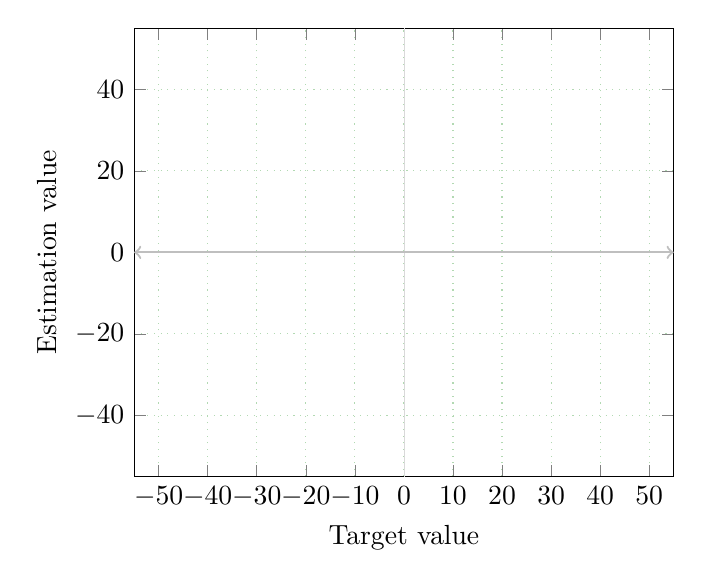
\begin{tikzpicture}%[rotate=90]
\expOneScatterPlot{Spherical-TwoDimensional-Estimation}{trialTargetValue}{trialReleasePositionTargetDiff}{}{
ylabel={Estimation value}, 
ymin=-55, ymax=55
}
\end{tikzpicture}	
\caption{E2: Spherical-TwoDimensional-Estimation}
\label{figure:expTwoTwoDimSphericalDuration}			
\end{figure}

\begin{figure}[!ht]
\centering
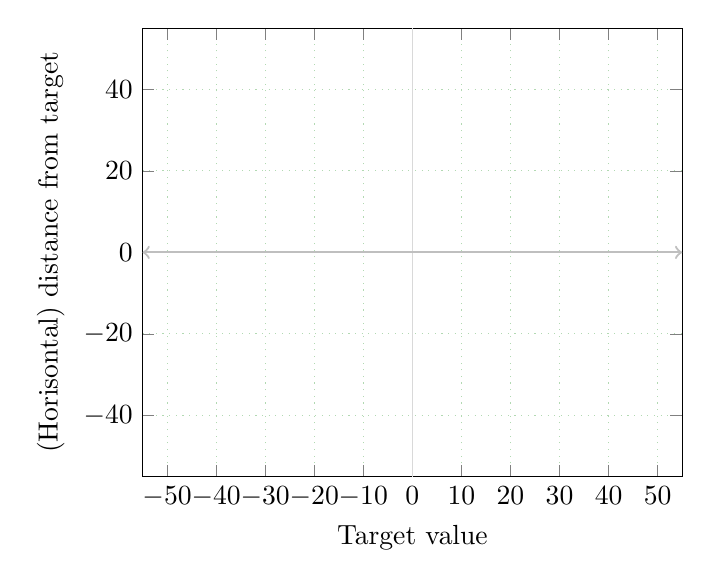
\begin{tikzpicture}
\expOneScatterPlot{Spherical-Horisontal-Estimation}{trialTargetValue}{trialReleasePositionTargetDiff}{}{
ylabel={(Horisontal) distance from target}, 
ymin=-55, ymax=55,
}
\end{tikzpicture}	
\caption{E2: Spherical-Horisontal-Estimation}
\label{figure:expTwoTwoDimSphericalDuration}			
\end{figure}

\begin{figure}[!ht]
\centering
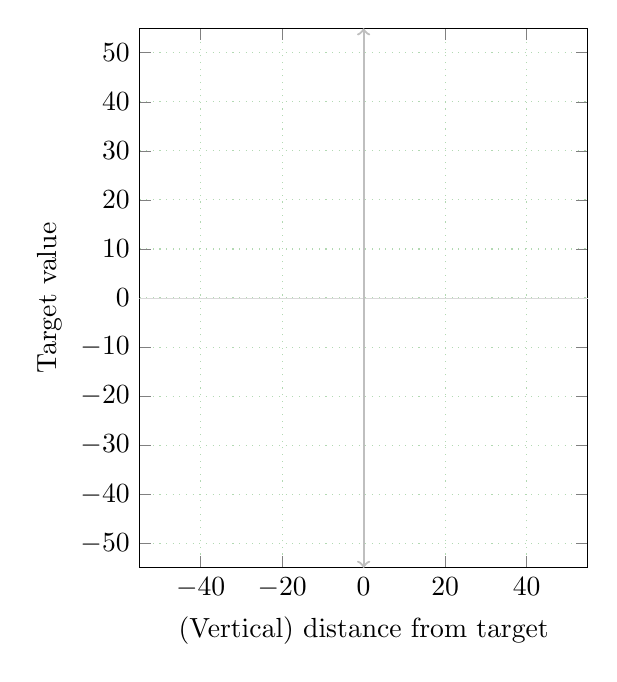
\begin{tikzpicture}[rotate=90, yscale=-1]
\expOneScatterPlot{Spherical-Vertical-Estimation}{trialTargetValue}{trialReleasePositionTargetDiff}{}{
ylabel={(Vertical) distance from target}, 
ymin=-55, ymax=55,
\perpAxesOptions
}
\end{tikzpicture}	
\caption{E: Spherical-Vertical-Estimation}
\label{figure:expTwoTwoDimSphericalDuration}			
\end{figure}


\end{comment}


%
\begin{tikzpicture}
     \draw[rotate=deg(0.5)] (0, 0) ellipse (0.5cm and 1.5cm);
\end{tikzpicture}





%
%
%\documentclass{article}
%\usepackage{pgfplots}
%\usepackage{datatool}
%\DTLloaddb[noheader=false]{coordinates}{data.csv}
%\pgfplotsset{compat=1.12}

%\usepackage{filecontents}

%
%\DTLloaddb[noheader=false]{coordinates}{testdata.csv}
%
%\begin{tikzpicture}	
%
%	\draw[
%	%	rotate=deg(\an),
%	color=orange,very thick] (0,0) ellipse [x radius=2,y radius=1,rotate around={deg(10):(0,0)}];
%
%
%%	\draw [help lines] (-2, -2) grid (2, 2);
%		\draw[step=1,help lines,black!20] (-0.95,-0.95) grid (4.95,4.95);
%		
%	
%	\begin{loopTabbedCsv}{coordinates}{\xc=xc, \yc=yc,\xr=xer,\yr=yer,\an=phi}
%
%	\draw[
%	%	rotate=deg(\an),
%		color=blue,very thick] (\xc, \yc) ellipse [x radius=\xr,y radius=\yr,rotate around={deg(\an):(\xc,\yc)}];
%
%
%	\end{loopTabbedCsv}
%
%%\end{axis}
%
%
%\end{tikzpicture}\\
%



\newcommand\plot[3]{
	\begin{tikzpicture}
	
	% help lines
	\draw[step=1,help lines,black!20] (-0.95,-0.95) grid (4.95,4.95);
	% axis
	\draw[thick,->] (-10,0) -- (10,0);
	\draw[thick,->] (0,-10) -- (0,10);
	
	% points
	\foreach \Point/\PointLabel in {#1}
	\draw[fill=green] \Point circle (0.05) node[above right] {$\PointLabel$};
	
	
	
%	\begin{scope}[xshift=1cm, yshift=2.075]
	
	\foreach \Point/\PointLabel in {#2}
	\draw[fill=red] \Point circle (0.05) node[above right] {$\PointLabel$};

%	\end{scope}
	

	
	#3	
	
	\end{tikzpicture}
	}


\plot{
		(1,2.3)/P0,(2.3,0.5)/P1,(3,2)/P2,(2.5,4.5)/P3
	}{
%		(0.07,1.2)/P0,(1.82,-0.17)/P1,(0.29,-0.81)/P2,(-2.19,-0.21)/P3
(-0.07,1.2)/P0,(-1.82,-0.17)/P1,(-0.29,-0.81)/P2,(2.19,-0.21)/P3
	}{
	\draw[->, thick, blue] 
%(2.2,2.325) -- (2.09100654418751,-0.39852149590928)
(2.2,2.325) -- (2.30899345581249,5.04852149590928)
	node[above right]{1};
	
	\draw[->, thick, orange] 
(2.2,2.325) -- (1.4771135144198,2.35392941962892)
	node[above right]{2};
	}


\plot{
(1,2.3)/P0,(-1,0.5)/P1,(3,2)/P2,(5,3.5)/P3
}{
(-0.82,0.62)/P0,(-3.38,-0.21)/P1,(0.88,-0.48)/P2,(3.32,0.07)/P3
}{
	\draw[->, thick, blue] 
	(2,2.075) -- (9.26955486324896,5.34430729026665)
	node[above right]{1};
	
	\draw[->, thick, orange] 
	(2,2.075) -- (1.91046489706353,2.27408815085112)
	node[above right]{2};
	
}



\begin{tikzpicture}

%	\def\Xmin{0}
%	\def\Ymin{-0.5}

	\begin{axis}[
%	xmin=\Xmin,
%	ymin=\Ymin,
	xmax=50,ymax=50,
	xmin=-50,ymin=-50,
%	domain=-50:50
	]

%	\addplot table [x=xc, y=yc, col sep=comma, only marks, mark=0] {testdata.csv};
%	

%	\draw[red] (-2,1.5) node[anchor=south] {.};


	\addplot table [x=xc, y=yc, col sep=comma, only marks, mark=0] {testdata.csv};
	
	
%	\draw[red] (1,2.3) node {.}
	
%	,{2.3,0.5},{3,2},{2.5,4.5}

%	\begin{loopTabbedCsv}{coordinates}{\xc=xc, \yc=yc,\xr=xer,\yr=yer,\an=phi}
%	
%	%	\draw[rotate=deg(\an)] (\xc, \yc) ellipse (0.5cm and 1.5cm);	
%	%	%		\draw[rotate=deg(\an)] (0, 0) ellipse (0.5cm and 1.5cm);	
%	%	%
%	%	
%	%	\filldraw[blue,fill opacity=0.2] (axis cs:\xc,\yc) ellipse;
%	
%%	(\xc,\yc)
%
%		\filldraw[blue,fill opacity=0.2] (axis cs:2,2) ellipse (0.5cm and 1.5cm);
%
%	
%	\end{loopTabbedCsv}



%	\pgfplotsextra{\DTLforeach*{coordinates}{\x=xc, \y=yc,\xr=xer,\yr=yer,\an=phi}{
%			%x-coor ellipse center, y-coor ellipse center, x-radius of ellipse, y-radius of ellipse, rotation angle of ellipse
%%			\filldraw[blue,fill opacity=0.2] 
%%			(axis cs:\x,\y) ellipse [x radius=\xr,y radius=\yr,rotate around={deg(\an):(\Xmin,\Ymin)}];
%		}
%	}
	
	
	\end{axis}
\end{tikzpicture}

\twocolumn



%%\pgfplotstableread{\expTwoPolarCsvFilepath}{\expTwoData}


\def\pcaFilepath{data/exp1/PCA.csv}



\loadTabbedCsv{Pca}\pcaFilepath
\loadTabbedCsv{PcaAggregated}{data/exp1/PCA-aggregated.csv}


%%% DEVICE PARAMS
\def\deviceFilepath{data/exp1/device.csv}	
\loadTabbedCsv{Device}\deviceFilepath	
%%%




\loadTabbedCsv{PcaTarget50}{data/exp1/PCA-targetValue(50).csv}


\def\PPM{10} % i,e. 851

\newcommand\drawOnscreenDims[1][fill=red!40, draw=red, opacity=0.2]{
	\coordinate (origin) at (axis cs:0,0);			    
	\pgfplotsextra{\DTLforeach*{Device}{\onscreenPixelHeight=onscreenPixelHeight, \onscreenPixelWidth=onscreenPixelWidth}{
			%	\edef\onscreenPixelHeight{\onscreenPixelHeight}
			%	\edef\onscreenPixelWidth{\onscreenPixelWidth}
			\filldraw[#1] ($(origin) - (.5*\onscreenPixelWidth/\PPM,.5*\onscreenPixelHeight/\PPM)$) rectangle ($(origin) +  (.5*\onscreenPixelWidth/\PPM,.5*\onscreenPixelHeight/\PPM)$);	
		}}
	}


% E2 July 10: [2016-07-10 20:10:20 INFORMATIONAL] TestPage: Offscreen rect: (0.223457493299726,-0.16266075098759,1.68620133133376) -- (0.228854267516688,-0.167606074963504,1.77226374528067) -- (0.179204979256355,-0.191535168366078,1.68731712014177) -- (0.184601753473317,-0.196480492341992,1.77337953408869)




%\readCsvFiltered{\expTwoCsvFilepath}{
%%	tablefilter in={sessionName}{evan},
%%	columns={sessionName, sessionType, trialUIAngle, trialIsStatistic, trialFinalOffscreenX, trialFinalOffscreenY,  trialFinalOffscreenZ},
%%	tablefilter in={sessionType}{E2},
%%	tablefilter in={trialUIAngle}{1.0471975511966},
%%	tablefilter in={sessionName}{Lily},
%%	tablefilter in={sessionName}{Lily},
%	tablefilter in={sessionName}{evan},
%	tablefilter out={trialIsStatistic}{1},
%%	tablefilter in={trialDurationSecondsIsOutlier}{0}
%	}\expTwoData
%%\pgfplotstableread{test.dat}{\expTwoData}




%\pgfplotstablesort[sort key={trialFinalOffscreenY}]{\sorted}{\total} %get the data and sort by column 'T'

%\pgfplotstablesort[sort key={trialFinalOffscreenY}]{\sorted}{\expTwoData} %get the data and sort by column 'T'


\def\strangeScale{1/10}


%\def\participantName{Lily}
%\def\participantName{rose}
%\def\participantName{evan}
\def\participantName{rose}
\def\participantColor{\leahColor!50}
\pgfplotstableread{data/exp1/TrialSesssions-(E2-\participantName).csv}{\releaseSpaceData}


\pgfplotstableread{data/exp1/TrialSesssions-(E2-evan).csv}{\dataTwoEvan}
\pgfplotstableread{data/exp1/TrialSesssions-(E2-rose).csv}{\dataTwoRose}
\pgfplotstableread{data/exp1/TrialSesssions-(E2-leah).csv}{\dataTwoLeah	}
\pgfplotstableread{data/exp1/TrialSesssions-(E2-Lily).csv}{\dataTwoLily}
\pgfplotstableread{data/exp1/TrialSesssions-(E2-soniaa).csv}{\dataTwoSonia}
\pgfplotstableread{data/exp1/TrialSesssions-(E2-mikee).csv}{\dataTwoMike}


\begin{figure*}[!ht]
	%	\def\domainMax{1.2}
	\centering
%%%%%%%%%%%%%%%%	
%%%%%%%%%%%%%%%%	
%%%%%%%%%%%%%%%%	
%%%%%%%%%%%%%%%%	
%%%%%%%%%%%%%%%%	
%%%%%%%%%%%%%%%%	
%%%%%%%%%%%%%%%%	
%%%%%%%%%%%%%%%%	
%%%%%%%%%%%%%%%%	
%%%%%%%%%%%%%%%%	
%%%%%%%%%%%%%%%%	
%%%%%%%%%%%%%%%%	
%%%%%%%%%%%%%%%%	
%%%%%%%%%%%%%%%%	
%%%%%%%%%%%%%%%%	
%%%%%%%%%%%%%%%%	
%%%%%%%%%%%%%%%%	
%%%%%%%%%%%%%%%%	
		\fullPageReleaseSpacePlots
%	\end{scaletikzpicturetowidth}
\caption{Final locations with respect to the axis formed by the device callibration (axis units in meters).}
\label{figure:expOneTwoBaselineTwoDimDurationAll}			
\end{figure*}



%\begin{figure*}[!ht]
%%	\def\domainMax{1.2}
%	\centering
%%	\def\participantName{Lily}
%	\twoFigure{
%		\hspace*{-2cm}
%		\begin{tikzpicture}[scale=1.15]%[rotate=90]
%			\releaseSpaceAxis[view={0}{90}]{
%				\releaseSpacePlotAllParticipants
%%				\releaseSpacePlot[\participantColor]{\releaseSpaceData}
%			}			
%		\end{tikzpicture}	
%	}{
%		\vspace*{-2cm}
%		\begin{tikzpicture}[scale=1.15]%[rotate=90]
%			\releaseSpaceAxis[view={20}{20}]{
%				\releaseSpacePlotAllParticipants
%%				\releaseSpacePlot[\participantColor]{\releaseSpaceData}
%			}
%		\end{tikzpicture}	
%	}
%	%	\end{scaletikzpicturetowidth}
%	\caption{Top-down view of final locations.}
%	\label{figure:expOneTwoBaselineTwoDimDurationAll}			
%\end{figure*}

% -----------------------------------



%\readCsvFiltered{\expOneCsvFilepath}{
%%	tablefilter in={sessionName}{evan},
%%	columns={sessionName, sessionType, trialUIAngle, trialIsStatistic, trialFinalOffscreenX, trialFinalOffscreenY,  trialFinalOffscreenZ},
%	tablefilter in={sessionType}{E2},
%%	tablefilter in={trialUIAngle}{1.0471975511966},
%%	tablefilter in={sessionName}{Lily},
%	tablefilter out={sessionName}{mean},
%%	tablefilter out={trialIsStatistic}{1},
%%	tablefilter in={trialDurationSecondsIsOutlier}{0}
%	}\expTwoMeanData


%\pgfplotstablegetrowsof{\expTwoMeanData}
%\pgfmathsetmacro{\N}{\pgfplotsretval-1}  
%\foreach \angle in {0,1,2,,...,360} {
%	\definecolor{degreeColor\angle}{hsb}{\angle/360, 1, 1}
%}

\newcommand\expPolarPlotAngles{
	\expPolarPlotAngle{0}
	\expPolarPlotAngle{30}
	\expPolarPlotAngle{60}
	\expPolarPlotAngle{90}
	\expPolarPlotAngle{120}
	\expPolarPlotAngle{150}
}

\begin{figure*}	
	\begin{centering}
		
	\hspace*{-1cm}			
	\twoFigure{		
%		\hspace*{-0.22cm}
		\begin{tikzpicture}[scale=1.2]
%		\hspace*{-0.22cm}
		\expPolarAxis[		
			extra y tick labels={ 0.5m, 0, -0.5m},					
			y dir=reverse,  %%% REVERSE BECAUSE TRACKER VIEWS FROM OPPOSITE SIDE!		
			]{	
				\drawCircles
				
				\expPolarPlotAngles
%					
%				\expPolarPlotAngle{0}
%				\expPolarPlotAngle{30}
%				\expPolarPlotAngle{60}
%				\expPolarPlotAngle{90}
%				\expPolarPlotAngle{120}
%				\expPolarPlotAngle{150}
				
				\begin{scope}[yscale=-1] % to get the axis labels positioned correctly
					\polarPlotDrawRadials				
				\end{scope}						
				
				\drawOnscreenDims
%			\plotPcaRings

		}	
		\end{tikzpicture}
	}{
	\hspace{1cm}
		\begin{tikzpicture}[scale=1.2]	
		\expPolarAxis[			
			extra y tick labels={ 0.5m, 0, -0.5m},					
			y dir=reverse,  %%% REVERSE BECAUSE TRACKER VIEWS FROM OPPOSITE SIDE!
%			extra y tick labels=,	
%				hide y axis,ymajorgrids=true,yminorgrids=true,
			]{		
			\drawCircles
				

				
			\expPolarPlotAngleAlt{0}
			\expPolarPlotAngleAlt{30}
			\expPolarPlotAngleAlt{60}
			\expPolarPlotAngleAlt{90}
			\expPolarPlotAngleAlt{120}
			\expPolarPlotAngleAlt{150}
			
			\begin{scope}[yscale=-1] 
				\polarPlotDrawRadials 
			\end{scope}			
				
			\drawOnscreenDims

%				\draw[
%				%	rotate=deg(\an),
%				color=blue,very thick] (axis cs:0,0) ellipse [x radius=40.58140,y radius=32.07781,
%%				rotate around={deg(148):(9.4,28.8)}
%				%				rotate around={deg(148):(50,0)}
%				];

%				\draw[dashed, ->, color=brown,very thick] (origin) -- +(100,100); 			
%				\draw[dashed, ->, color=pink,very thick] (origin) -- +(10,10); 
			
%				\draw[color=blue,very thick] ($(origin) + (5.0, 4.7)$) ellipse [x radius=57,y radius=65,
%				rotate around={deg(17):(5.0,4.7)}
%				%				rotate around={deg(148):(50,0)}
%				];



	
%			\draw[
%			%	rotate=deg(\an),
%			color=orange,very thick] (axis cs:0,28.8) ellipse [x radius=405.8140,y radius=320.7781,
%			rotate around={deg(148):(9.4,28.8)}
%			%				rotate around={deg(148):(50,0)}
%			];

		}		
		\end{tikzpicture}
	}
	\end{centering}
	\caption{TT: Mean estimations of target value locations, with each estimation mean indicated by color and arrow towards the true location. The two plots are identical except  for the color convention used, where the coloring of the left plot  illustrates the distribution of estimations for each (absolute) target value and the coloring og the right gives the distribution for each angle.}
	\label{figure:expOneBaselineDuration}				
\end{figure*}

\begin{figure*}	
	\centering
%		\hspace*{-1cm}			
%		\twoFigure{		
%			%		\hspace*{-0.22cm}
	\begin{tikzpicture}[scale=1.2]
		%		\hspace*{-0.22cm}
		\expPolarAxis[		
		extra y tick labels={ 0.5m, 0, -0.5m},					
		y dir=reverse,  %%% REVERSE BECAUSE TRACKER VIEWS FROM OPPOSITE SIDE!		
		]{	
			
			\begin{scope}[yscale=-1] 
				\polarPlotDrawRadials 
			\end{scope}			
							
							
			\plotReleasePositionsColorByTarget			
					
	%		\coordinate (origin) at (axis cs:0,0);			    
						
			\plotPcaRings
					
			\drawOnscreenDims
		}	
		\end{tikzpicture}
		\caption{The projected locations onto the sphere (i.e. not equivalent to a top-down view - release height changes location). Color codings are target values.}
%		\label{figure:}				
\end{figure*}








\begin{figure*}	
	\centering
	%		\hspace*{-1cm}			
	%		\twoFigure{		
	%			%		\hspace*{-0.22cm}
	\begin{tikzpicture}[scale=1.2]
	%		\hspace*{-0.22cm}
	\expPolarAxis[		
	extra y tick labels={ 0.5m, 0, -0.5m},					
	y dir=reverse,  %%% REVERSE BECAUSE TRACKER VIEWS FROM OPPOSITE SIDE!		
	]{	
		
		\begin{scope}[yscale=-1] 
		\polarPlotDrawRadials 
		\end{scope}			
		
		\drawOnscreenDims
		
%		\plotReleasePositionsColorByTarget			
		
		
		
		%		\coordinate (origin) at (axis cs:0,0);			    
		
%	\plotPcaRings
	
	
	\coordinate (origin) at (axis cs:0,0);			    
%	\def\PPM{10} % i,e. 851
%%	\foreachTabbedCsvRowInPlot
	\pgfplotsextra{\DTLforeach*[\DTLiseq{\target}{50}]{Pca}{\xc=x, \yc=y,\xr=xr,\yr=yr,\circleAngle=deg,\target=target,\circleRadius=circleRadius,\circleRadiusM=circleRadiusM}{	
			
			
			\coordinate (circlePos) at ($(origin) + (\xc/\PPM, \yc/\PPM)$);
			%			\node[mark size=0.02cm,color=\targetColor\target] at (circlePos) {\pgfuseplotmark{triangle*}};
			\draw (circlePos) node[cross, rotate around={-1*\circleAngle-45:(circlePos)},color=\targetColor\target] {};		

			% ellipse	
			\draw[color=\targetColor\target,very thick] ($(origin) + (\xc/\PPM, \yc/\PPM)$) ellipse [
				x radius=\xr/\PPM,
				y radius=\yr/\PPM,
				rotate around={-1*\circleAngle:(circlePos)} %				rotate around={deg(148):(50,0)}
				];
				
			% circle radius text and line
			\draw[black!80,<->,thick] (origin) -- +($(\circleRadius/\PPM,0)$);
			\node[align=left, fill=white,text=black!80] at ($(origin)  + (0.5*\circleRadius/\PPM,0)$) {\scriptsize $\circleRadiusM$m};
%					
			% circle at mean
			\draw[color=\targetColor\target,thick,dashed,opacity=0.2] (circlePos) ellipse [
			x radius=\circleRadius/\PPM,
			y radius=\circleRadius/\PPM
			];
			% circle at origin
			\draw[color=\targetColor\target] (origin) ellipse [
				x radius=\circleRadius/\PPM,
				y radius=\circleRadius/\PPM
				];
	}}
	
			
	}	
	\end{tikzpicture}
	\caption{Determining the radius, cutoff target=40 TODO!}
	%		\label{figure:}				
\end{figure*}



\begin{figure*}	
	\centering
	%		\hspace*{-1cm}			
	%		\twoFigure{		
	%			%		\hspace*{-0.22cm}
	\begin{tikzpicture}[scale=1.2,>=stealth]
	%		\hspace*{-0.22cm}
		\expPolarAxis[		
		extra y tick labels={ 0.5m, 0, -0.5m},					
		y dir=reverse,  %%% REVERSE BECAUSE TRACKER VIEWS FROM OPPOSITE SIDE!		
		]{	
			
		\begin{scope}[yscale=-1] 
			\polarPlotDrawRadials[lightgray, dashed, shorten >=.03cm, shorten <=.4cm, opacity=0.3] 
		\end{scope}			
			

		%% ELLIPSES 			
		\addplot[
%			red,
			scatter,
			only marks,
			opacity=0.75,
			mark size=0.3,
			point meta=explicit symbolic,
			scatter/classes={
				10=\targetColor{10},
				20=\targetColor{20},
				30=\targetColor{30},
				40=\targetColor{40},
				50=\targetColor{50} %				50={mark=*,\targetColor{50},line width=1mm, draw=\targetColor{50}}							
			}					
			] 	
			table[
			x=x,
			y=y,	
			meta=target
			,filter in={type}{ellipse}					
%			filter in={target}{50}					
			] {data/exp1/skewedCircles.csv};	


		%% ELLIPSES 			
		\addplot[
		%			red,
		scatter,
		only marks,
		opacity=0.75,
		mark size=0.8,
		point meta=explicit symbolic,
		scatter/classes={
			10=\targetColor{10},
			20=\targetColor{20},
			30=\targetColor{30},
			40=\targetColor{40},
			50=\targetColor{50} %				50={mark=*,\targetColor{50},line width=1mm, draw=\targetColor{50}}							
		}					
		] 	
		table[
		x=x,
		y=y,	
		meta=target
		,filter in={type}{radial},				
					filter in={target}{50}					
		] {data/exp1/skewedCircles.csv};	
		
		

%			\loadTabbedCsv{..}\path	
%			\pgfplotsextra{\DTLforeach*[\DTLiseq{type}{radial}\DTLiseq{targt}{50}]{}{\xc=x}{
%					
%			}}


		
		
		%			\loadTabbedCsv{..}\path	
		%			\pgfplotsextra{\DTLforeach*[\DTLiseq{type}{radial}\DTLiseq{targt}{50}]{}{\xc=x}{
		%					
		%			}}

		%% RADIALS			
		\addplot[
		%			red,
		scatter,
		only marks,
		mark size=0.1,
%		red,
		point meta=explicit symbolic,
		scatter/classes={
%			ellipse=transparent, %{mark=*,gray,line width=1mm}							
			radial={black!50, dashed} %{mark=*,gray,line width=1mm}							
		}					
		] 	
		table[
		x=x,
		y=y,	
		meta=type,
		filter in={type}{radial},					
%		filter in={target}{50}					
		] {data/exp1/skewedCircles.csv};	
		
						\begin{scope}[yscale=-1] 
						\polarPlotDrawRadials 
						\end{scope}			
									\drawCircles
									
									
			
		
		
%								\angle30x=angle30x,
%								\angle30y=angle30y,
%								\angle60x=angle60x,
%								\angle60y=angle60y,
%								\angle90x=angle90x,
%								\angle90y=angle90y,
%								\angle120x=angle120x,
%								\angle120y=angle120y,
%								\angle150x=angle150x,
%								\angle150y=angle150y
%								
			\coordinate (origin) at (axis cs:0,0);			    
%			\def\PPM{10} % i,e. 851
			%%	\foreachTabbedCsvRowInPlot
			\pgfplotsextra{\DTLforeach*[\DTLiseq{\target}{50}]{Pca}{\xc=x, \yc=y,\xr=xr,\yr=yr,\circleAngle=deg,\target=target,\circleRadius=circleRadius,\circleRadiusM=circleRadiusM,
					\angleAx=angle0x,
					\angleAy=angle0y,
					\angleBx=angle30x,
					\angleBy=angle30y,
					\angleCx=angle60x,
					\angleCy=angle60y,
					\angleDx=angle90x,
					\angleDy=angle90y,
					\angleEx=angle120x,
					\angleEy=angle120y,
					\angleFx=angle150x,
					\angleFy=angle150y,
					\angleGx=angle180x,
					\angleGy=angle180y,
					\angleHx=angle210x,
					\angleHy=angle210y,
					\angleIx=angle240x,
					\angleIy=angle240y,
					\angleJx=angle270x,
					\angleJy=angle270y,
					\angleKx=angle300x,
					\angleKy=angle300y,
					\angleLx=angle330x,
					\angleLy=angle330y}{	
								
%				\coordinate (circlePos) at ($(origin) + (\xc/\PPM, \yc/\PPM)$);
				\coordinate (circlePos) at ($(origin) + (\xc/\PPM, \yc/\PPM)$);
				%			\node[mark size=0.02cm,color=\targetColor\target] at (circlePos) {\pgfuseplotmark{triangle*}};
				\draw (circlePos) node[cross,
					rotate around={-1*\circleAngle-45:(circlePos)},
					color=\targetColor\target] {};		
				
				
				
				%% ELLIPSES
				
				
				
				\draw[\targetColor{50}, fill=lightgray, opacity=0.082] ($(origin) + (\xc/\PPM, \yc/\PPM)$) ellipse [
				x radius=\xr/\PPM,
				y radius=\yr/\PPM,
				rotate around={-1*\circleAngle:(circlePos)} 
				];

%				\newcommand\drawEllipse{
%					\draw[color=\targetColor{\currentAngle0}] ($(origin) + (\xc/\PPM, \yc/\PPM)$) ellipse [
%					x radius=\currentAngle*\xr/\circleRadius*\targetTickDistance/\PPM,
%					y radius=\currentAngle*\yr/\circleRadius*\targetTickDistance/\PPM,
%					rotate around={-1*\circleAngle:(circlePos)} %				rotate around={deg(148):(50,0)}
%					];
%				}
%				\edef\currentAngle{1}\drawEllipse
%				\edef\currentAngle{2}\drawEllipse
%				\edef\currentAngle{3}\drawEllipse
%				\edef\currentAngle{4}\drawEllipse
%				\edef\currentAngle{5}\drawEllipse


				
				%% RADIALS
%%				, path fading=west, fading angle=30
%				\newcommand\drawSkewedRadials{				
%					\draw[lightgray, dashed, shorten >=.03cm, shorten <=.12cm] (circlePos) -- ($(origin) + (\angleAx/\PPM,\angleAy/\PPM)$) node[right]{\scriptsize 0};% node[circle,fill,inner sep=1pt]{}; 
%					\draw[lightgray, dashed, shorten >=.03cm, shorten <=.12cm] (circlePos) -- ($(origin) + (\angleBx/\PPM,\angleBy/\PPM)$) node[above right]{\scriptsize 30}; 
%					\draw[lightgray, dashed, shorten >=.03cm, shorten <=.12cm, path fading=west, fading angle=60] (circlePos) -- ($(origin) + (\angleCx/\PPM,\angleCy/\PPM)$) node[above right]{\scriptsize 60}; 
%					\draw[lightgray, dashed, shorten >=.03cm, shorten <=.12cm, path fading=west, fading angle=90] (circlePos) -- ($(origin) + (\angleDx/\PPM,\angleDy/\PPM)$) node[above]{\scriptsize 90}; 
%					\draw[lightgray, dashed, shorten >=.03cm, shorten <=.12cm, path fading=west, fading angle=120] (circlePos) -- ($(origin) + (\angleEx/\PPM,\angleEy/\PPM)$) node[above left]{\scriptsize 120}; 
%					\draw[lightgray, dashed, shorten >=.03cm, shorten <=.12cm, path fading=west, fading angle=150] (circlePos) -- ($(origin) + (\angleFx/\PPM,\angleFy/\PPM)$) node[above left]{\scriptsize 150}; 
%					\draw[lightgray, dashed, shorten >=.03cm, shorten <=.12cm, path fading=west, fading angle=180] (circlePos) -- ($(origin) + (\angleGx/\PPM,\angleGy/\PPM)$) node[left]{\scriptsize 180}; 
%					\draw[lightgray, dashed, shorten >=.03cm, shorten <=.12cm, path fading=west, fading angle=210] (circlePos) -- ($(origin) + (\angleHx/\PPM,\angleHy/\PPM)$) node[left]{\scriptsize 210}; 
%					\draw[lightgray, dashed, shorten >=.03cm, shorten <=.12cm, path fading=west, fading angle=240] (circlePos) -- ($(origin) + (\angleIx/\PPM,\angleIy/\PPM)$) node[left]{\scriptsize 240};  
%					\draw[lightgray, dashed, shorten >=.03cm, shorten <=.12cm, path fading=west, fading angle=270] (circlePos) -- ($(origin) + (\angleJx/\PPM,\angleJy/\PPM)$) node[above right]{\scriptsize 270}; 
%					\draw[lightgray, dashed, shorten >=.03cm, shorten <=.12cm, path fading=west, fading angle=300] (circlePos) -- ($(origin) + (\angleKx/\PPM,\angleKy/\PPM)$) node[below right]{\scriptsize 300}; 
%					\draw[lightgray, dashed, shorten >=.03cm, shorten <=.12cm, path fading=west, fading angle=330] (circlePos) -- ($(origin) + (\angleLx/\PPM,\angleLy/\PPM)$) node[below right]{\scriptsize 330}; 
%				}
%				\drawSkewedRadials
			}}
			%\shade[inner color=transparent,outer color=red!40] (0,0) rectangle (4,4);
			
	
			\drawOnscreenDims
%			\expPolarPlotAngles
%			\plotReleasePositionsColorByTarget			
		}	
	\end{tikzpicture}
	\caption{Determining the radius, cutoff target=40 TODO!}
	%		\label{figure:}				
\end{figure*}


%((((((((((
%\begin{loopTabbedCsv}{skod}{\xc=x, \yc=y,\xr=xr,\yr=yr,\circleAngle=phi,\target=target, \circleColor=color}
%	\target\\
%\end{loopTabbedCsv}
%))))))))



%	\begin{tikzpicture}
%	
%	% help lines
%	\draw[step=1,help lines,black!20] (-0.95,-0.95) grid (4.95,4.95);
%	% axis
%	\draw[thick,->] (-10,0) -- (10,0);
%	\draw[thick,->] (0,-10) -- (0,10);
%	
%	\end{tikzpicture}
%





\newcommand\expPolarPlotReleaseDiff[2]{%%%%%%%%TEST
%	\pgfmathdivide{#1}{180}
%	\definecolor{degreeColor#1}{hsb}{\pgfmathresult, 1, 1}
	\addplot[
		%		red,
		%			only marks,
		%	->,
		rotate around={#1:(axis cs:0,0)},
		%	shorten >=.15cm,
		%	shorten <=.15cm,
		ycomb,
		%	x dir=reverse, 
		%	scatter,
		ybar, bar width=4,
		fill=#2,%degreeColor#1!90,%red!30,
		point meta=explicit symbolic,
		%			red,
	%	scatter/classes={
	%		mean={mark=*,\myRed,line width=0mm},
	%		target={mark=*,\myGreen,line width=0mm}		
	%	}						
		]%surf, mesh/rows=10] 	
		plot[error bars/.cd, 
		y dir = both, y explicit,  	
		%	x dir = both, x explicit,  	
		%		error bar style={
		%			line width=1.5pt, 
		%			rotate around={30:(axis cs:\x,\y)},
		%			xshift=4.5mm
		%			},
		error mark options = {
			%		rotate around={#1:current origin} 
			%%		line width=1.5pt, 
			mark size = 0pt 
		},
		] %,bar width=3pt,
		table[
		x=trialTargetHorizontalDistanceFromOrigo,
		y=trialFromTargetToReleaseVerticalLength,
		y error=trialFromTargetToReleaseVerticalLengthConfidence,
		%	x error=trialFromTargetToReleaseVerticalLengthConfidence,
		meta=sessionName,
		filter in={sessionName}{mean},
		%			filter in={sessionType}{E2},
		filter in={trialUIAngleDegrees}{#1},
		%	filter in={trialTargetValue}{#2}
		%		filter in={trialUIAngle}{1.5707963267949}
		] 
		%			{data/exp1/TrialSesssions-(E2-polar-evan,rose,Lily,Lily).csv} 
		{\expTwoPolarCsvFilepath};	
}



\begin{figure}
	\centering
	\begin{tikzpicture}[scale=1.2]		
		\hspace*{-1cm}
		\expPolarAxis{		
			\polarPlotDrawRadials
			\drawCircles		
	
			\expPolarPlotReleaseDiff{0}{angle0}
			\expPolarPlotReleaseDiff{30}{angle30}
			\expPolarPlotReleaseDiff{60}{angle60}
			\expPolarPlotReleaseDiff{90}{angle90}
			\expPolarPlotReleaseDiff{120}{angle120}
			\expPolarPlotReleaseDiff{150}{angle150}
		}	
	\end{tikzpicture}
	\caption{A compact illustration that captures all combinations of mean target estimate deviations (Euclidean distance), along with 95\% confidence values (i.e. one bar for each pair and bars of same color resulting from input on the same angle.}
	\label{fig:experimentalSetupAbove}
\end{figure}

%\begin{figure*}
%	\twoFigure{		
%	}{
%	}
%\end{figure*}
%	
	
	

%\begin{figure*}	
%	\centering
%	\begin{tikzpicture}
%		\begin{axis}[ 
%			xmin=-55, 
%			xmax=55, 
%	%		ymin=0,
%	%		ymax=#4,
%	%		legend pos=outer north east,
%			xlabel={Target value},			
%			ylabel={Euclidean distance to target},			
%			y label style={
%%				rotate=-90,
%				%						yshift=50.
%	%			xshift=10
%			},
%			%		xscale=1.3,
%			%		yscale=1.3,
%	%		scale=0.9,
%			]
%		
%			\addplot[
%			%		red,
%			%			only marks,
%			%	->,
%			%	shorten >=.15cm,
%			%	shorten <=.15cm,
%%			ycomb,
%			%	x dir=reverse, 
%			%	scatter,
%%			ybar, bar width=4,
%			red,
%		%	fill=#2,%degreeColor#1!90,%red!30,
%			point meta=explicit symbolic,
%			%			red,
%			%	scatter/classes={
%			%		mean={mark=*,\myRed,line width=0mm},
%			%		target={mark=*,\myGreen,line width=0mm}		
%			%	}						
%			]%surf, mesh/rows=10] 	
%			plot[error bars/.cd, 
%			y dir = both, y explicit,  	
%			%	x dir = both, x explicit,  	
%			%		error bar style={
%			%			line width=1.5pt, 
%			%			rotate around={30:(axis cs:\x,\y)},
%			%			xshift=4.5mm
%			%			},
%			error mark options = {
%				%		rotate around={#1:current origin} 
%				%%		line width=1.5pt, 
%				mark size = 0pt 
%			},
%			] %,bar width=3pt,
%			table[
%			x=trialTargetValue,
%			y=trialReleasePositionTargetDiff,
%			y error=trialReleasePositionTargetDiffConfidence,
%			%	x error=trialFromTargetToReleaseVerticalLengthConfidence,
%		%	meta=sessionName,
%			filter in={sessionName}{mean}
%			] 
%			{data/exp1/TrialSesssions-(E2-mean,target).csv};	
%
%
%		\end{axis}
%	\end{tikzpicture}
%	\caption{Mean target diffs}
%		%		\label{figure:}				
%\end{figure*}




		
%\section{Abbreviations}
%\lipsum[2]


\twocolumn[
	\section{Introduction}\label{ch:introduction}
	]
	
	
\noi The use of tools is a  trademark of human history, both in simple times of mere survival and even more so in the establishment of societies and specializations of trades. This potential for people to gain from optimization through specialization is not the result of any obvious physical superiority. Quite the contrary, its stems from the ability to communicate abstract concepts over time, with the tool itself being nothing more than a momentary manifestation.

While the concept of a tool is abstract, its physical realization always takes some mechanized form intended for human interaction, one that usually  that draws on our most distinguished evolutionary advantage: the extraordinary  flexibility  and sensitivity of our hands and fingers. The computer is well-suited in this regard, due the lack of mechanics. The most remarkable human tool to date, it is capable of emulating the same logic that is embedded in all natural laws, but logic is all information and has no matter or motion. The application of logic, through algorithms that process  information, results in nothing but information itself. Not surprisingly, the physical activity needed to interact with a computer is also limited to information, provided through alphabetized languages for defining computational steps.

%And persisting that is close to instantaneous  through negligible physical differentia. 
% combinations of standardized letters of some alphabet.  

The most successful input methods reflect these observations, in the sense that they rely on the hands  to provide a vast array of combinatorial input with as little mechanical action as possible. In addition, the flexibility of modern displays help to rapidly  comprehend informational complexity, due to the fast perceptual speed of vision. Display technology has recently changed the way we interact with computers, due to quantum leaps in terms of quality, dimensionality and price reduction. As an obvious real-world example, mobile telephones  went from  panels of knobs and buttons to all display-based  miniature computers almost overnight  - \ti{mobile devices} that  incorporate a multitude of functions, each previously only available in some dedicated and more mechanical form factor. In other words, rapid progress in one technology facilitated the convergence of a multitude of others, such that a modern lifestyle now includes having a mobile device - using a pocket-size rectangular display to perform a wide variety of daily activities is now the norm. Not surprisingly, developments in user interface design principles have followed suit, with designers unanimously adopting a \ti{Mobile First}\cite{MobileFirst} paradigm that anticipates the most probable human-computer interaction as one based on mobile devices.

Although these minimalistic devices provide mobility, there are caveats. Designing an appropriate navigational user interface on touch-based devices cannot be approached with a one-size-fits-all paradigm, but must take into account some basic factors that greatly influences the user experience. As an imaginary example, a user dragging a map by touch on a large display will typically be positioned close to the center of the screen. Hence, with half or more of the displayed map in peripheral view, the user then has a good overview of the information space. This will obviously not apply in the case of a small portable device, where conditions are opposite - the display being in full view, but the presentation of input space severely restricted by the reduced dimensions of the display. Differing form factors therefore make for very different user experiences, with the smaller ones presumably resulting in a greater number of repetitive swipes and "tricks" to offset this, such as inertia. This represents a general problem that currently has no good solution: on a small touch screen, navigating to specific information usually requires many touch operations, due to the restricted input and presentation space. Clearly, this is an undesirable property of any user interface. Furthermore, the problem of increased input is exacerbated by the very fact that any touch operation is somewhat imprecise and tends to obscure the user interface for each interaction, since the input and display plane are the same. 

Hence, the information space that needs to be accessible for presentation within typical mobile applications usually exceeds the amount of display space available. User interface design usually deals with this issue through some form of strict prioritization,  presenting only what is considered most relevant to the current information need, along with the ability to navigate into other parts of the information space. Such designs therefore need input methods that allow for bringing specific parts of non-visible information into view, in a flexible and discrete manner that ideally minimizes obstruction of the display.

Looking forward, it would be reasonable to assume that any use of a tool that may alleviate these problems is highly relevant from a  research perspective. One clear contender here, is the use of  computer vision and pattern recognition, fields that have recently made tremendous progress.  These center around how natural human language, i.e. speech, body gestures and touch can be interpreted successfully to the extent that it may either serve as the sole input for controlling a computer or work in parallel with other types of input. With increasing gains in hardware, software and falling costs, the future applicability of computer vision is currently being anticipated through active research attempts at blending frontier technology with innovative thought. Naturally, the question arises as to whether or not this may be have any potential in mobile device interaction. For instance, what if the user's finger could be monitored, using computer vision, as it moves outside the boundaries of the display?\\

\subsection{Contributions}

%to test a hypothetical solution to the problem of navigating efficiently on small touch screens. 
The goal of the research undertaken here is to investigate a potential use of off-screen space for addressing the issues associated with small displays, as typically found on  smaller portable devices.  More specifically, the work explores  how a touch-screen operation (a \ti{swipe}) can extend beyond the display boundaries and into off-screen space. This leads to the question of how this space is to be defined, how the swipe transition from the display into this space will take place and how the efficiency and effect on the user experience is to be measured. 

Three experiments follows a learning path that first identifies an assumed optimal spatial interface, then explores this in more detail and finally attempts to optimize it based on observed properties of the true space. The first of these shows that incorporating off-screen space as if it was a sphere leads to a slight interaction time penalty, but also eliminates the need for redundancy and inertia. Second, if users are asked to perform estimations of spatial locations, it appears that the true space does in fact align with a sphere, but also has some inherent properties that differ. Third, modifying the interface to accommodate these properties shows a slight improvement in interaction time and serves as a potential starting point for further studies. 

  
\subsection{Organization}

This document has been organized as follows. Chapter \ref{ch:background} provides the background on current mobile devices, tracking technologies and existing work  related to the topic. In chapter \ref{ch:motivation}, the exact boundaries of what constitutes the goal, and what does not, is more formally defined, including the motivations and feasibility of the proposed solution. Next, assumptions and requirements of a solution that meets these goals are presented in chapter \ref{ch:approach}, including the reasoning and evolution of technology choices. Chapter \ref{ch:solution} enumerates the sequence of theoretical steps for solving the challenges involved with deriving a full solution. A brief commentary on the actual implementation is then given in chapter \ref{ch:implementation}. The data resulting from undertaking experiments with the implementation is then evaluated and interpreted in chapter \ref{ch:evaluation}. Lastly, thoughts and conclusions are given in the final chapter \ref{ch:conclusion}.


%which with increasing efficiency allows for the partial or total elimination of any mechanical or physical device for interacting with a computer. In other words, the search is on for the future of HCI and 







		  

\begin{comment} ### THESIS ##################################################

Not surprisingly however, a major drawback of mechanical devices is that they take the shape of moderately sized physical appendixes (often in the form of cheaply-made Asian plastics) and all but a few tend to require cumbersome wiring, with neither of these characteristics providing much in terms of portability or aesthetics. This has never posed a major problem in the traditional stationary desktop setup, but unfortunately don't go well with current trends that seek to embed minimalistic digital technology in every aspect of life. The future of computational devices is therefore expected to depend heavily on infusing minimalism into the design of \ti{cross-over devices} such as \ti{ultrabooks}\fn{A term introduced by Intel for categorizing an evolving class of laptops that are very thin, battery-efficient, and use low-voltage processors. Previously known as \ti{CULV laptops} (consumer ultra-low-voltage processors).} or entirely new devices, such as the widely adopted \ti{smart phone}, with both of these developments made possible by the realization of Moore's law\fn{A widely cited article\cite{Moore} that has recurrently served as predictor of computational performance trends for the past 50 years.} and four decades of innovation in silicon semiconductor manufacturing technology. 

In addition to their practical deficiencies, this inherent "clunkiness" of traditional interaction devices also fail from a health perspective. This is typically seen as the widespread tendency of computer users to contract neurological conditions, such as \ti{carpal tunnel syndrome}, which essentially result from the use of redundant physical patterns that the devices themselves strictly rely on. This over-exploitation of repetitive movement patterns is in fact a significant departure from the varied ways that human beings would normally interact with their natural surroundings, which further underlines the problematic nature of traditional human-computer interaction.


As a result, conditions have long been ripe for one or more evolutionary leaps within the field of human-computer interaction and the lack of accessible alternatives to overcome the obstacles associated with tradition currently represents a problem, even for those users with a moderate need for interacting with computer technology. 

############################################################# 
\end{comment}  

%\subsection{Future input methods}

\begin{comment} ### THESIS ##################################################

Intuition has always been center in the quest for future devices in human-computer interaction. An obvious example of this is the invention of the computer mouse, which represented a major breakthrough in usability and deserves partial credit for the popularization and rise of the personal computer in the 1980s. Th concept of the mouse remains largely unchanged to this day and has accumulated extensive (and still relevant) research on its usage patterns in standard desktops. In the early 1990s, about a decade after commercial mice became available and with the use of personal computer rocketing off, it was showed by  Johnson et al.\cite{MouseUsage} that people rely quite heavily on complementing keyboard input with the more intuitive and visual mouse. For a natural mix of varied computer tasks and people, it was shown that mouse usage composes between one third and up to two thirds of all input and represents an integral part of the user experience, rather than the occasional exception.  

This result illuminated that intuition cannot be downplayed in favor of efficiency, by assuming that human behavior will naturally gravitate towards what is theoretically optimal. For instance, relying solely on the keyboard for all input represents a highly efficient solution in terms of speed and physical effort, although this fact obviously has little effect on neither the majority of computer users, nor the design of the operating systems they commonly use\fn{Even within the world of keyboard devices, the statistically highly efficient Dvorak layout has failed to become the standard due to tradition, which again is a human factor.}. Hence, intuition should be viewed as a key criteria in the bi-directional play of forces between design that appeals to human behavior and inputs that allow for efficiently operating a modern computer, which at its core, is nothing but logical transitions between a set of states.

Yet, the field of interaction has been at a standstill for many years, with keyboard and mice dominating the desktop\fn{Alternatives (such as trackballs, touch-pads, electronic pens etc.) exist, although haven't gained widespread use and are all limited to interactions in two dimensions only. }.  Recent technological advancements have however managed to bridge the gap between the shortcomings of the past and an array of new ideas for what the future may hold within the field of interaction. One of the major foundations of this new progress is \ti{computer vision}, which may appropriately be described as the result of a cataclysm between existing research and broad gains in computational power, especially on consumer-level. More precisely, the ability of an algorithm to recognize and categorize visual cues, such as physical shapes or human gestures, relies heavily on searching a hypothesis space that scales far beyond what is computationally feasible, given narrow time constraints. For instance, the task of locating a hand within an image with reasonable certainty will typically rely on a mix of algorithms, of which one candidate may very well be \ti{support vector machines}\cite{Bishop} (SVMs). For the example of SVMs, these have been around for more than 50 years, but have gained immense popularity in recent years, due to their ability of efficiently performing classification and regression in very high dimensional spaces\fn{I.e. when employed with \ti{kernel methods}\cite{Bishop}.}. Hence, computer vision and pattern recognition is in fact a well-established research tradition, but with newfound applicability due to the rise of big data\fn{A broad term coined in 1997\cite{BigData}, here to be understood as extremely large data sets that may be analysed computationally to reveal patterns, trends, and associations, especially relating to human behaviour and interactions.} and increased availability of computational power.

############################################################# 
\end{comment}  


\begin{comment} ### THESIS ##################################################

\subsection{Applicability of computer vision}

The utility of computer vision's ability in recognizing visual cues reaches far beyond simply disrupting existing input methods. It has broad impact on all industries that rely on interacting with computers and even opens up new commercial opportunities for incorporating digital technology into areas where its use has previously been hindered by the lack of appropriate input methods.

For instance, the medical establishment has long since adopted the use of computers for the goal of achieving medical results that are beyond human capability. One typical example of this is the application of pattern recognition to imaging scans of patients, in order to estimate likelihoods of various types of disease (a textbook example within the field of statistical learning). Another is the optimization of surgical accuracy by guiding robotics, which minimizes incisions and tissue damage, thus allowing the patient for a faster recovery and resumption of daily activities. These two examples are particularly interesting, because advancements within the first has blended into the latter; imaging modalities are now the foundation of complex computer applications that directly guide surgical procedures, by overlaying radiologic imaging data onto the operative visualization system using computer vision. This concept, known as \ti{augmented reality}, can guide the surgeon's dissection path, by demonstrating vital anatomic structures beyond the visible surface, thereby providing a sense of depth that increases the probability of a successful outcome\cite{RobotsInSurgery}.

Another area of great potential is the inclusion of demographic groups that for one reason or another are not able to operate mechanical devices. This may include those that are suffering from certain types of disabilities or simply elderly people that are unable to learn how to interact with standard input devices, such as keyboard or mice. As such, any innovation that allows for more intuitive human-computer interaction, e.g. touch, speech or visual cues, would in fact open up the opportunity for certain individuals to enter the digital era, where they could not before.

############################################################# 
\end{comment}  

%\subsection{The problem with touch}

\begin{comment} ### THESIS ##################################################

The elimination of mechanical input has gained huge momentum within the domain of graphical user interfaces in recent years, largely due to the proliferation of relatively robust and innovative devices on consumer-level. As a result, a wide variety of touch-based devices now exist and a common denominator to them all is the portability and compactness that they pack by way of eliminating (or virtualizing) the traditional keyboard and mouse. Furthermore, this new generation of touch-based devices all offer one obvious feature that has become their signature and unique selling point; associating specific types of \ti{multi-touch} input with corresponding navigational actions, made possible by the application of pattern recognition\cite{Wood}. 

While the innovative features of touch input and gesture navigation are common to most of today's mobiles devices, what is not however, is their display sizes. Thus, the presentation space of these devices vary widely from that of large displays with dimensions measured in meters (e.g. interactive \ti{SMART boards}) to small smart phones with displays that measure no more than a few inches. Furthermore, they also differ in terms of processing capability, which greatly affects responsiveness, and finally, may have differing spacial orientations (e.g. the horizontally placed Microsoft Pixelsense table\fn{Previously known under the product name \ti{Surface}.}).

For these reasons, 

############################################################# 
\end{comment}  

\begin{comment} ### THESIS ##################################################

\subsection{Sensors on the rise}

Given the computer industry's rapidly increasing tendency to incorporate various types of sensors into newer designs, it would not be unreasonable to assume that pattern recognition will be deeply embedded within future operating systems. This is in fact already the case, as fingerprints and facial recognition are now being actively used to unlock smart phones\fn{As has been implemented by Apple and Samsung, respectively.}. Hence, it's not unfathomable that the spatial awareness of mobile devices will soon encompass the ability to sense the user's off-screen hand gestures. One could even speculate that one form of this may be facilitated by the upgrading of current front-facing cameras to \ti{fish-eyes}, i.e. cameras with a view angle of 360\textdegree. If so, computer vision could be used to provide a natural extension of the information space beyond the dimensions of the display, a concept that may prove to be particularly powerful for small devices such as smart phones and tablets, where space is scarce.

############################################################# 
\end{comment}  



\section{Background}
		  
\subsection{Information needs}

Today, the dominating mechanism for reflecting an application state is that of visual feedback, commonly done using the all affordable flat and square display technologies. Unfortunately, the \ti{infomation space} that ideally needs to be accessible for presentation within typical applications often exceeds the amount of display space available. This is typically dealt with by presenting the user with only the information considered relevant to the user's current need, along with the ability to navigate into other parts of the space using any number of differing input methods. However, for these navigational mechanisms to be successful, they need not only be versatile in their ability to navigate, but also discrete enough to not interfere with the information space to be reflected.

\subsection{Current input methods}

Navigational mechanisms have traditionally been implemented by making the user interact with dedicated mechanical devices that draw on our most distinguished evolutionary advantage: the ability to produce and utilize complex tools, primarily made possible by the flexibility of our hands and the extraordinary sensitivity of the fingertips. Early input devices such as keyboards and mice exploit these features extremely well and allow for providing both crude and refined input with minimal physical effort. They have therefore remained relatively unchallenged to this day, although that may be about to change.

\begin{comment} ### THESIS ##################################################

Not surprisingly however, a major drawback of mechanical devices is that they take the shape of moderately sized physical appendixes (often in the form of cheaply-made Asian plastics) and all but a few tend to require cumbersome wiring, with neither of these characteristics providing much in terms of portability or aesthetics. This has never posed a major problem in the traditional stationary desktop setup, but unfortunately don't go well with current trends that seek to embed minimalistic digital technology in every aspect of life. The future of computational devices is therefore expected to depend heavily on infusing minimalism into the design of \ti{cross-over devices} such as \ti{ultrabooks}\fn{A term introduced by Intel for categorizing an evolving class of laptops that are very thin, battery-efficient, and use low-voltage processors. Previously known as \ti{CULV laptops} (consumer ultra-low-voltage processors).} or entirely new devices, such as the widely adopted \ti{smart phone}, with both of these developments made possible by the realization of Moore's law\fn{A widely cited article\cite{Moore} that has recurrently served as predictor of computational performance trends for the past 50 years.} and four decades of innovation in silicon semiconductor manufacturing technology. 

In addition to their practical deficiencies, this inherent "clunkiness" of traditional interaction devices also fail from a health perspective. This is typically seen as the widespread tendency of computer users to contract neurological conditions, such as \ti{carpal tunnel syndrome}, which essentially result from the use of redundant physical patterns that the devices themselves strictly rely on. This over-exploitation of repetitive movement patterns is in fact a significant departure from the varied ways that human beings would normally interact with their natural surroundings, which further underlines the problematic nature of traditional human-computer interaction.


As a result, conditions have long been ripe for one or more evolutionary leaps within the field of human-computer interaction and the lack of accessible alternatives to overcome the obstacles associated with tradition currently represents a problem, even for those users with a moderate need for interacting with computer technology. 

############################################################# 
\end{comment}  

\subsection{Future input methods}

\begin{comment} ### THESIS ##################################################

Intuition has always been center in the quest for future devices in human-computer interaction. An obvious example of this is the invention of the computer mouse, which represented a major breakthrough in usability and deserves partial credit for the popularization and rise of the personal computer in the 1980s. Th concept of the mouse remains largely unchanged to this day and has accumulated extensive (and still relevant) research on its usage patterns in standard desktops. In the early 1990s, about a decade after commercial mice became available and with the use of personal computer rocketing off, it was showed by  Johnson et al.\cite{MouseUsage} that people rely quite heavily on complementing keyboard input with the more intuitive and visual mouse. For a natural mix of varied computer tasks and people, it was shown that mouse usage composes between one third and up to two thirds of all input and represents an integral part of the user experience, rather than the occasional exception.  

This result illuminated that intuition cannot be downplayed in favor of efficiency, by assuming that human behavior will naturally gravitate towards what is theoretically optimal. For instance, relying solely on the keyboard for all input represents a highly efficient solution in terms of speed and physical effort, although this fact obviously has little effect on neither the majority of computer users, nor the design of the operating systems they commonly use\fn{Even within the world of keyboard devices, the statistically highly efficient Dvorak layout has failed to become the standard due to tradition, which again is a human factor.}. Hence, intuition should be viewed as a key criteria in the bi-directional play of forces between design that appeals to human behavior and inputs that allow for efficiently operating a modern computer, which at its core, is nothing but logical transitions between a set of states.

Yet, the field of interaction has been at a standstill for many years, with keyboard and mice dominating the desktop\fn{Alternatives (such as trackballs, touch-pads, electronic pens etc.) exist, although haven't gained widespread use and are all limited to interactions in two dimensions only. }.  Recent technological advancements have however managed to bridge the gap between the shortcomings of the past and an array of new ideas for what the future may hold within the field of interaction. One of the major foundations of this new progress is \ti{computer vision}, which may appropriately be described as the result of a cataclysm between existing research and broad gains in computational power, especially on consumer-level. More precisely, the ability of an algorithm to recognize and categorize visual cues, such as physical shapes or human gestures, relies heavily on searching a hypothesis space that scales far beyond what is computationally feasible, given narrow time constraints. For instance, the task of locating a hand within an image with reasonable certainty will typically rely on a mix of algorithms, of which one candidate may very well be \ti{support vector machines}\cite{Bishop} (SVMs). For the example of SVMs, these have been around for more than 50 years, but have gained immense popularity in recent years, due to their ability of efficiently performing classification and regression in very high dimensional spaces\fn{I.e. when employed with \ti{kernel methods}\cite{Bishop}.}. Hence, computer vision and pattern recognition is in fact a well-established research tradition, but with newfound applicability due to the rise of big data\fn{A broad term coined in 1997\cite{BigData}, here to be understood as extremely large data sets that may be analysed computationally to reveal patterns, trends, and associations, especially relating to human behaviour and interactions.} and increased availability of computational power.

############################################################# 
\end{comment}  

One of the most interesting aspects of recent developments in pattern recognition is that of computer vision, which with increasing efficiency allows for the partial or total elimination of any mechanical or physical device for interacting with a computer. In other words, the search is on for the future of HCI and it is currently being anticipated through active research attempts at blending frontier technology with innovative thought. This search centers around how natural human language, i.e. speech, body gestures and touch can be interpreted successfully to the extent that it may either serve as the sole input for controlling a computer or work in parallel with other types of input.

\begin{comment} ### THESIS ##################################################

\subsection{Applicability of computer vision}

The utility of computer vision's ability in recognizing visual cues reaches far beyond simply disrupting existing input methods. It has broad impact on all industries that rely on interacting with computers and even opens up new commercial opportunities for incorporating digital technology into areas where its use has previously been hindered by the lack of appropriate input methods.

For instance, the medical establishment has long since adopted the use of computers for the goal of achieving medical results that are beyond human capability. One typical example of this is the application of pattern recognition to imaging scans of patients, in order to estimate likelihoods of various types of disease (a textbook example within the field of statistical learning). Another is the optimization of surgical accuracy by guiding robotics, which minimizes incisions and tissue damage, thus allowing the patient for a faster recovery and resumption of daily activities. These two examples are particularly interesting, because advancements within the first has blended into the latter; imaging modalities are now the foundation of complex computer applications that directly guide surgical procedures, by overlaying radiologic imaging data onto the operative visualization system using computer vision. This concept, known as \ti{augmented reality}, can guide the surgeon's dissection path, by demonstrating vital anatomic structures beyond the visible surface, thereby providing a sense of depth that increases the probability of a successful outcome\cite{RobotsInSurgery}.

Another area of great potential is the inclusion of demographic groups that for one reason or another are not able to operate mechanical devices. This may include those that are suffering from certain types of disabilities or simply elderly people that are unable to learn how to interact with standard input devices, such as keyboard or mice. As such, any innovation that allows for more intuitive human-computer interaction, e.g. touch, speech or visual cues, would in fact open up the opportunity for certain individuals to enter the digital era, where they could not before.

############################################################# 
\end{comment}  

\subsection{The problem with touch}

\begin{comment} ### THESIS ##################################################

The elimination of mechanical input has gained huge momentum within the domain of graphical user interfaces in recent years, largely due to the proliferation of relatively robust and innovative devices on consumer-level. As a result, a wide variety of touch-based devices now exist and a common denominator to them all is the portability and compactness that they pack by way of eliminating (or virtualizing) the traditional keyboard and mouse. Furthermore, this new generation of touch-based devices all offer one obvious feature that has become their signature and unique selling point; associating specific types of \ti{multi-touch} input with corresponding navigational actions, made possible by the application of pattern recognition\cite{Wood}. 

While the innovative features of touch input and gesture navigation are common to most of today's mobiles devices, what is not however, is their display sizes. Thus, the presentation space of these devices vary widely from that of large displays with dimensions measured in meters (e.g. interactive \ti{SMART boards}) to small smart phones with displays that measure no more than a few inches. Furthermore, they also differ in terms of processing capability, which greatly affects responsiveness, and finally, may have differing spacial orientations (e.g. the horizontally placed Microsoft Pixelsense table\fn{Previously known under the product name \ti{Surface}.}).

For these reasons, 

############################################################# 
\end{comment}  

Designing an appropriate navigational user interface on touch-based devices cannot be approached with a one-size-fits-all paradigm, but must take into account the many factors that make up the user experience. As an imaginary example, a user dragging a map by touch on a large display will typically be positioned close to the center of the screen, with half or more of the displayed map in peripheral view. These conditions will obviously not apply in the case of a small portable device. Here the conditions are opposite, with the display in full view, but the presentation of map space severely restricted by the reduced dimensions of the display. 

Hence, the devices make for very different user experiences, with the smaller of the two presumably resulting in a greater number of repetitive swipes and increased use of inertia. This observation holds in general: on a small touch screen, navigating to specific information usually requires many touch operations due to the restricted input and presentation space, which is an undesirable property of the user interface.

\begin{comment} ### THESIS ##################################################

\subsection{Sensors on the rise}

Given the computer industry's rapidly increasing tendency to incorporate various types of sensors into newer designs, it would not be unreasonable to assume that pattern recognition will be deeply embedded within future operating systems. This is in fact already the case, as fingerprints and facial recognition are now being actively used to unlock smart phones\fn{As has been implemented by Apple and Samsung, respectively.}. Hence, it's not unfathomable that the spatial awareness of mobile devices will soon encompass the ability to sense the user's off-screen hand gestures. One could even speculate that one form of this may be facilitated by the upgrading of current front-facing cameras to \ti{fish-eyes}, i.e. cameras with a view angle of 360\textdegree. If so, computer vision could be used to provide a natural extension of the information space beyond the dimensions of the display, a concept that may prove to be particularly powerful for small devices such as smart phones and tablets, where space is scarce.

############################################################# 
\end{comment}  

\subsection{Research questions}

In this paper, it is sought to test a hypothetical solution to the problem of navigating efficiently on small touch screens. More specifically, we want explore how a swipe can extend beyond the display boundaries of a small portable device, into what may be referred to as \ti{off-screen space}. This naturally leads to the question of how this space is to be defined, how the swipe transition from the display into this space will take place and how the effect on the user experience can be evaluated. 

We therefore propose the following hypotheses: \\

\begin{tabular}{ c p{17em} }
	\tb{H1:} & Given the ability to track a user's hand in real-time, that information may be exploited to extend a horizontal \ti{swipe} beyond the display boundaries of a touch-based mobile device. \\
	\tb{H2:} & Through the multitude of ways that off-screen space may be defined, there exists a definition that enhances the user experience by reducing the number of touch operations required to navigate the information space.
\end{tabular}
\\

\begin{comment} ### THESIS ##################################################


In more explicit terms, this extension of the classic swipe will be invoked, executed and terminated as follows:

\begin{enumerate}
\item The user initiates a standard horizontal swipe (by touching the screen while moving the touch a distance greater than some preset threshold) 
\item The user continues the swipe outside of the display's boundaries
\item The device detects that the swipe crossed the display's boundaries, interprets the swipe as an extension
and therefore perceives the touch as ongoing
\item The users navigates the information space by changing his hand position relative to the device
\item The users ends the swipe using some predetermined convention of gesture
\end{enumerate}

############################################################# 
\end{comment}  


As the above may be perceived as an extension of a normal swipe, this interaction concept will henceforth be referred to as an \ti{\AirSwipe}.




\twocolumn[
	\section{Research Questions}\label{ch:motivation}
	]

\noi
This section seeks to narrow in on initial and higher-level considerations, such as defining relevant research questions, goals, motivations and whether a solution is at all feasible given the current technological landscape.\\


\subsection{Questions and Hypothesis}

In order to swipe outside the boundaries of a mobile display, we seek to address the following:

%\begin{tabular}{ c p{17em} }
%	\tb{H1:} & Given the ability to track a user's hand in real-time, that information may be exploited to extend  \ti{swipe} beyond the display boundaries of a touch-based mobile device. \\
%	\tb{H2:} & Through the multitude of ways that off-screen space may be defined, there exists a definition that enhances the user experience by reducing the number of touch operations required to navigate the information space.
%\end{tabular}
\begin{itemize}
	\item Are there any obstacles present in attempting to use tracking technology on mobile devices? 
	\item Given the ability to track a user's hand in real-time, how can that information may be exploited to let the user swipe beyond the display boundaries?
	\item How can the off-screen space be defined, such that the transition between spaces appear continuous and accurately translates the user's perception of location into efficient navigation of the information space?
\end{itemize}
From these questions, we pose the following hypothesis:
\begin{displayquote}
	\ti{Current mobile technology allows for touch-input interactions to extend outside the boundaries of the display, in such a way that  the overall user experience is improved.}
\end{displayquote}
This hypothesis will either be confirmed or falsified, through the concept's design, implementation, experiment and subsequent evaluation.

\subsection{Goals and non-goals}

To address our questions, our goals are to 

\begin{itemize}
	\item Illuminate the potential and applicability of the \AirSwipe\ concept, including possible drawbacks
	\item Formulate and implement a solution using theoretical methods in a scientific manner and with appropriate choice of technology
	\item Measure the impact of the solution through a test setup that reflects expected usage patterns of off-screen space
%	\item 
%	\item
%	\item	 
\end{itemize}
\noi
In contrast, the following is not part of our aim:

\begin{itemize}
	\item The implementation of a solution that is applicable to any environment, such as the wide range of lighting conditions that  human activity takes place within
	\item Efficiency optimizations, such as attempts at minimizing processor  or memory usage 
%	\item
%	\item
%	\item
%	\item	 
\end{itemize}


%\subsection{Learning goals}
%
%Knowledge
%\begin{itemize}
%	\item Explaining a technique for tracking hand motions
%	\item Describing how gestures may be derived from spatial data
%\end{itemize}
%
%\noindent
%Skills
%\begin{itemize}
%	\item Implementing a system for tracking hand motions
%	\item Identifying the \ti{swipe} hand gesture from data patterns
%	\item Structuring and performing an evaluation of a novel interaction system
%\end{itemize}
%
%\noindent
%Competences
%\begin{itemize}
%	\item Analyzing multi-dimensional tracking data
%	\item Recognizing and describing possible applications of performing gestures in off-screen space
%	
%\end{itemize}



\begin{comment}
In this project, it is expected that theoretical and practical experience will be obtained through the attempt at exploring a specific instance of a problem within human-computer interaction. This particularly includes learning how computer vision may be applied to the novel interaction concept of combining mid-air gestures with touch interactions. Hence, the learning outcome will serve as an introduction to the utility of computer vision, as well as an introduction to working within an active research field.

In addition, secondary learning outcomes are expected in the broad sense of adhering to a scientific approach, i.e. pursuing the components of structured analysis, method choices, application and finally evaluating and reflecting on obtained results.
\end{comment}


\subsection{Motivation}



Pursuing solutions for incorporating hand-tracking in proximity of mobile displays is motivated by current limitations, recent technological advancements and the overall potential for advancement of human-computer interaction. 



\subsubsection{Advantages of off-screen space}

With current input  highly constrained by ever decreasing display sizes, swiping off-screen would greatly expand the input range (which will then equal the motion range of the arm instead). This represents a vast amplification  of the input space and would allow for navigating applications with much larger information spaces, as well as avoiding obscuring of the display. Given the wide applicability of mobile devices, more complex applications would be made feasible and entirely new usage patterns could  emerge.

\subsubsection{Applications}

Since most applications with significant information space currently suffer from the confinements of input on a mobile device, possible applications of off-screen input are easily identifiable: 
\begin{itemize}
	\item \tb{Map navigation} services are currently expected to cover the entire globe. Such an immense space can only be navigated by zooming, which exploits that rapid change of height preserves map topology and therefore does not disturb the user's spatial orientation. Swiping off-screen would likely either diminish the need for zoom operations or allow them to be performed concurrently with the navigation, allowing for a faster and more continuous interaction.
%		\item \tb{Discretized information space navigation} is a term we may apply to the
	\item \tb{Paging} is the ubiquitous pattern of discretizing the information space into a vast number of separate user interfaces, often referred to as \ti{pages}. As an example, interacting with the settings of a mobile device is typically performed through an extensive number of interfaces and in hierarchies that can appear confusing. Another special  case is that of electronic documents (PDFs), which are in some sense linked-lists of upwards of thousands of interfaces. One current interface example\fn{Microsoft's Reader on windows 8.1.} seeks to incorporate  map-style zooming, using a touch gesture to transition to a zoomed-out view with the entire document is laid out in a grid fashion. Hence, applications with a large and discretized information space may very well benefit from off-screen interactions, possibly through adopting map-style navigation mechanisms.
	\item \tb{Input precision } is currently a problem with touch, due to the lack of precision pointing. However, this may be overcome by the use of  off-screen space. As an imaginary example, positioning a slider (a common user interface control) could be performed with greatly increased sensitivity in off-screen space, e.g. by the distance of the hand from the display.
%	\item \tb{Increased dimensionality} may be exploited since spatial tracking implicitly adds a dimension of depth relative to the display. Depending on the interpretation of depth, such an additional parameter may serve to perform continuous adjustments or toggle between discrete steps defined by some threshold. 
\end{itemize}


\subsection{Feasibility}

%\fn{At the time of writing, this includes iPhone 6s and Samsung Galaxy S7, running Apple A9 and Qualcomm Snapdragon-820 chips respectively.}
With current mobile devices being based on 64-bit multi-core processors running speeds upwards of 2 GHz or more, these have more than enough processing power for performing substantial data operations  in real-time. However, due to the limitations of battery technology, mobile device chips are not intended for continuous bursts, but rather tailored for low-power usage by incorporating specialized chips dedicated for common tasks\fn{For instance, the current Apple M9 co-processor continuously  collects data from integrated sensors for later processing by the main processor.}. Also, memory is substantial but not abundant on these devices and the operation system they run is typically characterized by strict enforcement of memory limits, forcefully eliminating applications whenever memory availability drops below a certain threshold.

As for spatial tracking,  close-proximity hand-tracking of the enveloping space is not yet part of any standard mobile device, but recent developments indicate they will be. Current tracking technology is available as separate devices that rely heavily on software, data ports, substantial  bandwidth and  continuous processing power. Hence, hybrid devices are likely to be the preferred choice for any research scenario.


%-------------------------
%The process of verifying or falsifying the proposed hypotheses will compose of several steps, as accounted for here. 


\begin{comment}

\section{Expected analysis and results}

It is expected that the experiment will provide insight into whether or not interaction in off-screen space improves the user experience, given the particular approach taken. In addition, an analysis of how participants perceive and interact with the off-screen space through \AirSwipe\ gestures may lead to a subsequent exploration of a sub-hypothesis and possible refinement of the prototype. For instance, whether or not off-screen space, when implemented on a small portable device, correlates perfectly well with a simple imaginary extension of the display plane is an open question - one that is best explored through careful analysis of experimental data generated by actual human behavior. 

\end{comment}



\begin{comment} ### THESIS ##################################################


In more explicit terms, this extension of the classic swipe will be invoked, executed and terminated as follows:

\begin{enumerate}
\item The user initiates a standard horizontal swipe (by touching the screen while moving the touch a distance greater than some preset threshold) 
\item The user continues the swipe outside of the display's boundaries
\item The device detects that the swipe crossed the display's boundaries, interprets the swipe as an extension
and therefore perceives the touch as ongoing
\item The users navigates the information space by changing his hand position relative to the device
\item The users ends the swipe using some predetermined convention of gesture
\end{enumerate}

############################################################# 
\end{comment}  







\twocolumn[
	\section{Approach}\label{ch:approach}
	]

\noi Here,  assumptions and requirements for a possible solution are enumerated, as well as the reasoning behind the choice of technologies.\\


\subsection{Assumptions}

The solution will be shaped by certain assumptions on the technology and future usage of swiping outside  the screen boundaries. These are:	 

\begin{itemize}
	\item Off-screen swiping takes place in close proximity to the display, as defined by the general motion range of the human arm. With past work showing 40 centimeters as a reasonable radius from the device\cite{adbin}, we will consider slightly more, 50 centimeters, as the extreme of inputs
	\item Users interact with mobile device displays in a 10 to 30 degree downward viewing angle and distance equal to holding the device with a slightly bent arm 
	\item The device, tracker and software to interact with are capable of retrieving and processing tracking points in real-time, defined as at least 24 frames per second
	\item The user will experience some loss of input confidence in the transition to off-screen space, due to the loss of a modality (touch)
\end{itemize}
	
\subsection{Requirements}

To successfully facilitate off-screen swiping, the solution is presumed required to uphold certain properties:

\begin{itemize}
	\item \tb{Responsiveness} that provides the user with a sense of interacting naturally and instantly with the device 
	\item \tb{Accuracy} in the tracking of the index finger and the visual feedback it invokes
	\item \tb{Seamless transition} from on-screen  to off-screen space that appears continuous to the user
\end{itemize}



\subsection{Technology choices}

The Surface Pro 3 and Kinect were chosen as the technological foundation of the solution. Each comes with its own set of advantages and drawbacks, as outlined here. 

\subsubsection{Surface as a mobile device}

To get underway with the technological foundation of the solution, an appropriate mobile device with support for touch-input had to be selected. Recognizing that existing tracker technologies involve substantial processor  usage and with optimizations beyond the scope, the Surface Pro 3 hybrid was the preferred choice. 


%, with the form factor assumed to be simulated by way of physically attached boundaries, that provide a clear physical feedback for marking the transition off of the onscreen space.
%

%For the choice of device, it has been assumed relevant to work with a unit that supports touch, either has or capable of simulating the desired small display form factor and provides plenty of leeway in terms of processing power. The latter is relevant because the device will both receive and process incoming spatial data from the motion tracker, as well as provide the ability to simultaneously display statistical information about these in real-time for verification purposes.
%
%Recognizing that any current small mobile devices are less likely to fit the bill, a hybrid device in the form of the \ti{Surface Pro 3} (Intel i3 processor model) was chosen as the one that fulfills the desired properties, with the form factor assumed to be simulated by way of physically attached boundaries, that provide a clear physical feedback for marking the transition off of the onscreen space.
%



%
%Next, a specific mile obile device and platform will be selected for developing a prototype. This includes acquiring the technical knowledge and practical programming skills required in order to create and deploy an application that implements the algorithm for \AirSwipe\ interactions. In order to implement the actual \AirSwipe\ algorithm, it will be necessary to get familiar with a commercial technology for tracking hand movements within a three-dimensional space and how this data can be relayed to the mobile device executing the algorithm.  

\subsubsubsection{Advantages}

The Surface Pro provides plenty of processing power, memory and large bandwidth by way its USB-3 connectivity. In addition, it runs a highly restricted and touch-based user interface (WinRT) on top of a normal Windows 8.1 operating system. Switching to the underlying OS is both possible and intended, to support a \ti{dual-mode} usage pattern of serving as both a simple on-the-go device and, if needed, a flexible and more complex workhorse. Hence, it doubles as both a development machine and deployment device for touch-based applications.% and has a fast run-time environment.%, this greatly simplifies deployment and maximizes hardware utilization.

\subsubsubsection{Disadvantages}

From the standpoint of our attempt at a solution, the main problem with the Surface Pro is that the display is significantly greater than that of an average mobile device. This is assumed to be of minor relevance however, if some appropriate technique for using only a minor portion of the display is available. 

\subsubsection{Kinect as motion tracker}

Testing out the Kinect under optimal conditions revealed a particular setup where the tracking was stable, fast and adequate for the task. Hence, it was chosen to proceed with this as the tracking device.

\subsubsubsection{Advantages}

%chose kinect because ...........offer adequate computational resources to manage the complexity implied by the multimodal interaction. .............


The Kinect is cabled directly  and offloads the computational heavy derivation of body joints to a dedicated on-board GPU. As such, the connected device receives motion capture data instantaneously, but is spared the blunt of the computational load involved. 

\subsubsubsection{Disadvantages}

Official usage directions impose some restrictions on the lighting conditions and the angle between the tracker and individual to track. Since the learning algorithm was trained on commonly occurring body shapes and gaming playing positions, the device will hypothetically be somewhat impaired by individuals or actions that do not match the training data very well. Also, the amount of data fed from the Kinect is enormous and is the reason for the USB-3 requirement. No lag was seen in the tracking however.

%Furthermore, the manufacturer specifically indicates that if using the Kinect with a Surface Pro device, a less-than-minimal processor model (i5 or higher) is preferential. A video presentation from the developers indicate that less will also do. This could indicate that the data processing done by the device drivers does incur noticeable processor usage. While initial usage confirmed this to some extent, no lag was seen in the tracking. 
%
%\subsection{Practical evaluation}
%
%Lastly, the end result needs to be evaluated through an experimental setup that allows for testing whether or not the hypothesis holds true, preferably using a reasonable number of participating volunteers. 


\subsection{Evolution of the approach}

In the early stages of surveying the technological topography, the naive idea was to use an Android smart-phone, since this represents a popular and current mobile device.  This choice was set back by both observed speed and connectivity concerns. First, simulating data operations in a test application appeared to be quite slow. Second, there was no way to interface with the Kinect without the extra lag of an additional proxy device. Third, the OptiTrack manufacturer does not provide an API for parsing motion capture network broadcasts on Android (Java). An idea of porting the OptiTrack c++ API to Java was abandoned, as it grew beyond trivial and appeared likely to conflict with the time frame of the project.

Instead, a windows mobile device (Nokia Lumia) was chosen to test with the OptiTrack API. This approach was fruitless for two reasons. First, the OptiTrack API does not support the particular type of processor found in the Lumia series (ARM). Second, the manufacturer of the Lumia's operating system, Microsoft, have built in (and used) a function that remotely disables the opportunity for deploying applications to any phone below the Windows Phone 8.1 version number. This became apparent during attempts at deploying a test application, as it was prevented by the block.

The final choice of device provided a good amount of resources that greatly reduced the risk of further setbacks for reasons not relevant to the end goals. However, testing the OptiTrack with the Surface revealed another problem: only a fraction of the tracking points (which are broadcasted over a LAN) actually reached the device, making the tracking data more or less useless. The root cause of this issue was never uncovered, but is presumed to be network related, possibly due to newly introduced security measures in the WinRT runtime. The OptiTrack was therefore finally abandoned in favor of the Kinect, which worked flawlessly.

%. The Kinect on the other hand,  with a fast, direct connection and sufficient accuracy for the particular usage scenario, was then favored over the OptiTrack.


%To debug the problem, the sequence of tracking points of a swipe motion were collected and OptiTrack c++ sample code  for simulates network broadcasts in the expected format \fn{The \ti{SimpleServer} sample project from version 2.7.0 of the OptiTrack API} was customized to source from the collected swipe data. This was subsequently executed on a separate server running on the same network as the Surface, to duplicate the physical setup. In spite of attempts at a wide range of network configurations, the root of the issue was never discovered, but is presumed to be related to network settings. The Kinect on the other hand,  with a fast, direct connection and sufficient accuracy for the particular usage scenario, was then favored over the OptiTrack.







\twocolumn[
	\section{Solution}\label{ch:solution}
	]
	
%	In essence, the challenge is how to correlate the on-screen input space with the data retrieved from the tracking device. 
%: initiating swiping on-screen and veering off-screen while maintaining a fluent sense of continuous input and precision.	
\noi
Here, the theoretical foundation of the solution is outlined in three steps. The first step involves finding the correlation between on-screen and off-screen space, which will  allow for converting any motion tracking point to an equivalent position in the information space. Such translation obviously depends on the definition of off-screen space, i.e. the shape of the imaginary extension of the display plane. This constitutes the second task, defining potential shapes of the off-screen space. Finally, in order to align with the goals of the solution it will be necessary to ensure that the transition between the two spaces is smooth and appears close to transparent to the user. 
%That is, the going from on-screen input and to the translated position, facilitated by the definition of off-screen space.

\newcommand\plotClass[3]{
	\addplot[ scatter, point meta=explicit symbolic, discard if not={label}{#1}, color=#2,
	scatter/classes={
		#1={#3,mark=*,mark size=3pt}
	},
	] table[meta=label] {data/projection.csv} 
}


Overall, the most challenging task was found to be the first of the three, i.e. determining the exact location, orientation and scale of the on-screen space in off-screen space. The remaining two tasks were simpler and more isolated by nature, as well more comprehensible because they had incremental effects that could easily be visualized.\\

\subsection{Correlating spaces}

We will refer to the correlating of on-screen and off-screen space as the \ti{calibration} portion of the solution. This may be broken down into well-defined sub-steps. First, the dimensions of the on-screen space (which takes the shape of a rectangle) is defined. This is required because only a portion of the Surface screen is used (for emulating a smaller display). Next, a close approximation of the spatial  (off-screen) location, scale and orientation of this rectangle is determined through tracking data. Lastly, the approximation is adjusted to compensate for minor deviations between the side ratios of the two (tracking noise being one cause of this). The end result is then two identically shaped but differently sized rectangles, which implicitly give the scaling ratio between the on-screen and off-screen space.

\subsubsection{On-screen input space}

Our initial subtask is to derive the rectangle that represents the on-screen input space. The lines of this rectangle then marks the transition boundaries into off-screen space. Put differently, when the user initiates a swipe on-screen and moves beyond these transition lines, he or she will be navigating in the off-screen space. Furthermore, we would like this rectangle to have lines running parallel with the device form factor. 

To achieve this, data points for the boundaries are collected by having the user run the index finger along the lines on the input space in a single operation, after which the input is processed. Naturally, manual input is unlikely to produce a perfect rectangle, nor have lines that run perfectly parallel with the form factor of the display. To overcome this, a fitting equal to maximizing a rectangle within these boundaries will be assumed preferable. An exaggerated example is shown in figure \ref{fig:2dRectFit}. %We note that the "disregarded" areas are assumed to be small, negligible and mostly of relevance to the implementation logic.

\begin{figure}[!h]
	\begin{center}
		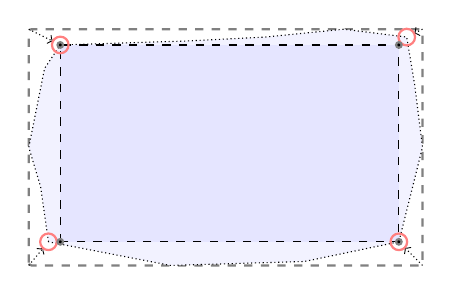
\begin{tikzpicture}[scale=1]
		
		%		
		\coordinate (P1) at (0,0);
		\coordinate (P2) at (0,3);
		\coordinate (P3) at (5,3);
		\coordinate (P4) at (5,0);
		
		\coordinate (C1) at (0.25,0.3);
		\coordinate (C2) at (0.4,2.8);
		\coordinate (C3) at (4.8,2.9);
		\coordinate (C4) at (4.7,0.3);
		
		
		\draw[thick,dashed,rounded corners = 1pt, gray] (P1) -- (P2) -- (P3) -- (P4) -- (P1) -- cycle;
		
		% L,T,R,B
		\draw[densely dotted, fill=blue!5] 
		(0.25,0.3) -- (0.15,1) --  (0,1.5) -- (0.2,2.5) -- (0.4,2.8) -- 
		(2,2.85)  -- (3,2.9) -- (4,3) -- (4.8,2.9) -- (4.9,2.3) --  (5,1.5) -- 
		(4.7,0.3) -- (3.5,0.05) -- (1.8,0) -- 
		cycle;
		
		\draw[->,densely dotted,black,shorten >=.1cm] (P1) -- (C1);
		\draw[->,densely dotted,black,shorten >=.1cm] (P2) -- (C2);
		\draw[->,densely dotted,black,shorten >=.1cm] (P3) -- (C3);
		\draw[->,densely dotted,black,shorten >=.1cm] (P4) -- (C4);
		
		
		% the inner rect
		\def\innerRect{
			(0.4,0.3) -- (0.4,2.8)  -- (4.7,2.8) -- (4.7,0.3) -- cycle
		}
		%		\draw[thick,dashed,rounded corners = 1pt, gray] \innerRect;
		%		\runeshade{dashed}{blue!10}{white} \innerRect;
		\draw[dashed, fill=blue!10] \innerRect;
		
		
		\draw[thick, color=red!50](C1) circle[radius = 3pt];
		\draw[thick, color=red!50](C2) circle[radius = 3pt];
		\draw[thick, color=red!50](C3) circle[radius = 3pt];
		\draw[thick, color=red!50](C4) circle[radius = 3pt];
		%
		\draw[thick, color=black!50, fill=black](0.4,0.3) circle[radius = 1pt];
		\draw[thick, color=black!50, fill=black](0.4,2.8) circle[radius = 1pt];
		\draw[thick, color=black!50, fill=black](4.7,2.8) circle[radius = 1pt];
		\draw[thick, color=black!50, fill=black](4.7,0.3) circle[radius = 1pt];
		%
		
		\end{tikzpicture}
		\caption{\small Fitting the input space: from the maximum device-aligned rectangle span of the input points (outer rectangle), inner rectangle corner candidates are identified (red circles) and the final fit (inner rectangle) equals the maximization of a rectangle within the space spanned by these candidates.}
		\label{fig:2dRectFit}
	\end{center}
\end{figure}

%Each corner of this rectangle will be  "ideal" in the sense that they would be true representations of the input space corners, were it not for the expected crooked corners. 
To produce this rectangle fit, the maximum top, right, bottom and left components are first identified from the full set of input points. This initially identifies both the location and the maximum possible dimensions of the input, corresponding to the outer rectangle in figure \ref{fig:2dRectFit}. To reach the desired smaller fit, a more appropriate set of corners is identified by, for each corner, picking the nearest neighbor from the full set of input points, i.e. the input point with shortest distance. The input space is then defined by the maximization of a rectangle within the space spanned by these new corner points. 
%To ensure a proper callibration, the end result is presented to the user as a transparent overlay that allows for easy visual verification, as shown in figure ??????.

We note that the orientation of this fitted rectangle is implicit. That is, the rectangle has sides top, bottom, left and right, as seen from the viewpoint of the user that provided the input. We will adopt these names to describe orientations, which will be relevant later on.


\subsubsection{Off-screen input plane}

The derivation of the device plane in off-screen space will be performed by the fitting of a set of spatial points, each assumed to be in close proximity to the plane spanned by the device. These points are in fact already available to us: in the previous derivation of the on-screen rectangle, pairings between on-screen and off-screen points were done. Hence, the fitting data is implicitly available as a set of  spatial tracking data points that should align closely with some plane (again, not perfectly due to factors such as tracking noise).% and the spatial corners of the on-screen plane.

%\fn{Technically each pairing instantiated at the availability of a new tracking point with the most recent on-screen input location. This makes each pairing unique, because the tracking device is the limiting factor (due the lower frame ratio of approximately 20 to 30 frames per second.)}. 
 
\paragraph{Geometrical view of the fitting}

To fit a plane to the set of spatial points, we will approach this as an optimization problem with some error to minimize. An intuitive choice would be attempting to express the sum of all projection distances to the plane of choice and then use calculus to differentiate and solve for the minimum. However, this would involve calculating Euclidean distances in multi-dimensional space, which cannot easily be differentiated. 

To identify an alternative fitting strategy, we will give some thought to the geometry of the tracking points. In particular, if we assume that the tracking noise is Gaussian with the mean spanning a plane, we get geometry such as  that shown in figure \ref{fig:fitSinePlane}. 

%The first step in processing this set of spatial data points is to derive some plane by which they are assumed to fluctuate around, as illustrated in figure \ref{fig:fitSinePlane}. This task is challenged by the degree of inherent imprecision in the spatial tracking mechanism, a factor that is expected to be present but minimal. 

\begin{figure}[!h]
	\begin{center}	
		\begin{tikzpicture}[x={(290:0.8cm)}, y={(-10:1cm)}, z={(0,1cm)}, scale=1.2,
		%		\begin{tikzpicture}[x={(-160:1cm)}, y={(-20:1cm)}, z={(0,1cm)}, scale=1.2,
		%		\begin{tikzpicture}[x={(-180:1cm)}, y={(180:0.8cm)}, z={(0,1cm)}, scale=1.2,
		plane max z=3]
		
		\node[text width=0.2cm,gray] at (4,-0.3,0) {\small x};
		\node[text width=0.2cm,gray] at (-0.3,4,0) {\small y};
		\node[text width=0.2cm,gray] at (0,-0.25,4) {\small z};
		
		\draw[->] (0,0,0) -- (4,0,0);
		\draw[->] (0,0,0) -- (0,4,0);
		\draw[->] (0,0,0) -- (0,0,4);
		
		\definePlaneByEquation{myplane}{1}{1}{1}{3}
		\drawPlane[thick,fill=blue!4]{myplane}
		
		\begin{loopTabbedCsv}[data/sinePlaneFitPoints.csv]{sinePlaneFitPoints}{\x=x,\y=y,\z=z}
		\definePointByXYZ{p51}{\x}{\y}{\z};
		\draw[color=red!50](p51) circle[radius = 1pt];
		\projectPointToPlane{projp51}{p51}{myplane}
		\fill[color=black!80](projp51) circle [radius=1pt];
		\draw[->, shorten <= 1pt, shorten >= 1pt, color = gray!60](p51) -- (projp51);
		\end{loopTabbedCsv}
		
		
		\end{tikzpicture}
		\caption{A sequence of spatial points, generated by departing a sine curve along the the normal of the easily comprehensible example plane  $x + y + z = 3$. The departure magnitude is defined by sampling from a Gaussian distribution with zero mean. Given a set of these points, this plane could therefore be considered an appropriate fitting.}
		\label{fig:fitSinePlane}
	\end{center}
\end{figure}





Additional insight is obtained when viewing this example in profile, as shown in figure \ref{fig:fitSinePlane2}. From this, we see that with Gaussian noise we will see equal fluctuations  on either side of the plane fit. In addition, choosing to project along a single axis should not change the plane fit, since the result is merely a scaling of the projection lengths, as illustrated in figure \ref{fig:fitSinePlaneAlongZ}. The geometric relations of this observation are further illuminated in figure  \ref{fig:axisProjectionIsTriangle}, which shows that this approach scales each plane-orthogonal projection length by the inverse of the angle between the plane's normal and the projection axis (i.e. a constant factor).




\begin{figure}[!h]
	\begin{center}	
		%		\begin{tikzpicture}[x={(290:0.8cm)}, y={(-10:1cm)}, z={(0,1cm)}, scale=1.2,
		%		\begin{tikzpicture}[x={(-160:1cm)}, y={(-20:1cm)}, z={(0,1cm)}, scale=1.2,
		\begin{tikzpicture}[x={(-180:1cm)}, y={(180:0.8cm)}, z={(0,1cm)}, scale=1.2,
		plane max z=3]
		%		\node[text width=0.2cm,gray] at (4,-0.3,0) {\small x};
		%		\node[text width=0.2cm,gray] at (-0.3,4,0) {\small y};
		\node[text width=0.2cm,gray] at (0,-0.25,4) {\small z};
		
		\draw[->] (0,0,0) -- (4,0,0);
		\draw[->] (0,0,0) -- (0,4,0);
		\draw[->] (0,0,0) -- (0,0,4);
		
		
		
		\definePlaneByEquation{myplane}{1}{1}{1}{3}
		\drawPlane[thick,fill=blue!4]{myplane}
		
		%		\input{data/sinePlaneFitPoints}
		
%\csvloop{
%	file=data/sinePlaneFitPoints.csv,
%%	no head,
%	head to column names,
%	command={
%			\definePointByXYZ{p51}{\x}{\y}{\z};
%			\draw[color=red!50](p51) circle[radius = 1pt];
%			\projectPointToPlane{projp51}{p51}{myplane}
%			\fill[color=black!80](projp51) circle [radius=1pt];
%			\draw[->, shorten <= 1pt, shorten >= 1pt, color = gray!60](p51) -- (projp51);
%	},
%	late after line=,
%	late after last line=,
%}		

		\begin{loopTabbedCsv}[data/sinePlaneFitPoints.csv]{sinePlaneFitPoints}{\x=x,\y=y,\z=z}
			\definePointByXYZ{p51}{\x}{\y}{\z};
			\draw[color=red!50](p51) circle[radius = 1pt];
			\projectPointToPlane{projp51}{p51}{myplane}
			\fill[color=black!80](projp51) circle [radius=1pt];
			\draw[->, shorten <= 1pt, shorten >= 1pt, color = gray!60](p51) -- (projp51);
		\end{loopTabbedCsv}
		
		
		
		\end{tikzpicture}
		\caption{A profile view of the example plane with orthogonal projections.}
		\label{fig:fitSinePlane2}
	\end{center}
\end{figure}

\begin{figure}[!h]
	\begin{center}	
		%		\begin{tikzpicture}[x={(290:0.8cm)}, y={(-10:1cm)}, z={(0,1cm)}, scale=1.2,
		%		\begin{tikzpicture}[x={(-160:1cm)}, y={(-20:1cm)}, z={(0,1cm)}, scale=1.2,
		\begin{tikzpicture}[x={(-180:1cm)}, y={(180:0.8cm)}, z={(0,1cm)}, scale=1.2,
		plane max z=3]
		%		\node[text width=0.2cm,gray] at (4,-0.3,0) {\small x};
		%		\node[text width=0.2cm,gray] at (-0.3,4,0) {\small y};
		\node[text width=0.2cm,gray] at (0,-0.25,4) {\small z};
		
		\draw[->] (0,0,0) -- (4,0,0);
		\draw[->] (0,0,0) -- (0,4,0);
		\draw[->] (0,0,0) -- (0,0,4);
		
		\definePlaneByEquation{myplane}{1}{1}{1}{3}
		\drawPlane[thick,fill=blue!4]{myplane}
		
		%		\input{data/sinePlaneFitPointsAlongZ}
		
		\begin{loopTabbedCsv}[data/sinePlaneFitPoints.csv]{sinePlaneFitPoints}{\x=x,\y=y,\z=z}
		\definePointByXYZ{p51}{\x}{\y}{\z};
		\draw[color=red!50](p51) circle[radius = 1pt];
		\projectPointToPlaneAlongZ{projp51}{p51}{myplane}
		\fill[color=black!80](projp51) circle [radius=1pt];
		\draw[->, shorten <= 1pt, shorten >= 1pt, color = gray!60](p51) -- (projp51);
		
		\projectPointToPlane{projp51}{p51}{myplane}
		\fill[color=black!80](projp51) circle [radius=1pt];
		\draw[->, dotted, shorten <= 1pt, shorten >= 1pt, color = gray](p51) -- (projp51);
		\end{loopTabbedCsv}
		
		
		\end{tikzpicture}
		\caption{Projecting points to the plane along the z-axis, with previously shown projections normal to the plane shown as dotted lines. With a 45 degree plane, each projection length is now $\i1/{sin (45\degree)} = \sqrt{2}$ that of the orthogonal projection. While the z-aligned projections obviously obfuscate the original sine curve, the plane fitting remains unaffected, which is our sole interest.}
		\label{fig:fitSinePlaneAlongZ}
	\end{center}
\end{figure}

\begin{figure}[!h]
	\begin{center}
		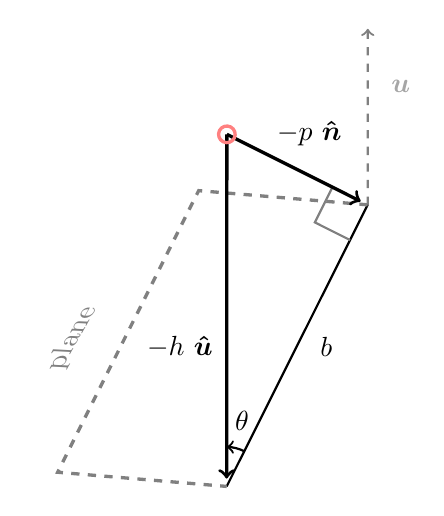
\begin{tikzpicture}
		
		
		%	\draw[->] (0,0,0) -- (4,0,0);
		%	\draw[->] (0,0,0) -- (0,4,0);
		%	\draw[->] (0,0,0) -- (0,0,4);
		%	
		%	\definePlaneByEquation{myplane}{1}{1}{1}{3}
		%	\drawPlane[thick,fill=blue!4]{myplane}
		
		%	\drawPlane[thick,fill=blue!4]{myplane}
		
		%	\newcommand{\pOne}{(0,2)}
		
		\begin{scope}[rotate=63.4
		]
		
		\coordinate (P1) at (0,0);
		\coordinate (P2) at (-4,0);
		\coordinate (P23) at (-2, 2);
		\coordinate (P3) at (0,2);
		
		\coordinate (U) at (2,1);				
		
		\coordinate (U1) at (0,0.5);				
		\coordinate (U2) at (-0.5,0.5);				
		\coordinate (U3) at (-0.5,0);				
		
		
		\begin{scope}[shift={(-0.8,2)}]
		
		\coordinate (Q1) at (0,0);
		\coordinate (Q2) at (-4,0);
		\coordinate (Q3) at (0,2);
		
		%					\shade[top color=blue!13!white,opacity=0.5] (-1,0) (P1) -- (P2) -- (Q2) -- (Q1) -- cycle;
		
		%				\IFBUILDSTART
		%				\shade[top color=blue!13!white,opacity=0.5] (P1) -- (P2) -- (P3) -- cycle;
		%				\IFBUILDEND			
		%					
		\end{scope}
		
		
		\drawWithBuildOption{white}{top color=\themeColorLight} (P1) -- (P2) -- (P3) -- cycle;
%		\draw[white,top color=\themeColorLight] (P1) -- (P2) -- (P3) -- cycle;
		
		\pic [thick, draw, ->, "$\theta$", angle eccentricity=1.7] {angle = P1--P2--P3};
		
		\draw[->,thick,dashed,rounded corners = 1pt, gray] (P1) -- (U);
		
		\draw[thick,rounded corners = 1pt, black] (P1) -- (P2);
		
		\draw[very thick,dashed,gray] (P1) -- (Q1) -- (Q2) -- (P2);
		
		\draw[thick,gray] (U1) -- (U2) -- (U3);
		
		%				\draw[->,very thick,black] (P2) -- (P23);
		\draw[->,very thick,black,shorten >=.1cm] (P3) -- (P2);
		\draw[->,very thick,black,shorten >=.1cm] (P3) -- (P1);
		
		\draw[very thick, color=red!50](P3) circle[radius = 3pt];
		
		\end{scope}
		
		\node[text width=0.4cm,gray, rotate=87,yslant=-0.5] at (-3.87,-1.9) {plane};
		
		\node[text width=0.2cm,gray!70] at (0.4,1.5) {$\b{u}$};
		\node[text width=0.3cm,black] at (-1,0.9) {$ - p \ \b{\hat{n}}$};
		%			\node[text width=0.2cm,black] at (-1.3,2) {$$};
		\node[text width=0.2cm,black] at (-0.5,-1.8) {$b$};
		\node[text width=0.4cm,black] at (-2.6,-1.8) {$ - h \  \b{\hat{u}}$};
		%			\node[text width=0.2cm,black] at (-3.2,1.8) {$h$};
		%			\node[text width=0.2cm,black] at (-3.2,-1.3) {$\hat{k}$};
		
		\end{tikzpicture}
		\caption{A closer examination of the alternative (axis-aligned) projection: given plane-orthogonal projection length $p$, the alternative axis-aligned projection length $h$ will be equal to the hypotenuse of the right triangle formed by $p$ and the planar distance $b$ between the two projections. Hence,  $ h= \ifrac{p}{\sin\theta} $ (since $\sin \theta = \i{p}/h$), which means that the axis-aligned projection scales  $p$ by $\infty > (\sin\theta)^{-1} >= 1$. }
		\label{fig:axisProjectionIsTriangle}
	\end{center}
\end{figure}

Overall, choosing the axis-aligned projection allows for effectively eliminating the complexity of multiple dimensions, at the cost of some information loss. But the loss is irrelevant, since we only care about the ratio between the aggregation of projection distances on either side of the plane, which remain unaffected. Hence, under the assumption of Gaussian noise, this projection method is therefore appropriate for performing the plane fit.

%\subsubsection{{Plane proximity }
\subsubsubsection{Numerical precision for extreme angles}

Since $\theta \approx 0 $ is theoretically possible  for planes close to parallel with the projection axis, that would result in large projection lengths since
$$
\lim_{\theta \to 0 } h  = \frac{p}{\sin \theta} = \infty
$$
. It would be natural to wonder if this could have any implications on numerical precision. While such conditions must necessarily increase the projection distances greatly, is should be irrelevant since we are solving for the zero-gradient of the derivative, rather than searching the solution space directly. Hence, we do not need to worry.   





%Either way, and for the sake of the example, even for an unlikely case of observing $\theta = 0.1\degree$ and $p=1000$ we would get
%$$
%h = \frac{1000}{\sin(0.1\degree) } \approx 5.730 \times 10^5
%$$
%which, with an upper limit of more than $10^{308}$ on the data type employed\fn{.NET \href{http://msdn.microsoft.com/en-us/library/system.double.maxvalue}{\ti{double}}}, would allow for summing up at least
%$$ i_{max} = \frac{10^{308}}{5.730 \times 10^5} \approx 10^{302}$$
%such data point projections and still be well within the numerical boundaries. Since in the solution we expect the plane calibration process to last no more than 10 seconds, each yielding 120 tracked points, we will assume that there is plenty of room for numerical operations despite extended projection distances. 
%
\subsubsubsection{Fitting the off-screen plane}

With a fitting strategy and confidence in the method in place, we may now proceed by finding an expression for the derivative of the aggregated projection lengths, which we will choose to perform along the $z$ axis. 
Starting off, we observe that given the scalar equation for a plane $$ ax + by +  cz = d$$, we can express any single component as a linear combination of the other two. For instance, we could express the z-component as a function of the x- and y-component 
$$ z = \(\frac{-a}{c}\)x + \(\frac{-b}{c}\)y + \frac{d}{c} $$
, or more simply 
$$ z= \alpha x + \beta y + \delta $$
to lighten the notation. Our plane fitting error will therefore be defined as the sum of squared deviations 

\begin{eq}
	E(\alpha,\beta,\delta) 
	& = \sum_i \( z_i - (\alpha x_i + \beta y_i + \delta) \)^2
	%	\\ 
	%	& = \sum_i \( z_i - ax_i - by_i + c \)^2
\end{eq}
in which it is straightforward to see that each summation element will have partial derivatives

\begin{eq}
	\frac{\partial E}{\partial \alpha} 
	& = 2x(\alpha x + \beta y + \delta - z)
	\\
	\frac{\partial E}{\partial \beta} 
	& = 2y(ax + by + c - z)
	\\
	\frac{\partial E}{\partial \delta} 
	& = 2(\alpha x + \beta y + \delta - z)
\end{eq}
that are all linear in the input variables. Setting these to zero

\begin{eq}
	\frac{\partial E}{\partial \alpha} = 0 & \ \lra \ 2x(\alpha x + \beta y + \delta - z) = 0
	\\ 
	& \ \lra \ \alpha x^2 + \beta xy + x \delta \ \ \ \ \ \ = xz 
	\\
	\\
	\frac{\partial E}{\partial \beta} = 0  &  \ \lra \ \alpha x + \beta y^2 + \delta y = yz
	\\
	\\
	\frac{\partial E}{\partial \delta} = 0 & \ \lra \ \alpha x + \beta y + \delta = z
\end{eq}
\\\
makes it clear that the minimum is obtained through a linear system of three equations with three unknowns. Thus, we may sum up the zero derivative of the error in the compact matrix form
\begin{eq}
	AX & = b
	\\ & \uda \\
	\( \sum_i 	\m{
		x^2 & xy & x \\
		xy & y^2 & y \\
		x & y & 1		
	} \)
	\m{\alpha \\ \beta \\ \delta}
	& = 
	\sum_i \m{ xz \\ yz \\ z }
\end{eq}
\\\
which has the simple solution  
\begin{eq}
	X & = A^{-1}b
	\\ & \uda \\
	\m{\alpha \\ \beta \\ \delta}
	& = 
	\( \sum_i 	\m{
		x^2 & xy & x \\
		xy & y^2 & y \\
		x & y & 1		
	} \)^{-1}
	\sum_i \m{ xz \\ yz \\ z }
\end{eq}
\\\
%, as is easily seen in extremes such as $x=y$, $x+y=-1$, $x=0$ or $y=0$
provided that the matrix  $A$ is invertible. To argue that this will be the case, we note that $A$ will surely not have full rank in the case of a pure linear relationship such as $x=y$ (as clearly seen from the first two rows of $A$). However, the geometric interpretation of this, a straight line formed by the $x$ and $y$ components of the tracking points, allows us to quickly dismiss this as a special case that is unlikely to occur, since the inherent noise in the tracking data makes the probability of obtaining exact linear correlations infinitesimally small. 

Hence, with $A$ assumed invertible and the ability to solve directly for the solution component vector $$[\alpha, \beta, \delta]^T$$, our fitted plane $$ax+by+cz=d$$ will then be described by $$-\alpha x - \beta y + z = \delta$$, where $c=1$ because we were solving for $z$, i.e. implicitly using a coefficient of one. 

\subsubsection{Off-screen rectangle fitting}

As with the processing of the on-screen data, we'll also need to fit a rectangle to the off-screen points, in order to eventually be able to precisely correlate the two spaces. However, the former on-screen case was trivial because the location and scale of the on-screen rectangle was implicit (through the minimum and maximum values of the horizontal and vertical input components). For the off-screen rectangle however, this may be located anywhere in the (previously derived) spatial plane fit and have any scale, orientation and side ratio. And again, the noisy tracking  points are unlikely to form a perfect rectangle. 

%%%%%%%%%%%%%%%%%%%%%%%%%
%\subsubsection{Deriving and correlating orientations}
%
%To successfully relate the input spaces we'll need to deduce and correlate the device orientations relative to the user. That is, ensure an identity bijection between instances of 
%$$\s{S} = \{T, B, L, R\}$$
%that allows us to describe the set of sides $$\{top, bottom, left, right\}$$, of which we have two, since the on-screen and off-screen points each give rise to a rectangle. Henceforth we will distinct the two, with the prior referenced as $\s{D}$  (rectangle of the display) and the latter as $\s{T}$ (rectangle of the tracker), both being dictionaries indexed by $\s{S}$ with values corresponding to the set of points identified as belonging to the given key (i.e. $\s{T}_L$ will designate the subset of points captured from the tracker that are identified as belonging to the \ti{left} side of the off-screen rectangle).
%
%%%%%%%%%%%%%%%%%%%%%

% $\mathbbm{S}_\ti{on-screen}$ and $\mathbbm{S}_\ti{off-screen}$, where both are instances of 

%$$\mathbbm{S} = \{top, bottom, left, right\}$$


%. To do so, we'll need to reference the corners
%\begin{eq}
%	\mathbbm{C} = \{ \ & \{top,left\}, && \{top,right\}, & \\
%		& \{bottom,left\}, && \{bottom,right\} \ \} & 
%\end{eq}
%of the rectangle and will henceforth use the shorthand notations $ \{ \mathbbm{C}_{TL}, \mathbbm{C}_{TB},\s{C}_{BL},\s{C}_{BR} \} $ to reference corners, i.e. single elements of $\mathbbm{C}$.


%\subsubsection{On-screen orientations}
%
%For the on-screen points, $\mathbbm{S}_\ti{on-screen}$ will be implicit through the min-max values of its vertical and horisontal components.

% \fn{Specifically, the implementation uses a WinRT \ti{Canvas} component that places the origo in the top-left corner of the display by default and uses natural number components only to specify locations in the visible part of the display}. Hence, with already known on-screen rectangle corners and each of these paired with a corresponding off-screen point $\b{p_c}$, we are already given the four prime candidates for the off-screen rectangle corners. 


\subsubsection{Estimating off-screen rectangle corners}

To derive the rectangle, we'll first identify the expected location of the corners. We again exploit that we have previously identified the corners of the on-screen input space. Since each of these is paired with a tracking point, the  four spatial corner locations  are already available to us. We will refer to these spatial corner points as the \ti{corner candidates}.

\def\smoothCount{3}
Although we could proceed immediately with these candidates, we will take into account that they are originate from a noisy stream of data. We should we care? Because minor inaccuracies could have a large impact on the solution, since the effects of a poorly calibrated plane will be amplified in subsequent spatial projections onto it (or so we assume). Hence, seeking a better approximation of the true locations may be justified and is easily achieved by averaging over a few neighboring frames, rather than settling on single ones. 

The question is then, how many neighbors to include? An intuitive choice is to include frames that co-occur at the time the user's finger was located at the corner, making time our indicator of co-occurrence.  So, rather than simply settling on the initial single corner candidates,  these will be redefined by seeking out  $m$ neighboring tracked coordinates, using their individual capture times relative to the candidate corner as distance measure. 

We will choose $m$, based on the assumption that a spatial point is received from the tracker every 
$$ (30\  \ifrac{\text{frame}}{\text{s} })^{-1} \approx 33.3 \ \text{ms}$$ 
and that the input (finger) will not move significantly in the corner within $100 $ milliseconds. We therefore choose 
$$\frac{100 \ \text{ms}}{33.3 \ \text{ms}} > 3  = m $$
as the number of spatial points to average over, meaning that we'll seek out $m-1=2$ neighbors. Again, these points need to co-occur within a time span of $100 \ \text{ms}$, a check that will be enforced in the implementation. 

%Additionally we would like points closer in capture time to the candidate corner point to have greater influence on the averaged corner, compared to those farther away. We will achieve this by incorporating weights, one for each point $1 \ge i \ge m$ as 
%
%
%%from the capture time of the corner point candidate $\b{p_c}$. The $m$ smoothing points in $\s{N}_c$ will then "vote" to determine the final "smoothed" location $\b{\hat{p}_{c}}$  as a weighted sum of the point components
%
%%
%% In numbers, it is verified that the movement does not exceed $3 \ \ifrac{\text{cm}}{\text{s}}$ for each $\s{N_c}$, which corresponds to a maximum possible travel distance of $(3\ \ifrac{\text{cm}}{\text{s}})(25 \text{ms}) =  0.75 \text{mm} $ and assumed to be a negligible factor}. 
%
%
%\begin{eq}
%	w_i 
%%	& = 1 - \frac{d_i (m-1)}{D }  
%	& = \frac{1}{m } \(1 - \frac{d_i }{D }  \)
%	%		&& \parbox{10em}{for each corner $c \in \s{C}$} 		
%\end{eq}
%where $d_i$ is the time distance of point $i$ from the candidate corner and $D$ 
%
%\begin{eq}
%	 \sum_{i=1}^m d_i  & = D
% 	\\ & \uda \\ 
%	 \sum_{i=1}^m \frac{d_i}{D}
%	 & = 1  
%\end{eq}
%is the aggregation of all these distances, such that the sum of all weights is
%\begin{eq}
%	\sum_{i=1}^m w_i
%	& = \sum_{i=1}^m  \( \frac{1}{m} \) \(1 - \frac{d_i }{D }  \) 
%	\\
%	& =  \frac{1}{m} - (m-1)\sum_{i=1}^m \frac{d_i}{D } 
%	\\
%	& = m - (m-1)(1) 
%	\\
%	& = 1 
%\end{eq}
%, which confirms that the choice of weights add up as expected. Note, this definition achieves the desired inverse relationship, that gives greater weight to points closer to the candidate point. 
%
%Thus, given a set of $m$ corner points $\{ \b{p_1},\dots,\b{p_m}  \}$ (that includes the corner candidate itself),  the final corner approximation $\b{\hat{p}}$ is defined as the weighted sum 
%
%
%\begin{eq}
%	\b{\hat{p}} 
%	& = \sum_{i=1}^m \b{p_i}  w_i 
%	\\
%	& = \sum_{i=1}^m \b{p_i}  \(1 - \frac{d_i (m-1)}{D} \) 
%	%		&& \parbox{10em}{for each corner $c \in \s{C}$} 		
%\end{eq}
%which is assumed to be a numerical optimization of the original candidate.
%%%%%%%%%%%%%%%%%%%%%%%%%%%%%%

 
% %$D$ in $\s{N}_c$, 
%\begin{eq}
%	w_i & = \frac{d_i}{D_c}  
%	%	&& \parbox{10em}{} \\
%	%	& \rightarrow \ \sum_i w_i = 1		
%\end{eq}
%and $D_c = \sum_i d_i$, such that $\sum_i w_i = 1$ for each corner $c$. 

%\fn{In addition, the implementation verifies that the frame rate holds, such that the timespan of $\s{N_c}$ does not exceed 25 milliseconds.}


\subsubsection{Deriving off-screen rectangle}

Having settled on four spatial locations that combined should closely resemble a rectangle, we proceed to align them so that they do in fact correspond to the formal structure of a rectangle. 

\subsubsubsection{Constraints of a true rectangle}
%\b{\hat{p}}
While we could easily just form lines between the chosen corner locations, the end result would not be purely rectangular, but a trapezium (i.e. a quadrilateral with no parallel).  Hence, we will need to somehow relate all points concurrently, while  matching them against constraints that capture the desired structure of a rectangle.

To define these constraints, we observe that rectangle lines are all related. The pair of lines that run parallel (top and bottom) will share the normal vector $\b{n}$, but different offsets $c_T$ and $c_B$. The vertical pair of lines (left and right) are both orthogonal to the horizontal ones. Each too have individual offsets $c_L$ and $c_R$, and share the perpendicular normal $\b{n^\perp} = [-n_y, n_x]^T$. Hence, the quantities needed for describing the rectangle are offsets $\b{c} = \m{c_T, c_B, c_L, c_R }^T $ and vector $\b{n}$ (which is normal to the top and bottom lines). 

\subsubsubsection{Dimensionality reduction}

Since the derived estimations of the rectangle corners should theoretically all  be closely aligned with the already derived off-screen plane, we may as well simplify by projecting them directly (orthogonally) onto this plane. Hence, a dimensionality reduction will be performed to completely rid the dimension that is orthogonal to the plane, by finding a new two-dimensional coordinate system that represents the plane. This idea is exemplified in figure \ref{fig:planeProjectNoFit1} and \ref{fig:planeProjectNoFit2}, which show two different viewpoints. 

In more detail, suppose we have a  set  $ \s{\hat{P}}$ of three-dimensional points centered around some mean
$$ \b{\phi} =\setSize{\s{\hat{P}}}^{-1}  \sum_{\b{\hat{p}}}^{\s{\hat{P}}} \b{\hat{p}} $$
, where we use the "hat" notation to indicate a vector of three dimensions. We then accomplish the reduction through a number of steps. First, the spatial center $\b{\phi}$ is determined and all points are projected onto the (previously derived) plane using simple geometry. Next, a spatial unit vector $\b{\hat{i}}$ of the new coordinate system is generated by crossing the plane normal with the unit vector of the x-axis. Since this will be orthogonal to the plane normal, it will be in the plane. A second unit vector $\b{\hat{j}}$ is then produced by crossing the first unit vector with the plane's normal. This second unit vector will then be orthogonal to both the first unit vector and the plane normal. With two perpendicular unit vectors, any spatial point $\b{\hat{p}}$ in the plane may then be converted to its equivalent $\b{{p}}$ in new two-dimensional system by simple scalar projections. That is, $\b{{p}}$ will have components 
 $$ \b{p} = \m{ \  \b{\hat{i}} \cdot  (\b{\hat{p}}-\b{\phi}) \\ \ \b{\hat{j}} \cdot  (\b{\hat{p}}-\b{\phi}) \  } $$
which is the dot product of each spatial unit vector with  $\b{\hat{p}}-\b{\phi}$ (the vector going from the center $\b{\phi}$ and to the point of interest). This process is illustrated in figure 	\ref{fig:dimRedictNoFit}.
 


\begin{figure}[!h]
	\begin{center}
		\planeProjectNoFit{-180:1cm}{0:0.8cm}{0,1cm}{}
		\caption{Exaggerated for the purpose of the example: this shows the effect of a projecting the corners of a horizontal rectangle onto a 45 degree plane in the positive octant. The mean of the projections is shown as a circle to help illuminate the geometry.} %, as well as the derived center $\b{\phi}$
		\label{fig:planeProjectNoFit1}
	\end{center}
\end{figure}

\begin{figure}[!h]
\begin{center}
	%	\captionof{table}{Survival for all decks.}
	\begin{tabular}[!ht]{C{0.5\linewidth}C{0.5\linewidth}} 
%		\begin{figure}[!h]
%			%			\planeProjectSpatialExample{270:0.8cm}{0:1cm}{2.25,1cm}
%		\end{figure}
%		&
%		\begin{figure}[!h]
%			%			\planeProjectSpatialExample{270:0.8cm}{0:1cm}{2.25,1cm}
%		\end{figure}

%		\begin{figure}[!h]
				\planePointProjectExample{290:0.8cm}{-10:1cm}{0,1cm}{scale=0.8}%{270:0.8cm}		
%	\end{figure}
	&
\planeProjectNoFit{270:0.8cm}{0:1cm}{2.25,1cm}{scale=0.6}	
%\planeProjectSpatialExample{270:0.8cm}{0:1cm}{2.25,1cm}
	\end{tabular}
	\caption{Additional views of the previous example, with the right figure showing a top-down view of the horizontal plane at (z-axis) height that intersects exactly with the plane (which makes it appear as a line). In practice, we do not expect such extreme fitting to occur, the simplicity of the geometry is chosen to aid the reader's comprehension of the projections.}
	\label{fig:planeProjectNoFit2}
\end{center}
\end{figure}

%
%\begin{figure}[!h]
%	\begin{center}
%%		\begin{minipage}{.5\textwidth}
%				\planePointProjectExample{290:0.8cm}{-10:1cm}{0,1cm}{}%{270:0.8cm}{0:1cm}{2.25,1cm}
%%		\end{minipage}%
%%		\begin{minipage}{.5\textwidth}
%%			\planeProjectNoFit{270:0.8cm}{0:1cm}{2.25,1cm}
%%		\end{minipage}
%				\caption{Additional view of the previous example. }
%				\label{fig:planeProjectNoFit2}
%		
%	\end{center}
%\end{figure}


%		\plotPlanarRectFit{-1.5}{1.5}{-1.5}{1.5}{}
\begin{figure}[!h]
	\begin{center}
		\plotPlanarRectNoFit{-1.5}{1.5}{-1.5}{1.5}{} %, along with the derived $\b{\phi}$ in origo
		\caption{The result of converting the previous exaggerated example to a two-dimensional coordinate system. Fitting a rectangle to these two-dimensional points implicitly has a spatial equivalent if given two spatial unit vectors. Note a color convention has been introduced for indicating rectangle orientations (as they appear here), which will be used consistently henceforth.}
		\label{fig:dimRedictNoFit}
	\end{center}
\end{figure}

In addition, it is straightforward to convert any point $\b{p}$ in the two-dimensional coordinate system back to the spatial location in the plane. This is easily achieved by 
\begin{eqRef}\label{eq:convertBack}
\b{\hat{p}} = \b{\phi} +  {p}_x \b{\hat{i}} + {p}_y \b{\hat{j}}  
\end{eqRef}
, that is, scaling the unit vectors by the components of $\b{{p}} $ and offset by the spatial center $\b{\phi}$. Hence, if we are able to derive a rectangle from the points in the new two-dimensional coordinate system, we have implicitly derived a rectangle in the spatial off-screen plane, which is our goal.


\subsubsubsection{Formulating the optimization problem}

%Having determined $\s{T}$ and its four sets of points, we'll need to process these and derive the rectangular shape of the off-screen input space. Obviously, if were proceed by fitting straight lines to each of these sets independently, we would not end up with a rectangle, but a trapezium (), as shown in figure ???. Hence, we will need to relate the points concurrently.

In broad terms, we will accomplish the fitting by attempting to minimize residuals\fn{In more detail, we build upon an approach for fitting parallel lines (section 6.7 of \cite{SciCom}), although modified for our more complex case of fitting a rectangle.}. We note that, given a point $\b{p}$ in some plane, we may describe its distance to a line that has orthogonal vector $\b{n}$ and offset $c$ by the residual

% the  given a point $\b{p}$, a vector $\b{n}$ and value $c

% we note that we may describe a side of the eventual rectangle by any combination of parameters for which the output of the residual function 
\begin{eqRef}\label{eq:eqLine}
	r(\b{p}, \b{n}, c) = \b{n} \cdot \b{p}  + c 
\end{eqRef}
. That is, the residual equals the shortest Euclidean distance to the line, which will be zero if it is exactly on the line. So, if we were to fit a line to a set of points $\s{P}$, we could define the squared residual error
 % (in which case (\ref{eq:eqLine}) simply becomes the equation of a line)
\begin{eq}
	E_\text{line} ( \b{n}, c,  \s{P}) & = 	\sum_{\b{p}}^{\s{P}} \( r(\b{p}, \b{n}, c) \)^2 
	%	\underset{\b{n},c}{\text{minimize}} 
	%	\\
	%	& = 	\underset{\b{n},c}{\text{minimize}} \sum_{\b{p}}^{\s{P}}  \( \b{n} \cdot \b{p} + c \)	
\end{eq}
which is minimized for some choice of $\b{n}$ and $c$.

Thus, is we had four sets of points, one for each side of an approximate rectangle, we could align these to the formal definition of a (true) rectangle by minimizing the residuals for each side as

\begin{eq}
	E_{\text{rect}} \( \b{n}, \b{c},  \s{P}_T,\s{P}_B,\s{P}_L,\s{P}_R \)  
	= & \sum^{\{T,B,L,R\}}_{s}  {E_\text{line}(\cdots)} %r_p^2  
	\\
	= & \sum^{ \{ T,B \} }_{s} \ \sum_{\b{p}}^{\s{P}_s}  ( \b{n} \cdot \b{p} + c_s )^2 \ \ +  
	\\
	& \sum^{ \{ L,R \}  }_s \ \sum_{\b{p}}^{\s{P}_s}   ( \b{n^\perp} \cdot \b{p} + c_s )^2   
	\\
	>= & 0
\end{eq}
using shared inputs $\b{n}$ and $\b{c}$, the latter being the vector of all four offsets. We note the such four sets of points in the input  are already inferable, since we have  previously settled on the spatial location of each off-screen corner. 

Hence, the fitting of a rectangle may then be described as the minimization 
\begin{eqRef}\label{eq:of}
	%	\underset{\b{n},\b{c}}{\text{min}} \ E_{\text{rect}} 
	\arg \min_{\b{n},\b{c}} E_{\text{rect}} (\cdots) % (\s{P}_T,\s{P}_B,\s{P}_L,\s{P}_R)
%	=  \sum^{\vectorsize{\b{r}}}_{i=1} r_i^2 \)
\end{eqRef}
subject to 
\begin{eqRef}\label{eq:quadConstr}
	\norm{n} = 1
\end{eqRef}
%that implicitly avoids any trivial solution 
and the linear constraints 
\begin{eqRef}\label{eq:systemConstr}
	 \b{r}	 & = A\b{x}
%	\\  & \text{ \scalebox{1.4}{$\uda$} } \\ 
	\\  & \uda  \\ 
	\m{ 
		\b{r_T} \\ \b{r_B} \\ \b{r_L} \\ \b{r_R} \\ 
	}
	& = 
	\m{ 
		1 & 0 & 0 & 0 & T
		\\
		0 & 1 & 0 & 0 & B 
		\\
		0 & 0 & 1 & 0 & L  
		\\
		0 & 0 & 0 & 1 & R  
	} 
	%	\m{c_T \\ c_B \\ c_L \\ c_R \\ n_x \\ n_y }
	\m{\b{c} \\ \b{n} } 
%	\\  & \uda  \\ 
\\
	& = 
	\m{ 
		1 & 0 & 0 & 0 & \b{T_x} & \b{T_y} 
		\\
		0 & 1 & 0 & 0 & \b{B_x} & \b{B_y} 
		\\
		0 & 0 & 1 & 0 & \b{L_y} & -\b{L_x} 
		\\
		0 & 0 & 0 & 1 & \b{R_y} & -\b{R_x} 
	} 
	%	\m{c_T \\ c_B \\ c_L \\ c_R \\ n_x \\ n_y }
	\m{\b{c} \\ \b{n} } 
%	& 
%	= \m{ 
%		\b{r_T} \\ \b{r_B} \\ \b{r_L} \\ \b{r_R} \\ 
%	}
\end{eqRef}
that captures our parameterized definition of the rectangle structure in matrix notation. Here, we describe the tracking data through horizontally stacked matrices $\{T,B,L,R\}$, each being the vertical concatenation of an $x$ and $y$ column vector. Also, the vectors $\b{r}$ are the residuals of the points in the particular rectangle side (each identified by  subscript). To be explicit, if  we were to expand the former we would get the more verbose

\begin{eqRef}\label{eq:AExpanded}
%	\\  & \parbox{9em}{\small where, to lighten the notation, $\b{s_c}$ entries (left) are vectors of scalar $c$-components and $\b{r_s}$ entries (right) are vectors of residuals, both constrained to side $s \in \s{S} $} \\
%	\\  & \text{ \scalebox{1.4}{$\uda$} } \\
	\m{ 
		{r_T}_1 \\ {r_T}_2 \\ \vdots \\ 
		{r_B}_1 \\ {r_B}_2 \\ \vdots \\
		{r_L}_1 \\ {r_L}_2 \\ \vdots \\ 
		{r_R}_1 \\ {r_R}_2 \\ \vdots  
	} 
	& = 
	\m{ 
		1 & 0 & 0 & 0 & {T_1}_x & {T_1}_y 
		\\
		1 & 0 & 0 & 0 & {T_2}_x & {T_2}_y 
		\\
		\vdots & \vdots & \vdots & \vdots & \vdots & \vdots 
		\\
		0 & 1 & 0 & 0 & {B_1}_x & {B_1}_y 
		\\
		0 & 1 & 0 & 0 & {B_2}_x & {B_2}_y 
		\\
		\vdots & \vdots & \vdots & \vdots & \vdots & \vdots 
		\\
		0 & 0 & 1 & 0 & {L_1}_y & -{L_1}_x 
		\\
		0 & 0 & 1 & 0 & {L_2}_y & -{L_2}_x 
		\\
		\vdots & \vdots & \vdots & \vdots & \vdots & \vdots 
		\\
		\\
		0 & 0 & 0 & 1 & {R_1}_y & -{R_1}_x 
		\\
		0 & 0 & 0 & 1 & {R_2}_y & -{R_2}_x 
		\\
		\vdots & \vdots & \vdots & \vdots & \vdots & \vdots 
		\\
	} 
	\m{c_T \\ c_B \\ c_L \\ c_R \\ n_x \\ n_y }
\end{eqRef}
. 

To sum up, if this optimization problem can be solved, all four lines of the rectangle will then have a known equation. Deriving the corners and center  of the  rectangle then becomes a trivial matter of solving for the intersections of lines and diagonals. By then, we would have derived the two-dimensional rectangle and its location in the plane. This has an easily inferred spatial equivalent through the use of (\ref{eq:convertBack}), which will correspond to the on-screen input rectangle, as it resides in off-screen space. 

\subsubsubsection{Deriving the normal vector and offsets}

In brief, we are able to derive the two unknowns, the normal vector $\b{n}$ and offsets  $\b{c}$, by recognizing the problem as a special case of a linear squares problem with a quadratic constraint, for which a solution may be obtained using singular value decomposition. The proof and derivation thereof is of slightly technical nature and has therefore been moved to the appendix[\ref{ch:appendices}].


\subsubsubsection{Finding the  intersects}

To finalize the rectangle derivation, all that is needed  is determining the corners, i.e. the intersections between the  lines. As previously mentioned, the trivial approach would be to obtain each intersect through a linear system of two equations in two unknowns. For instance, we could use the equation for a line (\ref{eq:eqLine}) twice as  
\begin{eq}
	\m{\b{n}^T \\ \b{n^\perp}^T } \b{p} + \m{c_a \\ c_b} & = \m{0 \\ 0}
	\\ & \uda \\
	\b{p} = \m{x \\ y} & = - \m{\b{n}^T \\ \b{n^\perp}^T }^{-1} \m{c_a \\ c_b}   
\end{eq}
for two perpendicular lines $a$ and $b$ that intersect in $\b{p}$, with individual offsets and normals. 

However, it should be possible to gracefully describe all four line intersections concurrently. Starting with the top rectangle line and proceeding in clockwise fashion we can build up the system as

\begin{eq}
	\m{ 
		\b{\cornerTR} \\ \b{\cornerBR} \\ \b{\cornerBL} \\ \b{\cornerTL}   
	} 
	& = 
	-
	\m{
		\b{n_T}^T & \dots  	  &  	  	  & 0,0 \\ 
		\b{n_R}^T & 	  	  &           & \\
		\vdots 	  & \b{n_R}^T & 	  	  & \\
		& \b{n_B}^T & 	 	  & \\
		& 		  & \b{n_B}^T & \\
		& 		  & \b{n_L}^T & \vdots \\		  	  
		& 		  & 		  & \b{n_L}^T \\
		0,0		  & 		  & \dots	  & \b{n_T}^T
	} ^{-1}	
	\m{c_T \\ c_R \\ c_R \\ c_B \\ c_B \\ c_L \\ c_L \\ c_T } 
	\\ 	
	& = 
	-
	\m{
		\b{n}^T & \dots  	  &  	  	  & 0,0 \\ 
		\b{n^\perp}^T & 	  	  &           & \\
		\vdots 	  & \b{n^\perp}^T & 	  	  & \\
		& \b{n}^T & 	 	  & \\
		& 		  & \b{n}^T & \\
		& 		  & \b{n^\perp}^T & \vdots \\		  	  
		& 		  & 		  & \b{n^\perp}^T \\
		0,0		  & 		  & \dots	  & \b{n}^T
	}^{-1}
	\m{c_T \\ c_R \\ c_R \\ c_B \\ c_B \\ c_L \\ c_L \\ c_T } 
\end{eq}
where we have adopted the shorthand symbols  $$\{\b{\cornerTR},\b{\cornerBR}, \b{\cornerBL},\b{\cornerTL}\}$$ for compactly describing  the $[x,y]^T$ intersects of two rectangle sides, i.e. top-right, bottom-right, bottom-left and top-left. In the notation, we also exploited the orthogonality of the shared normal $\b{n}$ for the two dimensions (top and bottom versus  left and right). 

%\noi
Shuffling the rows of this system around
\begin{eq}
%	\m{ 
%		\b{\cornerTR} \\ \b{\cornerBR} \\ \b{\cornerBL} \\ \b{\cornerTL}   
%	} 
%	& = 	
	\cdots = & - \m{
		\b{n}^T & \dots  	  &  	  	  & 0,0 \\ 
		\b{n^\perp}^T & 	  	  &           & \\
		\vdots 	  & \b{n^\perp}^T & 	  	  & \\
		& \b{n}^T & 	 	  & \\
		& 		  & \b{n}^T & \\
		& 		  & \b{n^\perp}^T & \vdots \\		  	  
		& 		  & 		  & \b{n^\perp}^T \\
		0,0		  & 		  & \dots	  & \b{n}^T
	}^{-1}
	\m{c_T \\ c_R \\ c_R \\ c_B \\ c_B \\ c_L \\ c_L \\ c_T } 
	\\  \scaleobj{1.2}{\Downarrow} &  \\	
\end{eq}
\begin{eq}
%	\\ & \uda \\	
%	\m{ 
%		\b{\cornerTR} \\ \b{\cornerBR} \\ \b{\cornerBL} \\ \b{\cornerTL}   
%	} 
%	& =
	& - \m{
		\b{n}^T & \dots  	  &  	  	  & 0,0 \\ 
		\vdots & \b{n}^T & 	 	  & \\
		& 		  & \b{n}^T & \\
		& 		  &	  & \b{n}^T \\
		\b{n^\perp}^T & 	  	  &           & \\
		& \b{n^\perp}^T & 	  	  & \\
		& 		  & \b{n^\perp}^T & \vdots \\		  	  
		0,0 & 		  & 	\dots	  & \b{n^\perp}^T \\
		
	}^{-1}
	\m{
		{c_T}	\\ {c_B}	\\ {c_B}	\\ {c_T} 	\\ {c_R}	\\ {c_T}	\\ {c_L}	\\ {c_L}		
	}	
	\\
	= &
%	& =
	-
	\small
	\scaleobj{0.8}{\m{
			n_x	&  n_y	&  	&   	&   	&   	&  \dots 	&   0      \\ 
			0	&   	&   n_x	&  n_y	&  	&   	&   	&    \vdots      \\ 
			\vdots	&   	&   	&   	&   n_x	&  n_y	&  	&         \\ 
			&   	&   	&   	&   	&   	&   n_x	&  n_y     \\ 
			-n_y	&  n_x	&  	&   	&   	&   	&    &    0     \\ 
			&    	& -n_y	&  n_x	&  	&   	&   	&   \vdots      \\ 
			\vdots	&   	&   	&   	&  -n_y	&  n_x	&  	&        \\ 
			0	&  \dots 	&   	&   	&    	&  	&  -n_y	&  n_x	&   \\ 
		}^{-1}}
	\m{
		%	    c_1	\\ c_3	\\ c_3	\\ c_1 	\\ c_2	\\ c_2	\\ c_4	\\ c_4
		{c_T}	\\ {c_B}	\\ {c_B}	\\ {c_T} 	\\ {c_R}	\\ {c_T}	\\ {c_L}	\\ {c_L}
		%	    c_T_x	\\ c_B_y	\\ c_B_x	\\ c_T_y 	\\ c_2	\\ c_2	\\ c_4	\\ c_4
	}
	\\ 
	= & - \mathcal{N}^{-1} \b{\mathit{c}}
	\\
	= & - \mathcal{N}^T \b{\mathit{c}}
	%	\qquad \parbox{6em}{because $ \mathcal{N}$ is orthonormal}
\end{eq}
and we reach a structure, from which it is clearly seen that the rows and columns in fact  represent orthogonal unit vectors. Hence, with $\b{n}$ being unit length,  $\mathcal{N}^T \mathcal{N} = I$ must be the case since $\mathcal{N}^{-1}= \mathcal{N}^T$. All intersects may therefore be solved for directly and without matrix inversions. Knowing these intersects, we then have the location, orientation and scale of the on-screen input space, as it resides in off-screen space. To illustrate the result and corresponding spatial translation, figure \ref{fig:finalSpatialRectFitting0} shows a fitting of one previous example. Figure \ref{fig:finalSpatialRectFitting} then shows different views of the corresponding spatial translation.

\begin{figure}[!h]
%	\vspace*{-1cm}
	\vspace*{1cm}
	\begin{center}
		\begin{tikzpicture}
		\begin{scope}[yscale=-1,xscale=1,scale=0.85]
		\begin{axis}[ 
		%		every axis plot post/.append style={
		%			mark=none,domain=1:10 %,samples=50,smooth
		%		}, % All plots: from -2:2, 50 samples, smooth, no marks					
		xmin=-1.3, 
		xmax=1.3, 
		ymin=-1.3,
		ymax=1.3,
		legend pos=outer north east,
		xlabel={x},			
		ylabel={y},
		axis x line=top,
		axis y line=left,
		xticklabel style={yscale=-1,xscale=1},
		yticklabel style={yscale=-1,xscale=1},
		y label style={
			yscale=-1,xscale=1,
			rotate=90
		},
		x label style={
			yshift=10,
			yscale=-1,
		},
		%		xscale=1.3,
		%		yscale=1.3,
		]
		
		\plotClass{TOP}{\colorTop,thick}{transparent};
		\plotClass{RIGHT}{\colorRight,thick}{transparent};
		%			\addlegendentry[yscale=-1]{blue=origo-to-right};
		\plotClass{BOTTOM}{\colorBottom,thick}{transparent};
		\plotClass{LEFT}{\colorLeft,thick}{transparent};
		\plotClass{ORIGO}{gray,thick}{gray, fill=white};			
		
		%		\addplot[->,thick, blue]  coordinates {(0,0) (0.8,-0.08)} ;		
		%		\addplot[->,thick, red]  coordinates {(0,0) (0.035,0.35)} ;
		
		%\begin{scope}[yscale=-1,xscale=1]
		%	\draw[red] (-1,1) -- (0,0) -- (1,1); % Mirror Image
		%\end{scope}
		
		\plotClass{INPUT_TOP}{\colorTopInput}{gray!40,fill=white};
		\plotClass{INPUT_RIGHT}{\colorRightInput}{gray!40,fill=white};
		\plotClass{INPUT_BOTTOM}{\colorBottomInput}{gray!40,fill=white};
		\plotClass{INPUT_LEFT}{\colorLeftInput}{gray!40,fill=white};
		\plotClass{INPUT_ORIGO}{transparent}{gray!20, fill=white};		
		
		
		
		%\addplot[->] (0,0) coordinate (a_1) -- (-0.5,-0.5) coordinate (a_2);
		%	\draw[black,->] coordinate  (0.5,0.5) node[] {$\vec abe$};
		
		
		%	\node[main node] (0,1) {$x_3$};
		%		\node[draw,text width=4cm, rotate=180,yscale=-1, rotate=180] at (0,0) {som};
		
		%\draw[->,color=black] (-0.5,-0,5) -- (0.1,0);
		\end{axis}
		\end{scope}
		\end{tikzpicture}
%		\caption{As before, but with an inversion of the y-axis for to better compare orientations with the spatial visualizations.}
%		\label{fig:rectPropFit}
		\caption{The result of performing a rectangle fit on the previously given example, which looks intuitively correct in both size, shape and orientation (with orientations identified by line coloring).}\label{fig:finalSpatialRectFitting0} %Note the inversion of the y-axis for obtaining obtaining a viewpoint above on the same side of the plane as the previous spatial examples.}	
	\end{center}
\end{figure}

%
%\begin{figure}[!h]
%	\begin{center}
%		\plotPlanarRectFit{-1.5}{1.5}{-1.5}{1.5}{}
%		\caption{The result of performing a rectangle fit on the previously given example, which is intuitively correct in both size, shape and orientation (as indicated by coloring).}
%		\label{fig:finalSpatialRectFitting0}
%	\end{center}
%\end{figure}





\begin{figure*}
	\begin{center}
		\twoFigure{			
%			\vspace*{1cm}
			\vspace{-1.3cm}
			\hspace{0.5cm}
			\planeProjectSpatialExample[]{290:0.8cm}{-10:1cm}{0,1cm}
		}{
			\vspace*{-2.5cm}
			\hspace*{-2.7cm}
			\planeProjectSpatialExample[scale=1.5]{-180:1cm}{0:0.8cm}{0,1cm}
		}
		\caption{The spatial translation of the rectangle fitting, as seen from two different viewpoints in the positive octant.}
		\label{fig:finalSpatialRectFitting}		
	\end{center}
\end{figure*}
%
%\begin{figure}[!h]
%	\begin{center}
%		\planeProjectSpatialExample{290:0.8cm}{-10:1cm}{0,1cm}
%		\caption{The result of performing a rectangle fit on the previously given example.}
%		
%	\end{center}
%\end{figure}

%\begin{figure}[!h]
%	\begin{center}
%%		\planeProjectSpatialExample{-150:1cm}{-30:1cm}{0,1cm}	
%		\caption{Another view of the spatial fit, seen from the positive octant. }
%		\label{fig:finalSpatialRectFitting2}
%%				\label{fig:rectt1221312}
%	\end{center}
%\end{figure}

%$\mathrlap{\vee}\wedge$
%
%$$ 	 
%123
%%	\scaleobj{0.77}{\superimpose{B}{L}{1}{0.485em}{0.34em}} 
%	\cornerTL
%	\cornerTR
%	\cornerBL
%	\cornerBR
%	 a_{\myskod} \myskod
%$$



%As shown in figure \ref{fig:planeProjectExViewFromZ}.



%\def\inputPointStyle{gray!40,fill=white}
%%%%%%%%%%%%%%%%%%%%%%%
%
%\planeProjectSpatialExample{270:0.8cm}{0:1cm}{2.25,1cm}
%
%
%\planeProjectSpatialExample{-180:1cm}{0:0.8cm}{0,1cm}
%
%
%\planeProjectSpatialExample{-180:1cm}{180:0.8cm}{0,1cm}
%
%\planeProjectSpatialExample{-165:1cm}{0:1cm}{0,1cm}
%
%
%
%
%\planeProjectSpatialExample{-160:1cm}{-20:1cm}{0,1cm}
%
%
%%%%%%%%%%%%%%%%%%

%\planeProjectSpatialExample{-70:0.9cm}{-110:0.9cm}{0,1cm}

%\planeProjectSpatialExample{-30:1cm}{-150:1cm}{0,1cm}








\subsubsection{Rectangular side ratio fitting}


%Figure \ref{fig:rectPropFit}

%
%Extending on the previous, we note that each onscreen point, at the time of capture, is simultaneously paired with the most recent incoming spatial point received from the motion tracker, of which we expect a an incoming rate close to 120 FPS.
%...

We have now reached a point where both two-dimensional on-screen input points and their paired three-dimension tracking points can be translated into  true rectangles by way of a fitting strategy. However, it is rather unlikely that the two rectangles should have the exact same side ratio, given the noise in the data. In order to correlate the two, some alignment therefore needs to be done. That is, the side ratios of the two need to match up.

We will assume that any adjustment of the on-screen space is undesirable, since it is calibrated to fit specific dimensions exactly (the rims that simulate the exact dimensions of a smaller mobile device). The on-screen space therefore determines the target ratio 
\begin{eqRef}\label{eq:ratio}
	 \theta = \frac{r}{b} \ge 1 
\end{eqRef}
which is the ratio between the on-screen horizontal side $r$ and the shorter vertical side $b$. We will denote the pre-adjusted dimensions of the off-screen space with the corresponding $\tau$ and $\delta$, where $\ifrac{\tau}{\delta} \ne \theta$. Put differently, given with the expectation of minor deviation between the two rectangles, we do not expect to see $r=\tau$ and/or $b=\delta$ in the strict numerical sense. 

The question is therefore how to chose a meaningful strategy for performing the alignment, i.e. the  adjustment of the off-screen rectangle sides. An obvious idea would be to minimize the difference between the areas of the pre- and post-fitted rectangle. Since the post-fitted area may be either smaller or larger than the pre-fit, a least squares approach

\begin{eq}
	E & = (A_{postfit} -  A_{prefit} )^2 
%	\\
%	& = ( 2r 2b - 2\tau \ 2\delta )^2 	
	\\
	& = ( r b - \tau \ \delta )^2 	
\end{eq}
%and note that this choice of error metric has partial derivatives
would be appropriate as error  measure to minimize. 

Disregarding the target ratio constraint $\theta$ for a moment, we may gain insight into the solution space by parameterizing one rectangle in this error definition. The  derivative of the error with respect to $\tau$ and $\delta$ would be

\begin{eq}
	\frac{\partial E}{\partial \tau} 
	& = -2 \delta (\tau \delta -r b )  
	\\
	& = 2 \delta (r b - \tau \delta )  
	\\
	\frac{\partial E}{\partial \delta} 
	& = -2 \tau (\tau \delta -r b )  
	\\
	& = 2 \tau (r b - \tau \delta )  
\end{eq}
and we could then identify the minimum by setting these to zero as
\begin{eq}
	%	\gamma 
	%	& = y \( \( \ifrac{w}{||w||} \)^T  x + \ifrac{b}{||w||}   \)
	\arg \min_{\tau, \delta} E  &
	\\
	\uda
	\\
	\frac{\partial E}{\partial \tau} = 0, \ &  \ \frac{\partial E}{\partial \delta} = 0  
\end{eq}

\noi. Solving the two yields 

\begin{eqRef}\label{eq:identicalDiffs}
	\frac{\partial E}{\partial \tau} = 2 \delta (r b - \tau \delta ) 
	& = 0
	\\
	& \uda
	\\
	2  \tau \delta^2 
	& =  2 \delta r b 
	\\
	& \uda
	\\
	\tau \delta   
	& = r b 
	\\
	& \uda
	\\
	2  \tau^2 \delta 
	& =  2 \tau r b 
	\\
	& \uda
	\\	
	\frac{\partial E}{\partial \delta}  = 2 \tau (r b - \tau \delta ) & = 0
\end{eqRef}
i.e. an identical solution for both derivatives. Hence, the error is minimized when the pre- and post-fit rectangles have the exact same area $\tau\delta = rb$, but with potentially differing ratios. This seems intuitively sensible.  With this goal in mind, returning to  (\ref{eq:ratio}) we see that

\begin{eq}
	\frac{\tau}{\delta}     	
	& = \theta
	\\	
	\uda
	\\
	\tau \delta     	
	& = \delta^2 \theta 
\end{eq}
which, combined with our insight from  (\ref{eq:identicalDiffs}) that minimization of error is obtained by equating the areas, gives % $\delta$ 
\begin{eq}
	\tau \delta & = rb
	\\
	\uda
	\\
	\delta^2 \theta & = rb
	\\
	\uda
	\\
 	\delta & = \sqrt{ \frac{rb}{\theta} }	
%	& = \sqrt{ \frac{rb \delta }{\tau} }
\end{eq}
which has only  the positive solution. Using (\ref{eq:ratio}) again, we get 
\begin{eq}
	\tau & = \theta \delta
	\\
	& = \theta \sqrt{ \frac{rb}{\theta} }
	\\
	& =  \sqrt{ \theta rb }
%	\\
%	& = \sqrt{ \frac{rb\tau}{\sigma} }  
\end{eq}
which leaves us with the solution for performing the adjustment with minimum error.  To briefly verify, it is trivial to confirm that for the special case of $r=b=l$ (a square of side length $l$) we would get $\delta= \i{l}/{\sqrt{\theta}}$ and $\tau=l\sqrt{\theta}$, such that $\i{\tau}/{\delta} = \theta$, which  matches our definition of the target side ratio.

All that is left is determining how this rescaling of the off-screen rectangle  affects its position. The simple and intuitive choice would be to  anchor the rectangle on its center and that is the approach taken here. 



\subsection{Off-screen Space Definitions}%\label{section:offscreen_space_definitions}

With the rectangular on-screen space defined and the location, orientation and scale of its spatial equivalent derived, the question is then how to interpret the incoming screen motion capture data. That is, how the "shape" of the off-screen space is to be interpreted, which determines how the user interfaces with the information space. While the small on-screen space is planar by physical construction, the same need not apply to users' perception of the invisible off-screen space. Three intuitive ideas will be pursued:

\begin{itemize}
	\item \tb{Planar-orthogonal} defines the virtual extension of the display as planar and projects spatial points orthogonally onto that plane
	\item \tb{Planar-directional} also employs the planar extension, but performs the plane projection along the direction of the finger
	\item \tb{Spherical} curves as if the user was inside sphere and projects along the direction from shoulder, through finger tip and onto the spherical boundary
\end{itemize}

The first of these interfaces, planar-orthogonal, is straight-forward to comprehend. For the second, planar-directional, the direction of the projection is defined as going from base of the finger and to its tip. The third, the spherical definition, obviously depends on the location of the sphere center and its radius. The idea for this interface came from the observation that the natural motion of the arm follows a somewhat spherical curve. Hence, the sensible choice would be to anchor such sphere at the shoulder and define its radius as the distance to the imaginary plane spanned by the device. While this sphere definition is clearly dynamic (as being dependent on the current location of the shoulder), it is assumed to perform less so in practice, since the user is expected to remain relatively still during the interaction. 


\subsection{Spatial Transition and Stabilization}

With a calibrated solution and some choice of spatial interface in place, the \AirSwipe\ can now be achieved by switching the navigation mechanism to the off-screen interface when the user swipes outside the on-screen space. This should appear continuous and seamless to the user, as is part of our goals and requirements. However, bluntly switching between the spaces would not fulfill these very well, since their input data have differing levels of noise.

\subsubsection{The need for stabilization}

Both touch input and tracking data have inherent inaccuracies, but they differ in magnitude. Any data from motion tracking technology is obviously noisy, although whether it is noticeable or relevant depends on how it is applied. On the other hand, the inherent noise in on-screen touch input is pre-processed by a touch-controller, which mitigate errors incurred by electrical noise, scaling factors and mechanical misalignments\cite{TouchCalibration}. Hence, on-screen input is automatically stabilized by the device, whilst off-screen input is not.

With regards to the application here, this difference will be visible when transitioning to off-screen space as negligible but distracting "jitter" fluctuations around the translated position. As previously accounted for, the Kinect tracker does in fact leave the client to deal with noise handling\cite{Kinect3DExp}. Hence, a more continuous and user-friendly translation may be achieved by applying similar pre-processing of the tracking data.

%----------BOOKMARK---------

The smoothing strategy pursued here was to achieve translations that appear smooth to the human vision, but still aligns with the requirement of responsive input. In the geometric sense, we will therefore attempt to stabilize by "pulling" new motion tracking points in the direction of the immediate past, but less so for higher velocities of movement. In the following, we first define the general incorporation of past observations and next, how this is used in conjunction with the variables of time and velocity. 
%with force and direction diminishing as a function of time and the velocity of the change. 
\subsubsection{Stabilization method}

\def\expAvgNote{\fn{This approach is an adaptation of a CPU-scheduling technique presented in \cite{OsBook}, but extended to incorporate distinct  weights $\alpha$ for each observation $n$ (and also, with flip of symmetry in the definition of $\alpha$).}}

To achieve a weighting between the present and past, we choose to define the smoothed off-screen location $\b{\tau}$ as 
%$-\delta = p \rho_{i}$, defined as the spatial vector from the current (most recently derived) translation point $\tau_{i}$ and the incoming (unprocessed) tracking point $p$. 
\begin{eqRef}\label{eq:alphamSoothing}
	 \b{\tau_{n+1}} & = \b{t_n} - \alpha_n \b{\delta}  % \norm{\b{\delta}}^2) 
	\\
	& = \b{t_n} - \alpha_n (\b{t_n} - \b{\tau_n})
	\\
	& = \alpha_n \b{\tau_n} +  (1 - \alpha_n) \b{t_n} 
\end{eqRef}
where $\b{t_n}$ is the $n$-th incoming (unprocessed) tracking point,  $\b{\tau_n}$ is the previously (processed) location and the difference $\b{\delta}$ between the two  scaled by $0 \ge \alpha \ge 1$\expAvgNote. To understand the behavior of this, observe, that the extreme example of $\alpha = 1$ will result in exclusively relying on the past, while the opposite extreme of $\alpha = 0$ evalutes to the most recent raw observation only (that is, no smoothing at all). With the goal in mind of finding some middle ground $0 < \alpha < 1$, we first confirm that the nature of the recurrence is sensible. By expanding (\ref{eq:alphamSoothing})  we see
\begin{eq}
	\b{\tau_{n+1}} = \ &  (1 - \alpha_n) \b{t_n} + 
	\\
	&  \alpha_n (1 -\alpha_{n-1}) \b{t_{n-1}} + \dots +
	\\ 
	&  (\Pi_{i=j}^n \alpha_i )  (1 - \alpha_{n-j} ) \b{t_{n-j}} +  \dots +  
	\\
	&  (\Pi_{i=0}^n  \alpha_i ) \b{\tau_0}   
\end{eq}
which shows how the significance of the past diminishes very rapidly with increasing number of observations $n$, exponentially in $n$ if all weights $\alpha$ are approximately equal. 

% such that is incorporates both time and velocity. 

\subsubsection{Dynamic penalization}

%To define $\alpha$ for observation $n$, 

With the weighting strategy in place, the question is then how to define the weight $\alpha$ for each observation $n$, such that it encapsulates the desired effects of time and velocity. We will do so by defining the respective weight constituents $\pi$ and $\nu$.

\subsubsubsection{Penalizing the past}

With regards to time, the goal is to impact $\alpha$ such that the immediate past holds large weight and infinitesimally small attention is given to more distant past. This desired impact profile is shown in figure \ref{fig:alphaTime}. An exponential decrease would be suitable to capture this, defined as 
 $$\pi_n = \gamma^{-t_n} $$
where $t_n$ is time (milliseconds) since the previous $(n-1)$-nth observation  and  $\gamma$ is some constant base to be determined by visual inspection.


\begin{figure}[!ht]
	\begin{center}
		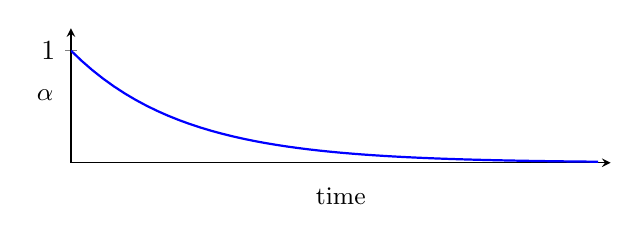
\begin{tikzpicture}
		\begin{axis}[
		%scale=0.6,
		ymax=1.2, ymin=0, xmin=0, xmax=3,samples=50, 
		ytick={1},
		axis lines=left, 
		xtick=\empty,
		yscale=0.3,
		ylabel style={rotate=-90},
		ylabel={\small $\alpha$},
		xlabel={\small time},
		%		every axis x label/.style={
		%			at={(ticklabel* cs:-0.5)},
		%			anchor=south,
		%		}
		every axis x label/.style={at={(current axis.south)},below=2mm},
		every axis y label/.style={at={(current axis.west)},left=1mm},
		]
		\addplot[blue, thick,domain=0:2.93] (x, 5^-x);
		%\addplot[red,  ultra thick] (x*x,x);
		\end{axis}
		\end{tikzpicture}
		\caption{Desired impact profile on $\alpha$ as a function of time}
		\label{fig:alphaTime}
	\end{center}
\end{figure}

%\subsubsection{Favoring }

\subsubsubsection{Penalizing velocity}

To also take velocity into account, we will consider the spatial length of the current movement vector $\b{\delta}$. First, we will want to ensure a responsive interface by fully discarding the past for very fast movements, i.e. some velocity threshold, but obviously not so low so as to be triggered by the inherent velocity of the noise. Also, we would like some sharp, but smooth transition in reaching this threshold, with profile as shown in figure \ref{fig:alphaVelocity}. We may capture such profile and threshold by a combined positive polynomial and cut-off function
$$\nu_n = \max \(0, 1- \lambda \norm{\b{\delta}}^2 \) $$ 
for some constant $\lambda$ determined by visual inspection.
\begin{figure}[!ht]
	\begin{center}
		\begin{tikzpicture}
		\begin{axis}[ymax=1.2, ymin=0, xmin=0, xmax=3,samples=50, 
		ytick={1},
		axis lines=left, 
		xtick=\empty,
		yscale=0.3,
		ylabel={\small $\alpha$},
		xlabel={\small velocity},
		ylabel style={rotate=-90},
		every axis x label/.style={at={(current axis.south)},below=2mm},
		every axis y label/.style={at={(current axis.west)},left=1mm},
		]
		\addplot[blue, thick] (x, 1 - 0.2 * x*x);
		\addplot[blue, ultra thick, ,domain=2.23:2.93] (x, 0);
		%\addplot[red,  ultra thick] (x*x,x);
		\end{axis}
		\end{tikzpicture}
		\caption{Desired impact profile on $\alpha$ as a function of velocity}
		\label{fig:alphaVelocity}
	\end{center}
\end{figure}

\subsubsubsection{Combined penalizations}

Incorporating the two penalizations in (\ref{eq:alphamSoothing}) gives the recurrence
\begin{eq}
%	\gamma_n
	\b{\tau_{n+1}} & = 
	\b{t_n} - \alpha_n \b{\delta}
	\\ & =
	\b{t_n} -   \pi_n \nu_n   \b{\delta}	 
	\\ & =
	\b{t_n} - \( \gamma^{-t} \) \( \max(0, 1- \lambda  \norm{\b{\delta}}^2) \) (\b{t_n} - \b{\tau_n})% \b{\delta} 
\end{eq}
which is the algorithm for ensuring a smooth transition  from on-screen to off-screen space, such that the user's sense of continuity is maximized.

To conclude, we will remark briefly on the expected behavior of this. First, the penalty imposed by time is assumed to be close to constant, since the frame rate of the tracker is approximately constant. Second, rapid navigations that exceed the velocity cut-off are assumed to be rare and constitute only a minor portion of all navigation. Hence, the general swiping speeds are not expected to fluctuate wildly, but rather increase or decrease in a relatively smooth manner. As such, the penalty imposed by velocity is also somewhat constant. This means that the weights do not fluctuate much within brief time periods, such that
$$\alpha_0 \approx \alpha_1 \approx \dots \approx \alpha_n $$
. If so, the recurrence will then resemble 
\begin{eq}
	\b{\tau_{n+1}} = \ &  (1 - \alpha) \b{t_n} + 
	\\
	&  \alpha (1 -\alpha) \b{t_{n-1}} + \dots +
	\\ 
	&  \alpha^{j}   (1 - \alpha ) \b{t_{n-j}} +  \dots +  
	\\
	&  \alpha^{n+1}  \b{\tau_0}   
\end{eq}
which is the \ti{exponential average} of past observations. This is the weighting between the present and past that is assumed intuitive  for stabilizing the input in general, but one that still ensures responsiveness by favoring the present for large velocities. 



%In addition, proper callibration was straightforward to confirm by visual inspecting, i.e. that the user moving the indedx finger freely in offscreen space was reflected in accurate and responsive projection onto the offscreen (visible as a cursor) .






\twocolumn[
	\section{Implementation}\label{ch:implementation}
	]
\noi In this section we touch very briefly on design choices  and  lessons learned  from implementing and configuring the solution.\\

\subsection{Choice of runtime}

The solution was implemented in the WinRT runtime, which runs natively on the Surface Pro. It has excellent support for developing touch-enabled user interfaces, such as those found on mobile devices. It is also a newer runtime partially derived from the widely popular .NET, but with limited and complicated backwards compatibility due to being a super-subset of this.

\subsection{Mathematical routines}

Some parts of the solution rely on substantial use of linear algebra for matrix operations, decompositions etc. Stable libraries already exist for this type of logic and one popular choice, the Accord.NET framework was chosen to work with. However, this entire framework needs to be re-targeted and recompiled (to Windows 8) in order for it to work in the WinRT runtime. In addition, some parts of the source code had to be manually changed, although we will omit further technical detail here.

%\fn{On an additional and more technical note, parts of the source relating to the Enum data type needs to be removed, for elaborate reasons we omit here.}.

%\subsection{Optimizxations}
%
%necessary to convert controls to bitmap

\subsection{Application design}

The overall design of the application provides several functionalities, primarily for the calibration of spaces, execution of experiments, and data processing/extraction. Several interfaces also provide the ability for confirming application parameters  by inspection, such as projection information (lengths, delta movements etc.) and three-dimensional rendering of the tracking data as well as visual projection pointers for determining the optimal tracker setup. Part of this is shown in figure \ref{fig:meandstickman}.

\subsection{Application parameters}

As previously accounted for, some smoothing parameters needed to be determined by visual inspection. The effects of these were estimated by observing the translated off-screen interaction in the on-screen space, i.e. the projections of tracked joints of interest onto an imaginary extension of the plane spanned by the device. That its, off-screen input was visualized on-screen through the positioning of circle "cursors" in the user interface, which visually reveals any presence of noise.  

For the general smoothing that incorporates the past, an optimal $\gamma=1.0035$ was found by parameter sweeping through a value range until no jitter was visible. To reason briefly, for a frame rate of approximately 30 frames per second, this corresponds to $\pi = 1.0035^{-30} \approx 0.0573$, which is equivalent to incorporating only $1/17$ of the previous frame. As such, eliminating jitter noise compromises little on the information of the most recent tracking frame. 

As for the mechanism that ensures responsiveness, a value of $\lambda=770$ was identified as optimal in similar sweeping approach. Hence, for this choice to disregard the past completely ($\alpha = 0$), we would need to see delta movement 
\begin{eq}
	0 = \nu &= \max \(0, 1- \lambda \norm{\b{\delta}}^2 \)   \\ & \uda \\ 
	0  & \le	 1 - (770)(\norm{\b{\delta}}^2) 
	\\ & \uda \\
	\norm{\b{\delta}} & \ge 1/\sqrt{770}
	\\
	& \approx 0.0036 m
\end{eq}
, i.e. Euclidean distance of at least 3.6 millimeters for every 30 milliseconds (the aforementioned frame rate). In more comprehensible scale, this corresponds to approximately 12 centimeters per second, a number that appears reasonable as being on the border between precision and non-precision movements.



%and projection data for input interfaces (e.g. projection lengths, positions, movements etc.).

\begin{figure}[!hb]
	\centering
	\includegraphics[width=0.7\linewidth]{image/meandstickman}
	\caption{Shaking hands with oneself: visual rendering of the tracking data allows for exploring the stability and possible configurations of various tracker positionings. A sidebar (green on right) allows for adjusting smoothing parameters ($\gamma$ and $\lambda$) and a visual cursor (partly obscured red circle in center) allows for evaluating the resulting projection behavior.}
	\label{fig:meandstickman}
\end{figure}



%\begingroup
%\let\clearpage\relax

\twocolumn[
	\section{Results and Evaluation}\label{ch:evaluation}
	]

%Kinect was smoothed with values..

\noi To understand how well the \AirSwipe\ solution performs, a series of experiments were conducted, with the overall goal of providing quantifiable measurements for evaluation. Our definition of success will be the overall extent to which the solution optimizes the user experience. This will primarily be interpreted as a reduction of interaction time, but secondary factors, such as redundancy of input and sense of control, will also be taken into account.\\


\subsection{Experimental setup}

All the experiments were based on using the Surface as input device and with the smaller on-screen space artificially simulated by using rims. All tracking was done using the Kinect, which was placed in optimal conditions that were determined by experimenting with a wide variety of light conditions and tracker positions. Of all tested setups, one proved ideal in terms of providing consistently stable tracking of the body joints of interest (finger, hand and shoulder).

\subsubsection{Positioning}

The optimal positioning was found to be with the tracker having a profile view of the device and in equal height to it. Relative to the user, the tracker was placed on the side opposite to the interacting hand. As the user was distanced an arms-length (approx. $0.5$ meter) from the device, this left the tracker with an angled forward view of the individual to track (as is required by its design). This setup, depicted in figures \ref{fig:experimentalSetupProfile} and \ref{fig:experimentalSetupAbove}, provided stable tracking for the full range of motion, until the user's arm reached an angle that aligned it with the body profile  (an extreme and awkward input position considered beyond the requirements of the experiment)\fn{For the curious reader, a video\cite{SolutionVideo} of an early prototype that demonstrates this experimental setup is also available.}. 

%beyond what was needed for the . This primarily applied to the side opposite of the tracker and to a minor extent to the opposite side. While this threshold did not represent a physically impossible input space, the extremity of the angle was awkward (and hence, realistic as user input possible also so).



\begin{figure}[!h]
	\begin{center}
		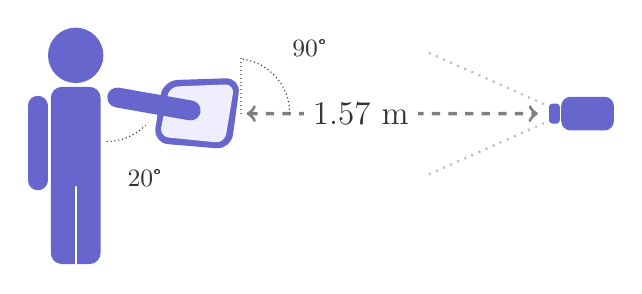
\begin{tikzpicture}%[remember picture,overlay]
		
%		{\includegraphics[]{image/stickman_front}};

		

		\begin{scope}[shift={(-4,3.9)}, scale=0.4]
	
%			\coordinate (P1) at (0,0);
%			\coordinate (P2) at (2.4,-0.2);
%			\coordinate (P3) at (2.7, 1.5);
%			\coordinate (P4) at (0.3,1.92);
			\coordinate (P1) at (0,0);
			\coordinate (P2) at (2.4,-0.2);
			\coordinate (P3) at (2.7, 2);
			\coordinate (P4) at (0.3,1.92);

			\coordinate (DEVICE_HOOK) at ($0.5*(P3)+0.5*(P2)$);
			
			\coordinate (TRACKER_HOOK) at ($(DEVICE_HOOK) + (10,0)$);

			\begin{scope}%[opacity=0.5]
			
				
		%	
	%s			\node (1) [draw, rounded rectangle]  at (TRACKER_HOOK) {rounded rectangle};
	%			\node (1) [draw, rounded rectangle]  at (TRACKER_HOOK) {rounded rectangle};
	%			
	%			\draw[thick, rounded corners=5pt,fill=black] (P1) -- (P2) -- (P3) -- (P4) -- cycle;		
				\draw[thick, rounded corners=5pt,fill=\themeColorDark,\themeColorDark] (P1) -- (P2) -- (P3) -- (P4) -- cycle;
	
				\def\deviceRim{0.2}
				\drawWithBuildOption{thick, rounded corners=3pt,fill=\themeColorLight!50,\themeColorLight!50}{top color=\themeColorLight} ($(P1) + (\deviceRim,\deviceRim)$) -- ($(P2) + (-\deviceRim,\deviceRim)$) -- ($(P3) + (-\deviceRim,-\deviceRim)$) -- ($(P4) + (\deviceRim,-\deviceRim) $) -- cycle;
	
			\end{scope}

	

			\coordinate (TRACKER_WEST) at ($(TRACKER_HOOK) + (0,0)$);
			\def\trackerSize{1}
			\def\trackerRatio{2}
			\coordinate (TRACKER_NW) at ($(TRACKER_WEST) + (0,0.5*\trackerSize)$);
			
			 
%			\draw[thick, rounded corners=3pt,fill=\themeColorDark,\themeColorDark] 
%				(TRACKER_NW) -- 
%				($(TRACKER_NW) + (\trackerSize*\trackerRatio, 0)$) -- 
%				($(TRACKER_NW) + (\trackerSize*\trackerRatio,-\trackerSize)$) -- 
%				($(TRACKER_NW) + (0,-\trackerSize) $) -- cycle;
%
			\draw[<->,dashed,very thick,gray,shorten <=.15cm,shorten >=.15cm] (DEVICE_HOOK) -- (TRACKER_HOOK);

			\coordinate (SHINE_TOP) at ($(TRACKER_HOOK) + (-4,2)$);
			
			\draw[-,dotted,thick, color=gray!50,shorten <=0.1cm, ] ($(TRACKER_HOOK) + (0.5,0)$) -- (SHINE_TOP);
			\draw[-,dotted,thick, color=gray!50,shorten <=0.1cm, ] ($(TRACKER_HOOK) + (0.5,0)$) -- ($(SHINE_TOP) + (0,-4)$) ;

			
			 \draw[rounded corners=1pt, fill=\themeColorDark,\themeColorDark] ($(TRACKER_NW) + (0,-.2) $) rectangle ($(TRACKER_NW) +(0.3,-.8)$);
			 \draw[thick, rounded corners=3pt,fill=\themeColorDark,\themeColorDark] ($(TRACKER_NW) + (.4,0)$) rectangle ($(TRACKER_NW) +(2,-1)$);

			\node[align=left, fill=white,text=black!80] at ($0.5*(DEVICE_HOOK) + 0.5*(TRACKER_HOOK) - (1,0)$) {\large  1.57 m};

%			\pic [densely dotted, draw, black!80, -,"$\theta$", angle eccentricity=1.16,angle radius=1.3cm] {angle = SHINE_TOP--TRACKER_HOOK--DEVICE_HOOK};

			
			\pic [densely dotted, draw, black!80, -,"\small $90 \degree$", angle eccentricity=1.8,angle radius=0.7cm] {angle = TRACKER_HOOK--DEVICE_HOOK--P3};


%			\coordinate (SKOD) at ($(DEVICE_HOOK) - (10,0)$);
				
			 \draw[densely dotted, gray] ($(DEVICE_HOOK) + (0.2,0)$) -- ($(DEVICE_HOOK) + (0.2,0) + (0,1.8)$);
			
		\end{scope}

%%%%%%%%%%% stickman
\def\stickmanScale{4}		
%		\def\stickmanColor{black!70!white}		
\def\stickmanColor{\themeColorDark}		
\begin{scope}[shift={(-5,5)}]%, scale=\stickmanScale]

\node[\stickmanColor,circle,fill,minimum size=5*\stickmanScale] (head) {};

\node[\stickmanColor,rounded corners=\stickmanScale,minimum height=16*\stickmanScale,minimum width=4.5*\stickmanScale,fill,below = 1pt of head] (body) {};


\draw[\stickmanColor,line width=1.8*\stickmanScale,round cap-round cap] ([shift={(0.02*\stickmanScale,-0.03*\stickmanScale)}]body.north east) --++(-10:0.3*\stickmanScale);

%righ arm
\draw[\stickmanColor,line width=1.8*\stickmanScale,round cap-round cap] ([shift={(-0.04*\stickmanScale,-0.03*\stickmanScale)}]body.north west)--++(-90:0.3*\stickmanScale);


\draw[\stickmanColor,thick,white,-round cap, minimum width=\stickmanScale] (body.south) --++(90:.25*\stickmanScale);

\coordinate (A) at ($(body.north east) + (0.07, 0)$);
\coordinate (B) at ($(A) + (1,-1)$);
\coordinate (C) at ($(A) + (0,-1)$);

\pic [densely dotted, draw, black!80, -,"\small $20\degree$", angle eccentricity=1.8,angle radius=0.7cm] {angle = C--A--B};

\end{scope}
		
		

		\end{tikzpicture}
		\caption{The experimental setup, as seen from a  profile-view. This shows the participant rotated towards the viewer, for the purpose of the illustration (the actual experiment has the user standing relaxed in front of the display).}
		\label{fig:experimentalSetupProfile}
	\end{center}
\end{figure}

%%%%%%%%%%%%%%%%%%%%%%%%%%%%%%%%%%%%%%%%%%%%%%%%%%%%%%%%%%%%%%%%%


\begin{figure}[!h]
	\begin{center}
		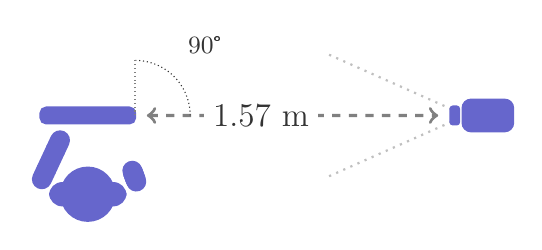
\begin{tikzpicture}%[remember picture,overlay]
		
		%		{\includegraphics[]{image/stickman_front}};
		
		\begin{scope}[shift={(-4.9,3.9)}, scale=0.4]
		
		\coordinate (P1) at (0,0);
		\coordinate (P2) at (3,0);
		\coordinate (P3) at (3, 0.5);
		\coordinate (P4) at (0,0.5);
		
		
		\coordinate (DEVICE_HOOK) at ($0.5*(P3)+0.5*(P2)$);
		
		\coordinate (TRACKER_HOOK) at ($(DEVICE_HOOK) + (10,0)$);

%		\draw[thick, rounded corners=4pt, fill=transparent] (P1) -- (P2) -- (P3) -- (P4) -- cycle;		
		\draw[thick, rounded corners=2pt,\themeColorDark,fill=\themeColorDark] (P1) -- (P2) -- (P3) -- (P4) -- cycle;
	
		
		\coordinate (TRACKER_WEST) at ($(TRACKER_HOOK) + (0,0)$);
		\def\trackerSize{1}
		\def\trackerRatio{2}
		\coordinate (TRACKER_NW) at ($(TRACKER_WEST) + (0,0.5*\trackerSize)$);
		
		
		%			\draw[thick, rounded corners=3pt,fill=\themeColorDark,\themeColorDark] 
		%				(TRACKER_NW) -- 
		%				($(TRACKER_NW) + (\trackerSize*\trackerRatio, 0)$) -- 
		%				($(TRACKER_NW) + (\trackerSize*\trackerRatio,-\trackerSize)$) -- 
		%				($(TRACKER_NW) + (0,-\trackerSize) $) -- cycle;
		%
		\draw[<->,dashed,very thick,gray,shorten <=.15cm,shorten >=.15cm] (DEVICE_HOOK) -- (TRACKER_HOOK);
		
		\coordinate (SHINE_TOP) at ($(TRACKER_HOOK) + (-4,2)$);
		
		\draw[-,dotted,thick, color=gray!50,shorten <=0.1cm, ] ($(TRACKER_HOOK) + (0.5,0)$) -- (SHINE_TOP);
		\draw[-,dotted,thick, color=gray!50,shorten <=0.1cm, ] ($(TRACKER_HOOK) + (0.5,0)$) -- ($(SHINE_TOP) + (0,-4)$) ;
		
		
		\draw[rounded corners=1pt, fill=\themeColorDark,\themeColorDark] ($(TRACKER_NW) + (0,-.2) $) rectangle ($(TRACKER_NW) +(0.3,-.8)$);
		\draw[thick, rounded corners=3pt,fill=\themeColorDark,\themeColorDark] ($(TRACKER_NW) + (.4,0)$) rectangle ($(TRACKER_NW) +(2,-1)$);
		
		\node[align=left, fill=white,text=black!80] at ($0.5*(DEVICE_HOOK) + 0.5*(TRACKER_HOOK) - (1,0)$) {\large  1.57 m};
		
		%			\pic [densely dotted, draw, black!80, -,"$\theta$", angle eccentricity=1.16,angle radius=1.3cm] {angle = SHINE_TOP--TRACKER_HOOK--DEVICE_HOOK};
		
		
		\pic [densely dotted, draw, black!80, -,"\small $90 \degree$", angle eccentricity=1.8,angle radius=0.7cm] {angle = TRACKER_HOOK--DEVICE_HOOK--P3};
		
		\draw[densely dotted, gray] (DEVICE_HOOK) -- ($(DEVICE_HOOK) + (0,1.8)$);
		
		\end{scope}
		
		
		
		\def\stickmanScale{4}		
		%		\def\stickmanColor{black!70!white}		
		\def\stickmanColor{\themeColorDark}		
		\begin{scope}[shift={(-4.3,3)}]%, scale=\stickmanScale]
		
			\node[\stickmanColor,circle,fill,minimum size=5*\stickmanScale] (head) {};
			
%			%body
			\node[\stickmanColor,rounded corners=1.2*\stickmanScale,minimum height=2.2*\stickmanScale,minimum width=7*\stickmanScale,fill,] (body) {};
			
			
			%righ arm
			\draw[\stickmanColor,line width=1.8*\stickmanScale,round cap-round cap] ([shift={(0.04*\stickmanScale,-0.03*\stickmanScale)}]body.north east) --++(110:0.1*\stickmanScale);
			
			\draw[\stickmanColor,line width=1.8*\stickmanScale,round cap-round cap] ([shift={(0.05*\stickmanScale,0.2*\stickmanScale)}]body.west)--++(-115:0.2*\stickmanScale);
			
%			\draw[\stickmanColor,line width=1.8*\stickmanScale,round cap-round cap] ([shift={(-0.04*\stickmanScale,0.08*\stickmanScale)}]body.west)--++(-90:0.1*\stickmanScale);
			
	%		\draw[\stickmanColor,thick,white,-round cap, minimum width=\stickmanScale] (body.south) --++(90:.25*\stickmanScale);
		
		\end{scope}
		\end{tikzpicture}
		\caption{The experimental setup, as seen from above.}
		\label{fig:experimentalSetupAbove}
	\end{center}
\end{figure}


\subsubsection{Lighting}

It was found that high volumes of both artificial and natural light had a negative impact on the tracking, which correlates with the general Kinect guideline of lower lighting conditions. Hence, only a minor degree of (non-direct) daylight was allowed into the test room and only in direction with the tracking device's point of view.


\subsubsection{Simulated On-screen Dimensions}

As the Surface has a significantly larger display than that of current small mobile device, a strategy for simulating the latter was necessary. Swiping outside the boundaries of a small mobile display will usually move outside the dimensions of the actual device, since the two are essentially equal. Hence, going into off-screen space will be marked by a loss of modality (touch) and introducing similar feedback will  therefore approximate real-world conditions better.

\begin{figure}[!b]
	\centering
	\includegraphics[width=0.5\linewidth]{image/chopsticks}
	\caption{The frame used for simulating a small input space, chosen to align with the display dimensions of a popular and small mobile device, the Samsung S6. Here shown overlaid with its close relative, the Samsung S4.}
	\label{fig:chopsticks}
\end{figure}

\begin{figure}
	\centering
    \includegraphics[width=0.5\linewidth]{image/rims}
	\caption{The simulating of the dimensions of a smaller mobile device, achieved by fixating a low-profile frame onto the display.}
	\label{fig:rims}
\end{figure}



The chosen approach was therefore to employ physical rims to define the smaller input space. These have some height, such that the user is given noticeable feedback in transitioning outside the boundaries. Also, this height catalyzes the off-screen interaction by "forcing" the finger into mid-air. In detail, a rectangular frame  was carefully constructed, such that it had height 4mm the and the exact inner dimensions of $4.436 \text{mm} \times 2.495  \text{mm}$, which is representative of one currently popularized smaller mobile device. This is  shown  in figure \ref{fig:chopsticks}. The frame was then fixated onto the Surface, in such a way that it aligned perfectly with the form factor of the device. The device was then  ready for calibration with the implementation. This construction and its calibration is shown in figure \ref{fig:rims}. 




















	\subsection{Experiment one: spatial definitions}

Initially, it was sought to explore through experimentation how different definitions of off-screen space  compared against each other, including a baseline derived from using on-screen space (touch) only. The three different off-screen space definitions were chosen to test separately, as previously accounted for. For each of these, different dimensionalities were explored in isolation through variations of an appropriately designed number-panning task. 

\subsubsection{Tasks}

The participants were asked to perform a panning task, conceived so as to be easily comprehensible and yet capable of efficiently capturing the desired metrics. Each exercise presented the participant with the simple concept of dragging a line with numbered tick marks in some numerical range that exceeded the on-screen viewport by several factors. The size of the input space was then equal to the length of this range (as visualized by the line), with an added $\ifrac{3}{4}$ of the on-screen viewport as "buffer" on each side. This buffer was added to ensure that navigating to an extreme of the input space still left $\ifrac{1}{4}$ of the line in view, thereby avoiding any loss of spatial orientation. 

Each value on the line was made clearly visible as a contrast overlay on the corresponding tick mark. The  task was then to drag the line until a particular trial "target value" came into center-view  of a bullseye-circle (of 3.0 centimeters in diameter). This circle, initially red, turns green when the target value is positioned within its enclosing space. In order successfully complete the trial, the participant was then required to continuously hold the value within that space for 3 seconds. Each trial was fully recorded with e.g. various vector data, such as target and release positions, and durations from initial interaction until completion of the exercise.

Ideally, the task would be designed to cover a full systematic exploration in two dimensions. But due to the extent of such an experiment, this would likely fatigue the participants and decrease the quality of the data to collect. Hence, only two dimensionalities, horizontal and vertical, were included and examined in isolation. Two variations of the task were therefore designed:

\begin{itemize}
	\item \tb{Exercise \ti{a}} aligns the line of numbers with the  horizontal dimension and places the positive range of values on the right-hand side of the origo (under the assumption  that a left-to-right increasing order is culturally appropriate for the test subject)\\
	\item \tb{Exercise \ti{b}} is as the previous, except the line is angled vertically and lists the positive numbers on the upper half (assuming the intuition of height is appropriate choice for the test subject)   
	%	\item \tb{Exercise three} combines the two dimensions and angles the line differently for each trial,  although with the positive range always in the upper-half, under the same assumptions as that of exercise two.
\end{itemize}


\begin{figure}
	\centering
	\includegraphics[width=0.8\linewidth]{image/e1exercise}
	\caption{The initial viewport of the input space in exercise \ti{a} (left) and \ti{b} (right, as used in experiment one.}
	\label{fig:expOneExecises}
\end{figure}


%\begin{figure}
%	\centering
%%	\subfigure[Title A]{
%	\includegraphics[width=0.7\linewidth]{image/expTwoDimsNeg}
%	\caption{An instance of The experimental exercise with negative target value. }
%	\label{fig:expTwoDimsNeg}
%\end{figure}




%Hence, the initial values visible to the user are in the range of TODO for the horizontal layout, TODO for the vertical and [TODO to TODO] for the two-dimensional layout, depending on the angling of the line (which is maximized on the diagonal of the input space). 

The two exercises, shown in figure \ref{fig:expOneExecises}, share equal tick-mark distances and have approximately the same initial visible input range, $[-3..3]$ for task \ti{a} and  $[-2..2]$ for task \ti{b}, which is assumed to provide an adequate sense of spatial scale. They share the same numerical tick range of $[-50..50]$ and therefore have equal dimensions of input space, which spans a  distance of 1 meter. This choice of physical range is estimated to be somewhat beyond the comfortable motion range for the average user, and as such, the experiment is assumed to cover (and go slightly beyond) fringe conditions.

As previously work has shown, loss of spatial awareness is an issue on small mobile devices unless countered and may therefore also be an issue for the experimental design used here. For instance, high navigation velocities will likely be disorienting, since the only spatial references are the line numbers, which can only be read at idle or slow speeds. In addition, the user should obviously not be left without any visual references at all, as this would lead to a total loss of orientation.
% any navigation that positions the viewport with the line out of view then leaves the user with no visual references at all.

These considerations were found to be very relevant, given the extreme simplicity of the task design. That is, the simplicity of the design is considered more detrimental to spatial awareness than most normal user interfaces. This was sought countered by minor design decisions. 

First, it was assumed that any user interface interaction starts out with some clear reference of location. For instance, opening a text document usually starts out on the first page. Likewise, digital maps usually start out in a location familiar to the user. To align with such observations, it was  assumed desirable to have the user consistently start in a well-known location, regardless of the particular trial parameters. The start location was therefore chosen to always be the origo (center) of the line, as opposed to e.g. some randomization. 

Second, it was assumed that for any user interface, some indications of spatial awareness will be present during both low and high navigational velocity. To exemplify, the pages of a document are distinctly different and rapidly enumerating them still provides some awareness in the form of quick glances of the unique outline of each page. This same reasoning applies to map navigation, since any top-down map view has a distinct topographical outline that is perceivable during both slow and fast location changes. Thus, to provide some awareness feedback during navigation, the tick marks were therefore made to increase in size and elliptical shape with increasing distance from the origo. Such design provides subtle hints that support spatial awareness,  regardless of the navigational velocity. 

In addition, a pilot test of the trials showed that users may mistake positive and negative target values. Both the  target value indicator and line tick marks were therefore color coded, with negative numbers in cold color and positive numbers in warm. This color-coding is shown in figure \ref{fig:expTwoDimsPosNeg} for a trial variant from one of the subsequent experiments. 

All in all, the decisions made here are assumed to bring the trial design  closer to the general user interface characteristics of smaller mobile devices. 


\begin{figure*}
	\centering
	\begin{minipage}[b]{0.484\textwidth} %.33
		\includegraphics[width=1\linewidth]{image/expTwoDimsNeg}
	\end{minipage}
	\begin{minipage}[b]{0.5\textwidth}
		\includegraphics[width=1\linewidth]{image/expTwoDimsPos}
	\end{minipage}
	\caption{Two instances of the experimental trial variant used in experiment three, with a negative target value on the left and positive on the right. Color coding of the indicated target value mitigates sign confusion, an inherent weakness in this type of experimental design.}
	\label{fig:expTwoDimsPosNeg}
\end{figure*}

\subsubsection{Input interfaces}

To provide a reference point for comparison, a baseline was first derived by completing the two tasks in an interface that allowed touch input only. Next, each off-screen space definition of interest was explored as a separate interface, again using the same two tasks, $a$ and $b$. 

%Minor visual feedback was given to provide . The background would initially be neutral (white) and yield a subtle but perceivable  
%for both the initiation of touch input and the subsequent transition into off-screen space

%, with one task per definition.


%The experimental interfaces were based on the desire for exploring all given definitions of the off-screen space, of which three have been given. In addition, isolating and evaluating all combinations of input dimensionalities were assumed to be desirable, since the solution may yield differing effects for different ones. With all three off-screen definitions being based on a planar extension of the display, these dimensionality combinations are covered by horizontal input, vertical input and both them combined. Thus, with three definitions and three dimensionality combinations, a total of nine interfaces were tested.



\subsubsubsection{Baseline}

\def\nativeInertiaFn{Using the \href{https://msdn.microsoft.com/en-us/library/windows/apps/windows.ui.xaml.uielement.manipulationmode.aspx}{ManipulationDelta} event provided by the WintRT framework.} %\fn{\nativeInertiaFn}
As mentioned, the baseline was derived with input confined to the on-screen space only and no use of off-screen space. Exclusive to the baseline is the incorporation of inertia, a navigational aid so common in touch-enabled interfaces that it was considered required in order for the baseline to generalize well. For this same reason, the implementation of inertia was done so as to align its behavior with what is presumed normal to most users. The inertia reference of choice was therefore that of a widely known map service provider\fn{Google maps}. Using  on-screen inertial delta movement vector $\b{\delta}$ and its associated velocity $v$ (both provided by the chosen framework), the modified inertia delta movement $\b{{\hat\delta}}$ that most closely resembles the desired behavior was found to be the exponentially decreasing
$$ 
\b{\hat\delta} =   2.7^{ - \(\large \ifrac{  \hat{v}} {v} \)} \b{\delta}  
$$
%where and are the incremental movement and velocity vectors of the input,  
where $\hat{v}$ is the velocity of the last non-inertial movement before the intertia was initiated. Furthermore, the magnitude of the velocity was scaled by 
$$ v = \min( v, 7.3 ) $$
to enforce an upper ceiling that avoids extreme inertia. Such a ceiling is necessary on a touch-enabled device, because excessive swipe velocities do occur frequently and applying the corresponding inertia will result in loss of spatial awareness unless capped.   


\subsubsubsection{Plane-orthogonal}

The simplest of the off-screen definitions, this interface projects the user's finger in a line orthogonal to the plane. The user may then continue the swipe off-screen, as if an imaginary virtual extension of the display was present in the plane spanned by the device.

\subsubsubsection{Plane-directional}

Here, the projection follows the direction of the participants finger, defined as the vector from the base of the index finger and to the tip\fn{In detail, some minor offset is applied through visual inspection during calibration, since the tracker provides a fix on the center of the hand (rather than the base of the index finger, as is the desired point to approximate for deriving pointing direction).}. As the extension of the display is still planar, the velocity of navigational movements then depends not only  on the orthogonal distance from the finger to the plane, but also its angle with the plane's normal.

\subsubsubsection{Spherical}

The most complex of the interfaces, this allows for interacting with off-screen space through projecting onto a sphere. This sphere is centered at the user's shoulder, with radius equal to the shoulder's orthogonal distance to the plane spanned by the device. This distance is assumed to correspond to the length of the user's arm, such that the finger ideally remains at the boundary of the sphere, regardless of the input position. Although this definition of radius is in fact dynamic (calculated for each received tracking frame), the user is presumed to not move around relative to the device and thus, the radius will be close to constant. However, should the user choose to move further from the device for whatever reason, the projections will take on a more directional behavior (i.e. a simple enlargement of the sphere), which is still presumed intuitive to most users.

% spherical approximation of the motion range of the user's arm and thereby invariant to the exact positioning of the user, given that the distance of the shoulder to the display plane remains relatively constant.

%
%\subsubsection{Horizontal}
%
%\subsubsection{Vertical}
%
%\subsubsection{Horizontal and vertical}
%
%

\subsubsection{Trial design}

To conduct the experiment for a given interface and task, participants had to complete a set of trials, each asking for navigating to a target value unique to the task. In other words, the relation between trials and target values is a bijection. 

The set of target values was conceived on three assumptions. First, the range should cover the presumed physical limit (i.e. a line length of one meter). Second, the target values should be equally spaced to provide interpretable results. Third, the steps should be numerically simple, under the assumption that humans do not relate odd-sized numbers very well to each other. 

To take these assumptions into account, the 10 symmetrical target values 
%$$\[-50,-40,-30,-20,-10,10,20,30,40,50\]$$
$$\pm\{10, 20, 30, 40, 50\}$$
%$$\{t \mid -50 \le t \le 50, t\mod 10 = 0\}$$
were chosen as the target value set for full and evenly spaced coverage of the input range, with the step size (10) presumed optimal in terms of  numerical comprehension. 

Both the interfaces and task exercises were executed in the order presented here. For each interface, all target values were systematically randomized, using a unique string identifier for each participant as seed (for reproducibility while uniquely randomizing for each participant). 
%In addition and specific to the two-dimensional exercise, is the additional choice of line angles that ideally should cover the full spectrum. Hence, for this exercise type, the trials have unique and equally spaced angles, with the combined set covering the full range of angles (i.e. one half-circle, since the positive range is to be in the upper half by design choice). As with the target values, this set of angles is randomized using the aforementioned seed.



All in all, a total of 5 participants $\times$ 4 interfaces $\times$ 2 tasks $\times$ 10 trials = 400 trials were recorded. % 5 x 4 x 2 x 10


\subsubsection{Procedure}

Participants were given an introduction and demonstration to the general procedure for completing trial instances of the two task variants for both negative and positive numbers. Next, a few practice sessions were completed so as to get comfortable with the situation. Each participant was placed in front of the on-screen input space in a position that allowed for a natural and relaxed use of the interacting arm. In addition, participants were informed that the off-screen interfaces varied slightly, but no other hints were given, in order to obtain results that accurately reflect how well a given interface performs on the premise of the \ti{user's} intuition. That is, the aim of the procedure was to prevent data pollution by ensuring that the user did not try to conform to any predefined notions of off-screen space. 

%That is, with the experimental end goal of uncovering the user's perception of input space, the aim of the procedure was to prevent data pollution by ensuring that the user did not try to conform to any predefined notions of the space. 



%qusationanare..TODO
%All american participants informed about dimension of information space : 1m approx 40 inch

\subsubsection{Participants}

Two males and three females agreed to participate in the experiment. All were in the age span 20-40 (mean 29, standard dev. 9.3), all had normal vision and all chose to interact with the right hand.

\begin{figure}[!h]
	\centering
		\includegraphics[width=1\linewidth]{image/collage}
	\caption{Happy and healthy Silicon Valley techies in their prime, all presumed quick to engage with new technology.}
	\label{fig:collage}
\end{figure}


\subsubsection{Hypothesis}

It was hypothesized that a simple extension of the plane would best align with the users' perception of off-screen space, since the display itself is planar.  Hence, the plane-normal interface was expected to yield the shortest interaction times (H1).

Adding directional capabilities, i.e. allowing the user to navigate a planar extension by anchoring  to the directional projection of the finger, was assumed difficult to manage for two reasons. For one, directional projection obviously has little effect in close proximity to the display, due to the projection distances being short. On the other hand, the velocity was expected to become too sensitive outside the display, since the convex curve formed by the motion of the arm will increase directional projection distances very rapidly (from zero and to infinity for when the arm is parallel with the plane). Hence, the plane-directional interface was expected to equal the plane-normal interface for low target values, but overshoot for the high targets due to uncontrollable velocities, possibly with additional clutches for regaining navigational control and sensitivity (H2).  

Introducing a curve in the off-screen space was presumed to maximize continuous (single-touch) travel distances while keeping the sensitivity constant. However, the transition in moving from a visible plane to an invisible curvature was assumed disorienting  and with the user likely to follow a plane rather than the depth of the sphere. This would presumably result in undershooting of degree increasing with target value, making the spherical interface slow and clutch-based for high target values (H3).

Lastly, all off-screen interfaces were expected to perform less optimally for the side of the non-dominating hand due to more constrained movement and obstruction of view, as has been shown to be the case in previous work\cite{adbin}(H4).

%\cite{adbin}
%TODO: dominating side
%
% ... expect optimal results on side of  dominating hand, as per \cite{adbin}  TODO.
% 

\subsubsection{Results}

To reduce noise, outliers were detected and removed for each type of interaction, defined as the unique combination of an  interface, dimension and target value. 

Trials were identified as outliers if their duration violated an upper fence, which we define as the full interaction time exceeding three interquartile ranges above the upper quartile (Q3) or under the lower quartile (Q1). In addition, any trial taking above a hard limit of 25 seconds were bluntly categorized as an outlier\fn{Such an instance corresponds to \ti{at least} 5 seconds for every interval of target value (0.1 meter) - clearly an extreme duration and one that has significant impact on the interquartile range, due to the smaller sample size.}. In numbers, three trials from three separate participants were removed (plane-normal, horizontal: 1, directional, horizontal: 1, spherical, horizontal: 1).



%PlaneNormal, dims mode: Horisontal: 1
%Directional, dims mode: Horisontal: 1
%Spherical, dims mode: Horisontal : 1

\subsubsubsection{Baseline}

As seen in figure \ref{fig:expOneBaselineData}, the duration for the baseline could appear to be approximately linear in the target value, or put differently, linear in the distance to cover. In numbers, we see durations of approximately four through seven seconds. There is a slight tendency for the curve to  flatten out at target extremums. A  possible explanation for this may be found on the right-hand side of the figure, where it is seen that inertia covers almost all the travel for high targets and is presumably of high velocity. 
One particular trait of the inertia  appears to be an immediate and rapid increase for positive target values, which correspond to the side of the participant's interacting hand. This is sensible, since the only way to avoid obstructing the display for an east-to-west swipe motion is to interact quickly (by removing the hand and letting inertia do the traveling). %This would also be supportive of existing research. 

Overshoot statistics is also shown by the figure, defined as the accumulated travel distance taking place after the target has entered and prematurely exited the bulls eye, over the total travel distance. As is seen, overshooting could appear to decrease slightly with increasing target values. This is somewhat counter-intuitive, as one may expect greater inertia velocities at higher target values and therefore more overshooting. However, the noticeable spike for the horizontal dimension and target 20 could possibly indicate that users tend to apply inertia in a very rough and invariant manner regardless of the target, which would consistently result in more overshooting for smaller (nearby) targets.

The statistic on the number of touches (which are shown in absolute values  rather than percentage) indicate that user's perform a touch for every 0.1 meter. Thus, targets highs such as 50 require approximately five touch operations, which implies significant redundancy in the physical input for the baseline. 

%
%Also, the intertia travel ratio as seen in figure TODO.
%
%Also, the touch count as seen in figure TODO.


%\def\expOneProjectionMode{Horisontal} 


\begin{figure*}[!ht]
	\centering
%	\vspace*{-1cm}
	%	\def\plotHideYLabel{ylabel={\textcolor{white}{}}, yticklabels={,,}}
	\begin{tikzpicture}
	\threeFigureTrialMode{Baseline}{\meanColor}
	{ymax=25, y post scale=1}
	{ymax=85,y post scale=1, legend style={at={(axis cs:0,\plotYMax*.95)}} }
	\end{tikzpicture}		
	\caption{The baseline data collected for the horizontal dimension (top) and vertical (middle). The two combined is also shown (bottom), in order to obtain an idea of how a true two-dimensional interface is likely to perform. The left-hand side of each row shows the duration data in lightly scattered form, along with the mean (that does not include outliers). On the right-side of each row, statistics is shown for the mean percentages of overshoot and inertia travel, as well as the mean number of touches used (note the latter is in absolute values and is amplified by a factor of 10, to distinguish it more clearly on the scale used).}
	\label{fig:expOneBaselineData}
\end{figure*}



\subsubsubsection{Plane-normal}

In figure \ref{fig:expOnePlaneNormalData}, wee see that the duration for the plane-normal bears strong resemblance with the baseline, although slightly more fluctuating and with an overall pattern of longer durations. Interaction now takes upwards of 12 seconds in general. Overshooting appears more arbitrary and difficult to interpret. The number of touches and redundant input  is significantly lower however and only rises above a single one (the initiating touch) for target values of 40 or greater. 

\begin{figure*}[!ht]
	\centering
	\vspace*{-2cm}
		%	\def\plotHideYLabel{ylabel={\textcolor{white}{}}, yticklabels={,,}}
	\begin{tikzpicture}
	\threeFigureTrialMode
		{PlaneNormal}
		{\meanColor}
		{ymax=25, y post scale=1}
		{ymax=85,y post scale=1}  %legend style={at={(axis cs:0,\plotYMax*0.98)}}
	\end{tikzpicture}		
	\caption{The data collected for the plane-normal interface. Inertia data do not exist here, as it is not a feature of any of the off-screen interfaces.}
	\label{fig:expOnePlaneNormalData}
\end{figure*}

%	\caption{}
%	\label{fig:}


\subsubsubsection{Plane-directional}
%

The plane-directional interface results in the data shown in figure \ref{fig:expOneDirectionalData}. Again, durations are significantly more fluctuant and take upwards of 11 seconds, slightly worse than the baseline. What stands out for this interface though, is the close-to elimination of subsequent touch operations. Conversely, there is significant overshooting for all intermediary values. While speculative, the drop in overshooting at the extremes may possibly be a result of the user performing a release before reaching the target value hold. This would be supported by the concurrent rise in touch count for high target values and could indicate difficulty in controlling the interface at high targets. Not shown by the plots, but noted by two of the participants, is that the directional projections became more "jittery" at high target values, which again supports this theory.

%\onecolumn
%\newpage
%\pagebreak
%\twocolumn


\begin{figure*}[!ht]
	\centering
	%	\def\plotHideYLabel{ylabel={\textcolor{white}{}}, yticklabels={,,}}
	\vspace*{-2cm}
	\begin{tikzpicture}
	\threeFigureTrialMode{Directional}{\meanColor}{ymax=25, y post scale=1}{ymax=85,y post scale=1}
	\end{tikzpicture}		
	\caption{The data for the plane-directional interface.}
	\label{fig:expOneDirectionalData}
\end{figure*}

\subsubsubsection{Spherical}

The data of the last remaining interface is illustrated in figure \ref{fig:expOneSphericalData}. This could appear to have the lowest variance of all three off-screen definitions. Also, the interaction durations are slightly better than the all past off-screen interfaces and come very close to the baseline, with an approximate maximum of nine seconds for  extreme targets . Overshooting is almost non-existing and the same applies to subsequent touch operations, there are almost none.

\begin{figure*}[!ht]
	\centering
	\vspace*{-2cm}
	%	\def\plotHideYLabel{ylabel={\textcolor{white}{}}, yticklabels={,,}}
	\begin{tikzpicture}
	\threeFigureTrialMode{Spherical}{\meanColor}{ymax=25, y post scale=1}{ymax=85,y post scale=1}
	\end{tikzpicture}		
	\caption{The data for the spherical interface.}
	\label{fig:expOneSphericalData}
\end{figure*}



\subsubsection{Discussion}

To sum up and evaluate, we will compare the general behavior of each interface, as captured by their means. Furthermore, we will view the combined dimension as the most meaningful to compare, under the assumption that future use of off-screen space is likely to be for  two-dimensional interfaces. Such comparison is given in figure \ref{fig:expOneMeansCompared}. From this, it appears that the spherical interface aligns best with the baseline and is most stable. We therefore dismiss the original idea that the plane-normal should perform optimally in terms of duration time (H1).

For the plane-directional interface, this did indeed result in significant over-shooting, increased touch counts and was inferior from a time-perspective. This supports the initial presumptions about the interface (H2), which are therefore confirmed.

Contrary to what was expected, the spherical interface did not suffer from long durations and came quite close to the baseline. In addition, this interface had virtually no touch input redundancy and almost zero overshooting. This hypothesis (H3) is therefore rejected.

As previously touched upon, a right-handed interaction may possibly obstruct part of the view for  when the user initiates an on-screen swipe that ends in the north or west. With regards to the test interface, this corresponds to seeking out high target numbers in the horizontal dimension and low target numbers in the vertical. Thus, the data for these targets should show disproportionately longer durations, if the assumption of negative impact is true. However, the data does not indicate any significant pattern that strongly supports this view. This leaves the general assumption (H4) rejected for now and any minor effects to be explored more intricately in future work.

On a final note, it is assumed that the baseline has been significantly advantaged in this experiment, since the participants are all experienced with that interface and conversely, are all new to the idea of using off-screen input. Hence,  the baseline may have appeared best in terms of duration, but the picture could likely be different, had all interfaces been on par in terms of user experience. In addition, all off-screen interfaces are presumed to greatly enhance the user experience by  eliminating redundancy in the input, as was observed here. This allowed participants to locate target values in a single motion (except for the extremums that occasionally required an additional touch operation). Whether any  incurred   strain of off-screen interaction have a negative impact, such as the physical fatigue identified in previous work\cite{peep}, is yet another topic left for future research.  




%\def\(#1\){\left(#1\right)}


\begin{figure}[!ht]
	\centering
	%	\begin{scaletikzpicturetowidth}
	\hspace{-1cm}
	\begin{tikzpicture}[]%[rotate=90]
	\begin{axis}[
%	scale=2, 
	smooth,
	xmajorgrids=true, ymajorgrids=true, 
	ymin=0, ymax=15,		
	%	domain=-50:50,
	xmin=-55,xmax=55,
	%		nodes near coords,
	xlabel={Target value},
	ylabel={Duration (seconds)},
	xtick distance={10},
	legend style={draw=none},
	legend entries={
		baseline,
		plane-normal,
		plane-directional,
		spherical},	
	legend style={
		font=\scriptsize\selectfont,
		at={(axis cs:-3,14)},anchor=north
	}
	%	legend pos=outer north east
	%	legend pos=inner north
	]
	
	%	\addlegendimage{no markers,green}
	%	\addlegendimage{no markers,blue}
	%	\addlegendimage{only marks, mark=o}
	%	\addlegendimage{only marks, mark=square}
	\addlegendimage{thick,no markers, \meanColor}
	\addlegendimage{thick,no markers,\myRed}
	\addlegendimage{thick,no markers,\myGreen}
	\addlegendimage{thick,no markers, \myBlue}
	%	444444\addlegendimage{only marks, mark=square}
	
	\drawAxes				
	
	\edef\plotX{trialTargetValue}
	\edef\plotY{trialDurationSeconds}
	\edef\plotErrorMarginColName{trialDurationSecondsConfidence}
	
	\def\trialGroupName{DimsConcatenationAveraged}
	\expOnePlotMean{Baseline-\trialGroupName}{y error=}
	\expOnePlotMean[\myRed]{PlaneNormal-\trialGroupName}{y error=}
	\expOnePlotMean[\myGreen]{Directional-\trialGroupName}{y error=}
	\expOnePlotMean[\myBlue]{Spherical-\trialGroupName}{y error=}
	
	%	\edef\trialGroupName{Baseline-TwoDimensional}
	%	\expScatterPlotMean{}
	%	\addlegendentry{Baseline}
	
	
	%	\edef\trialGroupName{PlaneNormal-TwoDimensional}
	%	\expScatterPlotMean[\myRed]{}
	%	
	%	
	%	\edef\trialGroupName{Directional-TwoDimensional}
	%	\expScatterPlotMean[\myGreen]{}
	%	
	%	\edef\trialGroupName{Spherical-TwoDimensional}
	%	\expScatterPlotMean[\myBlue]{}
	
	\end{axis}			
	
	%	\expOneScatterPlot{Baseline-TwoDimensional}{trialTargetValue}{trialDurationSeconds}{}
	\end{tikzpicture}	
	%	\end{scaletikzpicturetowidth}
	\caption{The mean for the baseline and all off-screen interface definitions. These are the combined means of the perpendicular horizontal and vertical dimensions, which are presumed to provide good insight into the interaction efficiencies of a true two-dimensional interface. }
	\label{fig:expOneMeansCompared}			
\end{figure}






	\subsection{Experiment two: learning the sphere}

Having determined the spherical interface as the most optimal, it was desired to explore this spatial definition in more detail. That is, we would like to learn how well users' expectations of the space relate to the idea of a simple sphere. Participants were therefore asked to complete a variant of the task that systematically investigates their perception of spatial targets versus their the true projections, as currently defined by the spherical interface.

\subsubsection{Tasks}

Participants were asked to perform estimations in a two-dimensional task, for combinations of target values and line angles that  correspond to dividing the entire spherical input space into a circular grid. This grid and  distribution of target  values is shown in \ref{figure:expTwoTargetLocations}. The task was then to position the input (finger) on the spatial location that corresponds to the requested target value on some line angle, as the participant perceived it.

\begin{figure}[!ht]
	%	\def\domainMax{1.2}
	\centering
	\begin{tikzpicture}[scale=0.95]	
	\expPolarAxis[			
	extra y tick labels={ 0.5m, 0, -0.5m},					
	y dir=reverse,  %%% REVERSE BECAUSE TRACKER VIEWS FROM OPPOSITE SIDE!
	%			extra y tick labels=,	
	%				hide y axis,ymajorgrids=true,yminorgrids=true,
	]{		
		\coordinate (origin) at (axis cs:0,0);			    
		
		\drawCircles
		
		\plotPolarTargetValues
		
		\begin{scope}[yscale=-1] 
		\polarPlotDrawRadials 
		\end{scope}			
		
		\drawOnscreenDims			
	}		
	\end{tikzpicture}
	\caption{The mesh of target values for experiment two, defined by the dividing of the input space into a circular grid with origo at the zero target value. As can be seen, the grid has  radials for every 30 degrees and target values for every $0.1$ meter. The rectangle at the center corresponds to the exact dimension of the on-screen input space (as derived during the calibration process). Both major grid axes align with the device form factor, such that the viewpoint corresponds to a top-down view of the plane spanned by the device.  Note the color coding convention introduced to clearly distinguish equivalent target values, a visual aid that will be used recurrently henceforth. }
	\label{figure:expTwoTargetLocations}				
\end{figure}



\subsubsection{Input interfaces}

The participants only interfaced through the spherical definition of space for estimating targets in off-screen space. However, no visual feedback of the input was given, as the very objective was to estimate locations without any attempts to conform to the interface.

 
\subsubsection{Trial design}

The variation of the experimental task was identical to that used in experiment one, except there were now two dimensions and $\ifrac{180\degree}{30\degree}=6$ differently angled input lines (each line corresponding to two opposing and aligned radials). For the angling of any line, the positive range was placed on the top-most radial and the negative range on the opposing bottom, under the assumption that this ordering was intuitive to most users. Also, all combinations of angles and target values were randomized using the same seeding technique as in experiment one.

Although no visual feedback was to be given, some indicator of trial initiation was considered meaningful. To provide this in an intuitive manner, the movement of entities was reversed, such that the bulls eye now followed the user's input, with the trial line remaining fixed instead. Hence, to initiate an estimation trial, the participant touched the screen once, after which the bulls eye began to follow the finger, quickly sliding out of view as the user's finger moved outside the boundaries of the display (to perform the estimation).

A total of 5 participants $\times$ 1 interface $\times$ 6 angles $\times$ 10 targets were estimated, yielding a total recording of 300 trials. % 5 x 1 x 1 x 60

\subsubsection{Procedure and participants}

Similarly to the previous experiment, the same set of participants were given demonstrations, practice trials and clearly advised that their intuition of target locations was the primary intention of the experiment, rather than completion time. Participants touched the on-screen space to initiate a trial, then moved to their chosen point of estimation and used a clicker to indicate completion with the non-interacting hand.

%All american participants informed about dimension of information space : 1m approx 40 inch

\subsubsection{Hypothesis}

It was hypothesized that users' assumption of space is closely tied to the spherical motion of the arm, but that actual interaction represents some departure from this ideal, due to the interplay of complex and unknown factors. That is, reality is presumed much more intricate for a variety of reasons,  such as obstruction of view and the complex interactions between the joints of the arm. %Hence, the true space was assumed to be spherical to some degree, but skewed, scaled and possible rotated around a mean not necessarily centered at the projection point of the shoulder (as has been the sphere definition so far).

\subsubsection{Results}

To obtain an initial grasp on the three-dimensional data and any potential patterns contained within it, we will seek to perform various visualizations.

\subsubsubsection{View of raw data}

Figure \ref{fig:expTwoViewPoints} shows the data color coded for each participant and from a multitude of angles. Here, it is seen that the input for all of them do in fact follow some degree of curvature around the device, both for the horizontal and vertical dimension. The data sets also differ significantly. Two of them, as indicated by violet and blue, provide vastly different takes on the input space. The first provides a close to planar input and the latter a more spherical. One of these  even goes well beyond the extremums of the scale. This has a reasonable explanation however, as the participant was observed moving a few steps from the device, in order to provide these off-scale inputs. While being an instance of unintended user behavior, it was left uninterrupted - and none of the other participants took similar "off-road" approach. 

Also seen from the top-view (bottom) of the figure, is that the input appear to be heavily skewed towards the south-west corner of the plane spanned by the device. Conversely the north-west corner is noticeably void of points. In addition, the side-view (center row) clearly reveals that participants are quick to depart out from the plane normal in the northern region, but much less so in the south. This could possibly be due to the obstruction of the body and a reluctance to pull the hand up towards the chest area, since that is an awkward and strenuous motion. These observations combined suggest a space that is not centered at the exact origo and one that does not have equivalent shapes in the northern and southern regions of the off-screen space.

%\begin{figure}[!ht]
%	\centering
%	\begin{tikzpicture}%[rotate=90]
%	\expOneScatterPlot{Spherical-TwoDimensional-Estimation}{trialTargetValue}{trialReleasePositionTargetDiff}{}{ylabel={Estimation value}, ymin=-55, ymax=55,\plotOptionRotateAroundOrigin{10}}
%	\end{tikzpicture}	
%	\caption{TEEEEESTING!!!!}
%	\label{figure:expTwoTwoDimSphericalDuration22222}			
%\end{figure}
%


%\begin{figure}[!ht]
%	\centering
%	\expScatterPlot{\expOneCsvFilepath}{
%		discard if not={trialMoveBullsEyeInsteadOfMap}{1},
%		discard if not={trialMode}{TwoDimensional},
%		discard if not={trialProjectionMode}{PlaneNormal},
%	}{}{}
%	%	\expOnePlot{data/exp1/Estimations--(\expParticipants)--PlaneNormal--TwoDimensional.csv}{}
%	\caption{ESTIMATION: TwoDimensional, PlaneNormal}
%	%	\caption{Directional, vertical,PlaneNormal.}
%	\label{figure:expOneTwoDim3}			
%\end{figure}


%%%%%%%%%%%%%%%%%%%%%%%%%%%%
%\pgfplotstableread{\expTwoPolarCsvFilepath}{\expTwoData}


%\begin{figure*}[!ht]
%	\vspace*{-1cm}
%	%	\def\domainMax{1.2}
%	\centering
%%	\begin{minipage}[t][5cm][t]{\textwidth}
%%	\end{minipage}
%%	\fullPageReleaseSpacePlots{\releaseSpacePlotAllParticipants{}{}}
%	%	\end{scaletikzpicturetowidth}
%	\caption{The total set of collected estimations with respect to the axis formed by the device and with the data  color coded for each participant. The on-screen space is shown as a red rectangle and with choice of axis as if the device is lying flat down in the origo. The z-axis then represents perpendicular distance from the device plane and the x and y axes represent horizontal and vertical dimensions respectively. To provide spatial orientation of the data patterns, three different views are shown. The top row present a perspective on the horizontal dimension (as if the viewer is kneeling down and viewing the device in profile). The  middle row inspects the vertical dimension (as if viewing the device in profile from the right-hand side). The bottom row presents a top-down view (as if the view point is straight on the device).}
%	\label{fig:expTwoViewPoints}			
%	\hspace*{-1cm}
%	\includegraphics{evaluationE2-1.pdf}
%\end{figure*}
%
%
%%\newpage
%%\begin{figure*}[!b]
%%%	\centering
%%\end{figure*} 
%
%\begin{figure*}[!t]
%%	\vspace*{-1cm}
%	\centering
%	\caption{As the previous figure \ref{fig:expTwoViewPoints}, but with color codings for each (absolute) target value.}
%	\label{fig:expTwoViewPointsByTarget}			
%	\hspace*{-1cm}
%%	\includepdf{evaluationE2-2.pdf}
%	\includegraphics{evaluationE2-2.pdf}
%\end{figure*} 
%%\ \newpage

We may also want to investigate the data color coded by target values instead, as shown by figure \ref{fig:expTwoViewPointsByTarget}. From here, it is seen that the estimations vary  little for small targets, but slowly increase and become severely scattered for the extremes. This trend of dispersion appear most pronounced in the south-east corner. Correlating this with the previous figure \ref{fig:expTwoViewPoints}, it could appear that participants struggle more or less with achieving consistent estimations in this south-east region.

\begin{figure}[!ht]	
	\centering
	\begin{tikzpicture}[scale=1.2]
			\hspace*{-0.5cm}
	\expPolarAxis[		
	extra y tick labels={ 0.5m, 0, -0.5m},					
	y dir=reverse,  %%% REVERSE BECAUSE TRACKER VIEWS FROM OPPOSITE SIDE!		
	]{	
		\drawCircles
		
		\plotReleasePositionsColorByTarget %[filter in={trialIsStatistic}{1}]			
		
%		\plotPolarTargetValues	
		
%		\expPolarPlotAngles
		
		\begin{scope}[yscale=-1] % to get the axis labels positioned correctly
		\polarPlotDrawRadials				
		\end{scope}						
		
%		\drawOnscreenDims
		%			\plotPcaRings	
		
	}	
	\end{tikzpicture}
	\caption{The estimated locations obtained from projecting each data point using the spherical interface, here color coded by absolute target value. As opposed to the top-down view of the "raw" data, height now has influence on the end location, which makes for a slightly different picture. In addition, the projection center is now the projected location of the shoulder onto the plane spanned by the device. As such, the device is not exactly in origo from this (projection) viewpoint, but should theoretically be slightly dislocated towards the north-west quadrant (since all participants are interacting with the right hand).}
	\label{fig:expTwoProjectedData}				
\end{figure}

\def\sphereProjectNote{To ensure that the reader follows, the two-dimensional view of spherical projections has an analogue in the "stretching out" of a globe onto a plane, which results in amplification of surface area. Hence, any point not in the center of the sphere will obviously have height greater than zero from the device plane and therefore show greater dislocation from this center, when compared to a top-down view of the same data in the actual space.}

\subsubsubsection{View of projected data}

To expand on the analysis, we now relate the data to their resulting projections in the spherical interface, as shown in figure \ref{fig:expTwoProjectedData}. If the spherical interface has been used in an ideal fashion, the resulting locations should show a higher degree of dispersion, compared to the "raw" top-down view, due to the added effect of height\fn{\sphereProjectNote}. What we see instead though, is somewhat equivalent density on the south-west to north-east line and  a pattern of slightly more compaction on the perpendicular north-west to south-east line. This may  indicate that the true space is compressed. To expand lightly on this,  at least one likely contributing factor would be easy to identify: the joint of the interacting arm does not have constant flex. More precisely, the arm will have some natural flex when pointing  directly at the screen, but slowly extend and eventually reach zero as the arm travels from the origo and towards the extreme target values. This effectively corresponds to a sphere of greater radius than defined by the interface, causing the user to undershoot slightly (which translates to greater compaction in the projections, as visualized here). 




%\newpage
%\pagebreak

\onecolumn

\begin{figure*}[!ht]
	\vspace*{-1cm}
	%	\def\domainMax{1.2}
	\centering
	%	\begin{minipage}[t][5cm][t]{\textwidth}
	%	\end{minipage}
	%	\fullPageReleaseSpacePlots{\releaseSpacePlotAllParticipants{}{}}
	%	\end{scaletikzpicturetowidth}
	\caption{The total set of collected estimations with respect to the axis formed by the device and with the data  color coded for each participant. The on-screen space is shown as a red rectangle and with choice of axis as if the device is lying flat down in the origo. The z-axis then represents perpendicular distance from the device plane and the x and y axes represent horizontal and vertical dimensions respectively. To provide spatial orientation of the data patterns, three different views are shown. The top row present a perspective on the horizontal dimension (as if the viewer is kneeling down and viewing the device in profile). The  middle row inspects the vertical dimension (as if viewing the device in profile from the right-hand side). The bottom row presents a top-down view (as if the view point is straight on the device).}
	\label{fig:expTwoViewPoints}			
	\hspace*{-1cm}
	\includegraphics{evaluationE2-1.pdf}
\end{figure*}


%\newpage
%\begin{figure*}[!b]
%%	\centering
%\end{figure*} 

\begin{figure*}[!ht]
	%	\vspace*{-1cm}
	\centering
	\caption{As the previous figure \ref{fig:expTwoViewPoints}, but with color codings for each (absolute) target value.}
	\label{fig:expTwoViewPointsByTarget}			
	\hspace*{-1cm}
	%	\includepdf{evaluationE2-2.pdf}
	\includegraphics{evaluationE2-2.pdf}
\end{figure*} 
%\ \newpage


\twocolumn


\vspace*{-1.3cm}

\subsubsubsection{Mean projection deviations}



\begin{figure*}[!htb]	
	\begin{centering}
		\vspace*{-1.3cm}	
		\hspace*{-1cm}			
		\twoFigure{		
			\hspace*{-1cm}
			%			\includegraphics{evaluationE2-3.pdf}			
			\begin{tikzpicture}[scale=1.2]
			%		\hspace*{-0.22cm}
			\expPolarAxis[		
			extra y tick labels={ 0.5m, 0, -0.5m},					
			y dir=reverse,  %%% REVERSE BECAUSE TRACKER VIEWS FROM OPPOSITE SIDE!		
			]{	
				\drawCircles
				
				\plotPolarTargetValues	
				
				\expPolarPlotAngles
				
				\begin{scope}[yscale=-1] % to get the axis labels positioned correctly
				\polarPlotDrawRadials				
				\end{scope}						
				
				%							\drawOnscreenDims
				%			\plotPcaRings
				
			}	
			\end{tikzpicture}
		}{
		\hspace{0.5cm}
		%			\includegraphics{evaluationE2-4.pdf}				
		\begin{tikzpicture}[scale=1.2]	
		\expPolarAxis[			
		extra y tick labels={ 0.5m, 0, -0.5m},					
		y dir=reverse,  %%% REVERSE BECAUSE TRACKER VIEWS FROM OPPOSITE SIDE!
		%			extra y tick labels=,	
		%				hide y axis,ymajorgrids=true,yminorgrids=true,
		]{		
			\drawCircles
			
			
			
			\expPolarPlotAngleAlt{0}
			\expPolarPlotAngleAlt{30}
			\expPolarPlotAngleAlt{60}
			\expPolarPlotAngleAlt{90}
			\expPolarPlotAngleAlt{120}
			\expPolarPlotAngleAlt{150}
			
			\begin{scope}[yscale=-1] 
			\polarPlotDrawRadials 
			\end{scope}			
			
			%						\drawOnscreenDims
			
			%				\draw[
			%				%	rotate=deg(\an),
			%				color=blue,very thick] (axis cs:0,0) ellipse [x radius=40.58140,y radius=32.07781,
			%%				rotate around={deg(148):(9.4,28.8)}
			%				%				rotate around={deg(148):(50,0)}
			%				];
			
			%				\draw[dashed, ->, color=brown,very thick] (origin) -- +(100,100); 			
			%				\draw[dashed, ->, color=pink,very thick] (origin) -- +(10,10); 
			
			%				\draw[color=blue,very thick] ($(origin) + (5.0, 4.7)$) ellipse [x radius=57,y radius=65,
			%				rotate around={deg(17):(5.0,4.7)}
			%				%				rotate around={deg(148):(50,0)}
			%				];
			
			
			
			
			%			\draw[
			%			%	rotate=deg(\an),
			%			color=orange,very thick] (axis cs:0,28.8) ellipse [x radius=405.8140,y radius=320.7781,
			%			rotate around={deg(148):(9.4,28.8)}
			%			%				rotate around={deg(148):(50,0)}
			%			];
			
		}		
		\end{tikzpicture}
	}
\end{centering}
\caption{The mean estimations of target values versus their "true" locations in the grid.  Each point represents the averaged estimation location for the particular angle and target value. On the left-hand side, each estimation mean is color-coded by target value and an arrow indicates the error, i.e. the magnitude and direction towards the true location. The plot on the right-hand side is identical, except color coding is by line angle instead.}
\label{fig:expTwoMeanDeviations}				
\end{figure*}


Attempting to generalize on the projection data by viewing all data points at once is overwhelming. Instead, we may derive and visualize the mean target deviations and  how much "off" they are from the corresponding grid targets. This is illustrated in figure \ref{fig:expTwoMeanDeviations}, which shows that there are indeed large differences. Notably, the participants appear to estimate too far right  of the 90 degree radial and too far left on the  opposite 270 degree radial. Such symmetry also applies somewhat to other angles as well and in a systematic way that suggests spatial compression and rotation. Also apparent, is the reluctance of participants to interact in the far north-west corner, as is implicit by the means of this region all being closely compacted and in close proximity to the origo. %One potential reason for this is that, since the sphere center is indeed anchored by the projection of the shoulder, most projection points will appear   may be that the sphere 





\begin{figure}
	\centering
	\hspace*{-1cm}							
	%	\includegraphics{evaluationE2-5.pdf}
	\begin{tikzpicture}[scale=1.1]		
	%			\hspace*{-1cm}
	\expPolarAxis{		
		\polarPlotDrawRadials
		\drawCircles		
		
		\coordinate (origin) at (axis cs:0,0);			    
		%	\def\PPM{10} % i,e. 851
		%%	\foreachTabbedCsvRowInPlot
		\pgfplotsextra{\DTLforeach*[\DTLiseq{\target}{50}]{Pca}{\xc=x, \yc=y,\xr=xr,\yr=yr,\circleAngle=deg,\target=target,\circleRadius=circleRadius,\circleRadiusM=circleRadiusM}{	
				\coordinate (circlePos) at ($(origin) + (\xc/\PPM, \yc/\PPM)$);
				% circle at origin
				\draw[color=gray!13,fill=gray!20, thick, fill opacity=0.5] (origin) ellipse [
				x radius=\circleRadius/\PPM,
				y radius=\circleRadius/\PPM
				];
			}}
			
			
			%[xshift=5pt]
			\pgfplotsinvokeforeach {0,30,60,90,120,150} {
				\expPolarPlotReleaseDiff[xshift=0pt, opacity=1]{#1}{angle#1}{trialFromTargetToReleaseVerticalLength}{north}
				%					\expPolarPlotReleaseDiff[xshift=1pt]{#1}{angle#1}{trialFromTargetToExp3ReleaseVerticalLength}{south}
			}				
			%				\expPolarPlotReleaseDiff{0}{angle0}{trialFromTargetToReleaseVerticalLength}				
			%				\expPolarPlotReleaseDiff{30}{angle30}{trialFromTargetToReleaseVerticalLength}
			%				\expPolarPlotReleaseDiff{60}{angle60}{trialFromTargetToReleaseVerticalLength}
			%				\expPolarPlotReleaseDiff{90}{angle90}{trialFromTargetToReleaseVerticalLength}
			%				\expPolarPlotReleaseDiff{120}{angle120}{trialFromTargetToReleaseVerticalLength}
			%				\expPolarPlotReleaseDiff{150}{angle150}{trialFromTargetToReleaseVerticalLength}
			
			
			
			
		}	
		\end{tikzpicture}
		\caption{A compact illustration that captures the mean deviations and corresponding confidence values (with deviation defined as Euclidean distance from estimation to target). All bars are color coded by angle, with each capturing the mean of the sum of deviations for the target at its base. Hence, these magnitudes then also capture any scatter around the true location, as opposed to the previous figure \ref{fig:expTwoMeanDeviations}.  The numeric values for mean and confidence values are given underneath each bar and in that order.}
		\label{fig:expTwoMeanBars}
	\end{figure}


To gain a better sense of the magnitude of the deviations, we will investigate using both intuition and hard numbers. Figure \ref{fig:expTwoMeanBars} provides the former in the form of a visual overview and table \ref{table:expTwoDeviationTable} the latter by the listing of numerical values. From the visual impression, the correlation between the estimation error and target values could appear linear, although  clearly not  applicable to all the data. In general however, the estimations begin to fluctuate with increasing proximity to the target range extremities, indicating that these may have been out of reach. Three of the participants gave explicit feedback in support of this view. Furthermore, the numerical data show almost a full doubling in mean deviation between the two extreme targets (-40 versus -50  and 40 versus 50). Also, the fluctuations could seem to occur for all but the compact north-east region and the trend becoming severely pronounced in opposing south-east region. Worst appears to be the latter, which shows a full 0.27 meter deviation from the extreme target (-50) on the 330 degree radial, supporting the idea of significant variance in that region. Hence, with the general pattern of overly pronounced fluctuations in the vicinity of extremums, these outer targets (40 and 50) are likely beyond the physical reach of the participants.


\begin{table}[!hb]
	\centering
%	\hspace{-4.5cm}
	\resizebox{8cm}{!}{		
		\begin{tabular}{| >{\bfseries}l | l l l l l l | >{\bfseries}l |}
	\hline 
	\scriptsize Target\textbackslash Angle & \tb{0}    & \tb{30}   & \tb{60}   & \tb{90}   & \tb{120}  & \tb{150}   & \small{Total}  \\  
	\hline 
	50                          & 0.20  & 0.15 & 0.14 & 0.20  & 0.21 & 0.16 & 1.06 \\
	40                          & 0.07 & 0.08 & 0.09 & 0.13 & 0.11 & 0.12 & 0.60  \\
	30                          & 0.11 & 0.06 & 0.10  & 0.09 & 0.07 & 0.09 & 0.52 \\
	20                          & 0.05 & 0.04 & 0.05 & 0.06 & 0.05 & 0.05 & 0.30 \\
	10                          & 0.04 & 0.02 & 0.02 & 0.04 & 0.02 & 0.03 & 0.17 \\
	-10                         & 0.02 & 0.02 & 0.03 & 0.02 & 0.03 & 0.05 & 0.17 \\
	-20                         & 0.05 & 0.06 & 0.08 & 0.11 & 0.10  & 0.07 & 0.47 \\
	-30                         & 0.07 & 0.08 & 0.06 & 0.07 & 0.06 & 0.13 & 0.47 \\
	-40                         & 0.10 & 0.10 & 0.08 & 0.11 & 0.06 & 0.13 & 0.58  \\
	-50                         & 0.18 & 0.18 & 0.17 & 0.15 & 0.11 & 0.27 & 1.06 \\ 
	\hline 
	\small{Total}                         & \tb{0.89} & \tb{0.79}  & \tb{0.82} & \tb{0.98} & \tb{0.82} & \tb{1.10}  & \tb{5.40} \\
	\hline 
\end{tabular}

	}
	\caption{The mean deviations and their various accumulations (the reader is reminded that positive targets reside in the upper/northern half of the space and negative those in the bottom/south by design).}
 	\label{table:expTwoDeviationTable}				
\end{table}


\subsubsubsection{Principal components for each target}

As has now been determined, the participants' perception of space is indeed spherical, but does not follow the input interface in the ideal manner. In more detail, there could appear to  be some compression, rotation and translation from the origo. 

%While the total sum of projected points theoretically constitute a grid-pattern rather than a Gaussian distribution around the mean, 
To approach a more concrete interpretation of the data, we will employ the heavier tool of principal component analysis. We will assume Gaussian noise for the fluctuations that occur around the absolute target values, i.e. the "rings" formed by the points for each such data set. In addition, we'll discard outliers based on  deviation from the target, i.e. the distance from the estimation and to the target location. An outlier analysis was therefore performed for each grouping of trials (with equivalent angles and target values). Extreme cases were identified,  understood as three interquartile ranges above the upper quartile (Q3) or below the lower (Q1). These outliers were not removed, but rather replaced with the mean of the non-outliers, so as to retain the weighting of the data points in the analysis\fn{ In numbers, four values were identified as outliers,  corresponding to target/angle pairs $(-50,150)$, $(-50,120)$, $(30,0)$ and $(40,120).$}.

Deriving the principal components for each target value results in the picture shown in figure \ref{fig:expTwoMeansVersusTargets}. As can be seen by the means, there is a pattern of downward dislocation that increases by target value. This indicates that the location of the mean is in fact dynamic, in that it depends on the distance from origo. As for the observed scale and rotation, the components of the smaller targets do not exhibit any significant structure. The outer does, however, and paints a clear picture of a space that is rotated 34.6 degrees, which appear to align well with the visually observed patterns of the data. %This corresponds well in terms of the general direction and rotation of the data patterns.  

%interpretation is not straight-forward, but . 




\begin{figure}[!ht]	
	\centering
				\hspace*{-1cm}			
	%		\twoFigure{		
	%			%		\hspace*{-0.22cm}
	\begin{tikzpicture}[scale=1.2]
	%		\hspace*{-0.22cm}
	\expPolarAxis[		
	extra y tick labels={ 0.5m, 0, -0.5m},					
	y dir=reverse,  %%% REVERSE BECAUSE TRACKER VIEWS FROM OPPOSITE SIDE!		
	]{	
		
		\begin{scope}[yscale=-1] 
		\polarPlotDrawRadials 
		\end{scope}			
		
		
		\plotReleasePositionsColorByTarget			
		
		%		\coordinate (origin) at (axis cs:0,0);			    
		
		\plotPcaRings
		
		\drawOnscreenDims
	}	
	\end{tikzpicture}
	\caption{The result of applying principal component analysis to five sets of point projections, formed by grouping on absolute target values. The intersects of principle components for each set is shown by the perpendicular lines (crosses) at the corresponding means.}
	\label{fig:expTwoMeansVersusTargets}				
\end{figure}



\subsubsection{Discussion}


The data collected, and the interpretations that were derived from it, did indeed indicate a space much more complex than what is captured by the simple definition of a sphere, as was the hypothesis. Hence, the spherical interface may very well be a good approximation of the true input space, but also one that does not capture essential details, such as compression, rotation, scale and translation from the origo, all properties which the data suggest exist. Furthermore, the magnitude of these effects could appear to be correlated with the projection distance from the origo. That is, the space appears circular and centered at the origo for the initial small target values and expands into increasingly elliptical form with greater dislocation from the origo as the targets increase.  This clearly makes conforming to such projection space less than straight-forward, because it then has a "third dimension" of dynamic curvature. Also, the input appeared to become fluctuant and incoherent for the  extreme target values (40 and 50), possibly indicating that these are physically out of reach. As such, the experiment has confirmed the hypothesis, but leaves any more exact definition of the true input space  open for interpretation.





	%

%\vspace*{-2cm}

\subsection{Experiment three: optimized sphere}

With experiment one having identified  the spherical interface as the superior of the three examined and experiment two   showing it as not capturing essential details, an attempt at evaluating some optimization would be desirable. The aim in this experiment was therefore to compare the spherical space against some modification derived  from it. That is, the original baseline of touch-only is not of direct interest here (as its general performance versus a spherical off-screen interface has already been shown by experiment one). A modified spherical interface was therefore derived on the basis of the data from the previous experiment two and this was experimentally  evaluated against the  non-modified version. 
 
%merits and drawbacks compared to the sphere has already been deduced in experiment one. 

\subsubsection{Task and interface}

Participants were requested to seek out target values as in experiment one, but now using a true two-dimensional task and  a target grid similar to that of experiment two (as shown in the previous figure \ref{fig:expTwoDimsPosNeg}). As learned from experiment two, the extreme target value ($\pm50$) was likely beyond physical reach and therefore omitted. The second-largest target ($\pm40$) was then considered the new fringe value. Hence, the chosen grid pattern encompasses $\ifrac{180\degree}{30\degree}=6$ lines, each with $\ifrac{40}{10}=4$ targets.


\subsubsection{Trial design}
	
All target values were randomized in fashion identical to the previous experiments.  A total of 3 participants $\times$ 2 interfaces $\times$ 6 angles $\times$ 8 targets were collected, through 288 trials in total.

\subsubsection{Procedure and participants}

% leah: 25
% mike: 22
% evan: 38
%  mean 28.33, std 8.5049

Only three of the past participants could be made available for the experiment (mean 28.3, standard dev. 8.5), although the potential data was assumed adequate for making rough interpretations. Participants were informed that the space would vary slightly between the two interfaces, but were also requested to interact based on their intuition. No learning time was given, as the task and general interface was already familiar.

%All but one of the previous participants volunteered (yeilding new mean age=TODO, std=ODO). 
	
%assuming shouldr position cannot be omitted

\subsubsection{Hypothesis}

It was assumed that the data from experiment two could be used to reach an optimization that would perform better in terms of interaction times, for all target values within physical reach. Hence, an elaborate interpretation of the past experimental data was undertaken to deduce the various properties that should be part of the optimized spherical interface.

\subsubsubsection{Choosing general properties}

The previous experiment had revealed effects such as compression, rotation and scale through the principal components of the aggregated data for  each absolute target value. The strategy chosen here was then to  modify the space by trying to conform to these, as opposed to elaborate attempts at theorizing on the complex interplay of factors that produce them (e.g. joint interactions, obstruction of view for certain inputs etc.).

To take these properties into account, it was first noted that when participants had been asked to estimate the extreme target ($\pm50$), they generally gave inputs that appeared to be at the maximum of their physical ability. Hence, the assumption was made that these estimations had in fact defined the natural boundary of the true space. That is, while being sincere attempts at providing estimations, they were just as much representative for what the participants perceived as the physical limit of extreme input. The data points for the extreme target were therefore presumed to be an indicator of a \ti{comfort zone}, for which the participants felt they were able to interact within - and the corresponding principals components considered to be prime candidates for the modification.%and chosen to serve as the basis for the optimization

%\subsubsubsection{Deriving compression and rotation}
%-------------

Under the assumption that any curvature in the true input space is convex, we could choose to define the boundary of the modified space as the convex envelope of the data points of the comfort zone. Furthermore, it would be reasonable to assume that such boundary should be smooth, as opposed to jagged by the conforming to individually scattered data points. Hence, we may initially choose  the ellipse formed by the principal components and eigenvalues of the comfort zone data as representative of the general shape of the true space. In visual terms, these components correspond to the outer ellipse in the previous figure \ref{fig:expTwoMeansVersusTargets}, squeezed or stretched, as if it was a ball. Hence, this space becomes dispersed on the main principal component, compressed on the secondary component and skewed for all space not aligned exactly on either of these. In addition, the elliptical space spanned by these components is clearly significantly smaller than the original space and corresponds to an overall compression, if the boundary was still to represent the same extreme target value ($\pm50$). If not dealt with, this would change the spatial unit of scale.



\begin{figure}[!b]	
	\centering
	\hspace*{-1cm}			
	\vspace{-0.2cm}			
	%		\twoFigure{		
	%			%		\hspace*{-0.22cm}
	\scalebox{.8}{
	\begin{tikzpicture}[scale=1.2]
	%		\hspace*{-0.22cm}
	\expPolarAxis[		
	extra y tick labels={ 0.5m, 0, -0.5m},					
	y dir=reverse,  %%% REVERSE BECAUSE TRACKER VIEWS FROM OPPOSITE SIDE!		
	]{	
		
		
		\begin{scope}[yscale=-1] 
		\polarPlotDrawRadials 
		\end{scope}			
		
%		\drawOnscreenDims
		
		%		\plotReleasePositionsColorByTarget			
		
		
		
		%		\coordinate (origin) at (axis cs:0,0);			    
		
		%	\plotPcaRings
		
		
		\coordinate (origin) at (axis cs:0,0);			    
		%	\def\PPM{10} % i,e. 851
		%%	\foreachTabbedCsvRowInPlot
		\pgfplotsextra{\DTLforeach*[\DTLiseq{\target}{50}]{Pca}{\xc=x, \yc=y,\xr=xr,\yr=yr,\circleAngle=deg,\target=target,\circleRadius=circleRadius,\circleRadiusM=circleRadiusM}{	
				
				
				\coordinate (circlePos) at ($(origin) + (\xc/\PPM, \yc/\PPM)$);
				%			\node[mark size=0.02cm,color=\targetColor\target] at (circlePos) {\pgfuseplotmark{triangle*}};
				
%				% CROSS
				\draw (circlePos) node[cross, rotate around={-1*\circleAngle-45:(circlePos)},color=\targetColor\target] {};		
				
				
				% circle radius text and line
				\draw[black!80,<->,thick] (origin) -- +($(\circleRadius/\PPM,0)$);
				\node[align=left, fill=white,text=black!80] at ($(origin)  + (0.5*\circleRadius/\PPM,0)$) {\scriptsize $\circleRadiusM$m};
				%
				
				% ellipse	
				\draw[color=\targetColor\target,very thick,dashed,
				fill=\targetColor{50}!30!black, fill opacity=0.03, % FILL
				] ($(origin) + (\xc/\PPM, \yc/\PPM)$) ellipse [
				x radius=\xr/\PPM,
				y radius=\yr/\PPM,
				rotate around={-1*\circleAngle:(circlePos)} %				rotate around={deg(148):(50,0)}
				];
									
				% circle at mean
				\draw[color=\targetColor\target!60!black,thick,densely dotted,opacity=0.4] (circlePos) ellipse [
				x radius=\circleRadius/\PPM,
				y radius=\circleRadius/\PPM
				];
				% circle at origin
				\draw[color=\targetColor\target!60!black,thick,densely dotted] (origin) ellipse [
				x radius=\circleRadius/\PPM,
				y radius=\circleRadius/\PPM
				];
			}}
			
			
		}	
	\end{tikzpicture}
}
	\caption{The derivation of the target value for the comfort zone boundary. Repositioning a circle (of area equal to the elliptical comfort zone) to the origo reveals a target value of 0.34. Adopting that value as the comfort zone boundary prevents odd scaling of the new input space.}
	\label{fig:expTwoBoundaryValue}				
\end{figure}


\subsubsubsection{Maintaining unit scale}
	
To counter the latter, the assumption was made that the overall unit of scale should not change, but remain fairly equal to that of the on-screen space. That is, the user should not experience any significant change in the magnitude of incremental movements when swiping into off-screen space. To align this with the choice of the comfort zone as the total input space, a new target value for its boundary was derived, such that the units of scale remained invariant. In other words, the comfort zone boundary should not equal the extreme of target values, but rather some value that provides a sense of an even and 
continuous space. 

To derive this value, a simple approach was taken based on area. In the visual sense, if we "squeeze" the elliptical shape of the comfort zone back into circular shape, the target value of the boundary will be given by the radius of this circle. As shown by figure \ref{fig:expTwoBoundaryValue}, this corresponds to a target value of 0.34 meters. This in return allows us to deduce new  boundaries for all target values by simple scaling (i.e. their radii in the modified space). Hence, the optimized space that leaves the unit scale invariant is as shown in figure \ref{fig:expThreeSpace}.


\begin{figure}
	\centering
\vspace*{-1.2cm}
	\hspace{1cm}		
	\expThreePlot{data/exp1/nonskewedCircles.csv}{PcaNoSkew}{
		\drawCircles
		
		\polarPlotDrawRadialsReversed			
		
		\expThreePlotComfortZone{Pca}
				
		\expThreePlotEllipse[filter in={target}{50}]{data/exp1/nonskewedCircles.csv}		
		\expThreePlotEllipse{data/exp1/nonskewedCircles.csv}		
		\expThreeForeachPcaRow[\DTLisgt{\target}{0}]{PcaNoSkew}{
%		\expThreePlotDiagonals[\targetColor{\target}, dashed]
				}						
		%		\expThreeForeachPcaRow[\DTLiseq{\target}{20}]{PcaNoSkew}{
		%			\expThreePlotDiagonals[\targetColor{\target}, dashed]
		%		}						
		%		\expThreeForeachPcaRow[\DTLiseq{\target}{30}]{PcaNoSkew}{
		%			\expThreePlotDiagonals[\targetColor{\target}, dashed]
		%		}						
		%		\expThreeForeachPcaRow[\DTLiseq{\target}{40}]{PcaNoSkew}{
		%			\expThreePlotDiagonals[\targetColor{\target}, dashed]
		%		}						
		
%		\expThreeForeachPcaRow[\DTLiseq{\target}{50}]{PcaNoSkew}{
%			\expThreePlotDiagonals[\targetColor{\target}, dashed]
%		}

	
%		\comfotZoneBisect{0}{180}{data/exp1/nonskewedCircles.csv}
%	%	\comfotZoneBisect{30}{210}{data/exp1/nonskewedCircles.csv}
%	%	\comfotZoneBisect{60}{240}{data/exp1/nonskewedCircles.csv}
%		\comfotZoneBisect{90}{270}{data/exp1/nonskewedCircles.csv}
%	%	\comfotZoneBisect{120}{300}{data/exp1/nonskewedCircles.csv}
%	%	\comfotZoneBisect{150}{330}{data/exp1/nonskewedCircles.csv}		
%		
%		\expThreeForeachPcaRow[\DTLisgt{\target}{0}]{PcaNoSkew}{
%			\draw (circlePos) node[cross, rotate around={-1*\circleAngle-45:(circlePos)}, color=\targetColor\target]{};				
%			%			\expThreePlotDiagonals[\targetColor{\target}, dashed]
%		}
		
	}						
	%		\includegraphics{evaluation-fig11.pdf}
	\caption{The scaled targets that result from adopting the newly derived value of the comfort zone boundary. The area enclosed by each new (elliptical) target boundary then has area equal to its old (circular) counterpart.}
	\label{fig:expThreeSpace}
\end{figure}


%\fn{In more geometric terms, the operation for any projected point is equivalent to adding the vector from the origo and to the line spanned by the point and the opposing projection, of magnitude equal to length of the original (non-projected) point over the derived comfort range radius.}



\subsubsubsection{Defining a dynamic mean}

Finally, we will complete the optimization by addressing the difficulty of a mean that converges in origo as the target value goes to zero (as remarked in the discussion section of the previous experiment). Visually, we would like to apply a dynamic "force", such that spatial locations are pulled towards the origo as they approach the mean. This idea is captured by figure \ref{fig:expThreeSpaceComfortOrigo}. The result of such an operation is shown by figure \ref{fig:expThreeSpaceWithSkew}, in which the imposed curvature leaves any projection invariant on what corresponds the the "old" extreme boundary ($\pm50$), but have all converge to origo for when they approach the zero target value. Perhaps not surprisingly, the resulting space begins to resemble a three-dimensional view of a sphere, with one pole slightly shifted to the north-west, relative to the viewpoint. 

\subsubsubsection{Confirmation by visual inspection}

Since we chose to derive the optimized interface from the target estimations, it would be natural to briefly investigate how the two compare now. Overlaying the past estimation data onto the newly modified space is shown in figure \ref{fig:expThreeSpaceWithSkewClean}. While not a perfect match with the data, it could look as if the modification does a slightly better job at capturing the inherent patterns. 

To abstract from the directions of the deviations, figure \ref{fig:expThreeComparingSpaces} compares the mean deviation magnitudes for all angles and targets. From this, it seems as if the greatest optimization is achieved on the 150/330 and 0/180 degree radials. This is numerically confirmed in table \ref{table:expThreeDeviationsTable}, from which these radials appear to have their mean deviations reduced with $17.02\%$ and $18.67\%$, respectively. Also, in terms of target values, the initial target in the southern region (-10) shows a full improvement of $21.43\%$. A few deteriorations are also seen for some targets (20 and -40) but of much smaller magnitude, compared to the gains.  

This completes the steps taken for reaching the optimization. The hypothesis is that this interface will better incorporate the observed complexities of the true space and as such, perform better than the original, from which it was derived.


\begin{figure*}[!htb]
	\centering
	\hspace{-1.5cm}
	\twoFigure{
		\hspace*{-1cm}
		\expThreePlot{data/exp1/nonskewedCircles.csv}{PcaNoSkew}{
			\polarPlotDrawRadialsReversed			
			
			\expThreePlotComfortZone{Pca}
			
			%		\drawCircles
			%		\expThreePlotEllipse{data/exp1/nonskewedCircles.csv}		
			%		\expThreePlotEllipse[filter in={target}{50}]{data/exp1/nonskewedCircles.csv}		
			%		\expThreeForeachPcaRow[\DTLiseq{\target}{10}]{PcaNoSkew}{
			%			\expThreePlotDiagonals[\targetColor{\target}, dashed]
			%		}						
			%		\expThreeForeachPcaRow[\DTLiseq{\target}{20}]{PcaNoSkew}{
			%			\expThreePlotDiagonals[\targetColor{\target}, dashed]
			%		}						
			%		\expThreeForeachPcaRow[\DTLiseq{\target}{30}]{PcaNoSkew}{
			%			\expThreePlotDiagonals[\targetColor{\target}, dashed]
			%		}						
			%		\expThreeForeachPcaRow[\DTLiseq{\target}{40}]{PcaNoSkew}{
			%			\expThreePlotDiagonals[\targetColor{\target}, dashed]
			%		}						
			%		\expThreeForeachPcaRow[\DTLiseq{\target}{50}]{PcaNoSkew}{
			%			\expThreePlotDiagonals[\targetColor{\target}, dashed]
			%		}
			
			
			\comfotZoneBisect{0}{180}{data/exp1/nonskewedCircles.csv}{34}
			\comfotZoneBisect{30}{210}{data/exp1/nonskewedCircles.csv}{34}
			\comfotZoneBisect{60}{240}{data/exp1/nonskewedCircles.csv}{34}
			\comfotZoneBisect{90}{270}{data/exp1/nonskewedCircles.csv}{34}
			\comfotZoneBisect{120}{300}{data/exp1/nonskewedCircles.csv}{34}
			\comfotZoneBisect{150}{330}{data/exp1/nonskewedCircles.csv}{34}	
			
			\expThreeForeachPcaRow[\DTLiseq{\target}{50}]{Pca}{
				\draw[blue,->,shorten <= 1pt,shorten >= 1pt] ($(origin) + (\xc/\PPM,\yc/\PPM)$) -- (origin);
			}
			
		}						
		%		\includegraphics{evaluation-fig11.pdf}
		\caption{An intuitive illustration of the approach for dealing with the increasing dislocation of the mean, here shown for equi-distanced projections that correspond exactly to the comfort zone boundary. The blue arrow indicates the desired direction of this pull, which has maximum magnitude at the mean and should decrease linearly to zero at some target value of choice.}
		\label{fig:expThreeSpaceComfortOrigo}
	}{	
%	\captionsetup{margin={2cm,0cm}}
%	  \subfloat[]{hej meddig}
		\centering		
		\hspace*{0.5cm}		
		\vspace{0.8cm}		
		\expThreePlot{data/exp1/skewedCircles.csv}{Pca}{
	%		\polarPlotDrawRadialsReversed			
			
			\expThreePlotComfortZone{Pca}
							
	%		\expThreeForeachPcaRow[\DTLisgt{\target}{0}]{PcaNoSkew}{
	%%			\expThreePlotDiagonals[\targetColor{\target}, dashed]
	%		}
	
	%		\expThreePlotEllipse{data/exp1/nonskewedCircles.csv}		
			\expThreePlotEllipse[filter in={target}{50}]{data/exp1/skewedCircles.csv}		
	
	%		\expThreeForeachPcaRow[\DTLiseq{\target}{50}]{PcaNoSkew}{
	%			\expThreePlotDiagonals[\targetColor{\target}, dashed]
	%		}
	
	%		\pgfplotsinvokeforeach{0,30,60,90,120,150} {
	%			\comfotZoneBisect{0}{180}{data/exp1/nonskewedCircles.csv}{34}
	%		}
	
	
	%COMFORT ZONE BISECTS
			\comfotZoneBisect[gray!40, dashed]{0}{180}{data/exp1/nonskewedCircles.csv}{34}
			\comfotZoneBisect[gray!40, dashed]{30}{210}{data/exp1/nonskewedCircles.csv}{34}
			\comfotZoneBisect[gray!40, dashed]{60}{240}{data/exp1/nonskewedCircles.csv}{34}
			\comfotZoneBisect[gray!40, dashed]{90}{270}{data/exp1/nonskewedCircles.csv}{34}
			\comfotZoneBisect[gray!40, dashed]{120}{300}{data/exp1/nonskewedCircles.csv}{34}
			\comfotZoneBisect[gray!40, dashed]{150}{330}{data/exp1/nonskewedCircles.csv}{34}
			
	%		\comfotZoneBisect{0}{180}{data/exp1/nonskewedCircles.csv}{50}
	%		\comfotZoneBisect{30}{210}{data/exp1/nonskewedCircles.csv}{50}
	%		\comfotZoneBisect{60}{240}{data/exp1/nonskewedCircles.csv}{50}
	%		\comfotZoneBisect{90}{270}{data/exp1/nonskewedCircles.csv}{50}
	%		\comfotZoneBisect{120}{300}{data/exp1/nonskewedCircles.csv}{50}
	%		\comfotZoneBisect{150}{330}{data/exp1/nonskewedCircles.csv}{50}
			
	%		\draw[gray, dashed]($(origin) + (3185/\PPM,359/\PPM)$) -- ($(origin) + (-2768/\PPM,754/\PPM)$);
			
			\expThreePlotRadials[\targetColor{50}!50!black, dashed,mark size=0.07]{data/exp1/skewedCircles.csv}
	
			% CROSS
	%		\draw (origin) node[cross, rotate around={45:(origin)}, color=\targetColor{50}!50!black]{};				
			\expThreeForeachPcaRow[\DTLiseq{\target}{50}]{Pca}{
				\draw (origin) node[cross, rotate around={-1*\circleAngle-45:(origin)}, color=\targetColor{50}!50!black]{};				
				\draw (circlePos) node[cross, rotate around={-1*\circleAngle-45:(circlePos)}, color=\targetColor\target]{};				
				%			\expThreePlotDiagonals[\targetColor{\target}, dashed]
			}
		}
	%	\expThreePlotWithRadials{data/exp1/skewedCircles.csv}
			%		\includegraphics{evaluation-fig11.pdf}
%		\parbox[6cm]{5cm}{	
			\hspace{4cm}
			\captionsetup{margin={2cm,0cm}}
			\parbox{10cm}{			
				\caption{
					A visualization of the dynamic pull, that ensures that all projection space converges at the origo as target values approach zero, but yet leaves projections at an outer extreme boundary invariant. Projections inside this zone are then slightly affected, with the difference exemplified here by the "old" diagonals of the comfort zone (dashed lines in light gray versus the "new" curved radials).
				}
				\label{fig:expThreeSpaceWithSkew}
			}
			\captionsetup{margin={0cm,0cm}}			
%			\caption{}
%		}
	}
\end{figure*}

\begin{figure*}[!htb]
	\begin{centering}
		%	\hspace*{-1cm}			
		\twoFigure{		
			\hspace*{-1cm}
			\expThreePlot{data/exp1/skewedCircles.csv}{Pca}{
				
				\expThreePlotRadials{data/exp1/skewedCircles.csv}
				
				\polarPlotDrawRadialsReversed			
				\expThreePlotEllipse{data/exp1/skewedCircles.csv}		
				%		\expThreePlotRadials{data/exp1/skewedCircles.csv}
				
				\expThreeForeachPcaRow[\DTLiseq{\target}{50}]{Pca}{
					\draw (origin) node[cross, rotate around={-1*\circleAngle-45:(origin)}, color=\targetColor{50}!50!black]{};				
				}
				
				%		\expPolarPlotAngles
				
				%		\expPolarPlotAngle{0}
				%		\expPolarPlotAngle{30}
				%		\expPolarPlotAngle{60}
				%		\expPolarPlotAngle{90}
				%		\expPolarPlotAngle{120}
				%		\expPolarPlotAngle{150}
				
				
				\pgfplotsinvokeforeach{0,30,60,90,120,150} {
					\expPolarPlot{#1}{-10}{opacity=0,angle#1}
					\expPolarPlot{#1}{-20}{opacity=0,angle#1}
					\expPolarPlot{#1}{-30}{opacity=0,angle#1}
					\expPolarPlot{#1}{-40}{opacity=0,angle#1}
					\expPolarPlot{#1}{-50}{opacity=0,angle#1}
					\expPolarPlot{#1}{10}{opacity=0,angle#1}
					\expPolarPlot{#1}{20}{opacity=0,angle#1}
					\expPolarPlot{#1}{30}{opacity=0,angle#1}
					\expPolarPlot{#1}{40}{opacity=0,angle#1}
					\expPolarPlot{#1}{50}{opacity=0,angle#1}
					
%					\expPolarPlot[x=trialFromOrigoToExp3ReleasePositionX,y=trialFromOrigoToExp3ReleasePositionY]{#1}{-10}{opacity=0.5,angle#1}
%					\expPolarPlot[x=trialFromOrigoToExp3ReleasePositionX,y=trialFromOrigoToExp3ReleasePositionY]{#1}{-20}{opacity=0.5,angle#1}
%					\expPolarPlot[x=trialFromOrigoToExp3ReleasePositionX,y=trialFromOrigoToExp3ReleasePositionY]{#1}{-30}{opacity=0.5,angle#1}
%					\expPolarPlot[x=trialFromOrigoToExp3ReleasePositionX,y=trialFromOrigoToExp3ReleasePositionY]{#1}{-40}{opacity=0.5,angle#1}
%					\expPolarPlot[x=trialFromOrigoToExp3ReleasePositionX,y=trialFromOrigoToExp3ReleasePositionY]{#1}{-50}{opacity=0.5,angle#1}
%					\expPolarPlot[x=trialFromOrigoToExp3ReleasePositionX,y=trialFromOrigoToExp3ReleasePositionY]{#1}{10}{opacity=0.5,angle#1}
						
				}
				
			}
			%		\end{figure}
			
		}{
		%		\begin{figure}
		\hspace{0.5cm}		
		
		\expThreePlot{data/exp1/skewedCircles.csv}{Pca}{
			
			%		\drawCircles
			
			\expThreePlotRadials{data/exp1/skewedCircles.csv}
			
			\polarPlotDrawRadialsReversed			
			\expThreePlotEllipse{data/exp1/skewedCircles.csv}		
			%		\expThreePlotRadials{data/exp1/skewedCircles.csv}
			
			\expThreeForeachPcaRow[\DTLiseq{\target}{50}]{Pca}{
				\draw (origin) node[cross, rotate around={-1*\circleAngle-45:(origin)}, color=\targetColor{50}!50!black]{};				
			}
			
			%		\expPolarPlotAngles
			
			\pgfplotsinvokeforeach{0,30,60,90,120,150} {
				\expPolarPlotAngleExpThree{#1}{opacity=0}
				%				\expPolarPlotAngleExpThree{30}{opacity=0.5}
				%				\expPolarPlotAngleExpThree{60}{opacity=0.5}
				%				\expPolarPlotAngleExpThree{90}{opacity=0.5}
				%				\expPolarPlotAngleExpThree{120}{opacity=0.5}
				%				\expPolarPlotAngleExpThree{150}{opacity=0.5}
			}
			
		}
		%			\caption{TODO.}
		%			\label{fig:expThreeSpaceWithSkewClean222222}
		%		\end{figure}
	}	
	\end{centering}
	\caption{How the final optimization relates to the estimation means of the past experiment two, from which is was conceived. Again, each point represents the averaged estimation location for some particular angle and target value. Our primary interest is the data contained within the  comfort zone (that is, all but the outer set of points). For these data, the modified space could appear to fare somewhat better.}
	\label{fig:expThreeSpaceWithSkewClean}
	%	\caption{}
	%	\label{fig:TODO}
\end{figure*}


%\onecolumn

\begin{figure*}[!ht]
	\centering
	%	\includegraphics{evaluationE2-5.pdf}
	\vspace*{-1.7cm}
	\begin{tikzpicture}[scale=2.3]		
				\hspace*{-0.5cm}
	\expPolarAxis{		
		\polarPlotDrawRadials
		\drawCircles		
		
		\coordinate (origin) at (axis cs:0,0);			    
		%	\def\PPM{10} % i,e. 851
		%%	\foreachTabbedCsvRowInPlot
		\pgfplotsextra{\DTLforeach*[\DTLiseq{\target}{50}]{Pca}{\xc=x, \yc=y,\xr=xr,\yr=yr,\circleAngle=deg,\target=target,\circleRadius=circleRadius,\circleRadiusM=circleRadiusM}{	
				\coordinate (circlePos) at ($(origin) + (\xc/\PPM, \yc/\PPM)$);
				% circle at origin
				\draw[color=gray!13,fill=gray!20, thick, fill opacity=0.5] (origin) ellipse [
				x radius=\circleRadius/\PPM,
				y radius=\circleRadius/\PPM
				];
			}}
			
			
			%[xshift=5pt]
			\pgfplotsinvokeforeach {0,30,60,90,120,150} {
				\expPolarPlotReleaseDiff[xshift=-1pt, opacity=0.3]{#1}{angle#1}{trialFromTargetToReleaseVerticalLength}{north}
				\expPolarPlotReleaseDiff[xshift=1pt]{#1}{angle#1}{trialFromTargetToExp3ReleaseVerticalLength}{south}
			}				
			%				\expPolarPlotReleaseDiff{0}{angle0}{trialFromTargetToReleaseVerticalLength}				
			%				\expPolarPlotReleaseDiff{30}{angle30}{trialFromTargetToReleaseVerticalLength}
			%				\expPolarPlotReleaseDiff{60}{angle60}{trialFromTargetToReleaseVerticalLength}
			%				\expPolarPlotReleaseDiff{90}{angle90}{trialFromTargetToReleaseVerticalLength}
			%				\expPolarPlotReleaseDiff{120}{angle120}{trialFromTargetToReleaseVerticalLength}
			%				\expPolarPlotReleaseDiff{150}{angle150}{trialFromTargetToReleaseVerticalLength}
			
			
			
			
		}	
	\end{tikzpicture}
	\caption{A revisit to the mean deviation wheel previously given in experiment two, but now showing the deviation means that would result if using the modified space. Again, each bar represents the mean of the sum of deviations for a particular angle and target value. Not all radials show improvement over the non-modified space (bars in fade), but the general picture does appear to be some reduction in deviation magnitude.}
	\label{fig:expThreeComparingSpaces}
\end{figure*}
	
	

\begin{table*}[!hb]
	\centering
	\hspace{-4.5cm}
	\twoFigure{
		%		\begin{table}
		\resizebox{9cm}{!}{		
			\begin{tabular}{| >{\bfseries}l | l l l l l l | >{\bfseries}l |}
	\hline 
	\scriptsize Target\textbackslash Angle & \tb{0}    & \tb{30}   & \tb{60}   & \tb{90}   & \tb{120}  & \tb{150}   & \small{Total}  \\  
	\hline 
	50                          & 0.20  & 0.15 & 0.14 & 0.20  & 0.21 & 0.16 & 1.06 \\
	40                          & 0.07 & 0.08 & 0.09 & 0.13 & 0.11 & 0.12 & 0.60  \\
	30                          & 0.11 & 0.06 & 0.10  & 0.09 & 0.07 & 0.09 & 0.52 \\
	20                          & 0.05 & 0.04 & 0.05 & 0.06 & 0.05 & 0.05 & 0.30 \\
	10                          & 0.04 & 0.02 & 0.02 & 0.04 & 0.02 & 0.03 & 0.17 \\
	-10                         & 0.02 & 0.02 & 0.03 & 0.02 & 0.03 & 0.05 & 0.17 \\
	-20                         & 0.05 & 0.06 & 0.08 & 0.11 & 0.10  & 0.07 & 0.47 \\
	-30                         & 0.07 & 0.08 & 0.06 & 0.07 & 0.06 & 0.13 & 0.47 \\
	-40                         & 0.10 & 0.10 & 0.08 & 0.11 & 0.06 & 0.13 & 0.58  \\
	-50                         & 0.18 & 0.18 & 0.17 & 0.15 & 0.11 & 0.27 & 1.06 \\ 
	\hline 
	\small{Total}                         & \tb{0.89} & \tb{0.79}  & \tb{0.82} & \tb{0.98} & \tb{0.82} & \tb{1.10}  & \tb{5.40} \\
	\hline 
\end{tabular}

		}
		\vspace*{0.2cm}
		%		\end{table}
	}{
	\hspace{1.2cm}
	\resizebox{11cm}{!}{		
		\begin{tabular}{| >{\bfseries}l | l l l l l l | >{\bfseries}l |}
	\hline
	\scriptsize Target\textbackslash Angle & \tb{0}    & \tb{30}   & \tb{60}   & \tb{90}   & \tb{120}  & \tb{150}   &\small{Total} \\  
	\hline 
		50                          & 0.16 & 0.18 & 0.15 & 0.16 & 0.15 & 0.12 & 0.92 \scriptsize+\improvement{1.06}{.92}\tiny\%  \\
		40                          & 0.06 & 0.08 & 0.07 & 0.07 & 0.07 & 0.10  & 0.45 \scriptsize+\improvement{0.6}{.45}\tiny\% \\
		30                          & 0.09 & 0.09 & 0.07 & 0.08 & 0.10  & 0.08 & 0.51 \scriptsize+\improvement{0.52}{.51}\tiny\% \\
		20                          & 0.03 & 0.04 & 0.05 & 0.08 & 0.07 & 0.05 & 0.32 \scriptsize\improvement{0.3}{.32}\tiny\% \\
		10                          & 0.02 & 0.02 & 0.02 & 0.03 & 0.04 & 0.04 & 0.17 \scriptsize+\improvement{1}{1}\tiny\% \\
		-10                         & 0.02 & 0.02 & 0.02 & 0.02 & 0.02 & 0.04 & 0.14 \scriptsize+\improvement{0.17}{.14}\tiny\% \\
		-20                         & 0.05 & 0.04 & 0.07 & 0.09 & 0.09 & 0.06 & 0.40  \scriptsize+\improvement{0.47}{.4}\tiny\% \\
		-30                         & 0.06 & 0.09 & 0.07 & 0.08 & 0.05 & 0.11 & 0.46 \scriptsize+\improvement{0.47}{.46}\tiny\% \\
		-40                         & 0.09 & 0.11 & 0.12 & 0.12 & 0.07 & 0.12 & 0.63 \scriptsize\improvement{0.58}{.63}\tiny\% \\
		-50                         & 0.17 & 0.15 & 0.19 & 0.20  & 0.10  & 0.22 & 1.03 \scriptsize+\improvement{1.06}{1.03}\tiny\% \\ 
	\hline
	\small{Total}                         & \tb{0.75}    & \tb{0.82} & \tb{0.83} & \tb{0.93} & \tb{0.76} & \tb{0.94} & \tb{5.03} 
	\\
%	\hline
%	\small \tb{Improvement (\%)}                         
	& \scriptsize+\improvement{0.89}{0.75}\tiny\% 
	& \scriptsize\improvement{0.79}{.82}\tiny\%  
	& \scriptsize\improvement{0.82}{.83}\tiny\%
	 & \scriptsize+\improvement{0.98}{.93}\tiny\%
	  & \scriptsize+\improvement{0.82}{.76}\tiny\% 
	  & \scriptsize+\improvement{1.1}{.94}\tiny\%  
	  & \scriptsize+\improvement{5.4}{5.03}\tiny\% 
	%\improvement{5.4}{5.03} 
%	\tb{\round[2]{(18.67 -3.66 -1.2 +5.37 +7.89 +17.02)/6}} 
	\\
	\hline
\end{tabular}

	}
}
\caption{Then mean target deviations and their accumulations, for both the optimized and non-optimized space. The left shows the non-optimized estimation data, repeated from  experiment two for comparison. The right shows how these deviations would look if the optimized space was to be used instead, with improvements indicated in percentage. Some radials and targets show great improvement, while only a few result in minor deterioration (again, the reader is reminded that positive targets reside in the upper/northern half of the space and negative are those in the bottom/south). }
\label{table:expThreeDeviationsTable}	
\end{table*}
	
	
\onecolumn
\twocolumn

\subsubsection{Results}

Six outliers were removed prior to the data review, using a hard limit of no more than 25 seconds for the duration of each trial\fn{In detail, these outliers correspond to target/angle pairs $(-20,0)$, $(-10,30)$, $(10,60)$, $(10,90)$,  $(30,30)$ and (40,0)}. Data for both primary and secondary indicators of the user experience was collected, as enumerated in the following.


% OUTLIERS
%6
%
% target: -40, angle:0)
% , target: 10, angle:1.5707963267949
%, target: -20, angle:0)
% target: -10, angle:0.523598775598299)
% target: 10, angle:1.0471975511966): 
% target: 30, angle:0.523598775598299)
 
\subsubsubsection{Primary indicators}
 
 
In figure \ref{fig:expThreeDurationTimesWheel}, an overview is given that concurrently relates the change in durations for all angles and targets. The initial impression from this appears as positive, but minor improvements on all angles, except for the 0/180 degree line. Two general and opposing contributions are easily identified for the optimized space: these durations start out with  minor fluctuations, but seem to do modestly better than the non-modified space as targets goes towards the extreme ($\pm40$). 

In more exact terms, table \ref{table:expThreeDurationTimesTable} numerically reveals where the greatest change occur. This confirms that the fluctuations for lower targets ($\pm10, 20$) do in fact underperform, but also that the modified space quickly picks up, with greatest gain in the south/lower half of the space (i.e. negative targets). There is significant gain on the lower extreme target (-40), possibly indicating that the modification has freed participants from colliding these physical input with their own body/waistline. 

In terms of angles, the largest improvement ($10.27\%$) is seen the 90/270 degree line and visually correlating this with the previous figure  \ref{fig:expThreeDurationTimesWheel} indicates that the lower half of space is the sole contributor in this regard. Interestingly, the horizontal 0/180 line shows a slight deterioration ($-6.05\%$) - although one could expect the opposite, given that the modified space appeared to visually align very well with the estimations from experiment two (as previously shown in the left-hand side of figure \ref{fig:expThreeSpaceWithSkewClean}). Finally, the table shows an overall improvement of $5.24\%$ reduction in interaction time, a modest number presumed highly affected by the fluctuations for lower-valued targets.

\subsubsubsection{Secondary indicators}

While interaction time has here been chosen to serve as  the primary litmus test for the  quality of the user experience, we will also give some attention to secondary indicators, as was done in experiment one. First, there are virtually no subsequent touch  counts, as was also the case for the spherical interface in experiment one. However, there appears to be significant overshooting for the modified interface, as is depicted in figure  \ref{fig:expThreeOvershootComparison} and numerically supported by table \ref{table:expThreeOvershootComparisonTable}. In numbers, the modification does substantially worse, with a full $44.86\%$ overall increase in overshoot travel. Furthermore, there is significant variance between the different angles and targets, making it difficult to identify any clear patterns. This variance is likely exacerbated by the low number of participants and outliers removal, making any elaborate  attempts at interpretation somewhat speculative.


\subsubsection{Discussion}

With the new interface both visually and numerically appearing  to slightly reduce interaction times, the proposed modification does enhance the user experience, although not of revolutionary magnitude. However, the achieved gains also appear to be accompanied by significant overshooting, although this is likely a result of the ordering of interfaces in the experiment: the modification was evaluated after the non-modified space, i.e. the participants were required to immediately adjust to the change of space. Since such a switch must necessarily be based on adjusting to visual feedback (given inputs versus observed incremental map movements), it would likely have some initial impact on navigational precision - which would be reflected by some overshooting. If this viewpoint is true, this overshooting would be most pronounced in the initial stages of navigating towards a target value, i.e. before the user gets the chance to adjust the input to the observed effects. This corresponds to small target values (such as $\pm10, \pm20$), which are exactly where the modified interface shows increased overshooting.  


With interaction times still showing as superior in spite of (presumably experimentally incurred) loss of precision as reflected by overshooting, even faster interactions may likely result if the modified space was to be evaluated more thoroughly and in isolation. The modification is therefore assumed to be a small, but true step towards an optimization, thereby confirming the hypothesis. A more elaborate exploration of this approach for modifying a spherical space, preferably based on evaluating data from a much greater number of test subjects, is left for future work.




\begin{figure*}[!htb]
	\centering
	
	\vspace*{-1.7cm}
	%	\includegraphics{evaluationE2-5.pdf}
%				\vspace*{10cm}
	\begin{tikzpicture}[scale=2.4]		
				\hspace*{-0.5cm}
	\expPolarAxis{		
		
		
		\coordinate (origin) at (axis cs:0,0);			    
		%	\def\PPM{10} % i,e. 851
		%%	\foreachTabbedCsvRowInPlot
		\pgfplotsextra{\DTLforeach*[\DTLiseq{\target}{50}]{Pca}{\xc=x, \yc=y,\xr=xr,\yr=yr,\circleAngle=deg,\target=target,\circleRadius=circleRadius,\circleRadiusM=circleRadiusM}{	
				\coordinate (circlePos) at ($(origin) + (\xc/\PPM, \yc/\PPM)$);
				% circle at origin
				\draw[color=gray!11,fill=gray!10, thick, fill opacity=0.5] (origin) ellipse [
				x radius=\circleRadius/\PPM,
				y radius=\circleRadius/\PPM
				];
			}}

		\polarPlotDrawRadialsColorByAngle
		\drawCircles[opacity=0.1]		

			
		%	\expOnePlot{
		%		#1,
		%		filter in={sessionName}{mean},
		%		filter in={trialGroupName}{#2}, %\filter,		%Baseline-Horisontal		Baseline-DimsConcatenationAveraged					
		%	}{x=trialTargetValue, y=trialDurationSeconds, y error=trialDurationSecondsConfidence,#3}
					
					
		%			%[xshift=5pt]
		%			\pgfplotsinvokeforeach {0,30,60,90,120,150} {
		%				\expPolarPlotReleaseDiff[xshift=-1pt, opacity=0.3]{#1}{angle#1}{trialFromTargetToReleaseVerticalLength}{north}
		%				\expPolarPlotReleaseDiff[xshift=1pt]{#1}{angle#1}{trialFromTargetToExp3ReleaseVerticalLength}{south}
		%			}				
			
			
		}	




	\begin{axis}[
		anchor=origin,
		axis lines=none,
%		xtick=\empty, ytick=\empty,				
		xmax=55,
		xmin=-55,
		ymax=55,
		ymin=-55,
		enlargelimits=false,
		axis equal, 
		scale=0.94,
		]
		\pgfplotsinvokeforeach{0,30,60,90,120,150} {
				


				\addplot[		
					rotate around={#1:(axis cs:0,0)},
					visualization depends on={value \thisrow{trialUIAngleDegrees} \as \trialUIAngleDegrees},
					visualization depends on={value \thisrow{trialDurationSeconds} \as \trialDurationSeconds},
					visualization depends on={value \thisrow{trialTargetValue} \as \trialTargetValue},
					mark size=0.5mm,
					smooth,
					%dashed,
%					densely dotted,
					bar width=2,
					every node near coord/.append style={
						/pgf/number format/fixed,
						/pgf/number format/precision=5,
						%						rotate=#1-90,%{Mod(#2,180)}, 
						anchor=south west, %center
						inner sep=2pt,
						scale=0.45,
						font=\tiny % \scriptsize\selectfont,							
					},								
					color=\angleColor{#1}!85!black!35,%\meanColor,
					] 	
					plot[
					error bars/.cd, y dir = both, y explicit
					,error mark options = { mark size = 0pt }
					]
					table[
					meta=sessionName,
					x=trialTargetValue, 
					y=trialDurationSeconds, 
%					y error=trialDurationSecondsConfidence,
					filter in={trialUIAngleDegrees}{#1},					
					filter in={trialIsExp3SpaceToBeUsed}{0},					
					filter in={sessionName}{mean}					
					] {\expThreeCsvFilepath};
				
				\addplot[		
				rotate around={#1:(axis cs:0,0)},
				mark size=0.1mm,
				opacity=0.2,
				only marks,
				scatter,	
				scatter/classes={
					10=\targetColor{10},
					20=\targetColor{20},
					30=\targetColor{30},
					40=\targetColor{40},
					50=\targetColor{50},
					-10=\targetColor{-10},
					-20=\targetColor{-20},
					-30=\targetColor{-30},
					-40=\targetColor{-40},
					-50=\targetColor{-50}
				},				
				color=\angleColor{#1}!95!black,%\meanColor,
				] 	
				plot[
				error bars/.cd, y dir = both, y explicit,
				,error mark options = { 
					mark size = 0pt 
					%							,\angleColor{#1}!80!black
				}
				]
				table[
				meta=trialUIAngleDegrees,
				x=trialTargetValue, 
				y=trialDurationSeconds, 
				filter in={trialUIAngleDegrees}{#1},					
				filter in={trialIsExp3SpaceToBeUsed}{0},					
				filter in={sessionName}{mean}					
				] {\expThreeCsvFilepath};
				
				
				
				\addplot[		
					rotate around={#1:(axis cs:0,0)},
				%			domain=-50:50,
				%		error band,
					visualization depends on={value \thisrow{trialUIAngleDegrees} \as \trialUIAngleDegrees},
					visualization depends on={value \thisrow{trialDurationSeconds} \as \trialDurationSeconds},
					visualization depends on={value \thisrow{trialTargetValue} \as \trialTargetValue},
					mark size=0.5mm,
			%		red,
			%		ybar,
%					ycomb,
					smooth,
					bar width=2,
					every node near coord/.append style={
						%			rotate around={#2-90:(axis cs:0,0)},
						/pgf/number format/fixed,
						/pgf/number format/precision=5,
%						rotate=#1-90,%{Mod(#2,180)}, 
						anchor=south west, %center
						inner sep=2pt,
						scale=0.7,
						%			scale=9.
						font=\tiny % \scriptsize\selectfont,							
					},								
					nodes near coords={
						\color{\angleColor{#1}!75!black} \round[1]{\trialDurationSeconds}
%						\scalebox{\calc{\trialTargetValue/10}}{\round[1]{\trialDurationSeconds}}
					},		
					color=\angleColor{#1}!95!black,%\meanColor,
					] 	
					plot[
						error bars/.cd, y dir = both, y explicit,
						,error mark options = { 
							mark size = 0pt 
%							,\angleColor{#1}!80!black
							}
						,error bar style={
							line width=0.15pt, 
							\angleColor{#1}!80!black
%							dotted
						}
						]
					table[
					meta=sessionName,
					x=trialTargetValue, 
					y=trialDurationSeconds, 
					y error=trialDurationSecondsConfidence,
					filter in={trialUIAngleDegrees}{#1},					
					filter in={trialIsExp3SpaceToBeUsed}{1},					
					filter in={sessionName}{mean}					
					] {\expThreeCsvFilepath};


				\addplot[		
					rotate around={#1:(axis cs:0,0)},
					mark size=0.15mm,
					opacity=0.5,
					only marks,
					scatter,	
					scatter/classes={
						10=\targetColor{10},
						20=\targetColor{20},
						30=\targetColor{30},
						40=\targetColor{40},
						50=\targetColor{50},
						-10=\targetColor{-10},
						-20=\targetColor{-20},
						-30=\targetColor{-30},
						-40=\targetColor{-40},
						-50=\targetColor{-50}
					},				
					color=\angleColor{#1}!95!black,%\meanColor,
					] 	
					plot[
					error bars/.cd, y dir = both, y explicit,
					,error mark options = { 
						mark size = 0pt 
						%							,\angleColor{#1}!80!black
					}
					]
					table[
					meta=trialUIAngleDegrees,
					x=trialTargetValue, 
					y=trialDurationSeconds, 
					filter in={trialUIAngleDegrees}{#1},					
					filter in={trialIsExp3SpaceToBeUsed}{1},					
					filter in={sessionName}{mean}					
					] {\expThreeCsvFilepath};

		
		}
	\end{axis}

		\end{tikzpicture}
		\caption{Differences in interaction durations between the optimized and non-optimized interface (the latter shown as faded). The duration for any angle and target is found by the perpendicular distance to the radial of same color. Duration scale is given by the numeric labels, shown for each target value of the optimized interface (in units of seconds). The two interfaces obviously come very close to each other, although with the optimized appearing to do slightly better overall as targets approach the new extreme ($\pm40$).}
		\label{fig:expThreeDurationTimesWheel}
\end{figure*}




\begin{table*}[!hb]
	\centering
	\hspace{-4.5cm}
	\twoFigure{
		%		\begin{table}
		\resizebox{9cm}{!}{		
			\begin{tabular}{| >{\bfseries}l | l l l l l l | >{\bfseries}l |}
	\hline
	\scriptsize Target\textbackslash Angle & \tb{0}    & \tb{30}   & \tb{60}   & \tb{90}   & \tb{120}  & \tb{150}   &\small{Total} \\  
	\hline 
40                          & 6.71  & 6.96  & 8.73  & 11.48 & 7.44  & 8.67 & 49.99  \\
30                          & 5.65  & 5.91  & 6.10   & 6.07  & 7.11  & 9.38 & 40.22  \\
20                          & 5.15  & 4.98  & 5.44  & 5.82  & 5.46  & 5.96 & 32.81  \\
10                          & 4.28  & 4.29  & 4.49  & 4.22  & 4.69  & 4.13 & 26.10   \\
-10                         & 4.19  & 4.16  & 4.43  & 4.25  & 4.41  & 4.08 & 25.52  \\
-20                         & 8.18  & 5.73  & 5.54  & 5.63  & 5.64  & 5.08 & 35.80   \\
-30                         & 6.69  & 6.98  & 6.02  & 7.50   & 6.71  & 8.15 & 42.05  \\
-40                         & 7.16  & 9.97  & 11.29 & 8.28  & 10.04 & 8.05 & 54.79  \\
%Total                       & 48.01 & 48.98 & 52.04 & 53.25 & 51.5  & 53.5 & 307.28
	\hline 
	\small{Total}                         & \tb{48.01} & \tb{48.98}  & \tb{52.04} & \tb{53.25} & \tb{51.5} & \tb{53.5}  & 307.28 \\
	\hline 
\end{tabular}

		}
		\vspace*{0.2cm}
		%		\end{table}
	}{
		\hspace{1.2cm}
		\resizebox{11cm}{!}{		
			\begin{tabular}{| >{\bfseries}l | l l l l l l | >{\bfseries}l |}
	\hline
	\scriptsize Target\textbackslash Angle & \tb{0}    & \tb{30}   & \tb{60}   & \tb{90}   & \tb{120}  & \tb{150}   &\small{Total} \\  
	\hline 
	40                          & 8.62 & 5.85 & 8.48  & 11.20  & 6.98  & 8.38  & 49.51  \scriptsize+\improvement{49.99}{49.51}\tiny\%  \\
	30                          & 5.74 & 5.64 & 5.34  & 6.06  & 5.77  & 6.57  & 35.12  \scriptsize+\improvement{40.22}{35.12}\tiny\%  \\
	20                          & 4.69 & 8.52 & 8.70   & 6.04  & 4.69  & 6.02  & 38.66  \scriptsize\improvement{32.81}{38.66}\tiny\%  \\
	10                          & 4.33 & 4.19 & 4.45  & 4.46  & 5.48  & 4.97  & 27.88  \scriptsize\improvement{26.1}{27.88}\tiny\%  \\
	-10                         & 8.11 & 4.08 & 4.11  & 4.56  & 4.83  & 4.82  & 30.51  \scriptsize\improvement{25.52}{30.51}\tiny\%  \\
	-20                         & 4.70  & 4.96 & 5.42  & 4.92  & 5.18  & 5.09  & 30.27  \scriptsize+\improvement{35.8}{30.27}\tiny\%  \\
	-30                         & 8.51 & 4.95 & 5.65  & 5.00     & 6.27  & 6.28  & 36.66  \scriptsize+\improvement{42.05}{36.66}\tiny\%  \\
	-40                         & 6.40  & 6.51 & 7.09  & 6.05  & 9.19  & 8.12  & 43.36  \scriptsize+\improvement{54.79}{43.36}\tiny\%  \\
%Total                       & 51.1 & 44.7 & 49.24 & 48.29 & 48.39 & 50.25 & 291.97
	\hline 
	\small{Total}                         & \tb{51.10} & \tb{44.7}  & \tb{49.24} & \tb{48.29} & \tb{48.39} & \tb{50.25}  & 291.97 
	\\
	& \scriptsize\improvement{48.01}{51.10}\tiny\% 
	& \scriptsize+\improvement{48.98}{44.7}\tiny\%  
	& \scriptsize+\improvement{52.04}{49.24}\tiny\%
	& \scriptsize+\improvement{53.25}{48.29}\tiny\%
	& \scriptsize+\improvement{51.5}{48.39}\tiny\% 
	& \scriptsize+\improvement{53.5}{50.25}\tiny\%  
	&  \scriptsize+\improvement{307.28}{291.97}\tiny\% 
	%\scriptsize+$5.24\%$\tiny\% 
	\\
	\hline 
\end{tabular}

		}
	}
	\caption{Mean duration times (seconds) between the non-optimized interface, left, and the optimization, right. As can be seen by the relative changes (as indicated in percentage on the right), there are minor improvements for almost all angles and targets, as is also reflected by an overall reduction in interaction time.}
	\label{table:expThreeDurationTimesTable}	
\end{table*}



\begin{figure*}[!htb]
	\centering
	\vspace*{-1.7cm}
	%	\includegraphics{evaluationE2-5.pdf}
	%				\vspace*{10cm}
	\begin{tikzpicture}[scale=2.4]		
	\hspace*{-0.5cm}
	\expPolarAxis{		
		
		
		\coordinate (origin) at (axis cs:0,0);			    
		%	\def\PPM{10} % i,e. 851
		%%	\foreachTabbedCsvRowInPlot
		\pgfplotsextra{\DTLforeach*[\DTLiseq{\target}{50}]{Pca}{\xc=x, \yc=y,\xr=xr,\yr=yr,\circleAngle=deg,\target=target,\circleRadius=circleRadius,\circleRadiusM=circleRadiusM}{	
				\coordinate (circlePos) at ($(origin) + (\xc/\PPM, \yc/\PPM)$);
				% circle at origin
				\draw[color=gray!11,fill=gray!10, thick, fill opacity=0.5] (origin) ellipse [
				x radius=\circleRadius/\PPM,
				y radius=\circleRadius/\PPM
				];
			}}
			
			\polarPlotDrawRadialsColorByAngle
			\drawCircles[opacity=0.1]		
			
			
			%	\expOnePlot{
			%		#1,
			%		filter in={sessionName}{mean},
			%		filter in={trialGroupName}{#2}, %\filter,		%Baseline-Horisontal		Baseline-DimsConcatenationAveraged					
			%	}{x=trialTargetValue, y=trialDurationSeconds, y error=trialDurationSecondsConfidence,#3}
			
			
			%			%[xshift=5pt]
			%			\pgfplotsinvokeforeach {0,30,60,90,120,150} {
			%				\expPolarPlotReleaseDiff[xshift=-1pt, opacity=0.3]{#1}{angle#1}{trialFromTargetToReleaseVerticalLength}{north}
			%				\expPolarPlotReleaseDiff[xshift=1pt]{#1}{angle#1}{trialFromTargetToExp3ReleaseVerticalLength}{south}
			%			}				
			
			
		}	
		
		
		
		
		\begin{axis}[
		anchor=origin,
		axis lines=none,
		%		xtick=\empty, ytick=\empty,				
		xmax=55,
		xmin=-55,
		ymax=55,
		ymin=-55,
		enlargelimits=false,
		axis equal, 
		scale=0.94,
		]
		\pgfplotsinvokeforeach{0,30,60,90,120,150} {
			
			\def\overshootYScale{1}
			\def\overshootYUnit{}
			\def\overshootYKey{trialOvershootTravelRatioPercentage}
						
			
			\addplot[		
			rotate around={#1:(axis cs:0,0)},
%			anchor=origin,
			visualization depends on={value \thisrow{trialUIAngleDegrees} \as \trialUIAngleDegrees},
			visualization depends on={value \thisrow{trialDurationSeconds} \as \trialDurationSeconds},
			visualization depends on={value \thisrow{trialTargetValue} \as \trialTargetValue},
			mark size=0.5mm,
			smooth,
			%dashed,
			%					densely dotted,
			bar width=2,
			every node near coord/.append style={
				/pgf/number format/fixed,
				/pgf/number format/precision=5,
				%						rotate=#1-90,%{Mod(#2,180)}, 
				anchor=south west, %center
				inner sep=2pt,
				scale=0.45,
				font=\tiny % \scriptsize\selectfont,							
			},								
			color=\angleColor{#1}!85!black!35,%\meanColor,
			yscale=\overshootYScale,
			y=\overshootYUnit
			] 	
			plot[
			error bars/.cd, y dir = both, y explicit
			,error mark options = { mark size = 0pt }
			]
			table[
			meta=sessionName,
			x=trialTargetValue, 
			y=\overshootYKey, 
			%					y error=trialDurationSecondsConfidence,
			filter in={trialUIAngleDegrees}{#1},					
			filter in={trialIsExp3SpaceToBeUsed}{0},					
			filter in={sessionName}{mean}					
			] {\expThreeCsvFilepath};
			
			
%			\addplot[		
%			rotate around={#1:(axis cs:0,0)},
%			mark size=0.1mm,
%			opacity=0.2,
%			only marks,
%			scatter,	
%			scatter/classes={
%				10=\targetColor{10},
%				20=\targetColor{20},
%				30=\targetColor{30},
%				40=\targetColor{40},
%				50=\targetColor{50},
%				-10=\targetColor{-10},
%				-20=\targetColor{-20},
%				-30=\targetColor{-30},
%				-40=\targetColor{-40},
%				-50=\targetColor{-50}
%			},				
%			color=\angleColor{#1}!95!black,%\meanColor,
%			yscale=\overshootYScale,
%			y=\overshootYUnit
%			] 	
%			plot[
%			error bars/.cd, y dir = both, y explicit,
%			,error mark options = { 
%				mark size = 0pt 
%				%							,\angleColor{#1}!80!black
%			}
%			]
%			table[
%			meta=trialTargetValue,
%			x=trialTargetValue, 
%			y=\overshootYKey, 
%			filter in={trialUIAngleDegrees}{#1},					
%			filter in={trialIsExp3SpaceToBeUsed}{0},					
%			filter in={sessionName}{mean}					
%			] {\expThreeCsvFilepath};
			
			
			
			\addplot[		
			rotate around={#1:(axis cs:0,0)},
			%			domain=-50:50,
			%		error band,
			visualization depends on={value \thisrow{trialUIAngleDegrees} \as \trialUIAngleDegrees},
			visualization depends on={value \thisrow{trialDurationSeconds} \as \trialDurationSeconds},
			visualization depends on={value \thisrow{trialTargetValue} \as \trialTargetValue},
			visualization depends on={value \thisrow{trialOvershootTravelRatio} \as \trialOvershootTravelRatio},
			mark size=0.5mm,
			%		red,
			%		ybar,
			%					ycomb,
			smooth,
			bar width=2,
			every node near coord/.append style={
				%			rotate around={#2-90:(axis cs:0,0)},
				/pgf/number format/fixed,
				/pgf/number format/precision=5,
				%						rotate=#1-90,%{Mod(#2,180)}, 
				anchor=south, %center
				inner sep=2pt,
				scale=0.7,
				%			scale=9.
				font=\tiny % \scriptsize\selectfont,							
			},								
			nodes near coords={
				\color{\angleColor{#1}!75!black} \round[2]{\trialOvershootTravelRatio*100}
				%						\scalebox{\calc{\trialTargetValue/10}}{\round[1]{\trialDurationSeconds}}
			},		
			color=\angleColor{#1}!95!black,%\meanColor,
			yscale=\overshootYScale,
			y=\overshootYUnit
			] 	
			plot[
			error bars/.cd, y dir = both, y explicit,
			,error mark options = { 
				mark size = 0pt 
				%							,\angleColor{#1}!80!black
			}
			,error bar style={
				line width=0.15pt, 
				\angleColor{#1}!80!black
				%							dotted
			}
			]
			table[
			meta=sessionName,
			x=trialTargetValue, 
			y=\overshootYKey, 
			y error=trialOvershootTravelRatioPercentageConfidence,
%			y error={\overshootYKeyConfidence,
			filter in={trialUIAngleDegrees}{#1},					
			filter in={trialIsExp3SpaceToBeUsed}{1},					
			filter in={sessionName}{mean}					
			] {\expThreeCsvFilepath};
			
			
			\addplot[		
			rotate around={#1:(axis cs:0,0)},
			mark size=0.15mm,
			opacity=0,
			only marks,
			scatter,	
%			scatter/classes={
%				10=\targetColor{10},
%				20=\targetColor{20},
%				30=\targetColor{30},
%				40=\targetColor{40},
%				50=\targetColor{50},
%				-10=\targetColor{-10},
%				-20=\targetColor{-20},
%				-30=\targetColor{-30},
%				-40=\targetColor{-40},
%				-50=\targetColor{-50}
%			},				
			color=\angleColor{#1}!95!black,%\meanColor,
			fill=\angleColor{#1}!95!black,%\meanColor,
			yscale=\overshootYScale,
			y=\overshootYUnit
			] 	
			plot[
			error bars/.cd, y dir = both, y explicit,
			,error mark options = { 
				mark size = 0pt 
				%							,\angleColor{#1}!80!black
			}
			]
			table[
%			meta=trialUIAngleDegrees,
			x=trialTargetValue, 
			y=\overshootYKey, 
			y error=trialOvershootTravelRatioPercentageConfidence,
			filter in={trialUIAngleDegrees}{#1},					
			filter in={trialIsExp3SpaceToBeUsed}{1},					
			filter in={sessionName}{mean}					
			] {\expThreeCsvFilepath};
			
			
		}
		\end{axis}
		
		\end{tikzpicture}
		\caption{As the previous figure \ref{fig:expThreeDurationTimesWheel}, but for targets overshoot instead. These values of the optimized interface are given in percentage for each target.}
		\label{fig:expThreeOvershootComparison}
\end{figure*}

\begin{table*}[!hb]
	\centering
	\hspace{-4.5cm}
	\twoFigure{
		%		\begin{table}
		\resizebox{9cm}{!}{		
			\begin{tabular}{| >{\bfseries}l | l l l l l l | >{\bfseries}l  >{\bfseries}l |}
	\hline
	\scriptsize Target\textbackslash Angle & \tb{0}    & \tb{30}   & \tb{60}   & \tb{90}   & \tb{120}  & \tb{150}   &\small{Mean} &\small{Total} \\  
	\hline 
40                          & 0.00    & 0.83  & 0.00     & 7.40  & 0.00    & 0.00  & 1.37  & 8.23  \\
30                          & 0.78 & 0.00     & 0.00     & 0.00    & 0.00    & 2.07 & 0.48  & 2.85  \\
20                          & 0.00    & 0.00     & 0.00     & 0.00    & 0.70  & 1.31 & 0.34 & 2.01  \\
10                          & 0.00    & 5.10   & 9.84  & 0.00    & 2.41 & 0.00   &2.89 & 17.35 \\
-10                         & 0.00    & 0.00     & 0.00     & 0.00    & 0.29 & 3.64 & 0.66 & 3.93     \\
-20                         & 5.60  & 4.44  & 0.00     & 0.00    & 0.00    & 0.00 & 1.67   & 10.04     \\
-30                         & 0.76 & 0.00     & 0.00     & 0.00    & 0.18 & 0.00  & 0.16  & 0.94     \\
-40                         & 0.00    & 7.46  & 2.35  & 1.27 & 1.84 & 0.27 & 2.20& 13.19     \\	\hline
\small{Mean} & \tb{0.89} &	\tb{2.23}	& \tb{1.52}	& \tb{1.08}	& \tb{0.68}	& \tb{0.91}	& \tb{1.22}	  & \tb{7.32} \\
	\small{Total}                         & \tb{7.14}    & \tb{17.83} & \tb{12.19} & \tb{8.67} & \tb{5.42} & \tb{7.29} & \tb{9.76}& \tb{58.54} 
%	\hline
%%	\small \tb{Improvement (\%)}                         
%	& \scriptsize+\improvement{0.89}{0.75}\tiny\% 
%	& \scriptsize\improvement{0.79}{.82}\tiny\%  
%	& \scriptsize\improvement{0.82}{.83}\tiny\%
%	 & \scriptsize+\improvement{0.98}{.93}\tiny\%
%	  & \scriptsize+\improvement{0.82}{.76}\tiny\% 
%	  & \scriptsize+\improvement{1.1}{.94}\tiny\%  
%	  & \scriptsize+\improvement{5.4}{5.03}\tiny\% 
%	%\improvement{5.4}{5.03} 
%	\tb{\round[2]{(18.67 -3.66 -1.2 +5.37 +7.89 +17.02)/6}} 
	\\
	\hline
\end{tabular}

		}
		\vspace*{0.2cm}
		%		\end{table}
	}{
	\hspace{1.2cm}
	\resizebox{11cm}{!}{		
		\begin{tabular}{| >{\bfseries}l | l l l l l l | >{\bfseries}l >{\bfseries}l |}
	\hline
	\scriptsize Target\textbackslash Angle & \tb{0}    & \tb{30}   & \tb{60}   & \tb{90}   & \tb{120}  & \tb{150}   &\small{Mean} &\small{Total} \\  
	\hline 
40                          & 3.20   & 2.76 & 0.76 & 0.60   & 2.46 & 2.96 & 2.12  & 12.74 \scriptsize$-35.40$\tiny\% \\
30                          & 2.38  & 0.00    & 0.43 & 9.89  & 3.22 & 1.53 & 2.91 & 17.45 \scriptsize$-83.67$\tiny\%  \\
20                          & 0.00     & 0.00    & 0.60  & 0.00     & 0.70  & 0.00 & 0.22    & 1.30  \scriptsize$54.62$\tiny\%   \\
10                          & 0.00     & 4.04 & 4.00    & 3.47  & 0.00    & 0.88 & 2.07 & 12.39 \scriptsize$40.03$\tiny\%  \\
-10                         & 3.77  & 0.79 & 0.00    & 7.05  & 5.04 & 3.25 & 3.32 & 19.90 \scriptsize$-80.25$\tiny\%   \\
-20                         & 0.00     & 2.51 & 0.74 & 8.78  & 4.12 & 3.85 & 3.33 & 20.00    \scriptsize$-49.80$\tiny\%  \\
-30                         & 1.33  & 0.00   & 0.00    & 7.90   & 2.16 & 3.88 & 2.55 & 15.27 \scriptsize$-93.84$\tiny\%  \\
-40                         & 0.43  & 0.00    & 2.50  & 4.23  & 0.00    & 0.00   & 1.19  & 7.16  \scriptsize$84.22$\tiny\%  \\
%Total                       & 11.11 & 10.1 & 9.03 & 41.92 & 17.7 & 16.35 & 106.21
	\hline
	\small{Mean} &  \tb{1.39}	& \tb{1.26}	& \tb{1.13}	& \tb{5.24}	& \tb{2.21}	& \tb{2.04}	& \tb{2.21}	& \tb{13.28}       
	\\	
	\small{Total}                         & \tb{11.1}    & \tb{10.10} & \tb{9.03} & \tb{41.92} & \tb{17.70} & \tb{16.35} & \tb{17.7} &\tb{106.21} 
	\\
%	\hline
%	\small \tb{Improvement (\%)}                         
	& \scriptsize\improvement{7.14}{11.1}\tiny\% 
	& \scriptsize+\improvement{17.83}{10.10}\tiny\%  
	& \scriptsize+\improvement{12.19}{9.03}\tiny\%
	 & \scriptsize\improvement{8.67}{41.92}\tiny\%
	  & \scriptsize\improvement{5.42}{17.70}\tiny\% 
	  & \scriptsize\improvement{9.76}{17.7}\tiny\%  
	  & \scriptsize\improvement{9.76}{17.7}\tiny\% 
	  & % \scriptsize\improvement{58.54}{106.21}\tiny\% 
	%\improvement{5.4}{5.03} 
%	\tb{\round[2]{(18.67 -3.66 -1.2 +5.37 +7.89 +17.02)/6}} 
	\\
	\hline
\end{tabular}

	}
}
\caption{Mean overshoot percentages between the non-optimized interface, left, and the optimization, right. Besides the accumulated totals, the means (of means) are also shown, since these units are in percentage.  As can be seen, there is significant variance across the board in terms of improvement, as indicated by the relative changes in the right table.}
\label{table:expThreeOvershootComparisonTable}	
\end{table*}


%
%TODO:Parameter sweeping
%
%small targets irrelevant -> overall improvement



%\endgroup


\twocolumn[
	\section{Conclusion}\label{ch:conclusion}
	]	

\noi	
Rapid progress in computational gains and mobile device technology has sparked a renewed interest in spatial interaction and a surge of innovation that is likely to soon challenge the traditional  ways of human-computer interaction. One possible technique for exploiting the space around a mobile device was explored in this work, by the concept of swiping outside the boundaries of a small mobile display. 

The main idea pursued was that the interacting space could be defined in a way that optimized the user experience, as formally captured by our hypothesis. To provide a foundation for confirmation or falsification, a solution was developed, implemented and data was collected through experiments, appropriately designed by drawing on lessons learned from existing research. A number of test subjects then interfaced with experimental tasks by completing trials using different  spatial interfaces, each  conceived on intuitive ideas of how users are likely to perceive the surrounding space. 

To define what constitutes a good off-screen interface, a number of  properties of the collected trial data were compared against each other. Reducing the interaction duration was assumed to be most relevant  and therefore chosen to serve as a primary indicator of an improved user experience. Secondary indicators of overshoot travel and touch count were also covered, to give some insight and measure into how accurate and effortless an interaction proceeds. 

What was learned from the  data, was that no off-screen interaction could outperform a   baseline restricted to on-screen input (with inertia) only, but that an interface based on spherical curvature of the surrounding space came very close. Furthermore, secondary indicators gave the clear impression that such off-screen inputs are without redundancy for all targets within physical reach, while also maintaining  full and continuous precision of movement throughout the interaction. These two indicators combined, and taking into consideration that the baseline is significantly advantaged by preexisting user experience, indicates that extending swipes into the surrounding space using such an interface does improve the overall user experience, thereby confirming the hypothesis.

%First, it was learned if there are general patterns in how users's perceive the off-screen space. 

Further attempts were made to bring the solution to a more refined form that could possibly do even better. Through a second experiment, it was confirmed that user inputs do appear spherical, but also that they differ greatly and have  properties that are more complex than what can be captured by a simple sphere. A subsequent modification then attempted to conform to these observed properties by introducing compression, rotation and a dynamic location of the mean, based on the collected data.  Evaluating this through a third experiment did in fact show a slight performance gain, although with some uncertainty due to a lower number of participants and possible spatial bias. 

%And finally, it would be relevant to uncover whether left-handed interactions are purely symmetrical to thr right for off-screen swipes. 

In all, the work undertaken here has contributed to the body knowledge through three experiments, that combined have illuminated interaction characteristics for when users incorporate the surrounding space into navigational tasks. This was done through a solution for interpreting spatial input that turned out to be on par, if not better, than only relying  on-screen input  for navigation. This spawns several new research questions, such as whether the solution can be further optimized by incorporating more complex features of the true space.  Also, comparing the result to a  different approach for spatial modification could be of interest, such as conforming to observed features by  minimizing some error  through gradients or perhaps parameter sweeping. These questions are  left to be explored through future work.

%Recent developments in computational gains combined with the ability to harvest, process and learn from data on a massive scale, have sparked renewed interest in computer vision and made for scientific leaps in its development and applicability. This has sparked a surge of innovation within a related field, human-computer interaction, as challenging the traditional ways of computer input is now a task overdue. Furthermore, the incentive to innovate is greatly amplified by yet another factor: the increasing tendency of manufacturers to incorporate low-cost computation in all areas of everyday life, including those that have previously been unimaginable due to a lack of appropriate interaction methods. 
%
%Hence, exploring possible opportunities for extending one recent innovation, touch input, in the form of the \AirSwipe\ concept, is justified on the basis of current computational standards, the anticipation of future sensory inputs and such undertaking would be in line with ongoing scientific efforts within the field of human-computer research.





%\begin{appendices}
\twocolumn[
\section{Appendices}\label{ch:appendices}
]

\subsection{Normal vector and offsets}

The derivation given below is a variation (and more pedagogical version) of the proof given in section 6.7 of \cite{SciCom},  modified for the case of fitting a rectangle.

\subsubsubsection{Deriving the normal vector}

%To start, note that the spatial point sets are already available, by forming lines of the previously derived off-screen corner points. Also, the unit-length constraint (\ref{eq:quadConstr}) is in fact quadratic, since 

To start, we note that the unit-length constraint (\ref{eq:quadConstr}) is in fact quadratic, since 
\begin{eqRef}\label{eq:quad}
	\norm{n} = \sqrt{n_x^2 + n_y^2} = 1 =  n_x^2 + n_y^2
\end{eqRef}
. Also,  
%the length of the right-hand side of the latter constraint (\ref{eq:systemConstr}) equals the square root of the objective (\ref{eq:of}), which is the sum of squared residuals $r$ that is to be minimized. Since 
$$ \lim_{\norm{\b{r}} \to 0 } E_{\text{rect}}  \\\\\\\\\\\\\\\ = 0  $$
and hence, the solution to (\ref{eq:of}) may be obtained by minimizing the length of the residual vector $\b{r}$. This is equivalent to minimizing the right-hand side of (\ref{eq:systemConstr}), that is
\begin{eqRef}\label{eq:restatement}
	%	\underset{\b{n},\b{c}}{\text{min}} \ \norm{A\b{x}}  = 	\underset{\b{n},\b{c}}{\text{min}} \ \norm{\b{r}} 
	\arg	\min_{\b{n},\b{c}} \norm{A \b{x}  }  
	%	= \arg	\min_{\b{n},\b{c}} \norm{\b{r}} 
\end{eqRef}
%the left-hand side of (\ref{eq:restatement}) is of the form $Ax$ and
. 

Next, observe from (\ref{eq:AExpanded}) that  $A$ is a real-valued matrix that has at least as many rows as columns. In addition, the last two columns for each row of $A$ contains components, that are the result of projecting a motion tracking point onto the spatial plane. Hence, since this has inherent noise, each row of $A$ must be unique. If no single row is reducible to zero as a (non-trivial) linear combination of any other,  $A$ then has full row rank. This same reasoning is applicable to the  columns of $A$. So, with full column rank there must exist the decomposition\fn{Section 6.5.1 of \cite{SciCom}} $A = QR$ (where $Q$ is orthogonal and $R$ upper triangular by definition). We may therefore restate the entities we would like to minimize  as
\begin{eq}
	\norm{A\b{x}} & = \norm{\b{r}}  
	\\ & \uda   \\
	\norm{QR\b{x}} & = \norm{\b{r}}  
	\\ & \uda \\
	\norm{Q^T Q R\b{x}} & = \norm{Q^T \b{r}}
	&& \parbox{11em}{\small because Q is orthogonal and therefore leaves the norm invariant}  
	\\ & \uda \\
	\norm{R\b{x}} & = \norm{Q^T \b{r}}
	&& \parbox{11em}{\small since it follows from the orthogonality of Q that its inverse and transpose are equal}
	\\ & \uda \\
	\norm{R\b{x}} & = \norm{\b{r}}
	&& \parbox{11em}{\small since the inverse of Q is also orthogonal by definition}
\end{eq}
in which $R$, being upper triangular, greatly increases the sparsity of the left-hand side, that is
\begin{eqRef}\label{eq:Rx}
	R \b{x} = 
	\m{
		r_{11} & r_{12} & r_{13} & \dots & r_{16} \\
		0 	   & r_{12} & r_{23} & \dots & r_{26} \\
		0 	   & 0      & r_{33} & \dots & r_{36} \\
		\vdots & \vdots & \vdots & \vdots& \vdots \\
		%		0 	   & 0	    & \dots & r_{36} \\
		0 	   & 0	    & 0	    & 0 	& r_{66} \\
		0 	   & 0	    & 0	    & 0 	& 0 \\
		\vdots & \vdots & \vdots & \vdots& \vdots \\
		0 	   & 0	    & 0	    & 0 	& 0 \\
	}
	\m{c_T \\ c_B \\ c_L \\ c_R \\ n_x \\ n_y }	
	%	= \dots
\end{eqRef}
. At this point, we could choose to solve for $\b{n}$ only by decimating this system to
\begin{eqRef} \label{eq:solveForN}
	& \m{
		0 & 0 \\ 0 & 0 \\ 0 & 0 \\ 0 & 0 \\ 1 & 0 \\ 0 & 1 \\ 0 & 0 \\ \vdots & \vdots \\ 0 & 0
	}^T 
	%	I[1..3,]
	R \b{x} 
	\m{
		0 & 0 \\ 0 & 0 \\ 0 & 0 \\ 0 & 0 \\ 1 & 0 \\ 0 & 1 \\ 
	}	
	\\ = & \m{
		r_{55} & r_{56} \\
		0 	   & r_{66} \\
	}
	\m{ n_x \\ n_y }	 	 
	\\ =  & \ \mathcal{R} \b{n} 
\end{eqRef}
, such that we can solve for $\b{n}$ by   
\begin{eqRef}\label{eq:R56n} 
	\arg \min_{\b{n}, \norm{\b{n}} = 1} & \ \norm{\mathcal{R} \b{n}} \\ 
\end{eqRef}
. Note, this is in the form of a linear least squares problem (with quadratic constraint, as shown by (\ref{eq:quad})), a case for which a solution is obtainable using singular value decomposition\fn{Using the definition in section 6.3 of \cite{SciCom}}. That is, we are able to decompose $\mathcal{R}$ as  
\begin{eqRef}\label{eq:Rn}
	\norm{\swirlR \b{n}} & = \norm{ U \Sigma V^T \b{n} } 
	\\ 
	& =  \norm{ \Sigma V^T \b{n} } \qquad \quad \parbox{5em}{\small  because U is orthogonal} 
	%	& \parbox{5em}{\small because U is orthogonal}  
\end{eqRef}
and since
$$
\lim_{\norm{\swirlR \b{n}}^2 \to \ 0 } \norm{\swirlR \b{n}} = 0
$$	
then (\ref{eq:R56n}) is equivalent  to minimizing the square, giving \begin{eqRef}\label{eq:minSigmaVTN} 
	%	\min & \ \norm{\Sigma V^T \b{n}}^2 \\ 
	%	\text{subject to} & \ \norm{\b{n}} = 1 
	\arg \min_{\b{n}, \norm{\b{n}} = 1} & \ \norm{\Sigma V^T \b{n}}^2 \\ 
\end{eqRef} %\fn{Although less relevant to the solution, the diagonals are the sorted square roots of the eigenvalues of $\swirlR^T \swirlR$, as shown by theorem 6.3 and 6.4 in \cite{SciCom}}
. Note that $\Sigma$ is a diagonal matrix (by definition) with non-strictly decreasing values $(\sigma_1, \sigma_2, \dots, \sigma_n)$. Furthermore, $V^T$ has no effect on the objective, due to it being orthogonal. With  $\Sigma$  having decreasing eigenvalues, the solution to (\ref{eq:minSigmaVTN}) is then inferable by
%the squares of a linear combination of the diagonals of $\Sigma$, as determined by $V^T \b{n}$:
\begin{eqRef}\label{eq:qn} 
	\norm{\Sigma V^T \b{n}}^2 
	& = \norm{\Sigma \b{y}}^2  
	\\
	& = (\sigma_1 y_1)^2 + (\sigma_2 y_2)^2 + \dots + (\sigma_n y_n)^2 
	\\
	& = \sigma_1^2 y_1^2 + \sigma_2^2 y_2^2 + \dots + \sigma_n^2 y_n^2 
	\\
	&\ge \sigma_n^2 (y_1^2 + y_2^2 + \dots + y_n^2)
	\\
	& = \sigma_n^2
\end{eqRef}
in which the last line holds because
$$y_1^2 + y_2^2 +  .. + y_n^2=\norm{\b{y}}^2   = \norm{V^T \b{n}}^2 = \norm{ \b{n}}^2 = 1$$
.  Also, the last inequality  holds because  $\sigma_n$ is the smallest diagonal value of $\Sigma$\fn{This observation of the minimal is implicit from the proof of theorem 6.5 in \cite{SciCom} when changing the problem from maximization to minimization}. 

Hence, the solution to (\ref{eq:minSigmaVTN}) is found by simply  choosing $\b{y}$ appropriately as
\begin{eqRef}\label{eq:skooooooooooooood} 
	\arg \min_{\b{y}, \norm{\b{y}} = 1} \ \norm{\Sigma \b{y} }^2  
	& = \norm{ \Sigma \[0, 0, \dots, 1\]^T }^2 
	\\
	& = \sigma_n^2
\end{eqRef}
%, where $\b{y} = \b{n}$. Knowing $\b{y}$ allows us to solve for $\b{n}$ by
and subsequently solving for $\b{n}$ by
\begin{eq}
	\b{y} & = V^T \b{n}
	\\ &	\uda \\ 
	\b{n} & = V \b{y}
	\\
	& = V \[0, 0, \dots, 1\]^T
	%	\\
	%	& = \b{v_n}
\end{eq} 
which is simply the $n$-th column of $V$.%, which we derived from the singuar values decomposition.
%which, together with  $\sigma_n^2$, constitutes an eigenvector and eigenvalue associated with the eigendecomposition of  $\swirlR^T \swirlR$. 


\subsubsubsection{Deriving the offsets}

%Having found the normal $\b{n}$, we are now able to solve for the offsets. Returning to (\ref{eq:Rx}), we  will now make the assumption that input is close to a rectangular shape and the residual therefore  small, i.e. $Rx \approx 0$. We also decimate the system to solve for $\b{c}$ instead (leaving exactly what we previously discarded in solving for $\b{n}$ only):

%That is, we will assume that the data points are equally distributed around the lines, such that the solution is found by the zero residual $E_{rect} \approx 0$.

Having found the normal $\b{n}$, we are now able to determine the offsets by solving (\ref{eq:Rx}) for the  zero residuals, i.e. $Rx \approx 0$.  We therefore modify and solve (\ref{eq:Rx})  for $\b{c}$ instead (leaving exactly what we previously discarded in solving for $\b{n}$) and get

% have the equations for all four lines, since the (previously discarded) first four equations of (\ref{eq:Rx}) allows us to compute the offsets as the linear system by 
\begin{eq}
	0 & \approx R \b{x} 
	\\ & \uda % \quad \text{\scriptsize (QR factorize)} 
	\\ 
	%	R \m{\b{c} \\ \b{n}} & = 0
	%	\\ & \uda % \quad \text{\scriptsize (QR factorize)} 
	%	\\ 
	0 & \approx R \m{\b{c} \\ \b{n}}
	\qquad \text{\small where again $R=Q^TA \lra  A = QR $}
	%	\\ & \Downarrow \qquad \parbox{15em}{(ignoring irrelevant zero rows  and making the assumption of zero residual)}
	\\ & \Downarrow % \qquad \parbox{15em}{(removing irrelevant zero rows of R)}
	\\
	\m{0 \\ 0 \\0 \\ 0}
	& = 
	\m{
		r_{11} & r_{12} & r_{13} & r_{14} & r_{15} & r_{16} \\
		0 	   & r_{12} & r_{23} & r_{24} & r_{25} & r_{26} \\
		0 	   & 0      & r_{33} & r_{34} & r_{35} & r_{36} \\
		0 	   & 0      & 0 	 & r_{44} & r_{45} & r_{46} \\
	}
	\m{c_T \\ c_B \\ c_L \\ c_R \\ n_x \\ n_y }	
	\\ & \uda \\ 
	\m{0 \\ 0 \\0 \\ 0}
	& = 
	\m{
		r_{11} & r_{12} & r_{13} & r_{14} \\
		0 	   & r_{12} & r_{23} & r_{24} \\
		0 	   & 0      & r_{33} & r_{34} \\
		0 	   & 0      & 0 	 & r_{44} \\
	}
	\m{c_T \\ c_B \\ c_L \\ c_R  }	
	+
	\m{
		r_{15} & r_{16} \\
		r_{25} & r_{26} \\
		r_{35} & r_{36} \\
		r_{45} & r_{46} \\
	}
	\m{ n_x \\ n_y }	
	\\ & \uda \\ 
	\m{c_T \\ c_B \\ c_L \\ c_R  }	
	& = 
	-
	\m{
		r_{11} & r_{12} & r_{13} & r_{14} \\
		0 	   & r_{12} & r_{23} & r_{24} \\
		0 	   & 0      & r_{33} & r_{34} \\
		0 	   & 0      & 0 	 & r_{44} \\
	}^{-1}
	\m{
		r_{15} & r_{16} \\
		r_{25} & r_{26} \\
		r_{35} & r_{36} \\
		r_{45} & r_{46} \\
	}
	\b{n}
\end{eq}
which allows us to solve for the offsets directly. With this, both the normal $\b{n}$ and offsets $\b{c}$ are known, which means we have the equations of all rectangle lines.


%\end{appendices}



%\twocolumn[
	\section{References}
	 ]
 
 %\section{References}
 %\addcontentsline{toc}{chapter}{Bibliography}
 %\addcontentsline{toc}{section}{References}
 
 % The following two commands are all you need in the
 % initial runs of your .tex file to
 % produce the bibliography for the citations in your paper.
% \bibliographystyle{abbrv}
% \bibliography{sigproc}  % sigproc.bib is the name of the Bibliography in this case
 % You must have a proper ".bib" file
 %  and remember to run:
 % latex bibtex latex latex
 % to resolve all references
 %
 %APPENDICES are optional
 %\balancecolumns
 %\appendix
 %Appendix A
 %\balancecolumns % GM June 2007
 
\twocolumn[
\section{References}\label{ch:references}
]
\bibliographystyle{abbrv}
\bibliography{sigproc}  % sigproc.bib is the name of the Bibliography in this case




%\end{multicols}
%\twocolumn[
\section{Appendices}\label{ch:appendices}
]

\subsection{Normal vector and offsets}

The derivation given below is a variation (and more pedagogical version) of the proof given in section 6.7 of \cite{SciCom},  modified for the case of fitting a rectangle.

\subsubsubsection{Deriving the normal vector}

%To start, note that the spatial point sets are already available, by forming lines of the previously derived off-screen corner points. Also, the unit-length constraint (\ref{eq:quadConstr}) is in fact quadratic, since 

To start, we note that the unit-length constraint (\ref{eq:quadConstr}) is in fact quadratic, since 
\begin{eqRef}\label{eq:quad}
	\norm{n} = \sqrt{n_x^2 + n_y^2} = 1 =  n_x^2 + n_y^2
\end{eqRef}
. Also,  
%the length of the right-hand side of the latter constraint (\ref{eq:systemConstr}) equals the square root of the objective (\ref{eq:of}), which is the sum of squared residuals $r$ that is to be minimized. Since 
$$ \lim_{\norm{\b{r}} \to 0 } E_{\text{rect}}  \\\\\\\\\\\\\\\ = 0  $$
and hence, the solution to (\ref{eq:of}) may be obtained by minimizing the length of the residual vector $\b{r}$. This is equivalent to minimizing the right-hand side of (\ref{eq:systemConstr}), that is
\begin{eqRef}\label{eq:restatement}
	%	\underset{\b{n},\b{c}}{\text{min}} \ \norm{A\b{x}}  = 	\underset{\b{n},\b{c}}{\text{min}} \ \norm{\b{r}} 
	\arg	\min_{\b{n},\b{c}} \norm{A \b{x}  }  
	%	= \arg	\min_{\b{n},\b{c}} \norm{\b{r}} 
\end{eqRef}
%the left-hand side of (\ref{eq:restatement}) is of the form $Ax$ and
. 

Next, observe from (\ref{eq:AExpanded}) that  $A$ is a real-valued matrix that has at least as many rows as columns. In addition, the last two columns for each row of $A$ contains components, that are the result of projecting a motion tracking point onto the spatial plane. Hence, since this has inherent noise, each row of $A$ must be unique. If no single row is reducible to zero as a (non-trivial) linear combination of any other,  $A$ then has full row rank. This same reasoning is applicable to the  columns of $A$. So, with full column rank there must exist the decomposition\fn{Section 6.5.1 of \cite{SciCom}} $A = QR$ (where $Q$ is orthogonal and $R$ upper triangular by definition). We may therefore restate the entities we would like to minimize  as
\begin{eq}
	\norm{A\b{x}} & = \norm{\b{r}}  
	\\ & \uda   \\
	\norm{QR\b{x}} & = \norm{\b{r}}  
	\\ & \uda \\
	\norm{Q^T Q R\b{x}} & = \norm{Q^T \b{r}}
	&& \parbox{11em}{\small because Q is orthogonal and therefore leaves the norm invariant}  
	\\ & \uda \\
	\norm{R\b{x}} & = \norm{Q^T \b{r}}
	&& \parbox{11em}{\small since it follows from the orthogonality of Q that its inverse and transpose are equal}
	\\ & \uda \\
	\norm{R\b{x}} & = \norm{\b{r}}
	&& \parbox{11em}{\small since the inverse of Q is also orthogonal by definition}
\end{eq}
in which $R$, being upper triangular, greatly increases the sparsity of the left-hand side, that is
\begin{eqRef}\label{eq:Rx}
	R \b{x} = 
	\m{
		r_{11} & r_{12} & r_{13} & \dots & r_{16} \\
		0 	   & r_{12} & r_{23} & \dots & r_{26} \\
		0 	   & 0      & r_{33} & \dots & r_{36} \\
		\vdots & \vdots & \vdots & \vdots& \vdots \\
		%		0 	   & 0	    & \dots & r_{36} \\
		0 	   & 0	    & 0	    & 0 	& r_{66} \\
		0 	   & 0	    & 0	    & 0 	& 0 \\
		\vdots & \vdots & \vdots & \vdots& \vdots \\
		0 	   & 0	    & 0	    & 0 	& 0 \\
	}
	\m{c_T \\ c_B \\ c_L \\ c_R \\ n_x \\ n_y }	
	%	= \dots
\end{eqRef}
. At this point, we could choose to solve for $\b{n}$ only by decimating this system to
\begin{eqRef} \label{eq:solveForN}
	& \m{
		0 & 0 \\ 0 & 0 \\ 0 & 0 \\ 0 & 0 \\ 1 & 0 \\ 0 & 1 \\ 0 & 0 \\ \vdots & \vdots \\ 0 & 0
	}^T 
	%	I[1..3,]
	R \b{x} 
	\m{
		0 & 0 \\ 0 & 0 \\ 0 & 0 \\ 0 & 0 \\ 1 & 0 \\ 0 & 1 \\ 
	}	
	\\ = & \m{
		r_{55} & r_{56} \\
		0 	   & r_{66} \\
	}
	\m{ n_x \\ n_y }	 	 
	\\ =  & \ \mathcal{R} \b{n} 
\end{eqRef}
, such that we can solve for $\b{n}$ by   
\begin{eqRef}\label{eq:R56n} 
	\arg \min_{\b{n}, \norm{\b{n}} = 1} & \ \norm{\mathcal{R} \b{n}} \\ 
\end{eqRef}
. Note, this is in the form of a linear least squares problem (with quadratic constraint, as shown by (\ref{eq:quad})), a case for which a solution is obtainable using singular value decomposition\fn{Using the definition in section 6.3 of \cite{SciCom}}. That is, we are able to decompose $\mathcal{R}$ as  
\begin{eqRef}\label{eq:Rn}
	\norm{\swirlR \b{n}} & = \norm{ U \Sigma V^T \b{n} } 
	\\ 
	& =  \norm{ \Sigma V^T \b{n} } \qquad \quad \parbox{5em}{\small  because U is orthogonal} 
	%	& \parbox{5em}{\small because U is orthogonal}  
\end{eqRef}
and since
$$
\lim_{\norm{\swirlR \b{n}}^2 \to \ 0 } \norm{\swirlR \b{n}} = 0
$$	
then (\ref{eq:R56n}) is equivalent  to minimizing the square, giving \begin{eqRef}\label{eq:minSigmaVTN} 
	%	\min & \ \norm{\Sigma V^T \b{n}}^2 \\ 
	%	\text{subject to} & \ \norm{\b{n}} = 1 
	\arg \min_{\b{n}, \norm{\b{n}} = 1} & \ \norm{\Sigma V^T \b{n}}^2 \\ 
\end{eqRef} %\fn{Although less relevant to the solution, the diagonals are the sorted square roots of the eigenvalues of $\swirlR^T \swirlR$, as shown by theorem 6.3 and 6.4 in \cite{SciCom}}
. Note that $\Sigma$ is a diagonal matrix (by definition) with non-strictly decreasing values $(\sigma_1, \sigma_2, \dots, \sigma_n)$. Furthermore, $V^T$ has no effect on the objective, due to it being orthogonal. With  $\Sigma$  having decreasing eigenvalues, the solution to (\ref{eq:minSigmaVTN}) is then inferable by
%the squares of a linear combination of the diagonals of $\Sigma$, as determined by $V^T \b{n}$:
\begin{eqRef}\label{eq:qn} 
	\norm{\Sigma V^T \b{n}}^2 
	& = \norm{\Sigma \b{y}}^2  
	\\
	& = (\sigma_1 y_1)^2 + (\sigma_2 y_2)^2 + \dots + (\sigma_n y_n)^2 
	\\
	& = \sigma_1^2 y_1^2 + \sigma_2^2 y_2^2 + \dots + \sigma_n^2 y_n^2 
	\\
	&\ge \sigma_n^2 (y_1^2 + y_2^2 + \dots + y_n^2)
	\\
	& = \sigma_n^2
\end{eqRef}
in which the last line holds because
$$y_1^2 + y_2^2 +  .. + y_n^2=\norm{\b{y}}^2   = \norm{V^T \b{n}}^2 = \norm{ \b{n}}^2 = 1$$
.  Also, the last inequality  holds because  $\sigma_n$ is the smallest diagonal value of $\Sigma$\fn{This observation of the minimal is implicit from the proof of theorem 6.5 in \cite{SciCom} when changing the problem from maximization to minimization}. 

Hence, the solution to (\ref{eq:minSigmaVTN}) is found by simply  choosing $\b{y}$ appropriately as
\begin{eqRef}\label{eq:skooooooooooooood} 
	\arg \min_{\b{y}, \norm{\b{y}} = 1} \ \norm{\Sigma \b{y} }^2  
	& = \norm{ \Sigma \[0, 0, \dots, 1\]^T }^2 
	\\
	& = \sigma_n^2
\end{eqRef}
%, where $\b{y} = \b{n}$. Knowing $\b{y}$ allows us to solve for $\b{n}$ by
and subsequently solving for $\b{n}$ by
\begin{eq}
	\b{y} & = V^T \b{n}
	\\ &	\uda \\ 
	\b{n} & = V \b{y}
	\\
	& = V \[0, 0, \dots, 1\]^T
	%	\\
	%	& = \b{v_n}
\end{eq} 
which is simply the $n$-th column of $V$.%, which we derived from the singuar values decomposition.
%which, together with  $\sigma_n^2$, constitutes an eigenvector and eigenvalue associated with the eigendecomposition of  $\swirlR^T \swirlR$. 


\subsubsubsection{Deriving the offsets}

%Having found the normal $\b{n}$, we are now able to solve for the offsets. Returning to (\ref{eq:Rx}), we  will now make the assumption that input is close to a rectangular shape and the residual therefore  small, i.e. $Rx \approx 0$. We also decimate the system to solve for $\b{c}$ instead (leaving exactly what we previously discarded in solving for $\b{n}$ only):

%That is, we will assume that the data points are equally distributed around the lines, such that the solution is found by the zero residual $E_{rect} \approx 0$.

Having found the normal $\b{n}$, we are now able to determine the offsets by solving (\ref{eq:Rx}) for the  zero residuals, i.e. $Rx \approx 0$.  We therefore modify and solve (\ref{eq:Rx})  for $\b{c}$ instead (leaving exactly what we previously discarded in solving for $\b{n}$) and get

% have the equations for all four lines, since the (previously discarded) first four equations of (\ref{eq:Rx}) allows us to compute the offsets as the linear system by 
\begin{eq}
	0 & \approx R \b{x} 
	\\ & \uda % \quad \text{\scriptsize (QR factorize)} 
	\\ 
	%	R \m{\b{c} \\ \b{n}} & = 0
	%	\\ & \uda % \quad \text{\scriptsize (QR factorize)} 
	%	\\ 
	0 & \approx R \m{\b{c} \\ \b{n}}
	\qquad \text{\small where again $R=Q^TA \lra  A = QR $}
	%	\\ & \Downarrow \qquad \parbox{15em}{(ignoring irrelevant zero rows  and making the assumption of zero residual)}
	\\ & \Downarrow % \qquad \parbox{15em}{(removing irrelevant zero rows of R)}
	\\
	\m{0 \\ 0 \\0 \\ 0}
	& = 
	\m{
		r_{11} & r_{12} & r_{13} & r_{14} & r_{15} & r_{16} \\
		0 	   & r_{12} & r_{23} & r_{24} & r_{25} & r_{26} \\
		0 	   & 0      & r_{33} & r_{34} & r_{35} & r_{36} \\
		0 	   & 0      & 0 	 & r_{44} & r_{45} & r_{46} \\
	}
	\m{c_T \\ c_B \\ c_L \\ c_R \\ n_x \\ n_y }	
	\\ & \uda \\ 
	\m{0 \\ 0 \\0 \\ 0}
	& = 
	\m{
		r_{11} & r_{12} & r_{13} & r_{14} \\
		0 	   & r_{12} & r_{23} & r_{24} \\
		0 	   & 0      & r_{33} & r_{34} \\
		0 	   & 0      & 0 	 & r_{44} \\
	}
	\m{c_T \\ c_B \\ c_L \\ c_R  }	
	+
	\m{
		r_{15} & r_{16} \\
		r_{25} & r_{26} \\
		r_{35} & r_{36} \\
		r_{45} & r_{46} \\
	}
	\m{ n_x \\ n_y }	
	\\ & \uda \\ 
	\m{c_T \\ c_B \\ c_L \\ c_R  }	
	& = 
	-
	\m{
		r_{11} & r_{12} & r_{13} & r_{14} \\
		0 	   & r_{12} & r_{23} & r_{24} \\
		0 	   & 0      & r_{33} & r_{34} \\
		0 	   & 0      & 0 	 & r_{44} \\
	}^{-1}
	\m{
		r_{15} & r_{16} \\
		r_{25} & r_{26} \\
		r_{35} & r_{36} \\
		r_{45} & r_{46} \\
	}
	\b{n}
\end{eq}
which allows us to solve for the offsets directly. With this, both the normal $\b{n}$ and offsets $\b{c}$ are known, which means we have the equations of all rectangle lines.





\begin{comment}

Fitts ISO 9241
http://www.immersion.com/docs/Value-of-Haptics_Jun10-v2.pdf
....

\end{comment}



\end{document}
